\documentclass[twoside]{book}

% Packages required by doxygen
\usepackage{fixltx2e}
\usepackage{calc}
\usepackage{doxygen}
\usepackage[export]{adjustbox} % also loads graphicx
\usepackage{graphicx}
\usepackage[utf8]{inputenc}
\usepackage{makeidx}
\usepackage{multicol}
\usepackage{multirow}
\PassOptionsToPackage{warn}{textcomp}
\usepackage{textcomp}
\usepackage[nointegrals]{wasysym}
\usepackage[table]{xcolor}

% Font selection
\usepackage[T1]{fontenc}
\usepackage[scaled=.90]{helvet}
\usepackage{courier}
\usepackage{amssymb}
\usepackage{sectsty}
\renewcommand{\familydefault}{\sfdefault}
\allsectionsfont{%
  \fontseries{bc}\selectfont%
  \color{darkgray}%
}
\renewcommand{\DoxyLabelFont}{%
  \fontseries{bc}\selectfont%
  \color{darkgray}%
}
\newcommand{\+}{\discretionary{\mbox{\scriptsize$\hookleftarrow$}}{}{}}

% Page & text layout
\usepackage{geometry}
\geometry{%
  a4paper,%
  top=2.5cm,%
  bottom=2.5cm,%
  left=2.5cm,%
  right=2.5cm%
}
\tolerance=750
\hfuzz=15pt
\hbadness=750
\setlength{\emergencystretch}{15pt}
\setlength{\parindent}{0cm}
\setlength{\parskip}{3ex plus 2ex minus 2ex}
\makeatletter
\renewcommand{\paragraph}{%
  \@startsection{paragraph}{4}{0ex}{-1.0ex}{1.0ex}{%
    \normalfont\normalsize\bfseries\SS@parafont%
  }%
}
\renewcommand{\subparagraph}{%
  \@startsection{subparagraph}{5}{0ex}{-1.0ex}{1.0ex}{%
    \normalfont\normalsize\bfseries\SS@subparafont%
  }%
}
\makeatother

% Headers & footers
\usepackage{fancyhdr}
\pagestyle{fancyplain}
\fancyhead[LE]{\fancyplain{}{\bfseries\thepage}}
\fancyhead[CE]{\fancyplain{}{}}
\fancyhead[RE]{\fancyplain{}{\bfseries\leftmark}}
\fancyhead[LO]{\fancyplain{}{\bfseries\rightmark}}
\fancyhead[CO]{\fancyplain{}{}}
\fancyhead[RO]{\fancyplain{}{\bfseries\thepage}}
\fancyfoot[LE]{\fancyplain{}{}}
\fancyfoot[CE]{\fancyplain{}{}}
\fancyfoot[RE]{\fancyplain{}{\bfseries\scriptsize Generated by Doxygen }}
\fancyfoot[LO]{\fancyplain{}{\bfseries\scriptsize Generated by Doxygen }}
\fancyfoot[CO]{\fancyplain{}{}}
\fancyfoot[RO]{\fancyplain{}{}}
\renewcommand{\footrulewidth}{0.4pt}
\renewcommand{\chaptermark}[1]{%
  \markboth{#1}{}%
}
\renewcommand{\sectionmark}[1]{%
  \markright{\thesection\ #1}%
}

% Indices & bibliography
\usepackage{natbib}
\usepackage[titles]{tocloft}
\setcounter{tocdepth}{3}
\setcounter{secnumdepth}{5}
\makeindex

% Hyperlinks (required, but should be loaded last)
\usepackage{ifpdf}
\ifpdf
  \usepackage[pdftex,pagebackref=true]{hyperref}
\else
  \usepackage[ps2pdf,pagebackref=true]{hyperref}
\fi
\hypersetup{%
  colorlinks=true,%
  linkcolor=blue,%
  citecolor=blue,%
  unicode%
}

% Custom commands
\newcommand{\clearemptydoublepage}{%
  \newpage{\pagestyle{empty}\cleardoublepage}%
}

\usepackage{caption}
\captionsetup{labelsep=space,justification=centering,font={bf},singlelinecheck=off,skip=4pt,position=top}

%===== C O N T E N T S =====

\begin{document}

% Titlepage & ToC
\pagenumbering{alph}
\begin{titlepage}
\vspace*{7cm}
\begin{center}%
{\Large assistive-\/rehab }\\
\vspace*{1cm}
{\large Generated by Doxygen 1.8.13}\\
\end{center}
\end{titlepage}
\clearemptydoublepage
\pagenumbering{roman}
\tableofcontents
\clearemptydoublepage
\pagenumbering{arabic}

%--- Begin generated contents ---
\chapter{Main Page}
\label{index}\hypertarget{index}{}$\vert$ Back to the \href{https://robotology.github.io/assistive-rehab/doc/mkdocs/site/index.html}{\tt website} $\vert$

\section*{The assistive-\/rehab project}

Assistive-\/rehab is a framework for developing the assistive intelligence of \href{https://www.youtube.com/watch?v=TBphNGW6m4o}{\tt R1 robot} for clinical rehabilitation. The project is being developed within the Joint Lab between \href{https://www.iit.it}{\tt I\+IT} and \href{https://www.dongnocchi.it}{\tt Fondazionce Don Carlo Gnocchi Onlus}.

\subsection*{Library}

\href{https://robotology.github.io/assistive-rehab/doc/doxygen/doc/html/group__skeleton.html}{\tt {\bfseries {\ttfamily Assistive-\/rehab library}}} provides basic functionalities for handling skeletons. The library has definitions for\+:


\begin{DoxyItemize}
\item creating a skeleton as series of keypoints linked together with a predefined structure;
\item importing/exporting a skeleton\textquotesingle{}s structure from/into a yarp Property;
\item normalizing and scaling a skeleton;
\item optimize skeletons to deal with keypoints that cannot be observed;
\item transform skeleton\textquotesingle{}s keypoints to the desired reference system.
\end{DoxyItemize}

Additional functionalities are also included for filtering depth images and aligning two mono or multidimensional time-\/series.

\subsection*{Modules}

Assistive-\/rehab modules allow the user to\+:


\begin{DoxyItemize}
\item {\bfseries retrieve 3D skeletons}\+: given depth image from the camera and 2D skeleton data from \href{https://github.com/robotology/human-sensing}{\tt {\bfseries {\ttfamily yarp\+Open\+Pose}}}, {\bfseries {\ttfamily skeleton\+Retriever}} produces 3D skeletons and adds them in a yarp oriented database through \href{http://www.icub.org/doc/icub-main/group__objectsPropertiesCollector.html}{\tt {\bfseries {\ttfamily objects\+Properties\+Collector}}};
\item {\bfseries visualize 3D skeletons}\+: the output of {\bfseries {\ttfamily skeleton\+Retriever}} can be visualized in real-\/time on the {\bfseries {\ttfamily skeleton\+Viewer}};
\item {\bfseries analyze human motion}\+: the quality of the movement can be evaluated in real-\/time through {\bfseries {\ttfamily motion\+Analyzer}}, by specifying the tag of the metric under analysis. Metrics as the range of motion and the speed of the end-\/point are currently implemented;
\item {\bfseries recognize human actions}\+: 2D skeleton\textquotesingle{}s keypoints can feed the {\bfseries {\ttfamily action\+Recognizer}} for predicting the label of the exercise being performed;
\item {\bfseries produce a verbal feedback}\+: a feedback can be produced by {\bfseries {\ttfamily feedback\+Producer}} and translated to verbal through {\bfseries {\ttfamily feedback\+Synthetizer}};
\item {\bfseries replay and manipulate a recorded skeleton}\+: a skeleton recorded by means of {\bfseries {\ttfamily yarpdatadumper}} can be played back through {\bfseries {\ttfamily skeleton\+Player}}.
\end{DoxyItemize}

Additional details can be found in the related \href{https://robotology.github.io/assistive-rehab/doc/doxygen/doc/html/modules.html}{\tt Modules} section.

\subsection*{Applications for the robot R1}

Assistive-\/rehab applications are listed below\+:


\begin{DoxyItemize}
\item {\itshape Assistive\+Rehab.\+xml} and {\itshape Assistive\+Rehab-\/faces.\+xml}\+: for running the main demo without and with the face recognition pipeline. Tutorial for these applications can be found \href{https://robotology.github.io/assistive-rehab/doc/mkdocs/site/main_apps/}{\tt here};
\item {\itshape skeleton\+Dumper.\+xml}, {\itshape skeleton\+Dumper-\/faces.\+xml}, {\itshape Assistive\+Rehab-\/replay.\+xml}\+: for saving data without and with faces and replaying a saved experiment. Tutorial for these applications can be found \href{https://robotology.github.io/assistive-rehab/doc/mkdocs/site/replay_an_experiment/}{\tt here}.
\end{DoxyItemize}

\subsection*{Datasets}

Datasets used to train an L\+S\+TM for the action recognition pipeline can be found \href{https://github.com/robotology/assistive-rehab-storage}{\tt here}. 
\chapter{Google Cloud Speech Recognition A\+PI with Y\+A\+RP}
\label{md__home_vvasco_dev_robotology_assistive-rehab_modules_speechInteraction_modules_googleSpeech_README}
\input{md__home_vvasco_dev_robotology_assistive-rehab_modules_speechInteraction_modules_googleSpeech_README}
\chapter{Google Cloud Natural Language A\+PI with Y\+A\+RP}
\label{md__home_vvasco_dev_robotology_assistive-rehab_modules_speechInteraction_modules_googleSpeechProcess_README}
\input{md__home_vvasco_dev_robotology_assistive-rehab_modules_speechInteraction_modules_googleSpeechProcess_README}
\chapter{speech\+Interaction}
\label{md__home_vvasco_dev_robotology_assistive-rehab_modules_speechInteraction_README}
\input{md__home_vvasco_dev_robotology_assistive-rehab_modules_speechInteraction_README}
\chapter{Module Index}
\section{Modules}
Here is a list of all modules\+:\begin{DoxyCompactList}
\item \contentsline{section}{dtw}{\pageref{group__dtw}}{}
\item \contentsline{section}{helpers}{\pageref{group__helpers}}{}
\item \contentsline{section}{skeleton}{\pageref{group__skeleton}}{}
\item \contentsline{section}{action\+Recognizer}{\pageref{group__actionRecognizer}}{}
\item \contentsline{section}{attention\+Manager}{\pageref{group__attentionManager}}{}
\item \contentsline{section}{face\+Recognizer}{\pageref{group__faceRecognizer}}{}
\item \contentsline{section}{feedback\+Producer}{\pageref{group__feedbackProducer}}{}
\item \contentsline{section}{feedback\+Synthetizer}{\pageref{group__feedbackSynthetizer}}{}
\item \contentsline{section}{human\+Structure}{\pageref{group__humanStructure}}{}
\item \contentsline{section}{interaction\+Manager}{\pageref{group__interactionManager}}{}
\item \contentsline{section}{line\+Detector}{\pageref{group__lineDetector}}{}
\item \contentsline{section}{manager\+T\+UG}{\pageref{group__managerTUG}}{}
\item \contentsline{section}{motion\+Analyzer}{\pageref{group__motionAnalyzer}}{}
\item \contentsline{section}{nav\+Controller}{\pageref{group__navController}}{}
\item \contentsline{section}{robot\+Skeleton\+Publisher}{\pageref{group__robotSkeletonPublisher}}{}
\item \contentsline{section}{skeleton\+Player}{\pageref{group__skeletonPlayer}}{}
\item \contentsline{section}{skeleton\+Retriever}{\pageref{group__skeletonRetriever}}{}
\item \contentsline{section}{skeleton\+Scaler}{\pageref{group__skeletonScaler}}{}
\item \contentsline{section}{skeleton\+Viewer}{\pageref{group__skeletonViewer}}{}
\end{DoxyCompactList}

\chapter{Hierarchical Index}
\section{Class Hierarchy}
This inheritance list is sorted roughly, but not completely, alphabetically\+:\begin{DoxyCompactList}
\item \contentsline{section}{action\+Recognizer\+\_\+\+I\+DL}{\pageref{classactionRecognizer__IDL}}{}
\item \contentsline{section}{attention\+Manager\+\_\+\+I\+DL}{\pageref{classattentionManager__IDL}}{}
\item \contentsline{section}{assistive\+\_\+rehab\+:\+:Dtw}{\pageref{classassistive__rehab_1_1Dtw}}{}
\item \contentsline{section}{feedback\+Producer\+\_\+\+I\+DL}{\pageref{classfeedbackProducer__IDL}}{}
\item \contentsline{section}{Followed\+Skeleton\+Info}{\pageref{classFollowedSkeletonInfo}}{}
\item \contentsline{section}{interaction\+Manager\+\_\+\+I\+DL}{\pageref{classinteractionManager__IDL}}{}
\item \contentsline{section}{assistive\+\_\+rehab\+:\+:Key\+Point}{\pageref{classassistive__rehab_1_1KeyPoint}}{}
\item \contentsline{section}{line\+Detector\+\_\+\+I\+DL}{\pageref{classlineDetector__IDL}}{}
\item \contentsline{section}{manager\+T\+U\+G\+\_\+\+I\+DL}{\pageref{classmanagerTUG__IDL}}{}
\item \contentsline{section}{nav\+Controller\+\_\+\+I\+DL}{\pageref{classnavController__IDL}}{}
\item \contentsline{section}{recognition\+\_\+\+I\+DL}{\pageref{classrecognition__IDL}}{}
\item \contentsline{section}{robot\+Skeleton\+Publisher\+\_\+\+I\+DL}{\pageref{classrobotSkeletonPublisher__IDL}}{}
\item \contentsline{section}{assistive\+\_\+rehab\+:\+:Skeleton}{\pageref{classassistive__rehab_1_1Skeleton}}{}
\begin{DoxyCompactList}
\item \contentsline{section}{assistive\+\_\+rehab\+:\+:Skeleton\+Std}{\pageref{classassistive__rehab_1_1SkeletonStd}}{}
\end{DoxyCompactList}
\item \contentsline{section}{skeleton\+Player\+\_\+\+I\+DL}{\pageref{classskeletonPlayer__IDL}}{}
\item \contentsline{section}{skeleton\+Viewer\+\_\+\+I\+DL}{\pageref{classskeletonViewer__IDL}}{}
\end{DoxyCompactList}

\chapter{Data Structure Index}
\section{Data Structures}
Here are the data structures with brief descriptions\+:\begin{DoxyCompactList}
\item\contentsline{section}{\hyperlink{classactionRecognizer__IDL}{action\+Recognizer\+\_\+\+I\+DL} \\*Action\+Recognizer\+\_\+\+I\+DL I\+DL Interface to Action Recognizer services }{\pageref{classactionRecognizer__IDL}}{}
\item\contentsline{section}{\hyperlink{classattentionManager__IDL}{attention\+Manager\+\_\+\+I\+DL} \\*Attention\+Manager\+\_\+\+I\+DL I\+DL Interface to Attention Manager services }{\pageref{classattentionManager__IDL}}{}
\item\contentsline{section}{\hyperlink{classassistive__rehab_1_1Dtw}{assistive\+\_\+rehab\+::\+Dtw} \\*Class for D\+TW (Dynamic Time Warping) }{\pageref{classassistive__rehab_1_1Dtw}}{}
\item\contentsline{section}{\hyperlink{classfeedbackProducer__IDL}{feedback\+Producer\+\_\+\+I\+DL} \\*Feedback\+Producer\+\_\+\+I\+DL I\+DL Interface to alignment Manager services }{\pageref{classfeedbackProducer__IDL}}{}
\item\contentsline{section}{\hyperlink{classFollowedSkeletonInfo}{Followed\+Skeleton\+Info} \\*\hyperlink{classFollowedSkeletonInfo}{Followed\+Skeleton\+Info} I\+DL structure to send info on followed skeleton }{\pageref{classFollowedSkeletonInfo}}{}
\item\contentsline{section}{\hyperlink{classinteractionManager__IDL}{interaction\+Manager\+\_\+\+I\+DL} \\*Interaction\+Manager\+\_\+\+I\+DL I\+DL Interface to Interaction Manager services }{\pageref{classinteractionManager__IDL}}{}
\item\contentsline{section}{\hyperlink{classassistive__rehab_1_1KeyPoint}{assistive\+\_\+rehab\+::\+Key\+Point} \\*Basic class for single keypoint of a skeleton }{\pageref{classassistive__rehab_1_1KeyPoint}}{}
\item\contentsline{section}{\hyperlink{classlineDetector__IDL}{line\+Detector\+\_\+\+I\+DL} \\*Line\+Detector\+\_\+\+I\+DL I\+DL Interface to line\+Detector services }{\pageref{classlineDetector__IDL}}{}
\item\contentsline{section}{\hyperlink{classmanagerTUG__IDL}{manager\+T\+U\+G\+\_\+\+I\+DL} \\*Manager\+T\+U\+G\+\_\+\+I\+DL I\+DL Interface to Manager Tug services }{\pageref{classmanagerTUG__IDL}}{}
\item\contentsline{section}{\hyperlink{classnavController__IDL}{nav\+Controller\+\_\+\+I\+DL} \\*Nav\+Controller\+\_\+\+I\+DL I\+DL Interface to Navigation Controller services }{\pageref{classnavController__IDL}}{}
\item\contentsline{section}{\hyperlink{classrecognition__IDL}{recognition\+\_\+\+I\+DL} \\*Face\+Recognizer\+\_\+\+I\+DL I\+DL Interface to human structure module }{\pageref{classrecognition__IDL}}{}
\item\contentsline{section}{\hyperlink{classrobotSkeletonPublisher__IDL}{robot\+Skeleton\+Publisher\+\_\+\+I\+DL} \\*Robot\+Skeleton\+Publisher\+\_\+\+I\+DL I\+DL Interface to Skeleton Player services }{\pageref{classrobotSkeletonPublisher__IDL}}{}
\item\contentsline{section}{\hyperlink{classassistive__rehab_1_1Skeleton}{assistive\+\_\+rehab\+::\+Skeleton} \\*Abstract class for skeleton }{\pageref{classassistive__rehab_1_1Skeleton}}{}
\item\contentsline{section}{\hyperlink{classskeletonPlayer__IDL}{skeleton\+Player\+\_\+\+I\+DL} \\*Skeleton\+Player\+\_\+\+I\+DL I\+DL Interface to Skeleton Player services }{\pageref{classskeletonPlayer__IDL}}{}
\item\contentsline{section}{\hyperlink{classassistive__rehab_1_1SkeletonStd}{assistive\+\_\+rehab\+::\+Skeleton\+Std} \\*Basic class for skeleton standard }{\pageref{classassistive__rehab_1_1SkeletonStd}}{}
\item\contentsline{section}{\hyperlink{classskeletonViewer__IDL}{skeleton\+Viewer\+\_\+\+I\+DL} \\*Skeleton\+Viewer\+\_\+\+I\+DL I\+DL Interface to skeleton\+Viewer R\+PC services }{\pageref{classskeletonViewer__IDL}}{}
\end{DoxyCompactList}

\chapter{File Index}
\section{File List}
Here is a list of all documented files with brief descriptions\+:\begin{DoxyCompactList}
\item\contentsline{section}{idl\+\_\+dox/{\bfseries action\+Recognizer\+\_\+\+I\+D\+L.\+h} }{\pageref{actionRecognizer__IDL_8h}}{}
\item\contentsline{section}{idl\+\_\+dox/{\bfseries attention\+Manager\+\_\+\+I\+D\+L.\+h} }{\pageref{attentionManager__IDL_8h}}{}
\item\contentsline{section}{idl\+\_\+dox/{\bfseries feedback\+Producer\+\_\+\+I\+D\+L.\+h} }{\pageref{feedbackProducer__IDL_8h}}{}
\item\contentsline{section}{idl\+\_\+dox/{\bfseries Followed\+Skeleton\+Info.\+h} }{\pageref{FollowedSkeletonInfo_8h}}{}
\item\contentsline{section}{idl\+\_\+dox/{\bfseries interaction\+Manager\+\_\+\+I\+D\+L.\+h} }{\pageref{interactionManager__IDL_8h}}{}
\item\contentsline{section}{idl\+\_\+dox/{\bfseries line\+Detector\+\_\+\+I\+D\+L.\+h} }{\pageref{lineDetector__IDL_8h}}{}
\item\contentsline{section}{idl\+\_\+dox/{\bfseries manager\+T\+U\+G\+\_\+\+I\+D\+L.\+h} }{\pageref{managerTUG__IDL_8h}}{}
\item\contentsline{section}{idl\+\_\+dox/{\bfseries motion\+Analyzer\+\_\+\+I\+D\+L.\+h} }{\pageref{motionAnalyzer__IDL_8h}}{}
\item\contentsline{section}{idl\+\_\+dox/{\bfseries nav\+Controller\+\_\+\+I\+D\+L.\+h} }{\pageref{navController__IDL_8h}}{}
\item\contentsline{section}{idl\+\_\+dox/{\bfseries recognition\+\_\+\+I\+D\+L.\+h} }{\pageref{recognition__IDL_8h}}{}
\item\contentsline{section}{idl\+\_\+dox/{\bfseries robot\+Skeleton\+Publisher\+\_\+\+I\+D\+L.\+h} }{\pageref{robotSkeletonPublisher__IDL_8h}}{}
\item\contentsline{section}{idl\+\_\+dox/{\bfseries skeleton\+Player\+\_\+\+I\+D\+L.\+h} }{\pageref{skeletonPlayer__IDL_8h}}{}
\item\contentsline{section}{idl\+\_\+dox/{\bfseries skeleton\+Viewer\+\_\+\+I\+D\+L.\+h} }{\pageref{skeletonViewer__IDL_8h}}{}
\item\contentsline{section}{/home/vvasco/dev/robotology/assistive-\/rehab/lib/include/\+Assistive\+Rehab/{\bfseries dtw.\+h} }{\pageref{dtw_8h}}{}
\item\contentsline{section}{/home/vvasco/dev/robotology/assistive-\/rehab/lib/include/\+Assistive\+Rehab/{\bfseries helpers.\+h} }{\pageref{helpers_8h}}{}
\item\contentsline{section}{/home/vvasco/dev/robotology/assistive-\/rehab/lib/include/\+Assistive\+Rehab/{\bfseries skeleton.\+h} }{\pageref{skeleton_8h}}{}
\item\contentsline{section}{/home/vvasco/dev/robotology/assistive-\/rehab/lib/src/\hyperlink{dtw_8cpp}{dtw.\+cpp} }{\pageref{dtw_8cpp}}{}
\item\contentsline{section}{/home/vvasco/dev/robotology/assistive-\/rehab/lib/src/\hyperlink{helpers_8cpp}{helpers.\+cpp} }{\pageref{helpers_8cpp}}{}
\item\contentsline{section}{/home/vvasco/dev/robotology/assistive-\/rehab/lib/src/\hyperlink{skeleton_8cpp}{skeleton.\+cpp} }{\pageref{skeleton_8cpp}}{}
\item\contentsline{section}{/home/vvasco/dev/robotology/assistive-\/rehab/modules/action\+Recognizer/src/{\bfseries main.\+cpp} }{\pageref{actionRecognizer_2src_2main_8cpp}}{}
\item\contentsline{section}{/home/vvasco/dev/robotology/assistive-\/rehab/modules/attention\+Manager/src/{\bfseries main.\+cpp} }{\pageref{attentionManager_2src_2main_8cpp}}{}
\item\contentsline{section}{/home/vvasco/dev/robotology/assistive-\/rehab/modules/face\+Recognizer/include/{\bfseries query\+Thread.\+h} }{\pageref{queryThread_8h}}{}
\item\contentsline{section}{/home/vvasco/dev/robotology/assistive-\/rehab/modules/face\+Recognizer/src/{\bfseries main.\+cpp} }{\pageref{faceRecognizer_2src_2main_8cpp}}{}
\item\contentsline{section}{/home/vvasco/dev/robotology/assistive-\/rehab/modules/face\+Recognizer/src/{\bfseries query\+Thread.\+cpp} }{\pageref{queryThread_8cpp}}{}
\item\contentsline{section}{/home/vvasco/dev/robotology/assistive-\/rehab/modules/feedback\+Producer/src/{\bfseries main.\+cpp} }{\pageref{feedbackProducer_2src_2main_8cpp}}{}
\item\contentsline{section}{/home/vvasco/dev/robotology/assistive-\/rehab/modules/feedback\+Synthetizer/src/{\bfseries main.\+cpp} }{\pageref{feedbackSynthetizer_2src_2main_8cpp}}{}
\item\contentsline{section}{/home/vvasco/dev/robotology/assistive-\/rehab/modules/human\+Structure/{\bfseries main.\+cpp} }{\pageref{humanStructure_2main_8cpp}}{}
\item\contentsline{section}{/home/vvasco/dev/robotology/assistive-\/rehab/modules/interaction\+Manager/src/{\bfseries main.\+cpp} }{\pageref{interactionManager_2src_2main_8cpp}}{}
\item\contentsline{section}{/home/vvasco/dev/robotology/assistive-\/rehab/modules/line\+Detector/src/{\bfseries main.\+cpp} }{\pageref{lineDetector_2src_2main_8cpp}}{}
\item\contentsline{section}{/home/vvasco/dev/robotology/assistive-\/rehab/modules/manager\+T\+U\+G/src/{\bfseries main.\+cpp} }{\pageref{managerTUG_2src_2main_8cpp}}{}
\item\contentsline{section}{/home/vvasco/dev/robotology/assistive-\/rehab/modules/motion\+Analyzer/include/\hyperlink{Exercise_8h}{Exercise.\+h} }{\pageref{Exercise_8h}}{}
\item\contentsline{section}{/home/vvasco/dev/robotology/assistive-\/rehab/modules/motion\+Analyzer/include/\hyperlink{Manager_8h}{Manager.\+h} }{\pageref{Manager_8h}}{}
\item\contentsline{section}{/home/vvasco/dev/robotology/assistive-\/rehab/modules/motion\+Analyzer/include/\hyperlink{Metric_8h}{Metric.\+h} }{\pageref{Metric_8h}}{}
\item\contentsline{section}{/home/vvasco/dev/robotology/assistive-\/rehab/modules/motion\+Analyzer/include/\hyperlink{Processor_8h}{Processor.\+h} }{\pageref{Processor_8h}}{}
\item\contentsline{section}{/home/vvasco/dev/robotology/assistive-\/rehab/modules/motion\+Analyzer/src/\hyperlink{Exercise_8cpp}{Exercise.\+cpp} }{\pageref{Exercise_8cpp}}{}
\item\contentsline{section}{/home/vvasco/dev/robotology/assistive-\/rehab/modules/motion\+Analyzer/src/{\bfseries Main.\+cpp} }{\pageref{Main_8cpp}}{}
\item\contentsline{section}{/home/vvasco/dev/robotology/assistive-\/rehab/modules/motion\+Analyzer/src/\hyperlink{Manager_8cpp}{Manager.\+cpp} }{\pageref{Manager_8cpp}}{}
\item\contentsline{section}{/home/vvasco/dev/robotology/assistive-\/rehab/modules/motion\+Analyzer/src/\hyperlink{Metric_8cpp}{Metric.\+cpp} }{\pageref{Metric_8cpp}}{}
\item\contentsline{section}{/home/vvasco/dev/robotology/assistive-\/rehab/modules/motion\+Analyzer/src/\hyperlink{Processor_8cpp}{Processor.\+cpp} }{\pageref{Processor_8cpp}}{}
\item\contentsline{section}{/home/vvasco/dev/robotology/assistive-\/rehab/modules/nav\+Controller/src/{\bfseries main.\+cpp} }{\pageref{navController_2src_2main_8cpp}}{}
\item\contentsline{section}{/home/vvasco/dev/robotology/assistive-\/rehab/modules/robot\+Skeleton\+Publisher/src/{\bfseries main.\+cpp} }{\pageref{robotSkeletonPublisher_2src_2main_8cpp}}{}
\item\contentsline{section}{/home/vvasco/dev/robotology/assistive-\/rehab/modules/skeleton\+Player/src/{\bfseries main.\+cpp} }{\pageref{skeletonPlayer_2src_2main_8cpp}}{}
\item\contentsline{section}{/home/vvasco/dev/robotology/assistive-\/rehab/modules/skeleton\+Retriever/src/{\bfseries main.\+cpp} }{\pageref{skeletonRetriever_2src_2main_8cpp}}{}
\item\contentsline{section}{/home/vvasco/dev/robotology/assistive-\/rehab/modules/skeleton\+Retriever/src/\hyperlink{nlp_8cpp}{nlp.\+cpp} }{\pageref{nlp_8cpp}}{}
\item\contentsline{section}{/home/vvasco/dev/robotology/assistive-\/rehab/modules/skeleton\+Retriever/src/\hyperlink{nlp_8h}{nlp.\+h} }{\pageref{nlp_8h}}{}
\item\contentsline{section}{/home/vvasco/dev/robotology/assistive-\/rehab/modules/skeleton\+Retriever/src/\hyperlink{utils_8h}{utils.\+h} }{\pageref{utils_8h}}{}
\item\contentsline{section}{/home/vvasco/dev/robotology/assistive-\/rehab/modules/skeleton\+Scaler/src/{\bfseries main.\+cpp} }{\pageref{skeletonScaler_2src_2main_8cpp}}{}
\item\contentsline{section}{/home/vvasco/dev/robotology/assistive-\/rehab/modules/skeleton\+Viewer/src/{\bfseries main.\+cpp} }{\pageref{skeletonViewer_2src_2main_8cpp}}{}
\item\contentsline{section}{/home/vvasco/dev/robotology/assistive-\/rehab/modules/speech\+Interaction/modules/google\+Speech/{\bfseries main.\+cpp} }{\pageref{speechInteraction_2modules_2googleSpeech_2main_8cpp}}{}
\item\contentsline{section}{/home/vvasco/dev/robotology/assistive-\/rehab/modules/speech\+Interaction/modules/google\+Speech\+Process/{\bfseries main.\+cpp} }{\pageref{speechInteraction_2modules_2googleSpeechProcess_2main_8cpp}}{}
\end{DoxyCompactList}

\chapter{Module Documentation}
\section{dtw}
\label{group__dtw}\index{dtw@{dtw}}


Class for temporal alignment based on Dynamic Time Warping (D\+TW).  


Class for temporal alignment based on Dynamic Time Warping (D\+TW). 

\hypertarget{group__skeletonViewer_intro_sec}{}\subsection{Description}\label{group__skeletonViewer_intro_sec}
The class Dtw can be used for aligning two temporal sequences using the Dynamic Time Warping (D\+TW). D\+TW calculates the optimal path which minimizes the distance between the two signals to be aligned. Given two signals $s$ and $t$, with $n_s$ and $n_t$ samples respectively, D\+TW constructs the $n_s x n_t$ distance matrix $D$, where $D_{(i,j)} = d(s_i,t_j) + \min{(d(i-1,j-1),d(i-1,j),d(i,j-1))}$, and $d(i,j) = \sqrt{(s_i-t_i)^2}$. A warping path has to satisfy the following conditions\+:
\begin{DoxyItemize}
\item monotonic condition\+: the path monotonically increases;
\item continuity condition\+: the path advances one step at a time;
\item boundary condition\+: the path starts at bottom left and ends at top right. The optimal warping path $w*$ with length $k$ is the one that minimizes the total distance among all possible warping paths\+: \[d_{DTW} = \min_{i=1}^k D(w_i)\] The D\+TW distance is the total distance of the optimal warping path.
\end{DoxyItemize}

D\+TW can be also applied to multidimensional temporal sequences, by applying the same procedure independently to the corresponding components of the two signals. The D\+TW distance is the sum of the D\+TW distances of each component.

Additional constraints can be used to restrict the space of search of the warping path. The library includes the adjustment window condition, which enforces the search of the warping path inside a window around the distance matrix diagonal.\hypertarget{group__dtw_code_example_sec}{}\subsection{Example}\label{group__dtw_code_example_sec}
Given two vectors v1,v2, the following piece of code can be used to align them and get the D\+TW distance\+:


\begin{DoxyCode}
Dtw dtw(-1);
vector<double> w\_v1,w\_v2; \textcolor{comment}{//aligned signals}
dtw.align(v1,v2,w\_v1,w\_v2);
\textcolor{keywordtype}{double} d = dtw.getDistance();
\end{DoxyCode}


For the multidimensional case, given two signals with $n$ samples over time and $m$ components, v1 and v2 have to be defined as $n$ vector of $m$ vectors. The following piece of code can be used to align them and get the D\+TW distance\+:


\begin{DoxyCode}
Dtw dtw(-1);
vector<vector<double>> w\_v1,w\_v2; \textcolor{comment}{//aligned signals are now defined as vector of vectors}
dtw.align(v1,v2,w\_v1,w\_v2);
\textcolor{keywordtype}{double} d = dtw.getDistance();
\end{DoxyCode}


\begin{DoxyAuthor}{Author}
Valentina Vasco \href{mailto:valentina.vasco@iit.it}{\tt valentina.\+vasco@iit.\+it} 
\end{DoxyAuthor}

\section{helpers}
\label{group__helpers}\index{helpers@{helpers}}


Helper functions.  


Helper functions. 

\hypertarget{group__skeletonViewer_intro_sec}{}\subsection{Description}\label{group__skeletonViewer_intro_sec}
The current implemented helper function is required to filter a depth image.

\begin{DoxyAuthor}{Author}
Ugo Pattacini \href{mailto:ugo.pattacini@iit.it}{\tt ugo.\+pattacini@iit.\+it} 
\end{DoxyAuthor}

\section{skeleton}
\label{group__skeleton}\index{skeleton@{skeleton}}


Classes for skeleton.  


\subsection*{Data Structures}
\begin{DoxyCompactItemize}
\item 
class \hyperlink{classassistive__rehab_1_1Skeleton}{assistive\+\_\+rehab\+::\+Skeleton}
\begin{DoxyCompactList}\small\item\em Abstract class for skeleton. \end{DoxyCompactList}\item 
class \hyperlink{classassistive__rehab_1_1SkeletonStd}{assistive\+\_\+rehab\+::\+Skeleton\+Std}
\begin{DoxyCompactList}\small\item\em Basic class for skeleton standard. \end{DoxyCompactList}\end{DoxyCompactItemize}
\subsection*{Functions}
\begin{DoxyCompactItemize}
\item 
\hyperlink{classassistive__rehab_1_1Skeleton}{Skeleton} $\ast$ \hyperlink{group__skeleton_gafe9fe27bb8b50a0843b93dfbb5c571b1}{assistive\+\_\+rehab\+::skeleton\+\_\+factory} (const yarp\+::os\+::\+Property \&prop)
\begin{DoxyCompactList}\small\item\em Populate skeleton from a Property object. \end{DoxyCompactList}\end{DoxyCompactItemize}


\subsection{Detailed Description}
Classes for skeleton. 

\hypertarget{group__skeletonViewer_intro_sec}{}\subsection{Description}\label{group__skeletonViewer_intro_sec}
The class Skeleton can be used to deal with skeletons, defined as series of keypoints linked together with a predefined structure. The class Keypoint can be used to deal with single keypoints of the skeleton.

A skeleton can be defined from\+:
\begin{DoxyItemize}
\item an ordered list of keypoints, according to the following order\+:
\begin{DoxyItemize}
\item 0\+: shoulder\+\_\+center
\item 1\+: head
\item 2\+: shoulder\+\_\+left
\item 3\+: elbow\+\_\+left
\item 4\+: hand\+\_\+left
\item 5\+: shoulder\+\_\+right
\item 6\+: elbow\+\_\+right
\item 7\+: hand\+\_\+right
\item 8\+: hip\+\_\+center
\item 9\+: hip\+\_\+left
\item 10\+: knee\+\_\+left
\item 11\+: ankle\+\_\+left
\item 12\+: foot\+\_\+left
\item 13\+: hip\+\_\+right
\item 14\+: knee\+\_\+right
\item 15\+: ankle\+\_\+right
\item 16\+: foot\+\_\+right
\end{DoxyItemize}
\item an unordered list of keypoints, where each keypoint is identified by its tag;
\item its properties.
\end{DoxyItemize}

\begin{DoxyAuthor}{Author}
Ugo Pattacini \href{mailto:ugo.pattacini@iit.it}{\tt ugo.\+pattacini@iit.\+it} 
\end{DoxyAuthor}


\subsection{Function Documentation}
\mbox{\label{group__skeleton_gafe9fe27bb8b50a0843b93dfbb5c571b1}} 
\index{skeleton@{skeleton}!skeleton\+\_\+factory@{skeleton\+\_\+factory}}
\index{skeleton\+\_\+factory@{skeleton\+\_\+factory}!skeleton@{skeleton}}
\subsubsection{\texorpdfstring{skeleton\+\_\+factory()}{skeleton\_factory()}}
{\footnotesize\ttfamily \hyperlink{classassistive__rehab_1_1Skeleton}{Skeleton}$\ast$ assistive\+\_\+rehab\+::skeleton\+\_\+factory (\begin{DoxyParamCaption}\item[{const yarp\+::os\+::\+Property \&}]{prop }\end{DoxyParamCaption})}



Populate skeleton from a Property object. 


\begin{DoxyParams}{Parameters}
{\em prop} & reference to a Property object. \\
\hline
\end{DoxyParams}
\begin{DoxyReturn}{Returns}
a pointer to a \hyperlink{classassistive__rehab_1_1Skeleton}{Skeleton} object.
\end{DoxyReturn}
Available properties are\+:
\begin{DoxyItemize}
\item type\+: string containing skeleton\textquotesingle{}s type (\char`\"{}assistive\+\_\+rehab\+::\+Skeleton\+Std\char`\"{}).
\item tag\+: string containing skeleton\textquotesingle{}s tag.
\item transformation\+: 4 x 4 skeleton\textquotesingle{}s roto-\/translation matrix.
\item coronal\+: vector containing skeleton\textquotesingle{}s coronal plane.
\item sagittal\+: vector containing skeleton\textquotesingle{}s sagittal plane.
\item transverse\+: vector containing skeleton\textquotesingle{}s transverse plane.
\item skeleton\+: list containing keypoints with the following subproperties\+:
\begin{DoxyItemize}
\item tag\+: string containing keypoint\textquotesingle{}s tag.
\item status\+: string containing keypoint\textquotesingle{}s status (updated or stale).
\item position\+: vector containing keypoint\textquotesingle{}s camera coordinates x,y,z.
\item pixel\+: vector containing keypoint\textquotesingle{}s image coordinates u,v.
\item child\+: list containing keypoint\textquotesingle{}s child, specified as position, status, tag. 
\end{DoxyItemize}
\end{DoxyItemize}

Referenced by assistive\+\_\+rehab\+::\+Skeleton\+Std\+::update\+\_\+planes().


\section{action\+Recognizer}
\label{group__actionRecognizer}\index{action\+Recognizer@{action\+Recognizer}}


This module is responsible for recognizing actions.  


This module is responsible for recognizing actions. 

Version\+:0.\+3.\+0 \begin{DoxyAuthor}{Author}
Valentina Vasco \href{mailto:valentina.vasco@iit.it}{\tt valentina.\+vasco@iit.\+it} ~\newline
 
\end{DoxyAuthor}
\begin{DoxyCopyright}{Copyright}
Released under the terms of the B\+SD 3-\/\+Clause License. 
\end{DoxyCopyright}
\hypertarget{group__skeletonViewer_intro_sec}{}\subsection{Description}\label{group__skeletonViewer_intro_sec}
This module retrieves the selected 3D skeleton from objects\+Properties\+Collector and sends the upper body 2D keypoints (x,y) (ankles and knees discarded), observed in a predefined window, to a pretrained L\+S\+TM. The retrieved skeleton is normalized and keypoints are transformed and rescaled by a factor of 10 (same operations were performed during training). When the window is full, the network outputs the label of the predicted action. Predicted actions are accumulated for a (settable) number of times, and the label of the most voted action is provided as output. The adopted classes are defined in the config.\+ini file. It makes use of Tensor\+Flow\+CC.\hypertarget{group__skeletonViewer_parameters_sec}{}\subsection{Parameters}\label{group__skeletonViewer_parameters_sec}

\begin{DoxyItemize}
\item --name\+: Module\textquotesingle{}s name; all the open ports will be tagged with the prefix /name.
\item --predict\+: To enable prediction.
\item --general\+::num-\/classes\+: Number of classes. This has to be the same as defined during training.
\item --general\+::num-\/features\+: Number of features (upper body 2D keypoints\textquotesingle{} coordinates) provided to the network. This has to be the same as defined during training.
\item --general\+::num-\/steps\+: Number of times predicted actions are accumulated. Only the most voted action is provided as output.
\item --class-\/i\+::label\+: Label of the class.
\item --class-\/i\+::value\+: Class number as provided by the network. 
\end{DoxyItemize}\hypertarget{group__skeletonViewer_inputports_sec}{}\subsection{Input Ports}\label{group__skeletonViewer_inputports_sec}
\hypertarget{group__skeletonViewer_outputports_sec}{}\subsection{Output Ports}\label{group__skeletonViewer_outputports_sec}

\begin{DoxyItemize}
\item /action\+Recognizer/target\+:o \mbox{[}Bottle\mbox{]} \mbox{[}default carrier\+:\mbox{]}\+: Outputs a yarp bottle containing the label of the action to perform, the label of the predicted action and the confidence score.
\item /action\+Recognizer/opc \mbox{[}rpc\mbox{]} \mbox{[}default carrier\+:\mbox{]}\+: Sends commands to objects\+Properties\+Collector to retrieve 3D skeletons. (Note\+: only 2D keypoints are used).
\end{DoxyItemize}\hypertarget{group__skeletonViewer_services_sec}{}\subsection{Services}\label{group__skeletonViewer_services_sec}

\begin{DoxyItemize}
\item /action\+Recognizer/rpc \mbox{[}rpc-\/server\mbox{]}\+: service port . This service is described in \hyperlink{classactionRecognizer__IDL}{action\+Recognizer\+\_\+\+I\+DL} (idl.\+thrift) 
\end{DoxyItemize}
\section{attention\+Manager}
\label{group__attentionManager}\index{attention\+Manager@{attention\+Manager}}


This module controls the gaze of the robot toward the salient part of the scene.  


This module controls the gaze of the robot toward the salient part of the scene. 

Version\+:0.\+3.\+0 \begin{DoxyAuthor}{Author}
Ugo Pattacini \href{mailto:ugo.pattacini@iit.it}{\tt ugo.\+pattacini@iit.\+it} ~\newline
 
\end{DoxyAuthor}
\begin{DoxyCopyright}{Copyright}
Released under the terms of the B\+SD 3-\/\+Clause License. 
\end{DoxyCopyright}
\hypertarget{group__skeletonViewer_intro_sec}{}\subsection{Description}\label{group__skeletonViewer_intro_sec}
This module redirects the robot\textquotesingle{}s gaze toward a keypoint of the skeleton in the scene. It sends commands to cer\+\_\+gaze-\/controller.\hypertarget{group__skeletonViewer_parameters_sec}{}\subsection{Parameters}\label{group__skeletonViewer_parameters_sec}

\begin{DoxyItemize}
\item --auto-\/start\+: Enable autonomous mode.
\item --period\+: Periodicity of the module (s).
\item --gaze-\/follow-\/T\+: Time constant of the gaze controller used while tracking skeletons (s).
\item --gaze-\/seek-\/T\+: Time constant of the gaze controller used while looking around (s).
\item --inactivity-\/thres\+: Threshold for detecting inactivity of the skeleton.
\item --virtual-\/mode\+: Enable virtual modality.
\item --robot-\/skeleton-\/name\+: Tag of the robot\textquotesingle{}s skeleton.
\item --line-\/filter-\/order\+: Order of the median filter applied to the estimates of the end-\/line. 
\end{DoxyItemize}\hypertarget{group__skeletonViewer_inputports_sec}{}\subsection{Input Ports}\label{group__skeletonViewer_inputports_sec}

\begin{DoxyItemize}
\item /attention\+Manager/opc\+:i \mbox{[}Bottle\mbox{]} \mbox{[}default carrier\+:\mbox{]}\+: Retrieves 3D skeletons from objects\+Properties\+Collector.
\item /attention\+Manager/gaze/state\+:i \mbox{[}Property\mbox{]} \mbox{[}default carrier\+:\mbox{]}\+: Retrieves the current pose of the camera.
\end{DoxyItemize}\hypertarget{group__skeletonViewer_outputports_sec}{}\subsection{Output Ports}\label{group__skeletonViewer_outputports_sec}

\begin{DoxyItemize}
\item /attention\+Manager/gaze/cmd\+:rpc \mbox{[}rpc\mbox{]} \mbox{[}default carrier\+:\mbox{]}\+: Sends commands to cer\+\_\+gaze-\/controller.
\end{DoxyItemize}\hypertarget{group__skeletonViewer_services_sec}{}\subsection{Services}\label{group__skeletonViewer_services_sec}

\begin{DoxyItemize}
\item /attention\+Manager/cmd\+:rpc \mbox{[}rpc-\/server\mbox{]}\+: service port . This service is described in \hyperlink{classattentionManager__IDL}{attention\+Manager\+\_\+\+I\+DL} (idl.\+thrift) 
\end{DoxyItemize}
\section{face\+Recognizer}
\label{group__faceRecognizer}\index{face\+Recognizer@{face\+Recognizer}}


This module is responsible for recognizing human faces from an image, where faces have been detected.  


This module is responsible for recognizing human faces from an image, where faces have been detected. 

Version\+:0.\+3.\+0 \begin{DoxyAuthor}{Author}
Vadim Tikhanoff \href{mailto:vadim.tikhanoff@iit.it}{\tt vadim.\+tikhanoff@iit.\+it} ~\newline
 
\end{DoxyAuthor}
\begin{DoxyCopyright}{Copyright}
Released under the terms of the B\+SD 3-\/\+Clause License. 
\end{DoxyCopyright}
\hypertarget{group__skeletonViewer_intro_sec}{}\subsection{Description}\label{group__skeletonViewer_intro_sec}
This module is responsible for recognizing human faces from an image, where faces have been detected. The module receives blobs around faces from \hyperlink{group__humanStructure}{human\+Structure} and sends the cropped image to caffe\+Coder, which extracts a vectorial representation of the input image using a previously trained network. The extracted features are finally classified by icub\+\_\+linear\+Classifier. Training can be carried out in real-\/time using the provided A\+PI. The module outputs the image with labelled blobs around the recognized faces, and 2D skeletons with the option \char`\"{}\+Name\char`\"{} followed by the label of the face (\char`\"{}?\char`\"{} for empty label) and the size of the blob. The name is used by \hyperlink{group__skeletonRetriever}{skeleton\+Retriever} to set a unique tag to the 3D skeleton.\hypertarget{group__skeletonViewer_parameters_sec}{}\subsection{Parameters}\label{group__skeletonViewer_parameters_sec}

\begin{DoxyItemize}
\item --name\+: The module\textquotesingle{}s name; all the open ports will be tagged with the prefix /name.
\item --blobs\+\_\+detection\+\_\+timeout\+: Life span of detected blobs (s).
\item --training\+\_\+time\+: Time used for training a face (s).
\item --skip\+\_\+frames\+: Number of frames skipped for sending the cropped image.
\item --confidence\+\_\+threhold\+: Default value of the confidence threshold. 
\end{DoxyItemize}\hypertarget{group__skeletonViewer_inputports_sec}{}\subsection{Input Ports}\label{group__skeletonViewer_inputports_sec}

\begin{DoxyItemize}
\item /face\+Recognizer/blobs\+:i \mbox{[}Bottle\mbox{]} \mbox{[}default carrier\+:\mbox{]}\+: Receives blobs\textquotesingle{} coordinates around detected faces, as top left and bottom right corners.
\item /face\+Recognizer/image\+:i \mbox{[}Image\+Of\+Pixel\+Rgb\mbox{]} \mbox{[}default carrier\+:\mbox{]}\+: Receives the input image.
\item /face\+Recognizer/target\+:i \mbox{[}Bottle\mbox{]} \mbox{[}default carrier\+:\mbox{]}\+: Receives input skeletons.
\item /face\+Recognizer/scores\+:i \mbox{[}Bottle\mbox{]} \mbox{[}default carrier\+:\mbox{]}\+: Receives the scores associated to each class.
\end{DoxyItemize}\hypertarget{group__skeletonViewer_outputports_sec}{}\subsection{Output Ports}\label{group__skeletonViewer_outputports_sec}

\begin{DoxyItemize}
\item /face\+Recognizer/classifier\+:io \mbox{[}rpc\mbox{]} \mbox{[}default carrier\+:\mbox{]}\+: Sends commands to the classifier for training and classifying.
\item /face\+Recognizer/image\+:o \mbox{[}Image\+Of\+Pixel\+Rgb\mbox{]} \mbox{[}default carrier\+:\mbox{]}\+: Streams out the image with labelled blobs around the recognized faces.
\item /face\+Recognizer/target\+:o \mbox{[}Bottle\mbox{]} \mbox{[}default carrier\+:\mbox{]}\+: Streams out 2D skeletons.
\item /face\+Recognizer/crop\+:o \mbox{[}Image\+Of\+Pixel\+Rgb\mbox{]} \mbox{[}default carrier\+:\mbox{]}\+: Streams out the region of interest with the recognized face (the closest or the one with a lifted hand).
\end{DoxyItemize}\hypertarget{group__skeletonViewer_services_sec}{}\subsection{Services}\label{group__skeletonViewer_services_sec}

\begin{DoxyItemize}
\item /face\+Recognizer/rpc \mbox{[}rpc-\/server\mbox{]}\+: service port . This service is described in \hyperlink{classrecognition__IDL}{recognition\+\_\+\+I\+DL} (face\+Recognizer.\+thrift) 
\end{DoxyItemize}
\section{feedback\+Producer}
\label{group__feedbackProducer}\index{feedback\+Producer@{feedback\+Producer}}


This module is responsible for analyzing the performed movement and producing a feedback.  


This module is responsible for analyzing the performed movement and producing a feedback. 

Version\+:0.\+3.\+0 \begin{DoxyAuthor}{Author}
Valentina Vasco \href{mailto:valentina.vasco@iit.it}{\tt valentina.\+vasco@iit.\+it} ~\newline
 
\end{DoxyAuthor}
\begin{DoxyCopyright}{Copyright}
Released under the terms of the B\+SD 3-\/\+Clause License. 
\end{DoxyCopyright}
\hypertarget{group__skeletonViewer_intro_sec}{}\subsection{Description}\label{group__skeletonViewer_intro_sec}
This module is responsible for analyzing the performed movement and producing a feedback, by comparing the selected skeleton with a predefined template for that movement. The analysis is carried out only if the label of the performed exercise and the label of the predicted action (provided by \hyperlink{group__actionRecognizer}{action\+Recognizer}) are the same. The analysis is differentiated depending on the kind of exercise to perform\+: for range of motion exercises, a Fourier analysis (for detecting differences in speed) followed by a statistical analysis of the error between joints\textquotesingle{} positions are carried out; for a reaching exercise, a statistical analysis of the target reached is performed. The output feedback is in the form \char`\"{}joint\+\_\+tag\char`\"{} \char`\"{}feedback\+\_\+key\char`\"{} \char`\"{}feedback\+\_\+value\char`\"{}, where \char`\"{}feedback\+\_\+key\char`\"{} and \char`\"{}feedback\+\_\+value\char`\"{} can be (respectively)\+:
\begin{DoxyItemize}
\item \char`\"{}speed\char`\"{} \char`\"{}pos\char`\"{} (/\char`\"{}neg\char`\"{})\+: if a positive (/negative) error in speed is detected for range of motion exercises;
\item \char`\"{}position-\/rom\char`\"{} \char`\"{}pos x\char`\"{} (/\char`\"{}neg x\char`\"{}) \char`\"{}pos y\char`\"{} (/\char`\"{}neg y\char`\"{}) \char`\"{}pos z\char`\"{} (/\char`\"{}neg z\char`\"{})\+: if a positive (/negative) error in position (along x, y and z directions) is detected for range of motion exercises;
\item \char`\"{}position-\/ep\char`\"{}\+: if the target is not reached for reaching exercises;
\item \char`\"{}wrong\char`\"{}\+: if the label of the predicted action does not correspond to the exercise to perform;
\item \char`\"{}perfect\char`\"{}\+: if none of the previous scenarios occurs. It makes use of gsl and fftw3 libraries.
\end{DoxyItemize}\hypertarget{group__skeletonViewer_parameters_sec}{}\subsection{Parameters}\label{group__skeletonViewer_parameters_sec}

\begin{DoxyItemize}
\item --win\+: Window length for the alignment (through D\+TW), where the warping path is searched
\item --period\+: Periodicity of the module (s). 
\end{DoxyItemize}\hypertarget{group__skeletonViewer_inputports_sec}{}\subsection{Input Ports}\label{group__skeletonViewer_inputports_sec}

\begin{DoxyItemize}
\item /feedback\+Producer/action\+:i \mbox{[}Bottle\mbox{]} \mbox{[}default carrier\+:\mbox{]}\+: Receives a yarp bottle containing the label of the action to perform, the label of the predicted action and the confidence score. To be connected to /action\+Recognizer/target\+:o.
\end{DoxyItemize}\hypertarget{group__skeletonViewer_outputports_sec}{}\subsection{Output Ports}\label{group__skeletonViewer_outputports_sec}

\begin{DoxyItemize}
\item /feedback\+Producer/opc \mbox{[}rpc\mbox{]} \mbox{[}default carrier\+:\mbox{]}\+: Sends commands to objects\+Properties\+Collector to retrieve 3D skeletons.
\item /feedback\+Producer\+:o \mbox{[}Bottle\mbox{]} \mbox{[}default carrier\+:\mbox{]}\+: Streams out a bottle containing the numerical feedback.
\end{DoxyItemize}\hypertarget{group__skeletonViewer_services_sec}{}\subsection{Services}\label{group__skeletonViewer_services_sec}

\begin{DoxyItemize}
\item /feedback\+Producer/rpc \mbox{[}rpc-\/server\mbox{]}\+: service port . This service is described in \hyperlink{classfeedbackProducer__IDL}{feedback\+Producer\+\_\+\+I\+DL} (idl.\+thrift) 
\end{DoxyItemize}
\section{feedback\+Synthetizer}
\label{group__feedbackSynthetizer}\index{feedback\+Synthetizer@{feedback\+Synthetizer}}


This module is responsible for producing a verbal feedback.  


This module is responsible for producing a verbal feedback. 

Version\+:0.\+3.\+0 \begin{DoxyAuthor}{Author}
Valentina Vasco \href{mailto:valentina.vasco@iit.it}{\tt valentina.\+vasco@iit.\+it} ~\newline
 
\end{DoxyAuthor}
\begin{DoxyCopyright}{Copyright}
Released under the terms of the B\+SD 3-\/\+Clause License. 
\end{DoxyCopyright}
\hypertarget{group__skeletonViewer_intro_sec}{}\subsection{Description}\label{group__skeletonViewer_intro_sec}
This module is responsible for translating the numerical feedback provided by \hyperlink{group__feedbackProducer}{feedback\+Producer} into a verbal feedback. The speak file contains the verbal feedback for the following scenarios\+:
\begin{DoxyItemize}
\item \char`\"{}speed\char`\"{}\+: when an error in speed is detected;
\item \char`\"{}position-\/rom\char`\"{}\+: when an error in position for range of motion exercises is detected;
\item \char`\"{}position-\/ep\char`\"{}\+: when an error for reaching exercises is detected;
\item \char`\"{}wrong\char`\"{}\+: when the wrong exercise is performed;
\item \char`\"{}perfect\char`\"{}\+: when none of the previous situations occurs. The default speak file is in italian; the english version can be loaded by running the module followed by the command --from config-\/en.\+ini (note\+: the yarp dev speech has to be run by setting the default language as english).
\end{DoxyItemize}\hypertarget{group__skeletonViewer_parameters_sec}{}\subsection{Parameters}\label{group__skeletonViewer_parameters_sec}

\begin{DoxyItemize}
\item --name\+: The module\textquotesingle{}s name; all the open ports will be tagged with the prefix /name
\item --from\+: Configuration file name for the speak.
\item --speak-\/file\+: Configuration file name for the speak.
\item --period\+: Periodicity of the module (s).
\item --speak-\/length\+: Maximum number of verbal feedbacks provided. 
\end{DoxyItemize}\hypertarget{group__skeletonViewer_inputports_sec}{}\subsection{Input Ports}\label{group__skeletonViewer_inputports_sec}

\begin{DoxyItemize}
\item /feedback\+Synthetizer/dtw\+:i \mbox{[}Bottle\mbox{]} \mbox{[}default carrier\+:\mbox{]}\+: Receives numerical feedback. To be connected to /feedback\+Producer\+:o.
\end{DoxyItemize}\hypertarget{group__skeletonViewer_outputports_sec}{}\subsection{Output Ports}\label{group__skeletonViewer_outputports_sec}

\begin{DoxyItemize}
\item /feedback\+Synthetizer/speech\+:o \mbox{[}Bottle\mbox{]} \mbox{[}default carrier\+:\mbox{]}\+: Streams out the verbal feedback. To be connected to i\+Speak.
\item /feedback\+Synthetizer/score\+:o \mbox{[}Bottle\mbox{]} \mbox{[}default carrier\+:\mbox{]}\+: Streams out the score associated to the performed exercise.
\end{DoxyItemize}\hypertarget{group__skeletonViewer_services_sec}{}\subsection{Services}\label{group__skeletonViewer_services_sec}

\section{human\+Structure}
\label{group__humanStructure}\index{human\+Structure@{human\+Structure}}


This module takes as input an image and 2D skeleton data and outputs sorted blobs around their faces.  


This module takes as input an image and 2D skeleton data and outputs sorted blobs around their faces. 

Version\+:0.\+3.\+0 \begin{DoxyAuthor}{Author}
Vadim Tikhanoff \href{mailto:vadim.tikhanoff@iit.it}{\tt vadim.\+tikhanoff@iit.\+it} ~\newline
 
\end{DoxyAuthor}
\begin{DoxyCopyright}{Copyright}
Released under the terms of the B\+SD 3-\/\+Clause License. 
\end{DoxyCopyright}
\hypertarget{group__skeletonViewer_intro_sec}{}\subsection{Description}\label{group__skeletonViewer_intro_sec}
This module takes as input an image and 2D skeleton data from yarp\+Open\+Pose and outputs sorted blobs around their faces. Skeleton data are used to define blobs, whose corners are extracted from right ear and left ear keypoints (if one of the two is not detected, the nose is used). Only skeletons with valid nose keypoints are considered, to avoid sending backward oriented faces. Detected blobs are finally sorted from left to right to avoid confusion in case of occlusion (yarp\+Open\+Pose outputs an unsorted list of 2D skeletons).\hypertarget{group__skeletonViewer_parameters_sec}{}\subsection{Parameters}\label{group__skeletonViewer_parameters_sec}

\begin{DoxyItemize}
\item --name\+: The module\textquotesingle{}s name; all the open ports will be tagged with the prefix /name. 
\end{DoxyItemize}\hypertarget{group__skeletonViewer_inputports_sec}{}\subsection{Input Ports}\label{group__skeletonViewer_inputports_sec}

\begin{DoxyItemize}
\item /human\+Structure/skeleton\+:i \mbox{[}Bottle\mbox{]} \mbox{[}default carrier\+:\mbox{]}\+: Receives the 2D input skeletons. To be connected to \+:o.
\item /human\+Structure/image\+:i \mbox{[}Image\+Of\+Pixel\+Rgb\mbox{]} \mbox{[}default carrier\+:\mbox{]}\+: Receives the input image. To be connected to \+:o.
\end{DoxyItemize}\hypertarget{group__skeletonViewer_outputports_sec}{}\subsection{Output Ports}\label{group__skeletonViewer_outputports_sec}

\begin{DoxyItemize}
\item /human\+Structure/image\+:o \mbox{[}Image\+Of\+Pixel\+Rgb\mbox{]} \mbox{[}default carrier\+:\mbox{]}\+: Streams out the input image with blobs around the detected faces.
\item /human\+Structure/target\+:o \mbox{[}Bottle\mbox{]} \mbox{[}default carrier\+:\mbox{]}\+: Streams out the 2D input skeleton.
\item /human\+Structure/blobs\+:o \mbox{[}Bottle\mbox{]} \mbox{[}default carrier\+:\mbox{]}\+: Streams out blobs\textquotesingle{} coordinates around detected faces as top left and bottom right corners.
\end{DoxyItemize}\hypertarget{group__skeletonViewer_services_sec}{}\subsection{Services}\label{group__skeletonViewer_services_sec}

\section{interaction\+Manager}
\label{group__interactionManager}\index{interaction\+Manager@{interaction\+Manager}}


This module is responsible for supervising the interaction among all modules involved in the assistive rehab demo.  


This module is responsible for supervising the interaction among all modules involved in the assistive rehab demo. 

Version\+:0.\+3.\+0 \begin{DoxyAuthor}{Author}
Ugo Pattacini \href{mailto:ugo.pattacini@iit.it}{\tt ugo.\+pattacini@iit.\+it}, Valentina Vasco \href{mailto:valentina.vasco@iit.it}{\tt valentina.\+vasco@iit.\+it} ~\newline
 
\end{DoxyAuthor}
\begin{DoxyCopyright}{Copyright}
Released under the terms of the B\+SD 3-\/\+Clause License. 
\end{DoxyCopyright}
\hypertarget{group__skeletonViewer_intro_sec}{}\subsection{Description}\label{group__skeletonViewer_intro_sec}
This module supervises the interaction among all modules involved in the assistive rehab demo. Specifically, it is responsible for\+:
\begin{DoxyItemize}
\item engaging/disengaging a user in front of the robot (settable with the parameters engage-\/distance and engage-\/azimuth), by interacting with \hyperlink{group__attentionManager}{attention\+Manager};
\item starting/stopping the real-\/time motion analysis, by interacting with \hyperlink{group__motionAnalyzer}{motion\+Analyzer};
\item controlling the robot\textquotesingle{}s movements to physically show the exercises, by sending commands to ctp\+Service for range of motion movements and to cer\+\_\+reaching-\/controller for reaching movements. Possible movements and commands sent to the ports are defined in the move-\/file bash script
\item managing the verbal interaction.
\end{DoxyItemize}\hypertarget{group__skeletonViewer_parameters_sec}{}\subsection{Parameters}\label{group__skeletonViewer_parameters_sec}

\begin{DoxyItemize}
\item --period\+: Periodicity of the module.
\item --speak-\/file\+: Configuration file name for the speak.
\item --move-\/file\+: Script file for robot\textquotesingle{}s movements.
\item --engage-\/distance\+: User engaged within this distance (m).
\item --engage-\/azimuth\+: User engaged within this field of view (degrees).
\item --mirror-\/exercise\+: If true, the user has to move the opposite arm with respect to the robot.
\item --panel-\/size\+: Size of the panel that appears in the virtual scenario.
\item --panel-\/pose-\/right\+: Position of the panel that appears in the virtual scenario occluding the right arm.
\item --panel-\/pose-\/left\+: Position of the panel that appears in the virtual scenario occluding the left arm.
\item --panel-\/color\+: Color of the panel that appears in the virtual scenario.
\item --nrep-\/show\+: Number of repetitions of the movement during the observation phase.
\item --nrep-\/perform\+: Number of repetitions of the movement during the imitation phase.
\item --virtual-\/mode\+: Enables the virtual modality.
\item --engage-\/with-\/hand\+: Starts the interaction when the user rises the hand.
\item --wait-\/for-\/imitation\+: If true, the imitation phase starts only by providing start\+\_\+imitation command.
\item --use-\/robot-\/template\+: If true, the template used for motion analysis is extracted from the robot. Otherwise, a pre-\/recorded template is used.
\item --robot-\/skeleton-\/name\+: Tag of the skeleton created from the robot. 
\end{DoxyItemize}\hypertarget{group__skeletonViewer_inputports_sec}{}\subsection{Input Ports}\label{group__skeletonViewer_inputports_sec}

\begin{DoxyItemize}
\item /interaction\+Manager/synthetizer\+:i \mbox{[}Bottle\mbox{]} \mbox{[}default carrier\+:\mbox{]}\+: Receives the score associated to the performed exercise. To be connected to /feedback\+Synthetizer/score\+:o.
\item /interaction\+Manager/trigger\+:i \mbox{[}Bottle\mbox{]} \mbox{[}default carrier\+:\mbox{]}\+: Receives triggers when the movement starts/ends.
\end{DoxyItemize}\hypertarget{group__skeletonViewer_outputports_sec}{}\subsection{Output Ports}\label{group__skeletonViewer_outputports_sec}

\begin{DoxyItemize}
\item /interaction\+Manager/attention\+:rpc \mbox{[}rpc\mbox{]} \mbox{[}default carrier\+:\mbox{]}\+: Sends commands to \hyperlink{group__attentionManager}{attention\+Manager} to redirect the robot\textquotesingle{}s gaze toward the engaged user.
\item /interaction\+Manager/analyzer\+:rpc \mbox{[}rpc\mbox{]} \mbox{[}default carrier\+:\mbox{]}\+: Sends commands to \hyperlink{group__motionAnalyzer}{motion\+Analyzer} for starting/stopping the real-\/time motion analysis.
\item /interaction\+Manager/speech\+:rpc \mbox{[}rpc\mbox{]} \mbox{[}default carrier\+:\mbox{]}\+: Sends commands to i\+Speak to wait until the sentence is spoken.
\item /interaction\+Manager/speech\+:o \mbox{[}Bottle\mbox{]} \mbox{[}default carrier\+:\mbox{]}\+: Streams out the verbal interaction. To be connected to i\+Speak.
\item /interaction\+Manager/gazebo\+:rpc \mbox{[}rpc\mbox{]} \mbox{[}default carrier\+:\mbox{]}\+: Sends commands to world\+\_\+input\+\_\+port to create/delete panel in gazebo.
\item /interaction\+Manager/trigger\+:o \mbox{[}Bottle\mbox{]} \mbox{[}default carrier\+:\mbox{]}\+: Sends triggers when the movement starts/ends.
\end{DoxyItemize}\hypertarget{group__skeletonViewer_services_sec}{}\subsection{Services}\label{group__skeletonViewer_services_sec}

\begin{DoxyItemize}
\item /interaction\+Manager/cmd\+:rpc \mbox{[}rpc-\/server\mbox{]}\+: service port . This service is described in \hyperlink{classinteractionManager__IDL}{interaction\+Manager\+\_\+\+I\+DL} (idl.\+thrift) 
\end{DoxyItemize}
\section{line\+Detector}
\label{group__lineDetector}\index{line\+Detector@{line\+Detector}}


This module takes as input the R\+GB image containing two lines composed of a set of Ar\+Uco markers and publishes the estimated pose of the markers with respect to the robot camera and root.  


This module takes as input the R\+GB image containing two lines composed of a set of Ar\+Uco markers and publishes the estimated pose of the markers with respect to the robot camera and root. 

Version\+:0.\+3.\+0 \begin{DoxyAuthor}{Author}
Valentina Vasco \href{mailto:valentina.vasco@iit.it}{\tt valentina.\+vasco@iit.\+it} ~\newline
 
\end{DoxyAuthor}
\begin{DoxyCopyright}{Copyright}
Released under the terms of the B\+SD 3-\/\+Clause License. 
\end{DoxyCopyright}
\hypertarget{group__skeletonViewer_intro_sec}{}\subsection{Description}\label{group__skeletonViewer_intro_sec}
This module takes as input the R\+GB image containing two lines composed of a set of markers and publishes the estimated poses of the markers with respect to the camera and to robot root. It makes use of an Open\+CV Ar\+Uco Board of 6x1 markers. The used board can be found in {\ttfamily app/conf} (the two images were sticked togheter for printing a marker big enough to be visible from a certain distance). The detected start and finish lines are published into the objects\+Properties\+Collector, with the pose estimated with respect to the robot camera ({\ttfamily pose\+\_\+camera}) and to the robot root ({\ttfamily pose\+\_\+root}), as following\+:


\begin{DoxyCode}
((finish-line (pose\_camera (x y z ax ay az theta)) (pose\_root (x y z ax ay az theta))) (\textcolor{keywordtype}{id} opc\_id))
\end{DoxyCode}
\hypertarget{group__skeletonViewer_parameters_sec}{}\subsection{Parameters}\label{group__skeletonViewer_parameters_sec}

\begin{DoxyItemize}
\item --name\+: The module\textquotesingle{}s name; all the open ports will be tagged with the prefix /name.
\item --nx\+: Vector containing the number of markers along X direction, for the start and the finish line respectively.
\item --ny\+: Vector containing the number of markers along Y direction, for the start and the finish line respectively.
\item --marker-\/size\+: Vector containing the marker\textquotesingle{}s length, for the start and the finish line respectively \mbox{[}m\mbox{]}.
\item --marker-\/dist\+: Vector containing the distance between markers, for the start and the finish line respectively \mbox{[}m\mbox{]}. 
\end{DoxyItemize}\hypertarget{group__skeletonViewer_inputports_sec}{}\subsection{Input Ports}\label{group__skeletonViewer_inputports_sec}

\begin{DoxyItemize}
\item /line\+Detector/img\+:i \mbox{[}Image\+Of\+Pixel\+Rgb\mbox{]} \mbox{[}default carrier\+:\mbox{]}\+: Receives the R\+GB image.
\item /line\+Detector/gaze/state\+:i \mbox{[}Property\mbox{]} \mbox{[}default carrier\+:\mbox{]}\+: Retrieves the current pose of the camera.
\end{DoxyItemize}\hypertarget{group__skeletonViewer_outputports_sec}{}\subsection{Output Ports}\label{group__skeletonViewer_outputports_sec}

\begin{DoxyItemize}
\item /line\+Detector/img\+:o \mbox{[}Image\+Of\+Pixel\+Rgb\mbox{]} \mbox{[}default carrier\+:\mbox{]}\+: Streams out the input image with detected axes.
\item /line\+Detector/cam\+:rpc \mbox{[}rpc\mbox{]} \mbox{[}default carrier\+:\mbox{]}\+: Retrieves intrinsics from the camera.
\item /line\+Detector/opc\+:rpc \mbox{[}rpc\mbox{]} \mbox{[}default carrier\+:\mbox{]}\+: Adds the start and the finish line to objects\+Properties\+Collector.
\end{DoxyItemize}\hypertarget{group__skeletonViewer_services_sec}{}\subsection{Services}\label{group__skeletonViewer_services_sec}

\begin{DoxyItemize}
\item /line\+Detector/cmd\+:rpc \mbox{[}rpc-\/server\mbox{]}\+: service port . This service is described in \hyperlink{classlineDetector__IDL}{line\+Detector\+\_\+\+I\+DL} (idl.\+thrift) 
\end{DoxyItemize}
\section{manager\+T\+UG}
\label{group__managerTUG}\index{manager\+T\+UG@{manager\+T\+UG}}


This module supervises the all the modules involved in the Timed Up and Go (T\+UG).  


This module supervises the all the modules involved in the Timed Up and Go (T\+UG). 

Version\+: \begin{DoxyAuthor}{Author}
Valentina Vasco \href{mailto:valentina.vasco@iit.it}{\tt valentina.\+vasco@iit.\+it} ~\newline
 
\end{DoxyAuthor}
\begin{DoxyCopyright}{Copyright}
Released under the terms of the B\+SD 3-\/\+Clause License. 
\end{DoxyCopyright}
\hypertarget{group__skeletonViewer_intro_sec}{}\subsection{Description}\label{group__skeletonViewer_intro_sec}
\hypertarget{group__skeletonViewer_parameters_sec}{}\subsection{Parameters}\label{group__skeletonViewer_parameters_sec}

\begin{DoxyItemize}
\item --module\+\_\+name\+: Name of the module. All the open ports will be tagged with the prefix /module\+\_\+name.
\item --period\+: Periodicity of the module.
\item --speak-\/file\+: Configuration file name for the speak.
\item --finish-\/line-\/thresh\+: Threshold on the distance between foot and finish line \mbox{[}m\mbox{]}.
\item --standing-\/thresh\+: Threshold on the speed of the shoulder center height \mbox{[}m/s\mbox{]}.
\item --starting-\/pose\+: Robot initial pose (x,y,theta) wrt world frame when starting the T\+UG. 
\end{DoxyItemize}\hypertarget{group__skeletonViewer_inputports_sec}{}\subsection{Input Ports}\label{group__skeletonViewer_inputports_sec}
\hypertarget{group__skeletonViewer_outputports_sec}{}\subsection{Output Ports}\label{group__skeletonViewer_outputports_sec}

\begin{DoxyItemize}
\item /manager\+T\+U\+G/attention\+:rpc \mbox{[}rpc\mbox{]} \mbox{[}default carrier\+:\mbox{]}\+: Sends commands to \hyperlink{group__attentionManager}{attention\+Manager} to redirect the robot\textquotesingle{}s gaze toward the engaged user.
\item /manager\+T\+U\+G/analyzer\+:rpc \mbox{[}rpc\mbox{]} \mbox{[}default carrier\+:\mbox{]}\+: Sends commands to \hyperlink{group__motionAnalyzer}{motion\+Analyzer} for starting/stopping the real-\/time motion analysis.
\item /manager\+T\+U\+G/speech\+:rpc \mbox{[}rpc\mbox{]} \mbox{[}default carrier\+:\mbox{]}\+: Sends commands to i\+Speak to wait until the sentence is spoken.
\item /manager\+T\+U\+G/speech\+:o \mbox{[}Bottle\mbox{]} \mbox{[}default carrier\+:\mbox{]}\+: Streams out the verbal interaction. To be connected to i\+Speak.
\end{DoxyItemize}\hypertarget{group__skeletonViewer_services_sec}{}\subsection{Services}\label{group__skeletonViewer_services_sec}

\begin{DoxyItemize}
\item /manager\+T\+U\+G/cmd\+:rpc \mbox{[}rpc-\/server\mbox{]}\+: service port . This service is described in \hyperlink{classmanagerTUG__IDL}{manager\+T\+U\+G\+\_\+\+I\+DL} (idl.\+thrift) 
\end{DoxyItemize}
\section{motion\+Analyzer}
\label{group__motionAnalyzer}\index{motion\+Analyzer@{motion\+Analyzer}}


This module is responsible for analyzing the performed exercise in real-\/time.  


This module is responsible for analyzing the performed exercise in real-\/time. 

Version\+:0.\+3.\+0 \begin{DoxyAuthor}{Author}
Valentina Vasco \href{mailto:valentina.vasco@iit.it}{\tt valentina.\+vasco@iit.\+it} ~\newline
 
\end{DoxyAuthor}
\begin{DoxyCopyright}{Copyright}
Released under the terms of the B\+SD 3-\/\+Clause License. 
\end{DoxyCopyright}
\hypertarget{group__skeletonViewer_intro_sec}{}\subsection{Description}\label{group__skeletonViewer_intro_sec}
This module is responsible for analyzing the performed exercise in real-\/time. A single exercise has its own metrics and feedback, defined in the related config file, for example abduction left is described in {\ttfamily abduction\+\_\+left.\+ini} file. All the available exercises with related config files are included in the config file {\ttfamily motion-\/repertoire.\+ini}. The available metrics are the range of motion (R\+OM), end-\/point (EP) parameters (trajectory, speed and smoothness) and step parameters (step length, step width, cadence and speed), which can be visualized on a yarpscope through the provided A\+PI. The module is also responsible for generating matio files in order to produce an offline report. It makes use of matio and hdf5 libraries.\hypertarget{group__motionAnalyzer_sec-conf}{}\subsubsection{Configuration files}\label{group__motionAnalyzer_sec-conf}
Each exercise has its configuration file which is included in the general config file motion-\/repertoire.\+ini. Configuration files are described in the following sections.\hypertarget{group__motionAnalyzer_sec-motion-rep}{}\paragraph{motion-\/repertoire.\+ini}\label{group__motionAnalyzer_sec-motion-rep}
This section describes the conf file motion-\/repertoire.\+ini. This file includes all the configuration files of the single exercises, which are defined by {\ttfamily exercises}. The labels of the {\ttfamily rehabilitation} exercises have to match the names of the files loaded by \hyperlink{group__skeletonPlayer}{skeleton\+Player} and the labels of the classed predicted by \hyperlink{group__actionRecognizer}{action\+Recognizer}.

Each specific file inlcudes the following sections\+:


\begin{DoxyCode}
[general]
type                           rehabilitation

[metrics]
tag                            (ROM)
nmetrics                       (1)
\end{DoxyCode}


The {\ttfamily \mbox{[}general\mbox{]}} section describes the kind of exercise (test or rehabilitation). The {\ttfamily \mbox{[}metrics\mbox{]}} section defines the metrics to be computed for the specific exercise. Exercises tagged as {\ttfamily rehabilitation} also include an additional {\ttfamily \mbox{[}feedback\mbox{]}} section, which defines the parameters sent to \hyperlink{group__feedbackProducer}{feedback\+Producer} for providing a feedback to the user.\hypertarget{group__motionAnalyzer_sec-abduction}{}\paragraph{abduction\+\_\+left.\+ini, internal\+\_\+rotation\+\_\+left.\+ini, external\+\_\+rotation\+\_\+left.\+ini}\label{group__motionAnalyzer_sec-abduction}
This section describes the conf file abduction-\/left.\+ini, internal\+\_\+rotation\+\_\+left.\+ini, external\+\_\+rotation\+\_\+left.\+ini. For this exercises we compute the range of motion, as angle between the vector formed by the reference joint ({\ttfamily tag\+\_\+joint}) and its child (projected onto the projection plane defined by {\ttfamily tag\+\_\+plane}) and the reference direction {\ttfamily ref\+\_\+dir}, described as following\+:


\begin{DoxyCode}
[ROM\_0]
tag\_joint                      shoulderLeft
ref\_dir                        (0.0 0.0 -1.0)
tag\_plane                      coronal
min                            0.0
max                            100.0
\end{DoxyCode}


The {\ttfamily \mbox{[}feedback\mbox{]}} section contains the thresholds required for producing the feedback\+:


\begin{DoxyCode}
[feedback]
duration                       30
twarp                          0.9
joint\_list                     (elbowLeft handLeft)
sx\_thresh                      (0.5 0.5)
sy\_thresh                      (0.5 0.5)
sz\_thresh                      (0.2 0.3)
range\_freq                     (2 2)
psd\_thresh                     (10000.0 10000.0)
\end{DoxyCode}


The joints of the skeleton under analysis are defined by {\ttfamily joint\+\_\+list}. They are compared to those of a template skeleton, which is reproduced by the \hyperlink{group__skeletonPlayer}{skeleton\+Player} with a warping factor of {\ttfamily twarp}. The skeleton is also analyzed by the \hyperlink{group__actionRecognizer}{action\+Recognizer}, which predicts a label for the exercise every {\ttfamily duration} frames. Such exercises can produce two feedbacks, i.\+e. on the speed and on the range of motion\+:


\begin{DoxyItemize}
\item range of motion\+: the error between the observed and template joints under analysis is computed. A statistical analysis is carried out, which looks for tails in the error distribution. {\ttfamily sx\+\_\+thresh}, {\ttfamily sy\+\_\+thresh} and {\ttfamily sz\+\_\+thresh} define, for each joint in {\ttfamily joint\+\_\+list}, the thresholds on the standard deviation of the error in position along x, y and z respectively.
\item speed\+: we compute the Fourier transform of each component of the joints under analysis in a predefined temporal window, for both the observed and the template skeleton. The difference in speed is proportional to the difference in frequency. {\ttfamily range\+\_\+freq} and {\ttfamily psd\+\_\+thresh} define, for each joint in {\ttfamily joint\+\_\+list}, the thresholds on the difference in frequency and on the power spectrum density between template and observed joints respectively.
\end{DoxyItemize}\hypertarget{group__motionAnalyzer_sec-reaching}{}\paragraph{reaching-\/left.\+ini}\label{group__motionAnalyzer_sec-reaching}
This section describes the conf file reaching-\/left.\+ini. For this exercise we compute the end point parameters, specifically trajectory, speed and smoothness. The section describing the metric includes the same parameters defined in \hyperlink{group__motionAnalyzer_sec-abduction}{abduction\+\_\+left.\+ini, internal\+\_\+rotation\+\_\+left.\+ini, external\+\_\+rotation\+\_\+left.\+ini}, plus an additional {\ttfamily target}, which defines the target to reach in the skeleton reference system.


\begin{DoxyCode}
[EP\_0]
tag\_joint                      handLeft
ref\_dir                        (0.0 0.0 -1.0)
tag\_plane                      sagittal
min                            0.0
max                            5.0
target                         (2.0 1.0 0.0)
\end{DoxyCode}


The feedback section differs from the one defined in sec-\/abduction\+:


\begin{DoxyCode}
[feedback]
duration                       30
twarp                          1.0
joint\_list                     (handLeft)
radius                         (1.0)
zscore\_thresh                  (2)
inliers\_thresh                 (0.3)
\end{DoxyCode}


As in \hyperlink{group__motionAnalyzer_sec-abduction}{abduction\+\_\+left.\+ini, internal\+\_\+rotation\+\_\+left.\+ini, external\+\_\+rotation\+\_\+left.\+ini}, the joints under analysis are defined by {\ttfamily joint\+\_\+list} and compared to those of a template skeleton, which is reproduced by the \hyperlink{group__skeletonPlayer}{skeleton\+Player} with a warping factor of {\ttfamily twarp}. The skeleton is also analyzed by the \hyperlink{group__actionRecognizer}{action\+Recognizer}, which predicts a label for the exercise every {\ttfamily duration} frames.

Differently than \hyperlink{group__motionAnalyzer_sec-abduction}{abduction\+\_\+left.\+ini, internal\+\_\+rotation\+\_\+left.\+ini, external\+\_\+rotation\+\_\+left.\+ini}, such exercise produces a single feedback, related to how well a predefined target is reached. The target distribution is statistically described by the template points falling inside a sphere around the {\ttfamily target}, defined by {\ttfamily radius}. Statistics of the distribution of the observed points are extracted and points whose score is below the {\ttfamily zscore\+\_\+thresh} are considered inliers. Finally, if the number of inliers have to be higher than {\ttfamily inliers\+\_\+thresh}, the target is considered reached.\hypertarget{group__motionAnalyzer_sec-tug}{}\paragraph{tug.\+ini}\label{group__motionAnalyzer_sec-tug}
This section describes the conf file tug.\+ini. For this exercise we compute the range of motion of six joints and the step parameters, specifically step length, step width, cadence and speed. The sections describing the range of motion metrics are the same defined in \hyperlink{group__motionAnalyzer_sec-abduction}{abduction\+\_\+left.\+ini, internal\+\_\+rotation\+\_\+left.\+ini, external\+\_\+rotation\+\_\+left.\+ini}. There is an additional section for extracting the step parameters\+:


\begin{DoxyCode}
[step\_0]
num                            (0.0219 0.1097 0.2194 0.2194 0.1097 0.0219)
den                            (1 -0.9853 0.9738 -0.3864 0.1112 -0.0113)
\end{DoxyCode}


{\ttfamily num} and {\ttfamily den} define the filter applied to the distance between feet for computing the step parameters.\hypertarget{group__skeletonViewer_parameters_sec}{}\subsection{Parameters}\label{group__skeletonViewer_parameters_sec}

\begin{DoxyItemize}
\item --name\+: The module\textquotesingle{}s name; all the open ports will be tagged with the prefix /name
\item --from\+: Configuration file name with the list of exercises that can be analyzed.
\item --general\+::exercises\+: List of exercises that can be analyzed. 
\end{DoxyItemize}\hypertarget{group__skeletonViewer_inputports_sec}{}\subsection{Input Ports}\label{group__skeletonViewer_inputports_sec}
\hypertarget{group__skeletonViewer_outputports_sec}{}\subsection{Output Ports}\label{group__skeletonViewer_outputports_sec}

\begin{DoxyItemize}
\item /motion\+Analyzer/opc \mbox{[}rpc\mbox{]} \mbox{[}default carrier\+:\mbox{]}\+: Sends commands to objects\+Properties\+Collector to retrieve 3D skeletons.
\item /motion\+Analyzer/scaler\+:cmd \mbox{[}rpc\mbox{]} \mbox{[}default carrier\+:\mbox{]}\+: Sends commands to \hyperlink{group__skeletonScaler}{skeleton\+Scaler} to load and move the template skeleton.
\item /motion\+Analyzer/dtw\+:cmd \mbox{[}rpc\mbox{]} \mbox{[}default carrier\+:\mbox{]}\+: Sends commands to \hyperlink{group__feedbackProducer}{feedback\+Producer} to start the analysis for producing feeback.
\item /motion\+Analyzer/action\+:cmd \mbox{[}rpc\mbox{]} \mbox{[}default carrier\+:\mbox{]}\+: Sends commands to \hyperlink{group__actionRecognizer}{action\+Recognizer} to start the action recognition.
\item /motion\+Analyzer/scope \mbox{[}Bottle\mbox{]} \mbox{[}default carrier\+:\mbox{]}\+: Outputs a yarp bottle containing the result of the computation along with the ideal value.
\end{DoxyItemize}\hypertarget{group__skeletonViewer_services_sec}{}\subsection{Services}\label{group__skeletonViewer_services_sec}

\begin{DoxyItemize}
\item /motion\+Analyzer/cmd \mbox{[}rpc-\/server\mbox{]}\+: service port . This service is described in motion\+Analyzer\+\_\+\+I\+DL (idl.\+thrift) 
\end{DoxyItemize}
\section{nav\+Controller}
\label{group__navController}\index{nav\+Controller@{nav\+Controller}}


This module is responsible for interfacing with the robot\textquotesingle{}s base to implement the navigation part.  


This module is responsible for interfacing with the robot\textquotesingle{}s base to implement the navigation part. 

Version\+:0.\+4.\+0 \begin{DoxyAuthor}{Author}
Ugo Pattacini \href{mailto:ugo.pattacini@iit.it}{\tt ugo.\+pattacini@iit.\+it} ~\newline
 
\end{DoxyAuthor}
\begin{DoxyCopyright}{Copyright}
Released under the terms of the B\+SD 3-\/\+Clause License. 
\end{DoxyCopyright}
\hypertarget{group__skeletonViewer_intro_sec}{}\subsection{Description}\label{group__skeletonViewer_intro_sec}
This moudule aims to keep the distance from a specified skeleton fixed. To this end, the robot will be navigating along an imaginary straight track.\hypertarget{group__skeletonViewer_parameters_sec}{}\subsection{Parameters}\label{group__skeletonViewer_parameters_sec}

\begin{DoxyItemize}
\item --period\+: Periodicity of the module (s).
\item --velocity-\/linear-\/magnitude\+: The magnitude of the linear velocity used in the bang-\/bang controller (m/s).
\item --velocity-\/angular-\/saturation\+: The maximum angular velocity used in the P\+ID controller (deg/s).
\item --angular-\/tolerance\+: Angular tolerance for rotating (deg/s).
\item --distance-\/target\+: The target distance from the skeleton that the controller will attempt to keep (m).
\item --distance-\/hysteresis-\/low\+: The low threshold of the hsyteresis on the distance error (m).
\item --distance-\/hysteresis-\/high\+: The high threshold of the hsyteresis on the distance error (m). 
\end{DoxyItemize}\hypertarget{group__skeletonViewer_inputports_sec}{}\subsection{Input Ports}\label{group__skeletonViewer_inputports_sec}

\begin{DoxyItemize}
\item /nav\+Controller/opc\+:i \mbox{[}Bottle\mbox{]} \mbox{[}default carrier\+:\mbox{]}\+: Receives the O\+PC broadcast.
\end{DoxyItemize}\hypertarget{group__skeletonViewer_outputports_sec}{}\subsection{Output Ports}\label{group__skeletonViewer_outputports_sec}

\begin{DoxyItemize}
\item /nav\+Controller/state\+:o \mbox{[}Bottle\mbox{]} \mbox{[}default carrier\+:\mbox{]}\+: Outputs the internal state as (robot-\/state \{idle$\vert$track$\vert$nav\}) (robot-\/location (x y theta)) (robot-\/velocity (v\+\_\+x v\+\_\+theta)) \mbox{[}(target-\/location (x y theta heading))\mbox{]} \mbox{[}(skeleton-\/tag tag) (skeleton-\/location (x y))\mbox{]}
\end{DoxyItemize}\hypertarget{group__skeletonViewer_services_sec}{}\subsection{Services}\label{group__skeletonViewer_services_sec}

\begin{DoxyItemize}
\item /nav\+Controller/rpc \mbox{[}rpc-\/server\mbox{]}\+: service port . This service is described in \hyperlink{classnavController__IDL}{nav\+Controller\+\_\+\+I\+DL} (idl.\+thrift) 
\end{DoxyItemize}
\section{robot\+Skeleton\+Publisher}
\label{group__robotSkeletonPublisher}\index{robot\+Skeleton\+Publisher@{robot\+Skeleton\+Publisher}}


This module publish the skeleton representing the robot.  


This module publish the skeleton representing the robot. 

Version\+:0.\+3.\+0 \begin{DoxyAuthor}{Author}
Ugo Pattacini \href{mailto:ugo.pattacini@iit.it}{\tt ugo.\+pattacini@iit.\+it} ~\newline
 
\end{DoxyAuthor}
\begin{DoxyCopyright}{Copyright}
Released under the terms of the B\+SD 3-\/\+Clause License. 
\end{DoxyCopyright}
\hypertarget{group__skeletonViewer_intro_sec}{}\subsection{Description}\label{group__skeletonViewer_intro_sec}
This module connects to robot\textquotesingle{}s state ports to retrieve the joints and then uses such information to compute the 3D configuration of the limbs. The resulting skeleton is sent to the viewer and to the O\+PC. The 3D info are expressed in the world frame if the navigation state is provided; the root becomes the depth\+\_\+center frame otherwise.\hypertarget{group__skeletonViewer_parameters_sec}{}\subsection{Parameters}\label{group__skeletonViewer_parameters_sec}

\begin{DoxyItemize}
\item --skeleton-\/name\+: Name of the skeleton to be displayed.
\item --skeleton-\/color\+: Skeleton\textquotesingle{}s color using rgb color specification.
\item --period\+: Periodicity of the module (s).
\item --robot\+: Name of the robot to connect to.
\item --visibility\+: Flag to set/unset visibility in the viewer. 
\end{DoxyItemize}\hypertarget{group__skeletonViewer_inputports_sec}{}\subsection{Input Ports}\label{group__skeletonViewer_inputports_sec}

\begin{DoxyItemize}
\item /robot\+Skeleton\+Publisher/nav\+:i \mbox{[}Property\mbox{]} \mbox{[}default carrier\+:\mbox{]}\+: Receives the navigation status broadcast.
\end{DoxyItemize}\hypertarget{group__skeletonViewer_outputports_sec}{}\subsection{Output Ports}\label{group__skeletonViewer_outputports_sec}

\begin{DoxyItemize}
\item /robot\+Skeleton\+Publisher/viewer\+:o \mbox{[}Bottle\mbox{]} \mbox{[}default carrier\+:\mbox{]}\+: Outputs 3D skeletons to send to \hyperlink{group__skeletonViewer}{skeleton\+Viewer} for visualization.
\item /robot\+Skeleton\+Publisher/opc\+:rpc \mbox{[}rpc\mbox{]} \mbox{[}default carrier\+:\mbox{]}\+: Sends commands to objects\+Properties\+Collector to add the skeleton to the database.
\end{DoxyItemize}\hypertarget{group__skeletonViewer_services_sec}{}\subsection{Services}\label{group__skeletonViewer_services_sec}

\begin{DoxyItemize}
\item /robot\+Skeleton\+Publisher/cmd\+:rpc \mbox{[}rpc-\/server\mbox{]}\+: service port . This service is described in \hyperlink{classrobotSkeletonPublisher__IDL}{robot\+Skeleton\+Publisher\+\_\+\+I\+DL} (idl.\+thrift) 
\end{DoxyItemize}
\section{skeleton\+Player}
\label{group__skeletonPlayer}\index{skeleton\+Player@{skeleton\+Player}}


This module is responsible for playing back the trajectory of a skeleton.  


This module is responsible for playing back the trajectory of a skeleton. 

Version\+:0.\+3.\+0 \begin{DoxyAuthor}{Author}
Ugo Pattacini \href{mailto:ugo.pattacini@iit.it}{\tt ugo.\+pattacini@iit.\+it} ~\newline
 
\end{DoxyAuthor}
\begin{DoxyCopyright}{Copyright}
Released under the terms of the B\+SD 3-\/\+Clause License. 
\end{DoxyCopyright}
\hypertarget{group__skeletonViewer_intro_sec}{}\subsection{Description}\label{group__skeletonViewer_intro_sec}
This module is responsible for playing back the trajectory of a skeleton, as recorded by means of yarpdatadumper.\hypertarget{group__skeletonViewer_parameters_sec}{}\subsection{Parameters}\label{group__skeletonViewer_parameters_sec}
\hypertarget{group__skeletonViewer_inputports_sec}{}\subsection{Input Ports}\label{group__skeletonViewer_inputports_sec}
\hypertarget{group__skeletonViewer_outputports_sec}{}\subsection{Output Ports}\label{group__skeletonViewer_outputports_sec}

\begin{DoxyItemize}
\item /skeleton\+Player/opc\+:rpc \mbox{[}rpc\mbox{]} \mbox{[}default carrier\+:\mbox{]}\+: Sends commands to objects\+Properties\+Collector to add played skeleton to the database.
\item /skeleton\+Player/viewer\+:o \mbox{[}Bottle\mbox{]} \mbox{[}default carrier\+:\mbox{]}\+: Steams out the 3D skeleton to be visualized. To connect to \hyperlink{group__skeletonViewer}{skeleton\+Viewer}.
\end{DoxyItemize}\hypertarget{group__skeletonViewer_services_sec}{}\subsection{Services}\label{group__skeletonViewer_services_sec}

\begin{DoxyItemize}
\item /skeleton\+Player/cmd\+:rpc \mbox{[}rpc-\/server\mbox{]}\+: service port . This service is described in \hyperlink{classskeletonPlayer__IDL}{skeleton\+Player\+\_\+\+I\+DL} (idl.\+thrift) 
\end{DoxyItemize}
\section{skeleton\+Retriever}
\label{group__skeletonRetriever}\index{skeleton\+Retriever@{skeleton\+Retriever}}


This module merges 2D skeleton data with the depth information.  


This module merges 2D skeleton data with the depth information. 

Version\+:0.\+3.\+0 \begin{DoxyAuthor}{Author}
Ugo Pattacini \href{mailto:ugo.pattacini@iit.it}{\tt ugo.\+pattacini@iit.\+it} ~\newline
 
\end{DoxyAuthor}
\begin{DoxyCopyright}{Copyright}
Released under the terms of the B\+SD 3-\/\+Clause License. 
\end{DoxyCopyright}
\hypertarget{group__skeletonViewer_intro_sec}{}\subsection{Description}\label{group__skeletonViewer_intro_sec}
This module merges 2D skeleton data as acquired by yarp\+Open\+Pose along with the depth information provided by the camera. The module communicates with the camera to retrieve its field of view. Given the keypoint depth and the camera\textquotesingle{}s focal length, 3D camera coordinates of the keypoints can be computed. The module can be also run offline (no real camera is available) by specifying the camera\textquotesingle{}s F\+OV, using the command camera\+::fov (54 42) (adjust the F\+OV according to the camera you want to simulate). Erosion is applied to the depth map (true by default, can be disabled using the command depth\+::enable false). Median filtering is applied to the keypoints in order to make the acquisition more robust. Optimization is applied to the skeleton such that the length of the limbs is equal to that observed during an initial phase (true by default, can be disabled using the command filtering\+::optimize-\/limblength false). It makes use of ipopt library.\hypertarget{group__skeletonViewer_parameters_sec}{}\subsection{Parameters}\label{group__skeletonViewer_parameters_sec}

\begin{DoxyItemize}
\item --general\+::period\+: Periodicity of the module (s).
\item --skeleton\+::keys-\/recognition-\/confidence\+: Keypoints whose confidence is lower than this threshold are discarded.
\item --skeleton\+::keys-\/recognition-\/percentage\+: Minimum percentage of keypoints to consider a skeleton valid.
\item --skeleton\+::keys-\/acceptable-\/misses\+: Number of consecutive times a keypoint can get lost before it becomes stale.
\item --skeleton\+::min-\/acceptable-\/path\+: Minimum acceptable max path to consider a skeleton valid.
\item --skeleton\+::tracking-\/threshold\+: Maximum distance a skeleton can move before erasing it.
\item --skeleton\+::time-\/to-\/live\+: Life span of a skeleton.
\item --depth\+::enable\+: Enable depth filtering.
\item --depth\+::kernel-\/size\+: Size of the applied kernel.
\item --depth\+::iterations\+: Number of times erosion is applied.
\item --depth\+::min-\/distance\+: Threshold on the minimum distance (m).
\item --depth\+::max-\/distance\+: Threshold on the maximum distance (m).
\item --filtering\+::filter-\/keypoint-\/order\+: Order of the median filter applied to keypoints\textquotesingle{} position.
\item --filtering\+::filter-\/limblength-\/order\+: Order of the filter for optimizing limbs\textquotesingle{} lengths.
\item --filtering\+::optimize-\/limblength\+: Enable optimization of limbs\textquotesingle{} lengths.
\item --camera\+::fov\+: Camera\textquotesingle{}s field of view. 
\end{DoxyItemize}\hypertarget{group__skeletonViewer_inputports_sec}{}\subsection{Input Ports}\label{group__skeletonViewer_inputports_sec}

\begin{DoxyItemize}
\item /skeleton\+Retriever/skeletons\+:i \mbox{[}Bottle\mbox{]} \mbox{[}default carrier\+:\mbox{]}\+: Receives 2D skeletons from yarp\+Open\+Pose.
\item /skeleton\+Retriever/depth\+:i \mbox{[}Image\+Of\+Pixel\+Float\mbox{]} \mbox{[}default carrier\+:\mbox{]}\+: Receives stream of camera depth images.
\item /skeleton\+Retriever/nav\+:i \mbox{[}Property\mbox{]} \mbox{[}default carrier\+:\mbox{]}\+: Receives the navigation status broadcast.
\item /skeleton\+Retriever/gaze\+:i \mbox{[}Property\mbox{]} \mbox{[}default carrier\+:\mbox{]}\+: Receives the gaze status broadcast.
\end{DoxyItemize}\hypertarget{group__skeletonViewer_outputports_sec}{}\subsection{Output Ports}\label{group__skeletonViewer_outputports_sec}

\begin{DoxyItemize}
\item /skeleton\+Retriever/opc\+:rpc \mbox{[}rpc\mbox{]} \mbox{[}default carrier\+:\mbox{]}\+: Sends commands to objects\+Properties\+Collector to add 3D skeletons to the database.
\item /skeleton\+Retriever/cam\+:rpc \mbox{[}rpc\mbox{]} \mbox{[}default carrier\+:\mbox{]}\+: Sends commands to the depth sensor to retrieve camera\textquotesingle{}s field of view.
\item /skeleton\+Retriever/viewer\+:o \mbox{[}Bottle\mbox{]} \mbox{[}default carrier\+:\mbox{]}\+: Outputs 3D skeletons to send to \hyperlink{group__skeletonViewer}{skeleton\+Viewer} for visualization.
\end{DoxyItemize}\hypertarget{group__skeletonViewer_services_sec}{}\subsection{Services}\label{group__skeletonViewer_services_sec}

\section{skeleton\+Scaler}
\label{group__skeletonScaler}\index{skeleton\+Scaler@{skeleton\+Scaler}}


This module superimposes a (pre-\/recorded) template skeleton on the current skeleton.  


This module superimposes a (pre-\/recorded) template skeleton on the current skeleton. 

Version\+:0.\+3.\+0 \begin{DoxyAuthor}{Author}
Valentina Vasco \href{mailto:valentina.vasco@iit.it}{\tt valentina.\+vasco@iit.\+it} ~\newline
 
\end{DoxyAuthor}
\begin{DoxyCopyright}{Copyright}
Released under the terms of the B\+SD 3-\/\+Clause License. 
\end{DoxyCopyright}
\hypertarget{group__skeletonViewer_intro_sec}{}\subsection{Description}\label{group__skeletonViewer_intro_sec}
This module superimposes a (pre-\/recorded) template skeleton on the current skeleton. It sends commands to the \hyperlink{group__skeletonPlayer}{skeleton\+Player} for loading the template skeleton and computes the roto-\/translation matrix which allows to align the shoulder center keypoints and the planes of both skeletons.\hypertarget{group__skeletonViewer_parameters_sec}{}\subsection{Parameters}\label{group__skeletonViewer_parameters_sec}

\begin{DoxyItemize}
\item --nsessions\+: Number of repetitions the recorded skeleton is played (0 means infinite)
\item --tbegin\+: Stream starting time computed from the time origin. 
\end{DoxyItemize}\hypertarget{group__skeletonViewer_inputports_sec}{}\subsection{Input Ports}\label{group__skeletonViewer_inputports_sec}

\begin{DoxyItemize}
\item /skeleton\+Scaler/rpc \mbox{[}rpc\mbox{]} \mbox{[}default carrier\+:\mbox{]}\+: Receives the following commands and provides replies\+: (notation\+: \char`\"{}.\char`\"{} identifies a string)
\begin{DoxyEnumerate}
\item {\bfseries load skeleton file} {\itshape \char`\"{}load\char`\"{} \char`\"{}file\char`\"{} \char`\"{}context\char`\"{}}\+:load skeleton file. \char`\"{}file\char`\"{} name of the file containing the skeleton data. \char`\"{}context\char`\"{} context used to look for the file.
\item {\bfseries set camera options} {\itshape \char`\"{}rot\char`\"{} pos\+\_\+list focal\+\_\+list }\+:set camera options to \hyperlink{group__skeletonViewer}{skeleton\+Viewer}. pos\+\_\+list the position of the camera in world coordinates. focal\+\_\+list the focal point of the camera in world coordinates.
\item {\bfseries start} {\itshape \char`\"{}run\char`\"{} twarp }\+:start. twarp specifies the warping factor squeezing (dilating) in time the original stream if less than 1 (greater than 1).
\item {\bfseries set skeleton\textquotesingle{}s tag} {\itshape \char`\"{}tags\char`\"{} \char`\"{}tag\char`\"{} }\+:set skeleton\textquotesingle{}s tag. \char`\"{}tag\char`\"{} tag of the skeleton.
\item {\bfseries stop} {\itshape \char`\"{}stop\char`\"{}}\+:stop.
\end{DoxyEnumerate}
\end{DoxyItemize}\hypertarget{group__skeletonViewer_outputports_sec}{}\subsection{Output Ports}\label{group__skeletonViewer_outputports_sec}

\begin{DoxyItemize}
\item /skeleton\+Scaler/opc \mbox{[}rpc\mbox{]} \mbox{[}default carrier\+:\mbox{]}\+: Sends commands to objects\+Properties\+Collector to retrieve template and selected skeletons.
\item /skeleton\+Scaler/player\+:rpc \mbox{[}rpc\mbox{]} \mbox{[}default carrier\+:\mbox{]}\+: Sends commands to \hyperlink{group__skeletonPlayer}{skeleton\+Player} for playing back the trajectory of the selected skeleton.
\item /skeleton\+Scaler/viewer\+:rpc \mbox{[}rpc\mbox{]} \mbox{[}default carrier\+:\mbox{]}\+: Sends commands to \hyperlink{group__skeletonViewer}{skeleton\+Viewer} to set camera options for visualization.
\end{DoxyItemize}\hypertarget{group__skeletonViewer_services_sec}{}\subsection{Services}\label{group__skeletonViewer_services_sec}

\section{skeleton\+Viewer}
\label{group__skeletonViewer}\index{skeleton\+Viewer@{skeleton\+Viewer}}


This module is responsible for displaying in real-\/time multiple skeletons in 3D.  


This module is responsible for displaying in real-\/time multiple skeletons in 3D. 

Version\+:0.\+3.\+0 \begin{DoxyAuthor}{Author}
Ugo Pattacini \href{mailto:ugo.pattacini@iit.it}{\tt ugo.\+pattacini@iit.\+it} ~\newline
 
\end{DoxyAuthor}
\begin{DoxyCopyright}{Copyright}
Released under the terms of the B\+SD 3-\/\+Clause License. 
\end{DoxyCopyright}
\hypertarget{group__skeletonViewer_intro_sec}{}\subsection{Description}\label{group__skeletonViewer_intro_sec}
This module is responsible for displaying in real-\/time multiple skeletons in 3D. It makes use of V\+TK.\hypertarget{group__skeletonViewer_parameters_sec}{}\subsection{Parameters}\label{group__skeletonViewer_parameters_sec}

\begin{DoxyItemize}
\item --x\+: Viewer\textquotesingle{}s x position in screen coordinates pixels.
\item --y\+: Viewer\textquotesingle{}s y position in screen coordinates pixels.
\item --w\+: Viewer\textquotesingle{}s width in screen coordinates pixels.
\item --h\+: Viewer\textquotesingle{}s height in screen coordinates pixels.
\item --gc-\/period\+: Periodicity of the module (s)
\item --bg-\/color\+: Viewer\textquotesingle{}s background color using rgb color specification.
\item --camera-\/position\+: The camera position in world coordinates.
\item --camera-\/focalpoint\+: The camera focal point in world coordinates.
\item --camera-\/viewup\+: The camera viewup direction in world coordinates.
\item --show-\/floor\+: Switch it on to display the floor.
\item --floor-\/center\+: The floor center in world coordinates.
\item --floor-\/normal\+: The floor normal in world coordinates. 
\end{DoxyItemize}\hypertarget{group__skeletonViewer_inputports_sec}{}\subsection{Input Ports}\label{group__skeletonViewer_inputports_sec}

\begin{DoxyItemize}
\item /skeleton\+Viewer\+:i \mbox{[}Bottle\mbox{]} \mbox{[}default carrier\+:\mbox{]}\+: Receives 3D skeletons to visualize.
\end{DoxyItemize}\hypertarget{group__skeletonViewer_outputports_sec}{}\subsection{Output Ports}\label{group__skeletonViewer_outputports_sec}
\hypertarget{group__skeletonViewer_services_sec}{}\subsection{Services}\label{group__skeletonViewer_services_sec}

\begin{DoxyItemize}
\item /skeleton\+Viewer\+:rpc \mbox{[}rpc-\/server\mbox{]}\+: service port . This service is described in \hyperlink{classskeletonViewer__IDL}{skeleton\+Viewer\+\_\+\+I\+DL} (idl.\+thrift) 
\end{DoxyItemize}
\chapter{Data Structure Documentation}
\section{action\+Recognizer\+\_\+\+I\+DL Class Reference}
\label{classactionRecognizer__IDL}\index{action\+Recognizer\+\_\+\+I\+DL@{action\+Recognizer\+\_\+\+I\+DL}}


\hyperlink{classactionRecognizer__IDL}{action\+Recognizer\+\_\+\+I\+DL} I\+DL Interface to Action Recognizer services.  




{\ttfamily \#include $<$action\+Recognizer\+\_\+\+I\+D\+L.\+h$>$}



Inherits Wire.



Inherited by Recognizer.

\subsection*{Public Member Functions}
\begin{DoxyCompactItemize}
\item 
virtual bool \hyperlink{classactionRecognizer__IDL_a6e56afcbbc3a7c79deb5a7253b1d0b81}{run} (const std\+::int32\+\_\+t nframes\+\_\+)
\begin{DoxyCompactList}\small\item\em Start the interaction. \end{DoxyCompactList}\item 
virtual bool \hyperlink{classactionRecognizer__IDL_ad36ae79c77c3f38322202013ea418d84}{tags} (const std\+::string \&skel\+\_\+tag\+\_\+)
\begin{DoxyCompactList}\small\item\em Start the interaction. \end{DoxyCompactList}\item 
virtual bool \hyperlink{classactionRecognizer__IDL_a59683b66e727607a3e12c0ab22d2d069}{load} (const std\+::string \&exercise)
\begin{DoxyCompactList}\small\item\em Load the name of the exercise to perform. \end{DoxyCompactList}\item 
virtual bool \hyperlink{classactionRecognizer__IDL_a6fab377e711dc0334dec6442dfdfec5d}{set\+Transformation} (const yarp\+::sig\+::\+Matrix \&T\+\_\+)
\begin{DoxyCompactList}\small\item\em Set the transformation matrix of the skeleton. \end{DoxyCompactList}\item 
virtual bool \hyperlink{classactionRecognizer__IDL_ad1f380a935e15eece41825108b7c1e0e}{stop} ()
\begin{DoxyCompactList}\small\item\em Stop the interaction. \end{DoxyCompactList}\item 
\mbox{\label{classactionRecognizer__IDL_a2463d7355fa63dcd24c38f094da78f55}} 
bool {\bfseries read} (yarp\+::os\+::\+Connection\+Reader \&connection) override
\item 
\mbox{\label{classactionRecognizer__IDL_a7c4f8453a315988f5b8fa862dc768100}} 
virtual std\+::vector$<$ std\+::string $>$ {\bfseries help} (const std\+::string \&function\+Name=\char`\"{}-\/-\/all\char`\"{})
\end{DoxyCompactItemize}


\subsection{Detailed Description}
\hyperlink{classactionRecognizer__IDL}{action\+Recognizer\+\_\+\+I\+DL} I\+DL Interface to Action Recognizer services. 

Definition at line 26 of file action\+Recognizer\+\_\+\+I\+D\+L.\+h.



\subsection{Member Function Documentation}
\mbox{\label{classactionRecognizer__IDL_a59683b66e727607a3e12c0ab22d2d069}} 
\index{action\+Recognizer\+\_\+\+I\+DL@{action\+Recognizer\+\_\+\+I\+DL}!load@{load}}
\index{load@{load}!action\+Recognizer\+\_\+\+I\+DL@{action\+Recognizer\+\_\+\+I\+DL}}
\subsubsection{\texorpdfstring{load()}{load()}}
{\footnotesize\ttfamily virtual bool action\+Recognizer\+\_\+\+I\+D\+L\+::load (\begin{DoxyParamCaption}\item[{const std\+::string \&}]{exercise }\end{DoxyParamCaption})\hspace{0.3cm}{\ttfamily [virtual]}}



Load the name of the exercise to perform. 


\begin{DoxyParams}{Parameters}
{\em exercise} & name of the exercise to perform. \\
\hline
\end{DoxyParams}
\begin{DoxyReturn}{Returns}
true/false on success/failure. 
\end{DoxyReturn}
\mbox{\label{classactionRecognizer__IDL_a6e56afcbbc3a7c79deb5a7253b1d0b81}} 
\index{action\+Recognizer\+\_\+\+I\+DL@{action\+Recognizer\+\_\+\+I\+DL}!run@{run}}
\index{run@{run}!action\+Recognizer\+\_\+\+I\+DL@{action\+Recognizer\+\_\+\+I\+DL}}
\subsubsection{\texorpdfstring{run()}{run()}}
{\footnotesize\ttfamily virtual bool action\+Recognizer\+\_\+\+I\+D\+L\+::run (\begin{DoxyParamCaption}\item[{const std\+::int32\+\_\+t}]{nframes\+\_\+ }\end{DoxyParamCaption})\hspace{0.3cm}{\ttfamily [virtual]}}



Start the interaction. 


\begin{DoxyParams}{Parameters}
{\em number} & of frames used to train the model \\
\hline
\end{DoxyParams}
\begin{DoxyReturn}{Returns}
true/false on success/failure. 
\end{DoxyReturn}
\mbox{\label{classactionRecognizer__IDL_a6fab377e711dc0334dec6442dfdfec5d}} 
\index{action\+Recognizer\+\_\+\+I\+DL@{action\+Recognizer\+\_\+\+I\+DL}!set\+Transformation@{set\+Transformation}}
\index{set\+Transformation@{set\+Transformation}!action\+Recognizer\+\_\+\+I\+DL@{action\+Recognizer\+\_\+\+I\+DL}}
\subsubsection{\texorpdfstring{set\+Transformation()}{setTransformation()}}
{\footnotesize\ttfamily virtual bool action\+Recognizer\+\_\+\+I\+D\+L\+::set\+Transformation (\begin{DoxyParamCaption}\item[{const yarp\+::sig\+::\+Matrix \&}]{T\+\_\+ }\end{DoxyParamCaption})\hspace{0.3cm}{\ttfamily [virtual]}}



Set the transformation matrix of the skeleton. 


\begin{DoxyParams}{Parameters}
{\em T\+\_\+} & is the transformation matrix. \\
\hline
\end{DoxyParams}
\begin{DoxyReturn}{Returns}
true/false on success/failure. 
\end{DoxyReturn}
\mbox{\label{classactionRecognizer__IDL_ad1f380a935e15eece41825108b7c1e0e}} 
\index{action\+Recognizer\+\_\+\+I\+DL@{action\+Recognizer\+\_\+\+I\+DL}!stop@{stop}}
\index{stop@{stop}!action\+Recognizer\+\_\+\+I\+DL@{action\+Recognizer\+\_\+\+I\+DL}}
\subsubsection{\texorpdfstring{stop()}{stop()}}
{\footnotesize\ttfamily virtual bool action\+Recognizer\+\_\+\+I\+D\+L\+::stop (\begin{DoxyParamCaption}{ }\end{DoxyParamCaption})\hspace{0.3cm}{\ttfamily [virtual]}}



Stop the interaction. 

\begin{DoxyReturn}{Returns}
true/false on success/failure. 
\end{DoxyReturn}
\mbox{\label{classactionRecognizer__IDL_ad36ae79c77c3f38322202013ea418d84}} 
\index{action\+Recognizer\+\_\+\+I\+DL@{action\+Recognizer\+\_\+\+I\+DL}!tags@{tags}}
\index{tags@{tags}!action\+Recognizer\+\_\+\+I\+DL@{action\+Recognizer\+\_\+\+I\+DL}}
\subsubsection{\texorpdfstring{tags()}{tags()}}
{\footnotesize\ttfamily virtual bool action\+Recognizer\+\_\+\+I\+D\+L\+::tags (\begin{DoxyParamCaption}\item[{const std\+::string \&}]{skel\+\_\+tag\+\_\+ }\end{DoxyParamCaption})\hspace{0.3cm}{\ttfamily [virtual]}}



Start the interaction. 


\begin{DoxyParams}{Parameters}
{\em tag} & of the current skeleton \\
\hline
\end{DoxyParams}
\begin{DoxyReturn}{Returns}
true/false on success/failure. 
\end{DoxyReturn}


The documentation for this class was generated from the following file\+:\begin{DoxyCompactItemize}
\item 
idl\+\_\+dox/action\+Recognizer\+\_\+\+I\+D\+L.\+h\end{DoxyCompactItemize}

\section{attention\+Manager\+\_\+\+I\+DL Class Reference}
\label{classattentionManager__IDL}\index{attention\+Manager\+\_\+\+I\+DL@{attention\+Manager\+\_\+\+I\+DL}}


\hyperlink{classattentionManager__IDL}{attention\+Manager\+\_\+\+I\+DL} I\+DL Interface to Attention Manager services.  




{\ttfamily \#include $<$attention\+Manager\+\_\+\+I\+D\+L.\+h$>$}



Inherits Wire.



Inherited by Attention.

\subsection*{Public Member Functions}
\begin{DoxyCompactItemize}
\item 
virtual bool \hyperlink{classattentionManager__IDL_a42941cc508bb57aa390578ecdbfde7c2}{look} (const std\+::string \&tag, const std\+::string \&keypoint=\char`\"{}head\char`\"{})
\begin{DoxyCompactList}\small\item\em Look at the specified skeleton. \end{DoxyCompactList}\item 
virtual bool \hyperlink{classattentionManager__IDL_aa5e3fb18a0336d8b65c316e7f6a675a8}{stop} ()
\begin{DoxyCompactList}\small\item\em Stop any ongoing actions. \end{DoxyCompactList}\item 
virtual bool \hyperlink{classattentionManager__IDL_ada750e5a7c6a0bb99be495e24d34dcdd}{is\+\_\+running} ()
\begin{DoxyCompactList}\small\item\em Check if any action is being performed. \end{DoxyCompactList}\item 
virtual \hyperlink{classFollowedSkeletonInfo}{Followed\+Skeleton\+Info} \hyperlink{classattentionManager__IDL_a03b844a8bd3d6e2b4cf5ba88ace27429}{is\+\_\+following} ()
\begin{DoxyCompactList}\small\item\em Check if the robot is following a skeleton. \end{DoxyCompactList}\item 
virtual std\+::vector$<$ std\+::string $>$ \hyperlink{classattentionManager__IDL_ad0b7882cea4dd8b0269cd3eaf0f5dbae}{is\+\_\+any\+\_\+raised\+\_\+hand} ()
\begin{DoxyCompactList}\small\item\em Check if any skeleton is with one hand raised. \end{DoxyCompactList}\item 
virtual bool \hyperlink{classattentionManager__IDL_aa6b2c971be0e878ab259675c83bba2dc}{is\+\_\+with\+\_\+raised\+\_\+hand} (const std\+::string \&tag)
\begin{DoxyCompactList}\small\item\em Check if the specified skeleton is with one hand raised. \end{DoxyCompactList}\item 
virtual bool \hyperlink{classattentionManager__IDL_af154c2ce288ff7ac68618f1c87155e91}{set\+\_\+auto} (const bool seek\+\_\+for\+\_\+finish\+\_\+line=0)
\begin{DoxyCompactList}\small\item\em Enable autonomous mode. \end{DoxyCompactList}\item 
virtual bool \hyperlink{classattentionManager__IDL_a9278a1d0df7c7b1c3b0aa46ef78f8009}{set\+\_\+virtual} ()
\begin{DoxyCompactList}\small\item\em Enable virtual scenario mode. \end{DoxyCompactList}\item 
virtual bool \hyperlink{classattentionManager__IDL_ae50c946fce68f55cac50fe5136e1bc02}{set\+\_\+robot\+\_\+skeleton\+\_\+name} (const std\+::string \&robot\+\_\+skeleton\+\_\+name)
\begin{DoxyCompactList}\small\item\em Set the name of the robot skeleton to avoid following it. \end{DoxyCompactList}\item 
virtual yarp\+::sig\+::\+Vector \hyperlink{classattentionManager__IDL_a6f5a9c4bfb514d44ebc41e16b320a92b}{get\+\_\+line\+\_\+pose} ()
\begin{DoxyCompactList}\small\item\em Get the pose of the finish line. \end{DoxyCompactList}\item 
\mbox{\label{classattentionManager__IDL_ac3c162b2616ec83ecb6f605d79c7b6af}} 
virtual std\+::vector$<$ std\+::string $>$ {\bfseries help} (const std\+::string \&function\+Name=\char`\"{}-\/-\/all\char`\"{})
\item 
\mbox{\label{classattentionManager__IDL_ab7ca0482a77f24b49fa05448fb32ba54}} 
bool {\bfseries read} (yarp\+::os\+::\+Connection\+Reader \&connection) override
\end{DoxyCompactItemize}


\subsection{Detailed Description}
\hyperlink{classattentionManager__IDL}{attention\+Manager\+\_\+\+I\+DL} I\+DL Interface to Attention Manager services. 

Definition at line 26 of file attention\+Manager\+\_\+\+I\+D\+L.\+h.



\subsection{Member Function Documentation}
\mbox{\label{classattentionManager__IDL_a6f5a9c4bfb514d44ebc41e16b320a92b}} 
\index{attention\+Manager\+\_\+\+I\+DL@{attention\+Manager\+\_\+\+I\+DL}!get\+\_\+line\+\_\+pose@{get\+\_\+line\+\_\+pose}}
\index{get\+\_\+line\+\_\+pose@{get\+\_\+line\+\_\+pose}!attention\+Manager\+\_\+\+I\+DL@{attention\+Manager\+\_\+\+I\+DL}}
\subsubsection{\texorpdfstring{get\+\_\+line\+\_\+pose()}{get\_line\_pose()}}
{\footnotesize\ttfamily virtual yarp\+::sig\+::\+Vector attention\+Manager\+\_\+\+I\+D\+L\+::get\+\_\+line\+\_\+pose (\begin{DoxyParamCaption}{ }\end{DoxyParamCaption})\hspace{0.3cm}{\ttfamily [virtual]}}



Get the pose of the finish line. 

\begin{DoxyReturn}{Returns}
pose of the finish line with respect to the camera. 
\end{DoxyReturn}
\mbox{\label{classattentionManager__IDL_ad0b7882cea4dd8b0269cd3eaf0f5dbae}} 
\index{attention\+Manager\+\_\+\+I\+DL@{attention\+Manager\+\_\+\+I\+DL}!is\+\_\+any\+\_\+raised\+\_\+hand@{is\+\_\+any\+\_\+raised\+\_\+hand}}
\index{is\+\_\+any\+\_\+raised\+\_\+hand@{is\+\_\+any\+\_\+raised\+\_\+hand}!attention\+Manager\+\_\+\+I\+DL@{attention\+Manager\+\_\+\+I\+DL}}
\subsubsection{\texorpdfstring{is\+\_\+any\+\_\+raised\+\_\+hand()}{is\_any\_raised\_hand()}}
{\footnotesize\ttfamily virtual std\+::vector$<$std\+::string$>$ attention\+Manager\+\_\+\+I\+D\+L\+::is\+\_\+any\+\_\+raised\+\_\+hand (\begin{DoxyParamCaption}{ }\end{DoxyParamCaption})\hspace{0.3cm}{\ttfamily [virtual]}}



Check if any skeleton is with one hand raised. 

\begin{DoxyReturn}{Returns}
the list of skeletons\textquotesingle{} tags. 
\end{DoxyReturn}
\mbox{\label{classattentionManager__IDL_a03b844a8bd3d6e2b4cf5ba88ace27429}} 
\index{attention\+Manager\+\_\+\+I\+DL@{attention\+Manager\+\_\+\+I\+DL}!is\+\_\+following@{is\+\_\+following}}
\index{is\+\_\+following@{is\+\_\+following}!attention\+Manager\+\_\+\+I\+DL@{attention\+Manager\+\_\+\+I\+DL}}
\subsubsection{\texorpdfstring{is\+\_\+following()}{is\_following()}}
{\footnotesize\ttfamily virtual \hyperlink{classFollowedSkeletonInfo}{Followed\+Skeleton\+Info} attention\+Manager\+\_\+\+I\+D\+L\+::is\+\_\+following (\begin{DoxyParamCaption}{ }\end{DoxyParamCaption})\hspace{0.3cm}{\ttfamily [virtual]}}



Check if the robot is following a skeleton. 

\begin{DoxyReturn}{Returns}
info on the followed skeleton in \hyperlink{classFollowedSkeletonInfo}{Followed\+Skeleton\+Info} format. 
\end{DoxyReturn}
\mbox{\label{classattentionManager__IDL_ada750e5a7c6a0bb99be495e24d34dcdd}} 
\index{attention\+Manager\+\_\+\+I\+DL@{attention\+Manager\+\_\+\+I\+DL}!is\+\_\+running@{is\+\_\+running}}
\index{is\+\_\+running@{is\+\_\+running}!attention\+Manager\+\_\+\+I\+DL@{attention\+Manager\+\_\+\+I\+DL}}
\subsubsection{\texorpdfstring{is\+\_\+running()}{is\_running()}}
{\footnotesize\ttfamily virtual bool attention\+Manager\+\_\+\+I\+D\+L\+::is\+\_\+running (\begin{DoxyParamCaption}{ }\end{DoxyParamCaption})\hspace{0.3cm}{\ttfamily [virtual]}}



Check if any action is being performed. 

\begin{DoxyReturn}{Returns}
true/false on running/stationary. 
\end{DoxyReturn}
\mbox{\label{classattentionManager__IDL_aa6b2c971be0e878ab259675c83bba2dc}} 
\index{attention\+Manager\+\_\+\+I\+DL@{attention\+Manager\+\_\+\+I\+DL}!is\+\_\+with\+\_\+raised\+\_\+hand@{is\+\_\+with\+\_\+raised\+\_\+hand}}
\index{is\+\_\+with\+\_\+raised\+\_\+hand@{is\+\_\+with\+\_\+raised\+\_\+hand}!attention\+Manager\+\_\+\+I\+DL@{attention\+Manager\+\_\+\+I\+DL}}
\subsubsection{\texorpdfstring{is\+\_\+with\+\_\+raised\+\_\+hand()}{is\_with\_raised\_hand()}}
{\footnotesize\ttfamily virtual bool attention\+Manager\+\_\+\+I\+D\+L\+::is\+\_\+with\+\_\+raised\+\_\+hand (\begin{DoxyParamCaption}\item[{const std\+::string \&}]{tag }\end{DoxyParamCaption})\hspace{0.3cm}{\ttfamily [virtual]}}



Check if the specified skeleton is with one hand raised. 


\begin{DoxyParams}{Parameters}
{\em tag} & the tag of the skeleton. \\
\hline
\end{DoxyParams}
\begin{DoxyReturn}{Returns}
true/false on success/failure. 
\end{DoxyReturn}
\mbox{\label{classattentionManager__IDL_a42941cc508bb57aa390578ecdbfde7c2}} 
\index{attention\+Manager\+\_\+\+I\+DL@{attention\+Manager\+\_\+\+I\+DL}!look@{look}}
\index{look@{look}!attention\+Manager\+\_\+\+I\+DL@{attention\+Manager\+\_\+\+I\+DL}}
\subsubsection{\texorpdfstring{look()}{look()}}
{\footnotesize\ttfamily virtual bool attention\+Manager\+\_\+\+I\+D\+L\+::look (\begin{DoxyParamCaption}\item[{const std\+::string \&}]{tag,  }\item[{const std\+::string \&}]{keypoint = {\ttfamily \char`\"{}head\char`\"{}} }\end{DoxyParamCaption})\hspace{0.3cm}{\ttfamily [virtual]}}



Look at the specified skeleton. 


\begin{DoxyParams}{Parameters}
{\em tag} & the tag of the skeleton to look at. \\
\hline
{\em keypoint} & the keypoint of the skeleton to look at. \\
\hline
\end{DoxyParams}
\begin{DoxyReturn}{Returns}
true/false on success/failure. 
\end{DoxyReturn}
\mbox{\label{classattentionManager__IDL_af154c2ce288ff7ac68618f1c87155e91}} 
\index{attention\+Manager\+\_\+\+I\+DL@{attention\+Manager\+\_\+\+I\+DL}!set\+\_\+auto@{set\+\_\+auto}}
\index{set\+\_\+auto@{set\+\_\+auto}!attention\+Manager\+\_\+\+I\+DL@{attention\+Manager\+\_\+\+I\+DL}}
\subsubsection{\texorpdfstring{set\+\_\+auto()}{set\_auto()}}
{\footnotesize\ttfamily virtual bool attention\+Manager\+\_\+\+I\+D\+L\+::set\+\_\+auto (\begin{DoxyParamCaption}\item[{const bool}]{seek\+\_\+for\+\_\+finish\+\_\+line = {\ttfamily 0} }\end{DoxyParamCaption})\hspace{0.3cm}{\ttfamily [virtual]}}



Enable autonomous mode. 


\begin{DoxyParams}{Parameters}
{\em seek\+\_\+for\+\_\+finish\+\_\+line} & set this to true for T\+UG. \\
\hline
\end{DoxyParams}
\begin{DoxyReturn}{Returns}
true/false on success/failure. 
\end{DoxyReturn}
\mbox{\label{classattentionManager__IDL_ae50c946fce68f55cac50fe5136e1bc02}} 
\index{attention\+Manager\+\_\+\+I\+DL@{attention\+Manager\+\_\+\+I\+DL}!set\+\_\+robot\+\_\+skeleton\+\_\+name@{set\+\_\+robot\+\_\+skeleton\+\_\+name}}
\index{set\+\_\+robot\+\_\+skeleton\+\_\+name@{set\+\_\+robot\+\_\+skeleton\+\_\+name}!attention\+Manager\+\_\+\+I\+DL@{attention\+Manager\+\_\+\+I\+DL}}
\subsubsection{\texorpdfstring{set\+\_\+robot\+\_\+skeleton\+\_\+name()}{set\_robot\_skeleton\_name()}}
{\footnotesize\ttfamily virtual bool attention\+Manager\+\_\+\+I\+D\+L\+::set\+\_\+robot\+\_\+skeleton\+\_\+name (\begin{DoxyParamCaption}\item[{const std\+::string \&}]{robot\+\_\+skeleton\+\_\+name }\end{DoxyParamCaption})\hspace{0.3cm}{\ttfamily [virtual]}}



Set the name of the robot skeleton to avoid following it. 


\begin{DoxyParams}{Parameters}
{\em robot\+\_\+skeleton\+\_\+name} & name of the robot skeleton. \\
\hline
\end{DoxyParams}
\begin{DoxyReturn}{Returns}
true/false on success/failure. 
\end{DoxyReturn}
\mbox{\label{classattentionManager__IDL_a9278a1d0df7c7b1c3b0aa46ef78f8009}} 
\index{attention\+Manager\+\_\+\+I\+DL@{attention\+Manager\+\_\+\+I\+DL}!set\+\_\+virtual@{set\+\_\+virtual}}
\index{set\+\_\+virtual@{set\+\_\+virtual}!attention\+Manager\+\_\+\+I\+DL@{attention\+Manager\+\_\+\+I\+DL}}
\subsubsection{\texorpdfstring{set\+\_\+virtual()}{set\_virtual()}}
{\footnotesize\ttfamily virtual bool attention\+Manager\+\_\+\+I\+D\+L\+::set\+\_\+virtual (\begin{DoxyParamCaption}{ }\end{DoxyParamCaption})\hspace{0.3cm}{\ttfamily [virtual]}}



Enable virtual scenario mode. 

\begin{DoxyReturn}{Returns}
true/false on success/failure. 
\end{DoxyReturn}
\mbox{\label{classattentionManager__IDL_aa5e3fb18a0336d8b65c316e7f6a675a8}} 
\index{attention\+Manager\+\_\+\+I\+DL@{attention\+Manager\+\_\+\+I\+DL}!stop@{stop}}
\index{stop@{stop}!attention\+Manager\+\_\+\+I\+DL@{attention\+Manager\+\_\+\+I\+DL}}
\subsubsection{\texorpdfstring{stop()}{stop()}}
{\footnotesize\ttfamily virtual bool attention\+Manager\+\_\+\+I\+D\+L\+::stop (\begin{DoxyParamCaption}{ }\end{DoxyParamCaption})\hspace{0.3cm}{\ttfamily [virtual]}}



Stop any ongoing actions. 

\begin{DoxyReturn}{Returns}
true/false on success/failure. 
\end{DoxyReturn}


The documentation for this class was generated from the following file\+:\begin{DoxyCompactItemize}
\item 
idl\+\_\+dox/attention\+Manager\+\_\+\+I\+D\+L.\+h\end{DoxyCompactItemize}

\section{assistive\+\_\+rehab\+:\+:Dtw Class Reference}
\label{classassistive__rehab_1_1Dtw}\index{assistive\+\_\+rehab\+::\+Dtw@{assistive\+\_\+rehab\+::\+Dtw}}


Class for D\+TW (Dynamic Time Warping).  




{\ttfamily \#include $<$dtw.\+h$>$}

\subsection*{Public Member Functions}
\begin{DoxyCompactItemize}
\item 
\mbox{\label{classassistive__rehab_1_1Dtw_a0d7ee684ba230b3c8289f7edd58b18da}} 
\hyperlink{classassistive__rehab_1_1Dtw_a0d7ee684ba230b3c8289f7edd58b18da}{Dtw} ()
\begin{DoxyCompactList}\small\item\em Default constructor. \end{DoxyCompactList}\item 
\hyperlink{classassistive__rehab_1_1Dtw_adb11d58b5482f14ade22f5f630a24843}{Dtw} (const int \&win\+\_\+)
\begin{DoxyCompactList}\small\item\em Overloaded constructor. \end{DoxyCompactList}\item 
void \hyperlink{classassistive__rehab_1_1Dtw_a0e3012c72cf4c10a53b914ea7f670e10}{align} (const std\+::vector$<$ double $>$ \&s, const std\+::vector$<$ double $>$ \&t, std\+::vector$<$ double $>$ \&ws, std\+::vector$<$ double $>$ \&wt)
\begin{DoxyCompactList}\small\item\em Align two 1D temporal sequences s,t. \end{DoxyCompactList}\item 
void \hyperlink{classassistive__rehab_1_1Dtw_ac63edfdf11768f9e74df20a952c538d3}{align} (const std\+::vector$<$ std\+::vector$<$ double $>$$>$ \&s, const std\+::vector$<$ std\+::vector$<$ double $>$$>$ \&t, std\+::vector$<$ std\+::vector$<$ double $>$ $>$ \&ws, std\+::vector$<$ std\+::vector$<$ double $>$ $>$ \&wt)
\begin{DoxyCompactList}\small\item\em Align two ND temporal sequences s,t. \end{DoxyCompactList}\item 
double \hyperlink{classassistive__rehab_1_1Dtw_ab530a2ea914ddab06899dfc511a13eed}{get\+Distance} () const
\begin{DoxyCompactList}\small\item\em Retrieve the optimal distance. \end{DoxyCompactList}\item 
\mbox{\label{classassistive__rehab_1_1Dtw_a8d81b36760d197ede52df4c47bedb3ab}} 
virtual \hyperlink{classassistive__rehab_1_1Dtw_a8d81b36760d197ede52df4c47bedb3ab}{$\sim$\+Dtw} ()
\begin{DoxyCompactList}\small\item\em Virtual destructor. \end{DoxyCompactList}\end{DoxyCompactItemize}
\subsection*{Protected Member Functions}
\begin{DoxyCompactItemize}
\item 
yarp\+::sig\+::\+Matrix \hyperlink{classassistive__rehab_1_1Dtw_a9b3ce7097b8646230f2f9a918126bbef}{initialize} (const int ns, const int nt) const
\begin{DoxyCompactList}\small\item\em Set the elements of the distance matrix to -\/1, except the (0,0) element set at 0. \end{DoxyCompactList}\item 
void \hyperlink{classassistive__rehab_1_1Dtw_ab5e7ac2f9658d042c39c0801def854e7}{get\+Warping\+Path} (const yarp\+::sig\+::\+Matrix \&dist\+Mat, std\+::vector$<$ int $>$ \&ws, std\+::vector$<$ int $>$ \&wt) const
\begin{DoxyCompactList}\small\item\em Retrieve the optimal warping path. \end{DoxyCompactList}\item 
double \hyperlink{classassistive__rehab_1_1Dtw_a05a9a7736a0c162303d15ff4f7936b50}{compute\+Distance} (const std\+::vector$<$ double $>$ \&s, const std\+::vector$<$ double $>$ \&t, yarp\+::sig\+::\+Matrix \&dist\+Mat) const
\begin{DoxyCompactList}\small\item\em Compute the D\+TW distance. \end{DoxyCompactList}\end{DoxyCompactItemize}
\subsection*{Protected Attributes}
\begin{DoxyCompactItemize}
\item 
\mbox{\label{classassistive__rehab_1_1Dtw_a136ae6493254529accbdcf73cdce4ce6}} 
int \hyperlink{classassistive__rehab_1_1Dtw_a136ae6493254529accbdcf73cdce4ce6}{win}
\begin{DoxyCompactList}\small\item\em window length where the warping path is searched \end{DoxyCompactList}\item 
\mbox{\label{classassistive__rehab_1_1Dtw_a2931d56d23435f12a7697dde5ec605ed}} 
double \hyperlink{classassistive__rehab_1_1Dtw_a2931d56d23435f12a7697dde5ec605ed}{d}
\begin{DoxyCompactList}\small\item\em dtw distance \end{DoxyCompactList}\end{DoxyCompactItemize}


\subsection{Detailed Description}
Class for D\+TW (Dynamic Time Warping). 

Definition at line 75 of file dtw.\+h.



\subsection{Constructor \& Destructor Documentation}
\mbox{\label{classassistive__rehab_1_1Dtw_adb11d58b5482f14ade22f5f630a24843}} 
\index{assistive\+\_\+rehab\+::\+Dtw@{assistive\+\_\+rehab\+::\+Dtw}!Dtw@{Dtw}}
\index{Dtw@{Dtw}!assistive\+\_\+rehab\+::\+Dtw@{assistive\+\_\+rehab\+::\+Dtw}}
\subsubsection{\texorpdfstring{Dtw()}{Dtw()}}
{\footnotesize\ttfamily Dtw\+::\+Dtw (\begin{DoxyParamCaption}\item[{const int \&}]{win\+\_\+ }\end{DoxyParamCaption})}



Overloaded constructor. 


\begin{DoxyParams}{Parameters}
{\em win\+\_\+} & window length where we look for the warping path. If win\+\_\+ = -\/1, the search is carried out on the whole distance matrix. \\
\hline
\end{DoxyParams}


Definition at line 26 of file dtw.\+cpp.



References win.


\begin{DoxyCode}
26                          : Dtw()
27 \{
28     win = win\_;
29 \}
\end{DoxyCode}


\subsection{Member Function Documentation}
\mbox{\label{classassistive__rehab_1_1Dtw_a0e3012c72cf4c10a53b914ea7f670e10}} 
\index{assistive\+\_\+rehab\+::\+Dtw@{assistive\+\_\+rehab\+::\+Dtw}!align@{align}}
\index{align@{align}!assistive\+\_\+rehab\+::\+Dtw@{assistive\+\_\+rehab\+::\+Dtw}}
\subsubsection{\texorpdfstring{align()}{align()}\hspace{0.1cm}{\footnotesize\ttfamily [1/2]}}
{\footnotesize\ttfamily void assistive\+\_\+rehab\+::\+Dtw\+::align (\begin{DoxyParamCaption}\item[{const std\+::vector$<$ double $>$ \&}]{s,  }\item[{const std\+::vector$<$ double $>$ \&}]{t,  }\item[{std\+::vector$<$ double $>$ \&}]{ws,  }\item[{std\+::vector$<$ double $>$ \&}]{wt }\end{DoxyParamCaption})}



Align two 1D temporal sequences s,t. 


\begin{DoxyParams}{Parameters}
{\em s} & vector containing the input signal s. \\
\hline
{\em t} & vector containing the input signal t. \\
\hline
{\em ws} & vector containing the aligned output s. \\
\hline
{\em wt} & vector containing the aligned output t. \\
\hline
\end{DoxyParams}


Referenced by get\+Warping\+Path().

\mbox{\label{classassistive__rehab_1_1Dtw_ac63edfdf11768f9e74df20a952c538d3}} 
\index{assistive\+\_\+rehab\+::\+Dtw@{assistive\+\_\+rehab\+::\+Dtw}!align@{align}}
\index{align@{align}!assistive\+\_\+rehab\+::\+Dtw@{assistive\+\_\+rehab\+::\+Dtw}}
\subsubsection{\texorpdfstring{align()}{align()}\hspace{0.1cm}{\footnotesize\ttfamily [2/2]}}
{\footnotesize\ttfamily void assistive\+\_\+rehab\+::\+Dtw\+::align (\begin{DoxyParamCaption}\item[{const std\+::vector$<$ std\+::vector$<$ double $>$$>$ \&}]{s,  }\item[{const std\+::vector$<$ std\+::vector$<$ double $>$$>$ \&}]{t,  }\item[{std\+::vector$<$ std\+::vector$<$ double $>$ $>$ \&}]{ws,  }\item[{std\+::vector$<$ std\+::vector$<$ double $>$ $>$ \&}]{wt }\end{DoxyParamCaption})}



Align two ND temporal sequences s,t. 


\begin{DoxyParams}{Parameters}
{\em s} & vector of vectors containing the N components over time of the input signal s. \\
\hline
{\em t} & vector of vectors containing the N components over time of the input signal t. \\
\hline
{\em ws} & vector of vectors containing the N components over time of the aligned output s. \\
\hline
{\em wt} & vector of vectors containing the N components over time of the aligned output t. \\
\hline
\end{DoxyParams}
\mbox{\label{classassistive__rehab_1_1Dtw_a05a9a7736a0c162303d15ff4f7936b50}} 
\index{assistive\+\_\+rehab\+::\+Dtw@{assistive\+\_\+rehab\+::\+Dtw}!compute\+Distance@{compute\+Distance}}
\index{compute\+Distance@{compute\+Distance}!assistive\+\_\+rehab\+::\+Dtw@{assistive\+\_\+rehab\+::\+Dtw}}
\subsubsection{\texorpdfstring{compute\+Distance()}{computeDistance()}}
{\footnotesize\ttfamily double Dtw\+::compute\+Distance (\begin{DoxyParamCaption}\item[{const std\+::vector$<$ double $>$ \&}]{s,  }\item[{const std\+::vector$<$ double $>$ \&}]{t,  }\item[{yarp\+::sig\+::\+Matrix \&}]{dist\+Mat }\end{DoxyParamCaption}) const\hspace{0.3cm}{\ttfamily [protected]}}



Compute the D\+TW distance. 


\begin{DoxyParams}{Parameters}
{\em s} & vector containing input signal s. \\
\hline
{\em t} & vector containing input signal t. \\
\hline
{\em dist\+Mat} & matrix containing the output distance matrix. \\
\hline
\end{DoxyParams}
\begin{DoxyReturn}{Returns}
D\+TW distance. 
\end{DoxyReturn}


Definition at line 47 of file dtw.\+cpp.



References win.



Referenced by get\+Warping\+Path().


\begin{DoxyCode}
48 \{
49     \textcolor{comment}{//compute distance matrix}
50     \textcolor{keywordtype}{int} ns=(int)s.size();
51     \textcolor{keywordtype}{int} nt=(int)t.size();
52     \textcolor{keywordtype}{int} j1,j2;
53     \textcolor{keywordtype}{double} cost,temp;
54     \textcolor{keywordflow}{for}(\textcolor{keywordtype}{int} i=1;i<=ns;i++)
55     \{
56         \textcolor{keywordflow}{if}(win==-1)
57         \{
58             j1=1;
59             j2=nt;
60         \}
61         \textcolor{keywordflow}{else}
62         \{
63             j1= i-win>1 ? i-win : 1;
64             j2= i+win<nt ? i+win : nt;
65         \}
66         \textcolor{keywordflow}{for}(\textcolor{keywordtype}{int} j=j1;j<=j2;j++)
67         \{
68             cost=sqrt((s[i-1]-t[j-1])*(s[i-1]-t[j-1]));
69             temp=distMat[i-1][j];
70             \textcolor{keywordflow}{if}(distMat[i][j-1]!=-1)
71             \{
72                 \textcolor{keywordflow}{if}(temp==-1 || distMat[i][j-1]<temp)
73                     temp=distMat[i][j-1];
74             \}
75             \textcolor{keywordflow}{if}(distMat[i-1][j-1]!=-1)
76             \{
77                 \textcolor{keywordflow}{if}(temp==-1 || distMat[i-1][j-1]<temp)
78                     temp=distMat[i-1][j-1];
79             \}
80             distMat[i][j]=cost+temp;
81         \}
82     \}
83 
84     \textcolor{keywordflow}{return}(distMat[ns][nt]/nt);
85 \}
\end{DoxyCode}
\mbox{\label{classassistive__rehab_1_1Dtw_ab530a2ea914ddab06899dfc511a13eed}} 
\index{assistive\+\_\+rehab\+::\+Dtw@{assistive\+\_\+rehab\+::\+Dtw}!get\+Distance@{get\+Distance}}
\index{get\+Distance@{get\+Distance}!assistive\+\_\+rehab\+::\+Dtw@{assistive\+\_\+rehab\+::\+Dtw}}
\subsubsection{\texorpdfstring{get\+Distance()}{getDistance()}}
{\footnotesize\ttfamily double assistive\+\_\+rehab\+::\+Dtw\+::get\+Distance (\begin{DoxyParamCaption}{ }\end{DoxyParamCaption}) const\hspace{0.3cm}{\ttfamily [inline]}}



Retrieve the optimal distance. 

\begin{DoxyReturn}{Returns}
optimal distance. 
\end{DoxyReturn}


Definition at line 145 of file dtw.\+h.



References d.


\begin{DoxyCode}
145 \{ \textcolor{keywordflow}{return} d; \}
\end{DoxyCode}
\mbox{\label{classassistive__rehab_1_1Dtw_ab5e7ac2f9658d042c39c0801def854e7}} 
\index{assistive\+\_\+rehab\+::\+Dtw@{assistive\+\_\+rehab\+::\+Dtw}!get\+Warping\+Path@{get\+Warping\+Path}}
\index{get\+Warping\+Path@{get\+Warping\+Path}!assistive\+\_\+rehab\+::\+Dtw@{assistive\+\_\+rehab\+::\+Dtw}}
\subsubsection{\texorpdfstring{get\+Warping\+Path()}{getWarpingPath()}}
{\footnotesize\ttfamily void Dtw\+::get\+Warping\+Path (\begin{DoxyParamCaption}\item[{const yarp\+::sig\+::\+Matrix \&}]{dist\+Mat,  }\item[{std\+::vector$<$ int $>$ \&}]{ws,  }\item[{std\+::vector$<$ int $>$ \&}]{wt }\end{DoxyParamCaption}) const\hspace{0.3cm}{\ttfamily [protected]}}



Retrieve the optimal warping path. 


\begin{DoxyParams}{Parameters}
{\em dist\+Mat} & distance matrix. \\
\hline
{\em ws} & vector containing the output warping path of s. \\
\hline
{\em wt} & vector containing the output warping path of t. \\
\hline
\end{DoxyParams}


Definition at line 87 of file dtw.\+cpp.



References align(), compute\+Distance(), d, and initialize().


\begin{DoxyCode}
88 \{
89     \textcolor{keywordtype}{int} m=(int)distMat.rows()-1;
90     \textcolor{keywordtype}{int} n=(int)distMat.cols()-1;
91     \textcolor{keywordtype}{double} temp;
92 
93     ws.push\_back(m);
94     wt.push\_back(n);
95     \textcolor{keywordflow}{while}( (n+m) != 2 )
96     \{
97         \textcolor{keywordflow}{if}( (n-1)==0 )
98         \{
99             m=m-1;
100         \}
101         \textcolor{keywordflow}{else} \textcolor{keywordflow}{if} ( (m-1)==0 )
102         \{
103             n=n-1;
104         \}
105         \textcolor{keywordflow}{else}
106         \{
107             temp=distMat[m-1][n];
108             \textcolor{keywordtype}{int} c=0;
109             \textcolor{keywordflow}{if}(distMat[m][n-1]<temp)
110             \{
111                 temp=distMat[m][n-1];
112                 c=1;
113             \}
114             \textcolor{keywordflow}{if}(distMat[m-1][n-1]<temp)
115             \{
116                 temp=distMat[m-1][n-1];
117                 c=2;
118             \}
119 
120             \textcolor{keywordflow}{switch} (c)
121             \{
122             \textcolor{keywordflow}{case} 0:
123                 m=m-1;
124                 \textcolor{keywordflow}{break};
125             \textcolor{keywordflow}{case} 1:
126                 n=n-1;
127                 \textcolor{keywordflow}{break};
128             \textcolor{keywordflow}{case} 2:
129                 m=m-1;
130                 n=n-1;
131                 \textcolor{keywordflow}{break};
132             \}
133         \}
134 
135         ws.push\_back(m);
136         wt.push\_back(n);
137     \}
138 
139 \}
\end{DoxyCode}
\mbox{\label{classassistive__rehab_1_1Dtw_a9b3ce7097b8646230f2f9a918126bbef}} 
\index{assistive\+\_\+rehab\+::\+Dtw@{assistive\+\_\+rehab\+::\+Dtw}!initialize@{initialize}}
\index{initialize@{initialize}!assistive\+\_\+rehab\+::\+Dtw@{assistive\+\_\+rehab\+::\+Dtw}}
\subsubsection{\texorpdfstring{initialize()}{initialize()}}
{\footnotesize\ttfamily Matrix Dtw\+::initialize (\begin{DoxyParamCaption}\item[{const int}]{ns,  }\item[{const int}]{nt }\end{DoxyParamCaption}) const\hspace{0.3cm}{\ttfamily [protected]}}



Set the elements of the distance matrix to -\/1, except the (0,0) element set at 0. 


\begin{DoxyParams}{Parameters}
{\em ns} & length of input vector s. \\
\hline
{\em nt} & length of input vector t. \\
\hline
\end{DoxyParams}
\begin{DoxyReturn}{Returns}
a ns x nt distance matrix. 
\end{DoxyReturn}


Definition at line 31 of file dtw.\+cpp.



Referenced by get\+Warping\+Path().


\begin{DoxyCode}
32 \{
33     Matrix distMat(ns+1,nt+1);
34 
35     \textcolor{comment}{//initialize distance matrix}
36     \textcolor{keywordflow}{for}(\textcolor{keywordtype}{int} i=0;i<ns+1;i++)
37     \{
38         \textcolor{keywordflow}{for}(\textcolor{keywordtype}{int} j=0;j<nt+1;j++)
39         \{
40             distMat[i][j]=-1;
41         \}
42     \}
43     distMat[0][0]=0;
44     \textcolor{keywordflow}{return} distMat;
45 \}
\end{DoxyCode}


The documentation for this class was generated from the following files\+:\begin{DoxyCompactItemize}
\item 
/home/vvasco/dev/robotology/assistive-\/rehab/lib/include/\+Assistive\+Rehab/dtw.\+h\item 
/home/vvasco/dev/robotology/assistive-\/rehab/lib/src/\hyperlink{dtw_8cpp}{dtw.\+cpp}\end{DoxyCompactItemize}

\section{feedback\+Producer\+\_\+\+I\+DL Class Reference}
\label{classfeedbackProducer__IDL}\index{feedback\+Producer\+\_\+\+I\+DL@{feedback\+Producer\+\_\+\+I\+DL}}


\hyperlink{classfeedbackProducer__IDL}{feedback\+Producer\+\_\+\+I\+DL} I\+DL Interface to alignment Manager services.  




{\ttfamily \#include $<$feedback\+Producer\+\_\+\+I\+D\+L.\+h$>$}



Inherits Wire.



Inherited by Feedback.

\subsection*{Public Member Functions}
\begin{DoxyCompactItemize}
\item 
virtual bool \hyperlink{classfeedbackProducer__IDL_a9d73388746fdad03567b1930c964c61d}{set\+Template\+Tag} (const std\+::string \&template\+\_\+tag\+\_\+)
\begin{DoxyCompactList}\small\item\em Set the tag of the template skeleton. \end{DoxyCompactList}\item 
virtual bool \hyperlink{classfeedbackProducer__IDL_a415d86e692f8bb4987229f17ca0d90a5}{set\+Skel\+Tag} (const std\+::string \&skel\+\_\+tag\+\_\+)
\begin{DoxyCompactList}\small\item\em Set the tag of the skeleton. \end{DoxyCompactList}\item 
virtual bool \hyperlink{classfeedbackProducer__IDL_a364738f5e3477e52c76d2a22672d840b}{set\+Metric} (const std\+::string \&metric\+\_\+tag\+\_\+)
\begin{DoxyCompactList}\small\item\em Set the tag of the metric being analyzed. \end{DoxyCompactList}\item 
virtual bool \hyperlink{classfeedbackProducer__IDL_a13778ed7bd818fb0093565ff99d936a6}{set\+Joints} (const std\+::vector$<$ std\+::string $>$ \&joint\+\_\+list\+\_\+)
\begin{DoxyCompactList}\small\item\em Set joints under analysis. \end{DoxyCompactList}\item 
virtual bool \hyperlink{classfeedbackProducer__IDL_a509606998529f964664fa22b4457cee2}{set\+Feedback\+Thresh} (const yarp\+::sig\+::\+Matrix \&feedback\+\_\+thresholds\+\_\+)
\begin{DoxyCompactList}\small\item\em Set the thresholds for the feedback. \end{DoxyCompactList}\item 
virtual bool \hyperlink{classfeedbackProducer__IDL_a029ad9dc9918e229624d0dac6f6ca42e}{set\+Target} (const std\+::vector$<$ double $>$ \&target\+\_\+)
\begin{DoxyCompactList}\small\item\em Set the target to reach. \end{DoxyCompactList}\item 
virtual bool \hyperlink{classfeedbackProducer__IDL_a0faabb9844bf01590a85e67bd857d7ac}{set\+Transformation} (const yarp\+::sig\+::\+Matrix \&T\+\_\+)
\begin{DoxyCompactList}\small\item\em Set the transformation matrix of the skeleton. \end{DoxyCompactList}\item 
virtual bool \hyperlink{classfeedbackProducer__IDL_a50c492862766e36f730439a3a8f0d910}{start} ()
\begin{DoxyCompactList}\small\item\em Start analysis. \end{DoxyCompactList}\item 
virtual bool \hyperlink{classfeedbackProducer__IDL_afdfffd0edb784e0a9906ed33e164027b}{stop} ()
\begin{DoxyCompactList}\small\item\em Stop analysis. \end{DoxyCompactList}\item 
\mbox{\label{classfeedbackProducer__IDL_a6b15cd2302f577f6285099ec7f0bc043}} 
bool {\bfseries read} (yarp\+::os\+::\+Connection\+Reader \&connection) override
\item 
\mbox{\label{classfeedbackProducer__IDL_ab5c65785efc4edbc2d605511f4028c9f}} 
virtual std\+::vector$<$ std\+::string $>$ {\bfseries help} (const std\+::string \&function\+Name=\char`\"{}-\/-\/all\char`\"{})
\end{DoxyCompactItemize}


\subsection{Detailed Description}
\hyperlink{classfeedbackProducer__IDL}{feedback\+Producer\+\_\+\+I\+DL} I\+DL Interface to alignment Manager services. 

Definition at line 26 of file feedback\+Producer\+\_\+\+I\+D\+L.\+h.



\subsection{Member Function Documentation}
\mbox{\label{classfeedbackProducer__IDL_a509606998529f964664fa22b4457cee2}} 
\index{feedback\+Producer\+\_\+\+I\+DL@{feedback\+Producer\+\_\+\+I\+DL}!set\+Feedback\+Thresh@{set\+Feedback\+Thresh}}
\index{set\+Feedback\+Thresh@{set\+Feedback\+Thresh}!feedback\+Producer\+\_\+\+I\+DL@{feedback\+Producer\+\_\+\+I\+DL}}
\subsubsection{\texorpdfstring{set\+Feedback\+Thresh()}{setFeedbackThresh()}}
{\footnotesize\ttfamily virtual bool feedback\+Producer\+\_\+\+I\+D\+L\+::set\+Feedback\+Thresh (\begin{DoxyParamCaption}\item[{const yarp\+::sig\+::\+Matrix \&}]{feedback\+\_\+thresholds\+\_\+ }\end{DoxyParamCaption})\hspace{0.3cm}{\ttfamily [virtual]}}



Set the thresholds for the feedback. 


\begin{DoxyParams}{Parameters}
{\em feedback\+\_\+thresholds\+\_\+} & is the matrix containing all the thresholds. \\
\hline
\end{DoxyParams}
\begin{DoxyReturn}{Returns}
true/false on success/failure. 
\end{DoxyReturn}
\mbox{\label{classfeedbackProducer__IDL_a13778ed7bd818fb0093565ff99d936a6}} 
\index{feedback\+Producer\+\_\+\+I\+DL@{feedback\+Producer\+\_\+\+I\+DL}!set\+Joints@{set\+Joints}}
\index{set\+Joints@{set\+Joints}!feedback\+Producer\+\_\+\+I\+DL@{feedback\+Producer\+\_\+\+I\+DL}}
\subsubsection{\texorpdfstring{set\+Joints()}{setJoints()}}
{\footnotesize\ttfamily virtual bool feedback\+Producer\+\_\+\+I\+D\+L\+::set\+Joints (\begin{DoxyParamCaption}\item[{const std\+::vector$<$ std\+::string $>$ \&}]{joint\+\_\+list\+\_\+ }\end{DoxyParamCaption})\hspace{0.3cm}{\ttfamily [virtual]}}



Set joints under analysis. 


\begin{DoxyParams}{Parameters}
{\em joint\+\_\+list\+\_\+} & is the list of the joints under analysis. \\
\hline
\end{DoxyParams}
\begin{DoxyReturn}{Returns}
true/false on success/failure. 
\end{DoxyReturn}
\mbox{\label{classfeedbackProducer__IDL_a364738f5e3477e52c76d2a22672d840b}} 
\index{feedback\+Producer\+\_\+\+I\+DL@{feedback\+Producer\+\_\+\+I\+DL}!set\+Metric@{set\+Metric}}
\index{set\+Metric@{set\+Metric}!feedback\+Producer\+\_\+\+I\+DL@{feedback\+Producer\+\_\+\+I\+DL}}
\subsubsection{\texorpdfstring{set\+Metric()}{setMetric()}}
{\footnotesize\ttfamily virtual bool feedback\+Producer\+\_\+\+I\+D\+L\+::set\+Metric (\begin{DoxyParamCaption}\item[{const std\+::string \&}]{metric\+\_\+tag\+\_\+ }\end{DoxyParamCaption})\hspace{0.3cm}{\ttfamily [virtual]}}



Set the tag of the metric being analyzed. 


\begin{DoxyParams}{Parameters}
{\em metric\+\_\+tag\+\_\+} & is the tag of the metric. \\
\hline
\end{DoxyParams}
\begin{DoxyReturn}{Returns}
true/false on success/failure. 
\end{DoxyReturn}
\mbox{\label{classfeedbackProducer__IDL_a415d86e692f8bb4987229f17ca0d90a5}} 
\index{feedback\+Producer\+\_\+\+I\+DL@{feedback\+Producer\+\_\+\+I\+DL}!set\+Skel\+Tag@{set\+Skel\+Tag}}
\index{set\+Skel\+Tag@{set\+Skel\+Tag}!feedback\+Producer\+\_\+\+I\+DL@{feedback\+Producer\+\_\+\+I\+DL}}
\subsubsection{\texorpdfstring{set\+Skel\+Tag()}{setSkelTag()}}
{\footnotesize\ttfamily virtual bool feedback\+Producer\+\_\+\+I\+D\+L\+::set\+Skel\+Tag (\begin{DoxyParamCaption}\item[{const std\+::string \&}]{skel\+\_\+tag\+\_\+ }\end{DoxyParamCaption})\hspace{0.3cm}{\ttfamily [virtual]}}



Set the tag of the skeleton. 


\begin{DoxyParams}{Parameters}
{\em skel\+\_\+tag\+\_\+} & is the tag of the skeleton. \\
\hline
\end{DoxyParams}
\begin{DoxyReturn}{Returns}
true/false on success/failure. 
\end{DoxyReturn}
\mbox{\label{classfeedbackProducer__IDL_a029ad9dc9918e229624d0dac6f6ca42e}} 
\index{feedback\+Producer\+\_\+\+I\+DL@{feedback\+Producer\+\_\+\+I\+DL}!set\+Target@{set\+Target}}
\index{set\+Target@{set\+Target}!feedback\+Producer\+\_\+\+I\+DL@{feedback\+Producer\+\_\+\+I\+DL}}
\subsubsection{\texorpdfstring{set\+Target()}{setTarget()}}
{\footnotesize\ttfamily virtual bool feedback\+Producer\+\_\+\+I\+D\+L\+::set\+Target (\begin{DoxyParamCaption}\item[{const std\+::vector$<$ double $>$ \&}]{target\+\_\+ }\end{DoxyParamCaption})\hspace{0.3cm}{\ttfamily [virtual]}}



Set the target to reach. 


\begin{DoxyParams}{Parameters}
{\em target\+\_\+} & is the vector containing target to reach. \\
\hline
\end{DoxyParams}
\begin{DoxyReturn}{Returns}
true/false on success/failure. 
\end{DoxyReturn}
\mbox{\label{classfeedbackProducer__IDL_a9d73388746fdad03567b1930c964c61d}} 
\index{feedback\+Producer\+\_\+\+I\+DL@{feedback\+Producer\+\_\+\+I\+DL}!set\+Template\+Tag@{set\+Template\+Tag}}
\index{set\+Template\+Tag@{set\+Template\+Tag}!feedback\+Producer\+\_\+\+I\+DL@{feedback\+Producer\+\_\+\+I\+DL}}
\subsubsection{\texorpdfstring{set\+Template\+Tag()}{setTemplateTag()}}
{\footnotesize\ttfamily virtual bool feedback\+Producer\+\_\+\+I\+D\+L\+::set\+Template\+Tag (\begin{DoxyParamCaption}\item[{const std\+::string \&}]{template\+\_\+tag\+\_\+ }\end{DoxyParamCaption})\hspace{0.3cm}{\ttfamily [virtual]}}



Set the tag of the template skeleton. 


\begin{DoxyParams}{Parameters}
{\em template\+\_\+tag\+\_\+} & is the tag of the template. \\
\hline
\end{DoxyParams}
\begin{DoxyReturn}{Returns}
true/false on success/failure. 
\end{DoxyReturn}
\mbox{\label{classfeedbackProducer__IDL_a0faabb9844bf01590a85e67bd857d7ac}} 
\index{feedback\+Producer\+\_\+\+I\+DL@{feedback\+Producer\+\_\+\+I\+DL}!set\+Transformation@{set\+Transformation}}
\index{set\+Transformation@{set\+Transformation}!feedback\+Producer\+\_\+\+I\+DL@{feedback\+Producer\+\_\+\+I\+DL}}
\subsubsection{\texorpdfstring{set\+Transformation()}{setTransformation()}}
{\footnotesize\ttfamily virtual bool feedback\+Producer\+\_\+\+I\+D\+L\+::set\+Transformation (\begin{DoxyParamCaption}\item[{const yarp\+::sig\+::\+Matrix \&}]{T\+\_\+ }\end{DoxyParamCaption})\hspace{0.3cm}{\ttfamily [virtual]}}



Set the transformation matrix of the skeleton. 


\begin{DoxyParams}{Parameters}
{\em T\+\_\+} & is the transformation matrix. \\
\hline
\end{DoxyParams}
\begin{DoxyReturn}{Returns}
true/false on success/failure. 
\end{DoxyReturn}
\mbox{\label{classfeedbackProducer__IDL_a50c492862766e36f730439a3a8f0d910}} 
\index{feedback\+Producer\+\_\+\+I\+DL@{feedback\+Producer\+\_\+\+I\+DL}!start@{start}}
\index{start@{start}!feedback\+Producer\+\_\+\+I\+DL@{feedback\+Producer\+\_\+\+I\+DL}}
\subsubsection{\texorpdfstring{start()}{start()}}
{\footnotesize\ttfamily virtual bool feedback\+Producer\+\_\+\+I\+D\+L\+::start (\begin{DoxyParamCaption}{ }\end{DoxyParamCaption})\hspace{0.3cm}{\ttfamily [virtual]}}



Start analysis. 

\begin{DoxyReturn}{Returns}
true/false on success/failure. 
\end{DoxyReturn}
\mbox{\label{classfeedbackProducer__IDL_afdfffd0edb784e0a9906ed33e164027b}} 
\index{feedback\+Producer\+\_\+\+I\+DL@{feedback\+Producer\+\_\+\+I\+DL}!stop@{stop}}
\index{stop@{stop}!feedback\+Producer\+\_\+\+I\+DL@{feedback\+Producer\+\_\+\+I\+DL}}
\subsubsection{\texorpdfstring{stop()}{stop()}}
{\footnotesize\ttfamily virtual bool feedback\+Producer\+\_\+\+I\+D\+L\+::stop (\begin{DoxyParamCaption}{ }\end{DoxyParamCaption})\hspace{0.3cm}{\ttfamily [virtual]}}



Stop analysis. 

\begin{DoxyReturn}{Returns}
true/false on success/failure. 
\end{DoxyReturn}


The documentation for this class was generated from the following file\+:\begin{DoxyCompactItemize}
\item 
idl\+\_\+dox/feedback\+Producer\+\_\+\+I\+D\+L.\+h\end{DoxyCompactItemize}

\section{Followed\+Skeleton\+Info Class Reference}
\label{classFollowedSkeletonInfo}\index{Followed\+Skeleton\+Info@{Followed\+Skeleton\+Info}}


\hyperlink{classFollowedSkeletonInfo}{Followed\+Skeleton\+Info} I\+DL structure to send info on followed skeleton.  




{\ttfamily \#include $<$Followed\+Skeleton\+Info.\+h$>$}



Inherits Wire\+Portable.

\subsection*{Public Types}
\begin{DoxyCompactItemize}
\item 
\mbox{\label{classFollowedSkeletonInfo_ab42bd5cc151abcc07852710cbb11ccb8}} 
typedef yarp\+::os\+::idl\+::\+Unwrapped$<$ \hyperlink{classFollowedSkeletonInfo}{Followed\+Skeleton\+Info} $>$ {\bfseries unwrapped}
\end{DoxyCompactItemize}
\subsection*{Public Member Functions}
\begin{DoxyCompactItemize}
\item 
\mbox{\label{classFollowedSkeletonInfo_a79eb3c479a16d42cc86911ce4bd58a0e}} 
{\bfseries Followed\+Skeleton\+Info} (const std\+::string \&\hyperlink{classFollowedSkeletonInfo_a6e749fa0208ef825c6b40ad6bbf825d4}{tag}, const double \hyperlink{classFollowedSkeletonInfo_aa73a5373607a251d22f2fdb6078ee365}{x}, const double \hyperlink{classFollowedSkeletonInfo_af988aa2cef6f97786677c2fe402def20}{y}, const double \hyperlink{classFollowedSkeletonInfo_a83222015ccfa4b8865f935d6ef777717}{z})
\item 
\mbox{\label{classFollowedSkeletonInfo_abdc9af01979e3fc0839e6f5851199688}} 
bool {\bfseries read} (yarp\+::os\+::idl\+::\+Wire\+Reader \&reader) override
\item 
\mbox{\label{classFollowedSkeletonInfo_ae2aeb71e337ee649b92ee357a892aaa6}} 
bool {\bfseries read} (yarp\+::os\+::\+Connection\+Reader \&connection) override
\item 
\mbox{\label{classFollowedSkeletonInfo_aff7da0b79de4f402d97837d7d2eea185}} 
bool {\bfseries write} (const yarp\+::os\+::idl\+::\+Wire\+Writer \&writer) const override
\item 
\mbox{\label{classFollowedSkeletonInfo_aa6ee9d16640f735a4ac69b6b530a9e95}} 
bool {\bfseries write} (yarp\+::os\+::\+Connection\+Writer \&connection) const override
\item 
\mbox{\label{classFollowedSkeletonInfo_ae3639d9c3d8254557c7dd7409f471933}} 
std\+::string {\bfseries to\+String} () const
\end{DoxyCompactItemize}
\subsection*{Data Fields}
\begin{DoxyCompactItemize}
\item 
\mbox{\label{classFollowedSkeletonInfo_a6e749fa0208ef825c6b40ad6bbf825d4}} 
std\+::string \hyperlink{classFollowedSkeletonInfo_a6e749fa0208ef825c6b40ad6bbf825d4}{tag}
\begin{DoxyCompactList}\small\item\em the tag of the followed skeleton; empty otherwise. \end{DoxyCompactList}\item 
\mbox{\label{classFollowedSkeletonInfo_aa73a5373607a251d22f2fdb6078ee365}} 
double \hyperlink{classFollowedSkeletonInfo_aa73a5373607a251d22f2fdb6078ee365}{x}
\begin{DoxyCompactList}\small\item\em the x-\/coordinate. \end{DoxyCompactList}\item 
\mbox{\label{classFollowedSkeletonInfo_af988aa2cef6f97786677c2fe402def20}} 
double \hyperlink{classFollowedSkeletonInfo_af988aa2cef6f97786677c2fe402def20}{y}
\begin{DoxyCompactList}\small\item\em the y-\/coordinate. \end{DoxyCompactList}\item 
\mbox{\label{classFollowedSkeletonInfo_a83222015ccfa4b8865f935d6ef777717}} 
double \hyperlink{classFollowedSkeletonInfo_a83222015ccfa4b8865f935d6ef777717}{z}
\begin{DoxyCompactList}\small\item\em the z-\/coordinate. \end{DoxyCompactList}\end{DoxyCompactItemize}


\subsection{Detailed Description}
\hyperlink{classFollowedSkeletonInfo}{Followed\+Skeleton\+Info} I\+DL structure to send info on followed skeleton. 

Definition at line 24 of file Followed\+Skeleton\+Info.\+h.



The documentation for this class was generated from the following file\+:\begin{DoxyCompactItemize}
\item 
idl\+\_\+dox/Followed\+Skeleton\+Info.\+h\end{DoxyCompactItemize}

\section{interaction\+Manager\+\_\+\+I\+DL Class Reference}
\label{classinteractionManager__IDL}\index{interaction\+Manager\+\_\+\+I\+DL@{interaction\+Manager\+\_\+\+I\+DL}}


\hyperlink{classinteractionManager__IDL}{interaction\+Manager\+\_\+\+I\+DL} I\+DL Interface to Interaction Manager services.  




{\ttfamily \#include $<$interaction\+Manager\+\_\+\+I\+D\+L.\+h$>$}



Inherits Wire.



Inherited by Interaction.

\subsection*{Public Member Functions}
\begin{DoxyCompactItemize}
\item 
virtual bool \hyperlink{classinteractionManager__IDL_ad6c8ab9126614fd7e07968e4c430be25}{start} ()
\begin{DoxyCompactList}\small\item\em Start the interaction. \end{DoxyCompactList}\item 
virtual bool \hyperlink{classinteractionManager__IDL_a0a3e324a4ab82896e627e83803137595}{stop} ()
\begin{DoxyCompactList}\small\item\em Stop the interaction. \end{DoxyCompactList}\item 
\mbox{\label{classinteractionManager__IDL_ab3d4dbd821243f67cdbc2140f57932b5}} 
bool {\bfseries read} (yarp\+::os\+::\+Connection\+Reader \&connection) override
\item 
\mbox{\label{classinteractionManager__IDL_aae35412842de23ee93849813d7e4b2e7}} 
virtual std\+::vector$<$ std\+::string $>$ {\bfseries help} (const std\+::string \&function\+Name=\char`\"{}-\/-\/all\char`\"{})
\end{DoxyCompactItemize}


\subsection{Detailed Description}
\hyperlink{classinteractionManager__IDL}{interaction\+Manager\+\_\+\+I\+DL} I\+DL Interface to Interaction Manager services. 

Definition at line 25 of file interaction\+Manager\+\_\+\+I\+D\+L.\+h.



\subsection{Member Function Documentation}
\mbox{\label{classinteractionManager__IDL_ad6c8ab9126614fd7e07968e4c430be25}} 
\index{interaction\+Manager\+\_\+\+I\+DL@{interaction\+Manager\+\_\+\+I\+DL}!start@{start}}
\index{start@{start}!interaction\+Manager\+\_\+\+I\+DL@{interaction\+Manager\+\_\+\+I\+DL}}
\subsubsection{\texorpdfstring{start()}{start()}}
{\footnotesize\ttfamily virtual bool interaction\+Manager\+\_\+\+I\+D\+L\+::start (\begin{DoxyParamCaption}{ }\end{DoxyParamCaption})\hspace{0.3cm}{\ttfamily [virtual]}}



Start the interaction. 

\begin{DoxyReturn}{Returns}
true/false on success/failure. 
\end{DoxyReturn}
\mbox{\label{classinteractionManager__IDL_a0a3e324a4ab82896e627e83803137595}} 
\index{interaction\+Manager\+\_\+\+I\+DL@{interaction\+Manager\+\_\+\+I\+DL}!stop@{stop}}
\index{stop@{stop}!interaction\+Manager\+\_\+\+I\+DL@{interaction\+Manager\+\_\+\+I\+DL}}
\subsubsection{\texorpdfstring{stop()}{stop()}}
{\footnotesize\ttfamily virtual bool interaction\+Manager\+\_\+\+I\+D\+L\+::stop (\begin{DoxyParamCaption}{ }\end{DoxyParamCaption})\hspace{0.3cm}{\ttfamily [virtual]}}



Stop the interaction. 

\begin{DoxyReturn}{Returns}
true/false on success/failure. 
\end{DoxyReturn}


The documentation for this class was generated from the following file\+:\begin{DoxyCompactItemize}
\item 
idl\+\_\+dox/interaction\+Manager\+\_\+\+I\+D\+L.\+h\end{DoxyCompactItemize}

\section{assistive\+\_\+rehab\+:\+:Key\+Point Class Reference}
\label{classassistive__rehab_1_1KeyPoint}\index{assistive\+\_\+rehab\+::\+Key\+Point@{assistive\+\_\+rehab\+::\+Key\+Point}}


Basic class for single keypoint of a skeleton.  




{\ttfamily \#include $<$skeleton.\+h$>$}

\subsection*{Public Member Functions}
\begin{DoxyCompactItemize}
\item 
\mbox{\label{classassistive__rehab_1_1KeyPoint_a8b4ce35fc2c7101f1135b9c7530f053d}} 
\hyperlink{classassistive__rehab_1_1KeyPoint_a8b4ce35fc2c7101f1135b9c7530f053d}{Key\+Point} ()
\begin{DoxyCompactList}\small\item\em Default constructor. \end{DoxyCompactList}\item 
\hyperlink{classassistive__rehab_1_1KeyPoint_ad146e6b6fe96ae4eeaa9d4fa8eaebb40}{Key\+Point} (const std\+::string \&tag\+\_\+, const yarp\+::sig\+::\+Vector \&point\+\_\+=yarp\+::sig\+::\+Vector(3, std\+::numeric\+\_\+limits$<$ double $>$\+::quiet\+\_\+\+NaN()), const yarp\+::sig\+::\+Vector \&pixel\+\_\+=yarp\+::sig\+::\+Vector(2, std\+::numeric\+\_\+limits$<$ double $>$\+::quiet\+\_\+\+NaN()), const bool updated\+\_\+=false)
\begin{DoxyCompactList}\small\item\em Overloaded constructor. \end{DoxyCompactList}\item 
\mbox{\label{classassistive__rehab_1_1KeyPoint_add33d1e673dcbae72449b6843482c6e9}} 
\hyperlink{classassistive__rehab_1_1KeyPoint_add33d1e673dcbae72449b6843482c6e9}{Key\+Point} (const \hyperlink{classassistive__rehab_1_1KeyPoint}{Key\+Point} \&)=delete
\begin{DoxyCompactList}\small\item\em Deleted copy constructor. \end{DoxyCompactList}\item 
\mbox{\label{classassistive__rehab_1_1KeyPoint_aecdf117e438bedb51734c7d2730e6d61}} 
\hyperlink{classassistive__rehab_1_1KeyPoint}{Key\+Point} \& \hyperlink{classassistive__rehab_1_1KeyPoint_aecdf117e438bedb51734c7d2730e6d61}{operator=} (const \hyperlink{classassistive__rehab_1_1KeyPoint}{Key\+Point} \&)=delete
\begin{DoxyCompactList}\small\item\em Deleted copy operator. \end{DoxyCompactList}\item 
\mbox{\label{classassistive__rehab_1_1KeyPoint_a5c959f932cbdc1cd4f326aef56a8e66b}} 
virtual \hyperlink{classassistive__rehab_1_1KeyPoint_a5c959f932cbdc1cd4f326aef56a8e66b}{$\sim$\+Key\+Point} ()
\begin{DoxyCompactList}\small\item\em Virtual destructor. \end{DoxyCompactList}\item 
bool \hyperlink{classassistive__rehab_1_1KeyPoint_ab1c339fe8a6dd281534d54bb0fdb3c50}{is\+Updated} () const
\begin{DoxyCompactList}\small\item\em Return true if the keypoint has been updated. \end{DoxyCompactList}\item 
const std\+::string \& \hyperlink{classassistive__rehab_1_1KeyPoint_ace24db46297c42bee32acd87d7450dcd}{get\+Tag} () const
\begin{DoxyCompactList}\small\item\em Return a reference to the tag of the keypoint. \end{DoxyCompactList}\item 
const yarp\+::sig\+::\+Vector \& \hyperlink{classassistive__rehab_1_1KeyPoint_a4d68e0824d66f6f0db6dbc176eec3930}{get\+Point} () const
\begin{DoxyCompactList}\small\item\em Return a reference to the vector containing the keypoint\textquotesingle{}s x,y,z camera coordinates. \end{DoxyCompactList}\item 
bool \hyperlink{classassistive__rehab_1_1KeyPoint_a6430d1d6b7704a85462de39b6962e48b}{set\+Point} (const yarp\+::sig\+::\+Vector \&point)
\begin{DoxyCompactList}\small\item\em Set keypoint\textquotesingle{}s x,y,z camera coordinates to a desired value. \end{DoxyCompactList}\item 
bool \hyperlink{classassistive__rehab_1_1KeyPoint_adcb8950f2c32cdf93c3d4b2f6a9f1a70}{set\+Point} (const yarp\+::sig\+::\+Vector \&point, const yarp\+::sig\+::\+Vector \&pixel)
\begin{DoxyCompactList}\small\item\em Set keypoint\textquotesingle{}s x,y,z camera coordinates as well as u,v, image coordinates to a desired value. \end{DoxyCompactList}\item 
const yarp\+::sig\+::\+Vector \& \hyperlink{classassistive__rehab_1_1KeyPoint_afebdf9ab021c866f00a2e8a3f9fc4c11}{get\+Pixel} () const
\begin{DoxyCompactList}\small\item\em Return a reference to the vector containing the keypoint\textquotesingle{}s u,v image coordinates. \end{DoxyCompactList}\item 
unsigned int \hyperlink{classassistive__rehab_1_1KeyPoint_acf31a6d7e9ae1be4aa992599435564ad}{get\+Num\+Parent} () const
\begin{DoxyCompactList}\small\item\em Retrieve the number of parents of the keypoint. \end{DoxyCompactList}\item 
const \hyperlink{classassistive__rehab_1_1KeyPoint}{Key\+Point} $\ast$ \hyperlink{classassistive__rehab_1_1KeyPoint_a0aa07ed9cc05471af65622fa05329cc3}{get\+Parent} (const unsigned int i) const
\begin{DoxyCompactList}\small\item\em Get a pointer to the parent of the keypoint specified by index. \end{DoxyCompactList}\item 
unsigned int \hyperlink{classassistive__rehab_1_1KeyPoint_aeb002852df51f7eaa5b719dc9b019863}{get\+Num\+Child} () const
\begin{DoxyCompactList}\small\item\em Retrieve the number of children of the keypoint. \end{DoxyCompactList}\item 
const \hyperlink{classassistive__rehab_1_1KeyPoint}{Key\+Point} $\ast$ \hyperlink{classassistive__rehab_1_1KeyPoint_a87aced4b21c5d5a8f67c7e1cb3936282}{get\+Child} (const unsigned int i) const
\begin{DoxyCompactList}\small\item\em Get a pointer to the child of the keypoint specified by index. \end{DoxyCompactList}\end{DoxyCompactItemize}
\subsection*{Friends}
\begin{DoxyCompactItemize}
\item 
\mbox{\label{classassistive__rehab_1_1KeyPoint_a6a11291b70c2cbded85d321ce539c62f}} 
class {\bfseries Skeleton}
\item 
\mbox{\label{classassistive__rehab_1_1KeyPoint_ad3de273c9c6dd0dc83202526523f8dd7}} 
class {\bfseries Skeleton\+Std}
\end{DoxyCompactItemize}


\subsection{Detailed Description}
Basic class for single keypoint of a skeleton. 

Definition at line 96 of file skeleton.\+h.



\subsection{Constructor \& Destructor Documentation}
\mbox{\label{classassistive__rehab_1_1KeyPoint_ad146e6b6fe96ae4eeaa9d4fa8eaebb40}} 
\index{assistive\+\_\+rehab\+::\+Key\+Point@{assistive\+\_\+rehab\+::\+Key\+Point}!Key\+Point@{Key\+Point}}
\index{Key\+Point@{Key\+Point}!assistive\+\_\+rehab\+::\+Key\+Point@{assistive\+\_\+rehab\+::\+Key\+Point}}
\subsubsection{\texorpdfstring{Key\+Point()}{KeyPoint()}}
{\footnotesize\ttfamily assistive\+\_\+rehab\+::\+Key\+Point\+::\+Key\+Point (\begin{DoxyParamCaption}\item[{const std\+::string \&}]{tag\+\_\+,  }\item[{const yarp\+::sig\+::\+Vector \&}]{point\+\_\+ = {\ttfamily yarp\+:\+:sig\+:\+:Vector(3,~std\+:\+:numeric\+\_\+limits$<$~double~$>$\+:\+:quiet\+\_\+NaN())},  }\item[{const yarp\+::sig\+::\+Vector \&}]{pixel\+\_\+ = {\ttfamily yarp\+:\+:sig\+:\+:Vector(2,~std\+:\+:numeric\+\_\+limits$<$~double~$>$\+:\+:quiet\+\_\+NaN())},  }\item[{const bool}]{updated\+\_\+ = {\ttfamily false} }\end{DoxyParamCaption})}



Overloaded constructor. 


\begin{DoxyParams}{Parameters}
{\em tag\+\_\+} & string containing the keypoint\textquotesingle{}s tag. \\
\hline
{\em point\+\_\+} & vector containing the keypoint camera coordinates x,y,z. \\
\hline
{\em pixel\+\_\+} & vector containing the keypoint image coordinates u,v. \\
\hline
{\em updated\+\_\+} & true if the keypoint has been updated. \\
\hline
\end{DoxyParams}


\subsection{Member Function Documentation}
\mbox{\label{classassistive__rehab_1_1KeyPoint_a87aced4b21c5d5a8f67c7e1cb3936282}} 
\index{assistive\+\_\+rehab\+::\+Key\+Point@{assistive\+\_\+rehab\+::\+Key\+Point}!get\+Child@{get\+Child}}
\index{get\+Child@{get\+Child}!assistive\+\_\+rehab\+::\+Key\+Point@{assistive\+\_\+rehab\+::\+Key\+Point}}
\subsubsection{\texorpdfstring{get\+Child()}{getChild()}}
{\footnotesize\ttfamily const \hyperlink{classassistive__rehab_1_1KeyPoint}{Key\+Point} $\ast$ Key\+Point\+::get\+Child (\begin{DoxyParamCaption}\item[{const unsigned int}]{i }\end{DoxyParamCaption}) const}



Get a pointer to the child of the keypoint specified by index. 


\begin{DoxyParams}{Parameters}
{\em i} & int containing the index of the desired keypoint. \\
\hline
\end{DoxyParams}
\begin{DoxyReturn}{Returns}
pointer to the keypoint\textquotesingle{}s child. 
\end{DoxyReturn}


Definition at line 101 of file skeleton.\+cpp.


\begin{DoxyCode}
102 \{
103     \textcolor{keywordflow}{return} ((i>=0) && (i<child.size()))?child[i]:\textcolor{keyword}{nullptr};
104 \}
\end{DoxyCode}
\mbox{\label{classassistive__rehab_1_1KeyPoint_aeb002852df51f7eaa5b719dc9b019863}} 
\index{assistive\+\_\+rehab\+::\+Key\+Point@{assistive\+\_\+rehab\+::\+Key\+Point}!get\+Num\+Child@{get\+Num\+Child}}
\index{get\+Num\+Child@{get\+Num\+Child}!assistive\+\_\+rehab\+::\+Key\+Point@{assistive\+\_\+rehab\+::\+Key\+Point}}
\subsubsection{\texorpdfstring{get\+Num\+Child()}{getNumChild()}}
{\footnotesize\ttfamily unsigned int assistive\+\_\+rehab\+::\+Key\+Point\+::get\+Num\+Child (\begin{DoxyParamCaption}{ }\end{DoxyParamCaption}) const\hspace{0.3cm}{\ttfamily [inline]}}



Retrieve the number of children of the keypoint. 

\begin{DoxyReturn}{Returns}
number of children of the keypoint. 
\end{DoxyReturn}


Definition at line 205 of file skeleton.\+h.


\begin{DoxyCode}
205 \{ \textcolor{keywordflow}{return} (\textcolor{keywordtype}{unsigned} \textcolor{keywordtype}{int})child.size(); \}
\end{DoxyCode}
\mbox{\label{classassistive__rehab_1_1KeyPoint_acf31a6d7e9ae1be4aa992599435564ad}} 
\index{assistive\+\_\+rehab\+::\+Key\+Point@{assistive\+\_\+rehab\+::\+Key\+Point}!get\+Num\+Parent@{get\+Num\+Parent}}
\index{get\+Num\+Parent@{get\+Num\+Parent}!assistive\+\_\+rehab\+::\+Key\+Point@{assistive\+\_\+rehab\+::\+Key\+Point}}
\subsubsection{\texorpdfstring{get\+Num\+Parent()}{getNumParent()}}
{\footnotesize\ttfamily unsigned int assistive\+\_\+rehab\+::\+Key\+Point\+::get\+Num\+Parent (\begin{DoxyParamCaption}{ }\end{DoxyParamCaption}) const\hspace{0.3cm}{\ttfamily [inline]}}



Retrieve the number of parents of the keypoint. 

\begin{DoxyReturn}{Returns}
number of parents of the keypoint. 
\end{DoxyReturn}


Definition at line 192 of file skeleton.\+h.


\begin{DoxyCode}
192 \{ \textcolor{keywordflow}{return} (\textcolor{keywordtype}{unsigned} \textcolor{keywordtype}{int})parent.size(); \}
\end{DoxyCode}
\mbox{\label{classassistive__rehab_1_1KeyPoint_a0aa07ed9cc05471af65622fa05329cc3}} 
\index{assistive\+\_\+rehab\+::\+Key\+Point@{assistive\+\_\+rehab\+::\+Key\+Point}!get\+Parent@{get\+Parent}}
\index{get\+Parent@{get\+Parent}!assistive\+\_\+rehab\+::\+Key\+Point@{assistive\+\_\+rehab\+::\+Key\+Point}}
\subsubsection{\texorpdfstring{get\+Parent()}{getParent()}}
{\footnotesize\ttfamily const \hyperlink{classassistive__rehab_1_1KeyPoint}{Key\+Point} $\ast$ Key\+Point\+::get\+Parent (\begin{DoxyParamCaption}\item[{const unsigned int}]{i }\end{DoxyParamCaption}) const}



Get a pointer to the parent of the keypoint specified by index. 


\begin{DoxyParams}{Parameters}
{\em i} & int containing the index of the desired keypoint. \\
\hline
\end{DoxyParams}
\begin{DoxyReturn}{Returns}
pointer to the keypoint\textquotesingle{}s parent. 
\end{DoxyReturn}


Definition at line 96 of file skeleton.\+cpp.


\begin{DoxyCode}
97 \{
98     \textcolor{keywordflow}{return} ((i>=0) && (i<parent.size()))?parent[i]:\textcolor{keyword}{nullptr};
99 \}
\end{DoxyCode}
\mbox{\label{classassistive__rehab_1_1KeyPoint_afebdf9ab021c866f00a2e8a3f9fc4c11}} 
\index{assistive\+\_\+rehab\+::\+Key\+Point@{assistive\+\_\+rehab\+::\+Key\+Point}!get\+Pixel@{get\+Pixel}}
\index{get\+Pixel@{get\+Pixel}!assistive\+\_\+rehab\+::\+Key\+Point@{assistive\+\_\+rehab\+::\+Key\+Point}}
\subsubsection{\texorpdfstring{get\+Pixel()}{getPixel()}}
{\footnotesize\ttfamily const yarp\+::sig\+::\+Vector\& assistive\+\_\+rehab\+::\+Key\+Point\+::get\+Pixel (\begin{DoxyParamCaption}{ }\end{DoxyParamCaption}) const\hspace{0.3cm}{\ttfamily [inline]}}



Return a reference to the vector containing the keypoint\textquotesingle{}s u,v image coordinates. 

\begin{DoxyReturn}{Returns}
reference to the vector containing the keypoint\textquotesingle{}s u,v image coordinates. 
\end{DoxyReturn}


Definition at line 186 of file skeleton.\+h.



Referenced by assistive\+\_\+rehab\+::\+Skeleton\+::get\+\_\+ordered\+\_\+withpixels(), assistive\+\_\+rehab\+::\+Skeleton\+::print(), and assistive\+\_\+rehab\+::\+Skeleton\+::update().


\begin{DoxyCode}
186 \{ \textcolor{keywordflow}{return} pixel; \}
\end{DoxyCode}
\mbox{\label{classassistive__rehab_1_1KeyPoint_a4d68e0824d66f6f0db6dbc176eec3930}} 
\index{assistive\+\_\+rehab\+::\+Key\+Point@{assistive\+\_\+rehab\+::\+Key\+Point}!get\+Point@{get\+Point}}
\index{get\+Point@{get\+Point}!assistive\+\_\+rehab\+::\+Key\+Point@{assistive\+\_\+rehab\+::\+Key\+Point}}
\subsubsection{\texorpdfstring{get\+Point()}{getPoint()}}
{\footnotesize\ttfamily const yarp\+::sig\+::\+Vector\& assistive\+\_\+rehab\+::\+Key\+Point\+::get\+Point (\begin{DoxyParamCaption}{ }\end{DoxyParamCaption}) const\hspace{0.3cm}{\ttfamily [inline]}}



Return a reference to the vector containing the keypoint\textquotesingle{}s x,y,z camera coordinates. 

\begin{DoxyReturn}{Returns}
reference to the vector containing the keypoint\textquotesingle{}s x,y,z camera coordinates. 
\end{DoxyReturn}


Definition at line 161 of file skeleton.\+h.



Referenced by assistive\+\_\+rehab\+::\+Skeleton\+::get\+\_\+ordered(), assistive\+\_\+rehab\+::\+Skeleton\+::get\+\_\+ordered\+\_\+withpixels(), assistive\+\_\+rehab\+::\+Skeleton\+::normalize(), assistive\+\_\+rehab\+::\+Skeleton\+::print(), assistive\+\_\+rehab\+::\+Skeleton\+::scale(), assistive\+\_\+rehab\+::\+Skeleton\+::update(), and assistive\+\_\+rehab\+::\+Skeleton\+::$\sim$\+Skeleton().


\begin{DoxyCode}
161 \{ \textcolor{keywordflow}{return} point; \}
\end{DoxyCode}
\mbox{\label{classassistive__rehab_1_1KeyPoint_ace24db46297c42bee32acd87d7450dcd}} 
\index{assistive\+\_\+rehab\+::\+Key\+Point@{assistive\+\_\+rehab\+::\+Key\+Point}!get\+Tag@{get\+Tag}}
\index{get\+Tag@{get\+Tag}!assistive\+\_\+rehab\+::\+Key\+Point@{assistive\+\_\+rehab\+::\+Key\+Point}}
\subsubsection{\texorpdfstring{get\+Tag()}{getTag()}}
{\footnotesize\ttfamily const std\+::string\& assistive\+\_\+rehab\+::\+Key\+Point\+::get\+Tag (\begin{DoxyParamCaption}{ }\end{DoxyParamCaption}) const\hspace{0.3cm}{\ttfamily [inline]}}



Return a reference to the tag of the keypoint. 

\begin{DoxyReturn}{Returns}
string containing the keypoint\textquotesingle{}s tag. 
\end{DoxyReturn}


Definition at line 153 of file skeleton.\+h.



Referenced by assistive\+\_\+rehab\+::\+Skeleton\+::print(), and assistive\+\_\+rehab\+::\+Skeleton\+::$\sim$\+Skeleton().


\begin{DoxyCode}
153 \{ \textcolor{keywordflow}{return} tag; \}
\end{DoxyCode}
\mbox{\label{classassistive__rehab_1_1KeyPoint_ab1c339fe8a6dd281534d54bb0fdb3c50}} 
\index{assistive\+\_\+rehab\+::\+Key\+Point@{assistive\+\_\+rehab\+::\+Key\+Point}!is\+Updated@{is\+Updated}}
\index{is\+Updated@{is\+Updated}!assistive\+\_\+rehab\+::\+Key\+Point@{assistive\+\_\+rehab\+::\+Key\+Point}}
\subsubsection{\texorpdfstring{is\+Updated()}{isUpdated()}}
{\footnotesize\ttfamily bool assistive\+\_\+rehab\+::\+Key\+Point\+::is\+Updated (\begin{DoxyParamCaption}{ }\end{DoxyParamCaption}) const\hspace{0.3cm}{\ttfamily [inline]}}



Return true if the keypoint has been updated. 

\begin{DoxyReturn}{Returns}
true if the keypoint has been updated. 
\end{DoxyReturn}


Definition at line 147 of file skeleton.\+h.



Referenced by assistive\+\_\+rehab\+::\+Skeleton\+::print(), assistive\+\_\+rehab\+::\+Skeleton\+::update(), assistive\+\_\+rehab\+::\+Skeleton\+Std\+::update\+\_\+planes(), and assistive\+\_\+rehab\+::\+Skeleton\+::$\sim$\+Skeleton().


\begin{DoxyCode}
147 \{ \textcolor{keywordflow}{return} updated; \}
\end{DoxyCode}
\mbox{\label{classassistive__rehab_1_1KeyPoint_a6430d1d6b7704a85462de39b6962e48b}} 
\index{assistive\+\_\+rehab\+::\+Key\+Point@{assistive\+\_\+rehab\+::\+Key\+Point}!set\+Point@{set\+Point}}
\index{set\+Point@{set\+Point}!assistive\+\_\+rehab\+::\+Key\+Point@{assistive\+\_\+rehab\+::\+Key\+Point}}
\subsubsection{\texorpdfstring{set\+Point()}{setPoint()}\hspace{0.1cm}{\footnotesize\ttfamily [1/2]}}
{\footnotesize\ttfamily bool assistive\+\_\+rehab\+::\+Key\+Point\+::set\+Point (\begin{DoxyParamCaption}\item[{const yarp\+::sig\+::\+Vector \&}]{point }\end{DoxyParamCaption})}



Set keypoint\textquotesingle{}s x,y,z camera coordinates to a desired value. 


\begin{DoxyParams}{Parameters}
{\em point} & vector containing the desider point. \\
\hline
\end{DoxyParams}
\begin{DoxyReturn}{Returns}
true/false on success/failure. 
\end{DoxyReturn}


Referenced by Key\+Point(), and assistive\+\_\+rehab\+::\+Skeleton\+::update().

\mbox{\label{classassistive__rehab_1_1KeyPoint_adcb8950f2c32cdf93c3d4b2f6a9f1a70}} 
\index{assistive\+\_\+rehab\+::\+Key\+Point@{assistive\+\_\+rehab\+::\+Key\+Point}!set\+Point@{set\+Point}}
\index{set\+Point@{set\+Point}!assistive\+\_\+rehab\+::\+Key\+Point@{assistive\+\_\+rehab\+::\+Key\+Point}}
\subsubsection{\texorpdfstring{set\+Point()}{setPoint()}\hspace{0.1cm}{\footnotesize\ttfamily [2/2]}}
{\footnotesize\ttfamily bool assistive\+\_\+rehab\+::\+Key\+Point\+::set\+Point (\begin{DoxyParamCaption}\item[{const yarp\+::sig\+::\+Vector \&}]{point,  }\item[{const yarp\+::sig\+::\+Vector \&}]{pixel }\end{DoxyParamCaption})}



Set keypoint\textquotesingle{}s x,y,z camera coordinates as well as u,v, image coordinates to a desired value. 


\begin{DoxyParams}{Parameters}
{\em point} & vector containing the desider point. \\
\hline
{\em pixel} & vector containing the desider pixel. \\
\hline
\end{DoxyParams}
\begin{DoxyReturn}{Returns}
true/false on success/failure. 
\end{DoxyReturn}


The documentation for this class was generated from the following files\+:\begin{DoxyCompactItemize}
\item 
/home/vvasco/dev/robotology/assistive-\/rehab/lib/include/\+Assistive\+Rehab/skeleton.\+h\item 
/home/vvasco/dev/robotology/assistive-\/rehab/lib/src/\hyperlink{skeleton_8cpp}{skeleton.\+cpp}\end{DoxyCompactItemize}

\section{line\+Detector\+\_\+\+I\+DL Class Reference}
\label{classlineDetector__IDL}\index{line\+Detector\+\_\+\+I\+DL@{line\+Detector\+\_\+\+I\+DL}}


\hyperlink{classlineDetector__IDL}{line\+Detector\+\_\+\+I\+DL} I\+DL Interface to line\+Detector services.  




{\ttfamily \#include $<$line\+Detector\+\_\+\+I\+D\+L.\+h$>$}



Inherits Wire.



Inherited by Detector.

\subsection*{Public Member Functions}
\begin{DoxyCompactItemize}
\item 
virtual bool \hyperlink{classlineDetector__IDL_a393124f2e4ea02a0ef2d4ba4df5d73c0}{detect} (const std\+::string \&line, const std\+::int32\+\_\+t timeout=0)
\begin{DoxyCompactList}\small\item\em Start detection of start/finish line. \end{DoxyCompactList}\item 
virtual yarp\+::sig\+::\+Vector \hyperlink{classlineDetector__IDL_a6684bf72680108e8b5db2a6b48e6e504}{get\+\_\+line\+\_\+pose} (const std\+::string \&line)
\begin{DoxyCompactList}\small\item\em Get the pose of the line. \end{DoxyCompactList}\item 
virtual bool \hyperlink{classlineDetector__IDL_a665153eb57fa761fe6dd9ae741169f7b}{reset} ()
\begin{DoxyCompactList}\small\item\em Reset lines. \end{DoxyCompactList}\item 
virtual bool \hyperlink{classlineDetector__IDL_ab2905809969a72d0d835b9ea685150ba}{stop} ()
\begin{DoxyCompactList}\small\item\em Stop detection. \end{DoxyCompactList}\item 
\mbox{\label{classlineDetector__IDL_ac0e08d7eaab969b6d38519abd4118923}} 
virtual std\+::vector$<$ std\+::string $>$ {\bfseries help} (const std\+::string \&function\+Name=\char`\"{}-\/-\/all\char`\"{})
\item 
\mbox{\label{classlineDetector__IDL_a0ae07f2cb8270fc30b5358f4ba1e9796}} 
bool {\bfseries read} (yarp\+::os\+::\+Connection\+Reader \&connection) override
\end{DoxyCompactItemize}


\subsection{Detailed Description}
\hyperlink{classlineDetector__IDL}{line\+Detector\+\_\+\+I\+DL} I\+DL Interface to line\+Detector services. 

Definition at line 25 of file line\+Detector\+\_\+\+I\+D\+L.\+h.



\subsection{Member Function Documentation}
\mbox{\label{classlineDetector__IDL_a393124f2e4ea02a0ef2d4ba4df5d73c0}} 
\index{line\+Detector\+\_\+\+I\+DL@{line\+Detector\+\_\+\+I\+DL}!detect@{detect}}
\index{detect@{detect}!line\+Detector\+\_\+\+I\+DL@{line\+Detector\+\_\+\+I\+DL}}
\subsubsection{\texorpdfstring{detect()}{detect()}}
{\footnotesize\ttfamily virtual bool line\+Detector\+\_\+\+I\+D\+L\+::detect (\begin{DoxyParamCaption}\item[{const std\+::string \&}]{line,  }\item[{const std\+::int32\+\_\+t}]{timeout = {\ttfamily 0} }\end{DoxyParamCaption})\hspace{0.3cm}{\ttfamily [virtual]}}



Start detection of start/finish line. 


\begin{DoxyParams}{Parameters}
{\em line} & string indicating the line to detect, start-\/line or finish-\/line. \\
\hline
{\em timeout} & optional timeout in seconds, if $>$ 0. \\
\hline
\end{DoxyParams}
\begin{DoxyReturn}{Returns}
true on success/failure. 
\end{DoxyReturn}
\mbox{\label{classlineDetector__IDL_a6684bf72680108e8b5db2a6b48e6e504}} 
\index{line\+Detector\+\_\+\+I\+DL@{line\+Detector\+\_\+\+I\+DL}!get\+\_\+line\+\_\+pose@{get\+\_\+line\+\_\+pose}}
\index{get\+\_\+line\+\_\+pose@{get\+\_\+line\+\_\+pose}!line\+Detector\+\_\+\+I\+DL@{line\+Detector\+\_\+\+I\+DL}}
\subsubsection{\texorpdfstring{get\+\_\+line\+\_\+pose()}{get\_line\_pose()}}
{\footnotesize\ttfamily virtual yarp\+::sig\+::\+Vector line\+Detector\+\_\+\+I\+D\+L\+::get\+\_\+line\+\_\+pose (\begin{DoxyParamCaption}\item[{const std\+::string \&}]{line }\end{DoxyParamCaption})\hspace{0.3cm}{\ttfamily [virtual]}}



Get the pose of the line. 


\begin{DoxyParams}{Parameters}
{\em line} & string indicating the line to detect, start-\/line or finish-\/line. \\
\hline
\end{DoxyParams}
\begin{DoxyReturn}{Returns}
pose of the line with respect to the world frame (start-\/line). 
\end{DoxyReturn}
\mbox{\label{classlineDetector__IDL_a665153eb57fa761fe6dd9ae741169f7b}} 
\index{line\+Detector\+\_\+\+I\+DL@{line\+Detector\+\_\+\+I\+DL}!reset@{reset}}
\index{reset@{reset}!line\+Detector\+\_\+\+I\+DL@{line\+Detector\+\_\+\+I\+DL}}
\subsubsection{\texorpdfstring{reset()}{reset()}}
{\footnotesize\ttfamily virtual bool line\+Detector\+\_\+\+I\+D\+L\+::reset (\begin{DoxyParamCaption}{ }\end{DoxyParamCaption})\hspace{0.3cm}{\ttfamily [virtual]}}



Reset lines. 

\begin{DoxyReturn}{Returns}
true/false on success/failure. 
\end{DoxyReturn}
\mbox{\label{classlineDetector__IDL_ab2905809969a72d0d835b9ea685150ba}} 
\index{line\+Detector\+\_\+\+I\+DL@{line\+Detector\+\_\+\+I\+DL}!stop@{stop}}
\index{stop@{stop}!line\+Detector\+\_\+\+I\+DL@{line\+Detector\+\_\+\+I\+DL}}
\subsubsection{\texorpdfstring{stop()}{stop()}}
{\footnotesize\ttfamily virtual bool line\+Detector\+\_\+\+I\+D\+L\+::stop (\begin{DoxyParamCaption}{ }\end{DoxyParamCaption})\hspace{0.3cm}{\ttfamily [virtual]}}



Stop detection. 

\begin{DoxyReturn}{Returns}
true/false on success/failure. 
\end{DoxyReturn}


The documentation for this class was generated from the following file\+:\begin{DoxyCompactItemize}
\item 
idl\+\_\+dox/line\+Detector\+\_\+\+I\+D\+L.\+h\end{DoxyCompactItemize}

\section{manager\+T\+U\+G\+\_\+\+I\+DL Class Reference}
\label{classmanagerTUG__IDL}\index{manager\+T\+U\+G\+\_\+\+I\+DL@{manager\+T\+U\+G\+\_\+\+I\+DL}}


\hyperlink{classmanagerTUG__IDL}{manager\+T\+U\+G\+\_\+\+I\+DL} I\+DL Interface to Manager Tug services.  




{\ttfamily \#include $<$manager\+T\+U\+G\+\_\+\+I\+D\+L.\+h$>$}



Inherits Wire.



Inherited by Manager.

\subsection*{Public Member Functions}
\begin{DoxyCompactItemize}
\item 
virtual bool \hyperlink{classmanagerTUG__IDL_accbf9248b8f8f7688dba51a324624c0c}{start} ()
\begin{DoxyCompactList}\small\item\em Start the interaction. \end{DoxyCompactList}\item 
virtual bool \hyperlink{classmanagerTUG__IDL_a4e4054e0f008e1207c08df67eb92a6ac}{stop} ()
\begin{DoxyCompactList}\small\item\em Stop the interaction. \end{DoxyCompactList}\item 
\mbox{\label{classmanagerTUG__IDL_ad4b8169fc41c778f6bb4d0ac75a8a455}} 
virtual std\+::vector$<$ std\+::string $>$ {\bfseries help} (const std\+::string \&function\+Name=\char`\"{}-\/-\/all\char`\"{})
\item 
\mbox{\label{classmanagerTUG__IDL_aebc7f06915a0979d419c2d6b68281fa5}} 
bool {\bfseries read} (yarp\+::os\+::\+Connection\+Reader \&connection) override
\end{DoxyCompactItemize}


\subsection{Detailed Description}
\hyperlink{classmanagerTUG__IDL}{manager\+T\+U\+G\+\_\+\+I\+DL} I\+DL Interface to Manager Tug services. 

Definition at line 24 of file manager\+T\+U\+G\+\_\+\+I\+D\+L.\+h.



\subsection{Member Function Documentation}
\mbox{\label{classmanagerTUG__IDL_accbf9248b8f8f7688dba51a324624c0c}} 
\index{manager\+T\+U\+G\+\_\+\+I\+DL@{manager\+T\+U\+G\+\_\+\+I\+DL}!start@{start}}
\index{start@{start}!manager\+T\+U\+G\+\_\+\+I\+DL@{manager\+T\+U\+G\+\_\+\+I\+DL}}
\subsubsection{\texorpdfstring{start()}{start()}}
{\footnotesize\ttfamily virtual bool manager\+T\+U\+G\+\_\+\+I\+D\+L\+::start (\begin{DoxyParamCaption}{ }\end{DoxyParamCaption})\hspace{0.3cm}{\ttfamily [virtual]}}



Start the interaction. 

\begin{DoxyReturn}{Returns}
true/false on success/failure. 
\end{DoxyReturn}
\mbox{\label{classmanagerTUG__IDL_a4e4054e0f008e1207c08df67eb92a6ac}} 
\index{manager\+T\+U\+G\+\_\+\+I\+DL@{manager\+T\+U\+G\+\_\+\+I\+DL}!stop@{stop}}
\index{stop@{stop}!manager\+T\+U\+G\+\_\+\+I\+DL@{manager\+T\+U\+G\+\_\+\+I\+DL}}
\subsubsection{\texorpdfstring{stop()}{stop()}}
{\footnotesize\ttfamily virtual bool manager\+T\+U\+G\+\_\+\+I\+D\+L\+::stop (\begin{DoxyParamCaption}{ }\end{DoxyParamCaption})\hspace{0.3cm}{\ttfamily [virtual]}}



Stop the interaction. 

\begin{DoxyReturn}{Returns}
true/false on success/failure. 
\end{DoxyReturn}


The documentation for this class was generated from the following file\+:\begin{DoxyCompactItemize}
\item 
idl\+\_\+dox/manager\+T\+U\+G\+\_\+\+I\+D\+L.\+h\end{DoxyCompactItemize}

\section{nav\+Controller\+\_\+\+I\+DL Class Reference}
\label{classnavController__IDL}\index{nav\+Controller\+\_\+\+I\+DL@{nav\+Controller\+\_\+\+I\+DL}}


\hyperlink{classnavController__IDL}{nav\+Controller\+\_\+\+I\+DL} I\+DL Interface to Navigation Controller services.  




{\ttfamily \#include $<$nav\+Controller\+\_\+\+I\+D\+L.\+h$>$}



Inherits Wire.



Inherited by Navigator.

\subsection*{Public Member Functions}
\begin{DoxyCompactItemize}
\item 
virtual bool \hyperlink{classnavController__IDL_aa2b9b90e9d2ef2fd8d557e8c99a8ca7d}{go\+\_\+to} (const double x, const double y, const double theta, const bool heading\+\_\+rear=0)
\begin{DoxyCompactList}\small\item\em Reach for a target location. \end{DoxyCompactList}\item 
virtual bool \hyperlink{classnavController__IDL_aec1be2f92b59c4669dff3766b519a971}{go\+\_\+to\+\_\+wait} (const double x, const double y, const double theta, const bool heading\+\_\+rear=0, const std\+::int32\+\_\+t timeout=0)
\begin{DoxyCompactList}\small\item\em Blocking version of reach for a target location. \end{DoxyCompactList}\item 
virtual bool \hyperlink{classnavController__IDL_a09b17abbbfc5129f86de9f9bb2c5e230}{track\+\_\+skeleton} (const std\+::string \&skeleton\+\_\+tag)
\begin{DoxyCompactList}\small\item\em Start navigation while controlling distance from the specified skeleton. \end{DoxyCompactList}\item 
virtual bool \hyperlink{classnavController__IDL_a2c935f193a150936dfc2cc7482744dbb}{is\+\_\+navigating} ()
\begin{DoxyCompactList}\small\item\em Query if navigation is underway. \end{DoxyCompactList}\item 
virtual bool \hyperlink{classnavController__IDL_a813f076a8130f03c4930ed7659b37e7e}{stop} ()
\begin{DoxyCompactList}\small\item\em Stop navigation. \end{DoxyCompactList}\item 
virtual bool \hyperlink{classnavController__IDL_a3b1f0d0434d00620c82cc844e88f74d9}{reset\+\_\+odometry} (const double x\+\_\+0=0, const double y\+\_\+0=0, const double theta\+\_\+0=0)
\begin{DoxyCompactList}\small\item\em Reset odometry. \end{DoxyCompactList}\item 
virtual std\+::string \hyperlink{classnavController__IDL_ae7a1cd7d5d35831bf7851a9cf15577c8}{which\+\_\+skeleton} ()
\begin{DoxyCompactList}\small\item\em Query which skeleton is currently under control. \end{DoxyCompactList}\item 
virtual yarp\+::os\+::\+Property \hyperlink{classnavController__IDL_a24e454dd1fa72ebcd6f18d4213487106}{get\+\_\+state} ()
\begin{DoxyCompactList}\small\item\em Retrieve internal state. \end{DoxyCompactList}\item 
\mbox{\label{classnavController__IDL_ad653d3057cb43837b61939d92db9ac6e}} 
virtual std\+::vector$<$ std\+::string $>$ {\bfseries help} (const std\+::string \&function\+Name=\char`\"{}-\/-\/all\char`\"{})
\item 
\mbox{\label{classnavController__IDL_a332b70512a6e8a6a90b83077ee470558}} 
bool {\bfseries read} (yarp\+::os\+::\+Connection\+Reader \&connection) override
\end{DoxyCompactItemize}


\subsection{Detailed Description}
\hyperlink{classnavController__IDL}{nav\+Controller\+\_\+\+I\+DL} I\+DL Interface to Navigation Controller services. 

Definition at line 25 of file nav\+Controller\+\_\+\+I\+D\+L.\+h.



\subsection{Member Function Documentation}
\mbox{\label{classnavController__IDL_a24e454dd1fa72ebcd6f18d4213487106}} 
\index{nav\+Controller\+\_\+\+I\+DL@{nav\+Controller\+\_\+\+I\+DL}!get\+\_\+state@{get\+\_\+state}}
\index{get\+\_\+state@{get\+\_\+state}!nav\+Controller\+\_\+\+I\+DL@{nav\+Controller\+\_\+\+I\+DL}}
\subsubsection{\texorpdfstring{get\+\_\+state()}{get\_state()}}
{\footnotesize\ttfamily virtual yarp\+::os\+::\+Property nav\+Controller\+\_\+\+I\+D\+L\+::get\+\_\+state (\begin{DoxyParamCaption}{ }\end{DoxyParamCaption})\hspace{0.3cm}{\ttfamily [virtual]}}



Retrieve internal state. 

\begin{DoxyReturn}{Returns}
a property-\/like object containing the state in the form (robot-\/state \{idle$\vert$track$\vert$nav\}) (robot-\/location (x y theta)) (robot-\/velocity (v\+\_\+x v\+\_\+theta)) \mbox{[}(target-\/location (x y theta heading))\mbox{]} \mbox{[}(skeleton-\/tag tag) (skeleton-\/location (x y))\mbox{]}. 
\end{DoxyReturn}
\mbox{\label{classnavController__IDL_aa2b9b90e9d2ef2fd8d557e8c99a8ca7d}} 
\index{nav\+Controller\+\_\+\+I\+DL@{nav\+Controller\+\_\+\+I\+DL}!go\+\_\+to@{go\+\_\+to}}
\index{go\+\_\+to@{go\+\_\+to}!nav\+Controller\+\_\+\+I\+DL@{nav\+Controller\+\_\+\+I\+DL}}
\subsubsection{\texorpdfstring{go\+\_\+to()}{go\_to()}}
{\footnotesize\ttfamily virtual bool nav\+Controller\+\_\+\+I\+D\+L\+::go\+\_\+to (\begin{DoxyParamCaption}\item[{const double}]{x,  }\item[{const double}]{y,  }\item[{const double}]{theta,  }\item[{const bool}]{heading\+\_\+rear = {\ttfamily 0} }\end{DoxyParamCaption})\hspace{0.3cm}{\ttfamily [virtual]}}



Reach for a target location. 


\begin{DoxyParams}{Parameters}
{\em x} & is the x-\/coordinate of the target location (meters). \\
\hline
{\em y} & is the y-\/coordinate of the target location (meters). \\
\hline
{\em theta} & is the theta-\/coordinate of the target location (degrees). \\
\hline
{\em heading\+\_\+rear} & is true to specify if the robot has to drive backward. \\
\hline
\end{DoxyParams}
\begin{DoxyReturn}{Returns}
true/false on success/failure. 
\end{DoxyReturn}
\mbox{\label{classnavController__IDL_aec1be2f92b59c4669dff3766b519a971}} 
\index{nav\+Controller\+\_\+\+I\+DL@{nav\+Controller\+\_\+\+I\+DL}!go\+\_\+to\+\_\+wait@{go\+\_\+to\+\_\+wait}}
\index{go\+\_\+to\+\_\+wait@{go\+\_\+to\+\_\+wait}!nav\+Controller\+\_\+\+I\+DL@{nav\+Controller\+\_\+\+I\+DL}}
\subsubsection{\texorpdfstring{go\+\_\+to\+\_\+wait()}{go\_to\_wait()}}
{\footnotesize\ttfamily virtual bool nav\+Controller\+\_\+\+I\+D\+L\+::go\+\_\+to\+\_\+wait (\begin{DoxyParamCaption}\item[{const double}]{x,  }\item[{const double}]{y,  }\item[{const double}]{theta,  }\item[{const bool}]{heading\+\_\+rear = {\ttfamily 0},  }\item[{const std\+::int32\+\_\+t}]{timeout = {\ttfamily 0} }\end{DoxyParamCaption})\hspace{0.3cm}{\ttfamily [virtual]}}



Blocking version of reach for a target location. 

The service returns ack only when navigation is done. 
\begin{DoxyParams}{Parameters}
{\em x} & is the x-\/coordinate of the target location (meters). \\
\hline
{\em y} & is the y-\/coordinate of the target location (meters). \\
\hline
{\em theta} & is the theta-\/coordinate of the target location (degrees). \\
\hline
{\em heading\+\_\+rear} & is true to specify if the robot has to drive backward. \\
\hline
{\em timeout} & sets up optionally a timeout given in seconds, if $>$ 0. \\
\hline
\end{DoxyParams}
\begin{DoxyReturn}{Returns}
true/false on success/\mbox{[}failure $\vert$ timeout occurred\mbox{]}. 
\end{DoxyReturn}
\mbox{\label{classnavController__IDL_a2c935f193a150936dfc2cc7482744dbb}} 
\index{nav\+Controller\+\_\+\+I\+DL@{nav\+Controller\+\_\+\+I\+DL}!is\+\_\+navigating@{is\+\_\+navigating}}
\index{is\+\_\+navigating@{is\+\_\+navigating}!nav\+Controller\+\_\+\+I\+DL@{nav\+Controller\+\_\+\+I\+DL}}
\subsubsection{\texorpdfstring{is\+\_\+navigating()}{is\_navigating()}}
{\footnotesize\ttfamily virtual bool nav\+Controller\+\_\+\+I\+D\+L\+::is\+\_\+navigating (\begin{DoxyParamCaption}{ }\end{DoxyParamCaption})\hspace{0.3cm}{\ttfamily [virtual]}}



Query if navigation is underway. 

\begin{DoxyReturn}{Returns}
true if navigation is being currently performed. 
\end{DoxyReturn}
\mbox{\label{classnavController__IDL_a3b1f0d0434d00620c82cc844e88f74d9}} 
\index{nav\+Controller\+\_\+\+I\+DL@{nav\+Controller\+\_\+\+I\+DL}!reset\+\_\+odometry@{reset\+\_\+odometry}}
\index{reset\+\_\+odometry@{reset\+\_\+odometry}!nav\+Controller\+\_\+\+I\+DL@{nav\+Controller\+\_\+\+I\+DL}}
\subsubsection{\texorpdfstring{reset\+\_\+odometry()}{reset\_odometry()}}
{\footnotesize\ttfamily virtual bool nav\+Controller\+\_\+\+I\+D\+L\+::reset\+\_\+odometry (\begin{DoxyParamCaption}\item[{const double}]{x\+\_\+0 = {\ttfamily 0},  }\item[{const double}]{y\+\_\+0 = {\ttfamily 0},  }\item[{const double}]{theta\+\_\+0 = {\ttfamily 0} }\end{DoxyParamCaption})\hspace{0.3cm}{\ttfamily [virtual]}}



Reset odometry. 


\begin{DoxyParams}{Parameters}
{\em x\+\_\+0} & can optionally become the current x-\/coordinate (meters). \\
\hline
{\em y\+\_\+0} & can optionally become the current y-\/coordinate (meters). \\
\hline
{\em theta\+\_\+0} & can optionally become the current theta-\/coordinate (degrees). \\
\hline
\end{DoxyParams}
\begin{DoxyReturn}{Returns}
true/false on success/failure. 
\end{DoxyReturn}
\mbox{\label{classnavController__IDL_a813f076a8130f03c4930ed7659b37e7e}} 
\index{nav\+Controller\+\_\+\+I\+DL@{nav\+Controller\+\_\+\+I\+DL}!stop@{stop}}
\index{stop@{stop}!nav\+Controller\+\_\+\+I\+DL@{nav\+Controller\+\_\+\+I\+DL}}
\subsubsection{\texorpdfstring{stop()}{stop()}}
{\footnotesize\ttfamily virtual bool nav\+Controller\+\_\+\+I\+D\+L\+::stop (\begin{DoxyParamCaption}{ }\end{DoxyParamCaption})\hspace{0.3cm}{\ttfamily [virtual]}}



Stop navigation. 

\begin{DoxyReturn}{Returns}
true/false on success/failure. 
\end{DoxyReturn}
\mbox{\label{classnavController__IDL_a09b17abbbfc5129f86de9f9bb2c5e230}} 
\index{nav\+Controller\+\_\+\+I\+DL@{nav\+Controller\+\_\+\+I\+DL}!track\+\_\+skeleton@{track\+\_\+skeleton}}
\index{track\+\_\+skeleton@{track\+\_\+skeleton}!nav\+Controller\+\_\+\+I\+DL@{nav\+Controller\+\_\+\+I\+DL}}
\subsubsection{\texorpdfstring{track\+\_\+skeleton()}{track\_skeleton()}}
{\footnotesize\ttfamily virtual bool nav\+Controller\+\_\+\+I\+D\+L\+::track\+\_\+skeleton (\begin{DoxyParamCaption}\item[{const std\+::string \&}]{skeleton\+\_\+tag }\end{DoxyParamCaption})\hspace{0.3cm}{\ttfamily [virtual]}}



Start navigation while controlling distance from the specified skeleton. 


\begin{DoxyParams}{Parameters}
{\em skeleton\+\_\+tag} & is the skeleton\textquotesingle{}s tag. \\
\hline
\end{DoxyParams}
\begin{DoxyReturn}{Returns}
true/false on success/failure. 
\end{DoxyReturn}
\mbox{\label{classnavController__IDL_ae7a1cd7d5d35831bf7851a9cf15577c8}} 
\index{nav\+Controller\+\_\+\+I\+DL@{nav\+Controller\+\_\+\+I\+DL}!which\+\_\+skeleton@{which\+\_\+skeleton}}
\index{which\+\_\+skeleton@{which\+\_\+skeleton}!nav\+Controller\+\_\+\+I\+DL@{nav\+Controller\+\_\+\+I\+DL}}
\subsubsection{\texorpdfstring{which\+\_\+skeleton()}{which\_skeleton()}}
{\footnotesize\ttfamily virtual std\+::string nav\+Controller\+\_\+\+I\+D\+L\+::which\+\_\+skeleton (\begin{DoxyParamCaption}{ }\end{DoxyParamCaption})\hspace{0.3cm}{\ttfamily [virtual]}}



Query which skeleton is currently under control. 

\begin{DoxyReturn}{Returns}
the name of the skeleton; empty otherwise. 
\end{DoxyReturn}


The documentation for this class was generated from the following file\+:\begin{DoxyCompactItemize}
\item 
idl\+\_\+dox/nav\+Controller\+\_\+\+I\+D\+L.\+h\end{DoxyCompactItemize}

\section{recognition\+\_\+\+I\+DL Class Reference}
\label{classrecognition__IDL}\index{recognition\+\_\+\+I\+DL@{recognition\+\_\+\+I\+DL}}


face\+Recognizer\+\_\+\+I\+DL I\+DL Interface to human structure module.  




{\ttfamily \#include $<$recognition\+\_\+\+I\+D\+L.\+h$>$}



Inherits Wire.



Inherited by Module.

\subsection*{Public Member Functions}
\begin{DoxyCompactItemize}
\item 
virtual bool \hyperlink{classrecognition__IDL_acf63e73eba86bdffa4620aa4240ed17f}{train} (const std\+::string \&name)
\begin{DoxyCompactList}\small\item\em Train a face. \end{DoxyCompactList}\item 
virtual bool \hyperlink{classrecognition__IDL_a5ddaf7e807d0bb5685ee4b87e8817bf3}{forget} (const std\+::string \&label)
\begin{DoxyCompactList}\small\item\em Forget a face. \end{DoxyCompactList}\item 
virtual bool \hyperlink{classrecognition__IDL_ab4ab3c0a86b630b85e411ff39720fc3d}{set\+Confidence\+Threshold} (const double thresh)
\begin{DoxyCompactList}\small\item\em Set the confidence\+Threshold. \end{DoxyCompactList}\item 
virtual double \hyperlink{classrecognition__IDL_a5cc457fe6b185acc8a4b1f541a002cee}{get\+Confidence\+Threshold} ()
\begin{DoxyCompactList}\small\item\em Get the confidence\+Threshold. \end{DoxyCompactList}\item 
virtual bool \hyperlink{classrecognition__IDL_afb70498b2cf99712cfad0e19d171dcab}{interaction\+Mode} (const std\+::string \&mode)
\begin{DoxyCompactList}\small\item\em Interaction Mode . \end{DoxyCompactList}\item 
virtual bool \hyperlink{classrecognition__IDL_a42d5f63c8461c081cf2c17311bed5375}{quit} ()
\begin{DoxyCompactList}\small\item\em Quit the module. \end{DoxyCompactList}\item 
\mbox{\label{classrecognition__IDL_a4dee551f9609961d691081cd6dcd352f}} 
bool {\bfseries read} (yarp\+::os\+::\+Connection\+Reader \&connection) override
\item 
\mbox{\label{classrecognition__IDL_aeb060873c369bd091441e56dcdac7964}} 
virtual std\+::vector$<$ std\+::string $>$ {\bfseries help} (const std\+::string \&function\+Name=\char`\"{}-\/-\/all\char`\"{})
\end{DoxyCompactItemize}


\subsection{Detailed Description}
face\+Recognizer\+\_\+\+I\+DL I\+DL Interface to human structure module. 

Definition at line 25 of file recognition\+\_\+\+I\+D\+L.\+h.



\subsection{Member Function Documentation}
\mbox{\label{classrecognition__IDL_a5ddaf7e807d0bb5685ee4b87e8817bf3}} 
\index{recognition\+\_\+\+I\+DL@{recognition\+\_\+\+I\+DL}!forget@{forget}}
\index{forget@{forget}!recognition\+\_\+\+I\+DL@{recognition\+\_\+\+I\+DL}}
\subsubsection{\texorpdfstring{forget()}{forget()}}
{\footnotesize\ttfamily virtual bool recognition\+\_\+\+I\+D\+L\+::forget (\begin{DoxyParamCaption}\item[{const std\+::string \&}]{label }\end{DoxyParamCaption})\hspace{0.3cm}{\ttfamily [virtual]}}



Forget a face. 


\begin{DoxyParams}{Parameters}
{\em label} & object name to forget. Use \char`\"{}all\char`\"{} to forget all faces. \\
\hline
\end{DoxyParams}
\begin{DoxyReturn}{Returns}
true/false on success/failure. 
\end{DoxyReturn}
\mbox{\label{classrecognition__IDL_a5cc457fe6b185acc8a4b1f541a002cee}} 
\index{recognition\+\_\+\+I\+DL@{recognition\+\_\+\+I\+DL}!get\+Confidence\+Threshold@{get\+Confidence\+Threshold}}
\index{get\+Confidence\+Threshold@{get\+Confidence\+Threshold}!recognition\+\_\+\+I\+DL@{recognition\+\_\+\+I\+DL}}
\subsubsection{\texorpdfstring{get\+Confidence\+Threshold()}{getConfidenceThreshold()}}
{\footnotesize\ttfamily virtual double recognition\+\_\+\+I\+D\+L\+::get\+Confidence\+Threshold (\begin{DoxyParamCaption}{ }\end{DoxyParamCaption})\hspace{0.3cm}{\ttfamily [virtual]}}



Get the confidence\+Threshold. 


\begin{DoxyParams}{Parameters}
{\em thresh} & threshold of the confidence. \\
\hline
\end{DoxyParams}
\begin{DoxyReturn}{Returns}
value of confidence Threshold. 
\end{DoxyReturn}
\mbox{\label{classrecognition__IDL_afb70498b2cf99712cfad0e19d171dcab}} 
\index{recognition\+\_\+\+I\+DL@{recognition\+\_\+\+I\+DL}!interaction\+Mode@{interaction\+Mode}}
\index{interaction\+Mode@{interaction\+Mode}!recognition\+\_\+\+I\+DL@{recognition\+\_\+\+I\+DL}}
\subsubsection{\texorpdfstring{interaction\+Mode()}{interactionMode()}}
{\footnotesize\ttfamily virtual bool recognition\+\_\+\+I\+D\+L\+::interaction\+Mode (\begin{DoxyParamCaption}\item[{const std\+::string \&}]{mode }\end{DoxyParamCaption})\hspace{0.3cm}{\ttfamily [virtual]}}



Interaction Mode . 


\begin{DoxyParams}{Parameters}
{\em mode} & use lift arm or closest face. Can be lift\+Arm or close\+Face, default is lift\+Arm. \\
\hline
\end{DoxyParams}
\begin{DoxyReturn}{Returns}
true/false on success/failure. 
\end{DoxyReturn}
\mbox{\label{classrecognition__IDL_a42d5f63c8461c081cf2c17311bed5375}} 
\index{recognition\+\_\+\+I\+DL@{recognition\+\_\+\+I\+DL}!quit@{quit}}
\index{quit@{quit}!recognition\+\_\+\+I\+DL@{recognition\+\_\+\+I\+DL}}
\subsubsection{\texorpdfstring{quit()}{quit()}}
{\footnotesize\ttfamily virtual bool recognition\+\_\+\+I\+D\+L\+::quit (\begin{DoxyParamCaption}{ }\end{DoxyParamCaption})\hspace{0.3cm}{\ttfamily [virtual]}}



Quit the module. 

\begin{DoxyReturn}{Returns}
true/false on success/failure. 
\end{DoxyReturn}
\mbox{\label{classrecognition__IDL_ab4ab3c0a86b630b85e411ff39720fc3d}} 
\index{recognition\+\_\+\+I\+DL@{recognition\+\_\+\+I\+DL}!set\+Confidence\+Threshold@{set\+Confidence\+Threshold}}
\index{set\+Confidence\+Threshold@{set\+Confidence\+Threshold}!recognition\+\_\+\+I\+DL@{recognition\+\_\+\+I\+DL}}
\subsubsection{\texorpdfstring{set\+Confidence\+Threshold()}{setConfidenceThreshold()}}
{\footnotesize\ttfamily virtual bool recognition\+\_\+\+I\+D\+L\+::set\+Confidence\+Threshold (\begin{DoxyParamCaption}\item[{const double}]{thresh }\end{DoxyParamCaption})\hspace{0.3cm}{\ttfamily [virtual]}}



Set the confidence\+Threshold. 


\begin{DoxyParams}{Parameters}
{\em thresh} & threshold of the confidence. \\
\hline
\end{DoxyParams}
\begin{DoxyReturn}{Returns}
true/false on success/failure. 
\end{DoxyReturn}
\mbox{\label{classrecognition__IDL_acf63e73eba86bdffa4620aa4240ed17f}} 
\index{recognition\+\_\+\+I\+DL@{recognition\+\_\+\+I\+DL}!train@{train}}
\index{train@{train}!recognition\+\_\+\+I\+DL@{recognition\+\_\+\+I\+DL}}
\subsubsection{\texorpdfstring{train()}{train()}}
{\footnotesize\ttfamily virtual bool recognition\+\_\+\+I\+D\+L\+::train (\begin{DoxyParamCaption}\item[{const std\+::string \&}]{name }\end{DoxyParamCaption})\hspace{0.3cm}{\ttfamily [virtual]}}



Train a face. 


\begin{DoxyParams}{Parameters}
{\em name} & name of the label to assign. \\
\hline
\end{DoxyParams}
\begin{DoxyReturn}{Returns}
true/false on success/failure. 
\end{DoxyReturn}


The documentation for this class was generated from the following file\+:\begin{DoxyCompactItemize}
\item 
idl\+\_\+dox/recognition\+\_\+\+I\+D\+L.\+h\end{DoxyCompactItemize}

\section{robot\+Skeleton\+Publisher\+\_\+\+I\+DL Class Reference}
\label{classrobotSkeletonPublisher__IDL}\index{robot\+Skeleton\+Publisher\+\_\+\+I\+DL@{robot\+Skeleton\+Publisher\+\_\+\+I\+DL}}


\hyperlink{classrobotSkeletonPublisher__IDL}{robot\+Skeleton\+Publisher\+\_\+\+I\+DL} I\+DL Interface to Skeleton Player services.  




{\ttfamily \#include $<$robot\+Skeleton\+Publisher\+\_\+\+I\+D\+L.\+h$>$}



Inherits Wire.



Inherited by Publisher.

\subsection*{Public Member Functions}
\begin{DoxyCompactItemize}
\item 
virtual bool \hyperlink{classrobotSkeletonPublisher__IDL_a4484695feff9f11dc7d773fe9a473612}{set\+\_\+visibility} (const bool flag)
\begin{DoxyCompactList}\small\item\em Set visibility in the viewer. \end{DoxyCompactList}\item 
\mbox{\label{classrobotSkeletonPublisher__IDL_ad4d418e9f3bbd17a9fe51b571ba038ae}} 
virtual std\+::vector$<$ std\+::string $>$ {\bfseries help} (const std\+::string \&function\+Name=\char`\"{}-\/-\/all\char`\"{})
\item 
\mbox{\label{classrobotSkeletonPublisher__IDL_a3aab583eae6be30406d9c373fcb6c723}} 
bool {\bfseries read} (yarp\+::os\+::\+Connection\+Reader \&connection) override
\end{DoxyCompactItemize}


\subsection{Detailed Description}
\hyperlink{classrobotSkeletonPublisher__IDL}{robot\+Skeleton\+Publisher\+\_\+\+I\+DL} I\+DL Interface to Skeleton Player services. 

Definition at line 24 of file robot\+Skeleton\+Publisher\+\_\+\+I\+D\+L.\+h.



\subsection{Member Function Documentation}
\mbox{\label{classrobotSkeletonPublisher__IDL_a4484695feff9f11dc7d773fe9a473612}} 
\index{robot\+Skeleton\+Publisher\+\_\+\+I\+DL@{robot\+Skeleton\+Publisher\+\_\+\+I\+DL}!set\+\_\+visibility@{set\+\_\+visibility}}
\index{set\+\_\+visibility@{set\+\_\+visibility}!robot\+Skeleton\+Publisher\+\_\+\+I\+DL@{robot\+Skeleton\+Publisher\+\_\+\+I\+DL}}
\subsubsection{\texorpdfstring{set\+\_\+visibility()}{set\_visibility()}}
{\footnotesize\ttfamily virtual bool robot\+Skeleton\+Publisher\+\_\+\+I\+D\+L\+::set\+\_\+visibility (\begin{DoxyParamCaption}\item[{const bool}]{flag }\end{DoxyParamCaption})\hspace{0.3cm}{\ttfamily [virtual]}}



Set visibility in the viewer. 


\begin{DoxyParams}{Parameters}
{\em flag} & true/false to set/unset visibility. \\
\hline
\end{DoxyParams}
\begin{DoxyReturn}{Returns}
true/false on success/failure. 
\end{DoxyReturn}


The documentation for this class was generated from the following file\+:\begin{DoxyCompactItemize}
\item 
idl\+\_\+dox/robot\+Skeleton\+Publisher\+\_\+\+I\+D\+L.\+h\end{DoxyCompactItemize}

\section{assistive\+\_\+rehab\+:\+:Skeleton Class Reference}
\label{classassistive__rehab_1_1Skeleton}\index{assistive\+\_\+rehab\+::\+Skeleton@{assistive\+\_\+rehab\+::\+Skeleton}}


Abstract class for skeleton.  




{\ttfamily \#include $<$skeleton.\+h$>$}

Inheritance diagram for assistive\+\_\+rehab\+:\+:Skeleton\+:\begin{figure}[H]
\begin{center}
\leavevmode
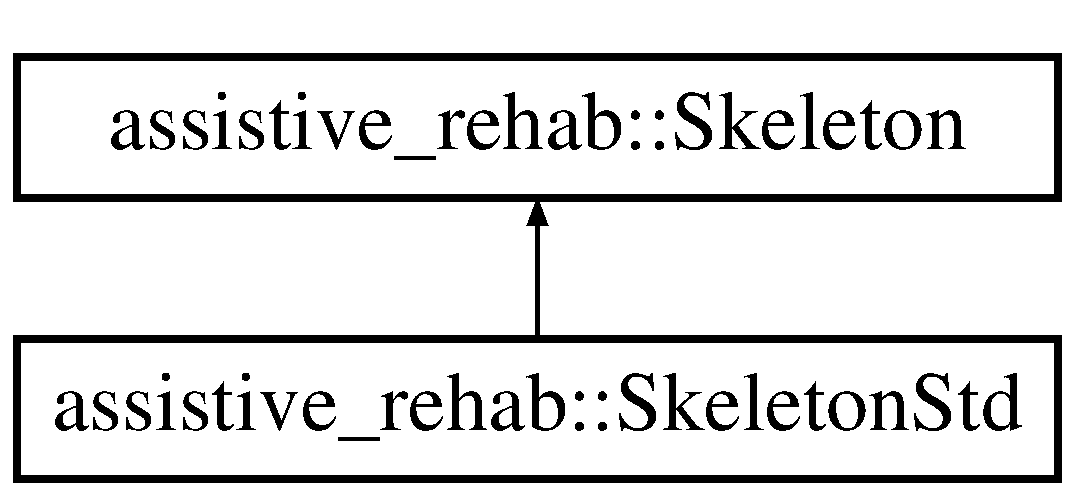
\includegraphics[height=2.000000cm]{classassistive__rehab_1_1Skeleton}
\end{center}
\end{figure}
\subsection*{Public Member Functions}
\begin{DoxyCompactItemize}
\item 
\mbox{\label{classassistive__rehab_1_1Skeleton_af01a02f1ce9ae4c801cd6e66ccf7407f}} 
\hyperlink{classassistive__rehab_1_1Skeleton_af01a02f1ce9ae4c801cd6e66ccf7407f}{Skeleton} ()
\begin{DoxyCompactList}\small\item\em Default constructor. \end{DoxyCompactList}\item 
\mbox{\label{classassistive__rehab_1_1Skeleton_a5bd61b69a0526271e7aa5de41e62200d}} 
\hyperlink{classassistive__rehab_1_1Skeleton_a5bd61b69a0526271e7aa5de41e62200d}{Skeleton} (const \hyperlink{classassistive__rehab_1_1Skeleton}{Skeleton} \&)=delete
\begin{DoxyCompactList}\small\item\em Deleted copy constructor. \end{DoxyCompactList}\item 
\mbox{\label{classassistive__rehab_1_1Skeleton_abedc3e06f870efa7e4b445606a0c1cde}} 
\hyperlink{classassistive__rehab_1_1Skeleton}{Skeleton} \& \hyperlink{classassistive__rehab_1_1Skeleton_abedc3e06f870efa7e4b445606a0c1cde}{operator=} (const \hyperlink{classassistive__rehab_1_1Skeleton}{Skeleton} \&)=delete
\begin{DoxyCompactList}\small\item\em Deleted copy operator. \end{DoxyCompactList}\item 
\mbox{\label{classassistive__rehab_1_1Skeleton_aeece886a4e2f039128144f94f25efd10}} 
virtual \hyperlink{classassistive__rehab_1_1Skeleton_aeece886a4e2f039128144f94f25efd10}{$\sim$\+Skeleton} ()
\begin{DoxyCompactList}\small\item\em Virtual destructor. \end{DoxyCompactList}\item 
const std\+::string \& \hyperlink{classassistive__rehab_1_1Skeleton_a4efc4844bd2b185f1080ee52ab69cb04}{get\+Type} () const
\begin{DoxyCompactList}\small\item\em Return a reference to the type of the skeleton. \end{DoxyCompactList}\item 
void \hyperlink{classassistive__rehab_1_1Skeleton_ae1c830e3d9a0ba692e5ae297caa52a82}{set\+Tag} (const std\+::string \&\hyperlink{classassistive__rehab_1_1Skeleton_a3d1ce5280300e012826948dc4383c2cb}{tag})
\begin{DoxyCompactList}\small\item\em Set the tag of the skeleton. \end{DoxyCompactList}\item 
const std\+::string \& \hyperlink{classassistive__rehab_1_1Skeleton_a185654045d5e43b3853cdb8fdd676da6}{get\+Tag} () const
\begin{DoxyCompactList}\small\item\em Return a reference to the tag of the skeleton. \end{DoxyCompactList}\item 
bool \hyperlink{classassistive__rehab_1_1Skeleton_a3486cbd7f59e75c1d9ef26cbc05bb72f}{set\+Transformation} (const yarp\+::sig\+::\+Matrix \&\hyperlink{classassistive__rehab_1_1Skeleton_a358a1c5eb23a562f8558ff8d43583ef7}{T})
\begin{DoxyCompactList}\small\item\em Set a new transformation matrix of the skeleton. \end{DoxyCompactList}\item 
const yarp\+::sig\+::\+Matrix \& \hyperlink{classassistive__rehab_1_1Skeleton_a2bdcc0d686a5a232aa2c07528cf2e647}{get\+Transformation} () const
\begin{DoxyCompactList}\small\item\em Retrieve the transformation matrix of the skeleton. \end{DoxyCompactList}\item 
bool \hyperlink{classassistive__rehab_1_1Skeleton_ab3bd697f48ea69cfdc5ff7574c19041f}{set\+Coronal} (const yarp\+::sig\+::\+Vector \&\hyperlink{classassistive__rehab_1_1Skeleton_ad042a7e60e6d72cc87b06c5fb0bdfae2}{coronal})
\begin{DoxyCompactList}\small\item\em Set a new coronal plane to the skeleton. \end{DoxyCompactList}\item 
bool \hyperlink{classassistive__rehab_1_1Skeleton_af92fdb0e3eb88a0b1dedd5038e2c6eb7}{set\+Sagittal} (const yarp\+::sig\+::\+Vector \&\hyperlink{classassistive__rehab_1_1Skeleton_a72d6ccb619619e77a17258b08496a972}{sagittal})
\begin{DoxyCompactList}\small\item\em Set a new sagittal plane to the skeleton. \end{DoxyCompactList}\item 
bool \hyperlink{classassistive__rehab_1_1Skeleton_a1aeba05a17363afc08c30397d17375df}{set\+Transverse} (const yarp\+::sig\+::\+Vector \&\hyperlink{classassistive__rehab_1_1Skeleton_ab8a9bf9297f520e8de801248e0b8d2dd}{transverse})
\begin{DoxyCompactList}\small\item\em Set a new transverse plane to the skeleton. \end{DoxyCompactList}\item 
yarp\+::sig\+::\+Vector \hyperlink{classassistive__rehab_1_1Skeleton_aa241a0ac93a9ead198f985073c8935eb}{get\+Coronal} () const
\begin{DoxyCompactList}\small\item\em Retrieve the coronal plane of the skeleton. \end{DoxyCompactList}\item 
yarp\+::sig\+::\+Vector \hyperlink{classassistive__rehab_1_1Skeleton_a83133fabc903ddd4e54edf59df977167}{get\+Sagittal} () const
\begin{DoxyCompactList}\small\item\em Retrieve the sagittal plane of the skeleton. \end{DoxyCompactList}\item 
yarp\+::sig\+::\+Vector \hyperlink{classassistive__rehab_1_1Skeleton_a35c3cdea575eb474a2cb8e0186011cff}{get\+Transverse} () const
\begin{DoxyCompactList}\small\item\em Retrieve the transverse plane of the skeleton. \end{DoxyCompactList}\item 
double \hyperlink{classassistive__rehab_1_1Skeleton_acda9030cd2ed3ad92697418a5e2cff7c}{get\+Max\+Path} () const
\begin{DoxyCompactList}\small\item\em Retrieve the skeleton\textquotesingle{}s maximum path. \end{DoxyCompactList}\item 
virtual yarp\+::os\+::\+Property \hyperlink{classassistive__rehab_1_1Skeleton_ad58ea53a165abc3f39a3c46594f0560f}{to\+Property} ()
\begin{DoxyCompactList}\small\item\em Export the skeleton structure as a property. \end{DoxyCompactList}\item 
virtual void \hyperlink{classassistive__rehab_1_1Skeleton_ac844f66503de87859833056dc33a835b}{from\+Property} (const yarp\+::os\+::\+Property \&prop)
\begin{DoxyCompactList}\small\item\em Import the skeleton structure from its properties. \end{DoxyCompactList}\item 
unsigned int \hyperlink{classassistive__rehab_1_1Skeleton_ac5e5b98f2c9178f6e0def5033e27922f}{get\+Num\+Key\+Points} () const
\begin{DoxyCompactList}\small\item\em Retrieve the number of keypoints of the skeleton. \end{DoxyCompactList}\item 
int \hyperlink{classassistive__rehab_1_1Skeleton_a954bfa99e0dad997ca6d93495246d3f1}{get\+Num\+From\+Key} (const std\+::string \&\hyperlink{classassistive__rehab_1_1Skeleton_a3d1ce5280300e012826948dc4383c2cb}{tag}) const
\begin{DoxyCompactList}\small\item\em Retrieve the index of the keypoint from its tag. \end{DoxyCompactList}\item 
const \hyperlink{classassistive__rehab_1_1KeyPoint}{Key\+Point} $\ast$ \hyperlink{classassistive__rehab_1_1Skeleton_a3ecc7418af653c88e40d41bb379b7271}{operator\mbox{[}$\,$\mbox{]}} (const std\+::string \&\hyperlink{classassistive__rehab_1_1Skeleton_a3d1ce5280300e012826948dc4383c2cb}{tag}) const
\begin{DoxyCompactList}\small\item\em Keypoint access. \end{DoxyCompactList}\item 
const \hyperlink{classassistive__rehab_1_1KeyPoint}{Key\+Point} $\ast$ \hyperlink{classassistive__rehab_1_1Skeleton_a0692ab89f16b0914b9ca9e0d4a07e52c}{operator\mbox{[}$\,$\mbox{]}} (const unsigned int i) const
\begin{DoxyCompactList}\small\item\em Keypoint access. \end{DoxyCompactList}\item 
\mbox{\label{classassistive__rehab_1_1Skeleton_a1ba2ba229331f7966ff1bce10c776d99}} 
virtual void \hyperlink{classassistive__rehab_1_1Skeleton_a1ba2ba229331f7966ff1bce10c776d99}{update} ()
\begin{DoxyCompactList}\small\item\em Update skeleton. \end{DoxyCompactList}\item 
virtual void \hyperlink{classassistive__rehab_1_1Skeleton_adbb387558eac21173b7c82cb43acd603}{update} (const std\+::vector$<$ yarp\+::sig\+::\+Vector $>$ \&ordered)
\begin{DoxyCompactList}\small\item\em Update skeleton from ordered list. \end{DoxyCompactList}\item 
virtual void \hyperlink{classassistive__rehab_1_1Skeleton_ab9642d6621d0a2b189c020f4d7695b14}{update} (const std\+::vector$<$ std\+::pair$<$ std\+::string, yarp\+::sig\+::\+Vector $>$$>$ \&unordered)
\begin{DoxyCompactList}\small\item\em Update skeleton from unordered list. \end{DoxyCompactList}\item 
virtual void \hyperlink{classassistive__rehab_1_1Skeleton_a20d9eb5aecd6dccfa7e049bb932a6cef}{update\+\_\+withpixels} (const std\+::vector$<$ std\+::pair$<$ yarp\+::sig\+::\+Vector, yarp\+::sig\+::\+Vector $>$$>$ \&ordered)
\begin{DoxyCompactList}\small\item\em Update skeleton from ordered list. \end{DoxyCompactList}\item 
virtual void \hyperlink{classassistive__rehab_1_1Skeleton_a36e9dfd4910120025e40ccc3d03c0e01}{update\+\_\+withpixels} (const std\+::vector$<$ std\+::pair$<$ std\+::string, std\+::pair$<$ yarp\+::sig\+::\+Vector, yarp\+::sig\+::\+Vector $>$$>$$>$ \&unordered)
\begin{DoxyCompactList}\small\item\em Update skeleton from unordered list. \end{DoxyCompactList}\item 
virtual void \hyperlink{classassistive__rehab_1_1Skeleton_ae3346b2f363e1812fdc88e59d1f7bf7d}{update} (const yarp\+::os\+::\+Property \&prop)
\begin{DoxyCompactList}\small\item\em Update skeleton from properties. \end{DoxyCompactList}\item 
virtual bool \hyperlink{classassistive__rehab_1_1Skeleton_af0ee2be195f804a9562cb184a2be0bad}{update\+\_\+planes} ()=0
\begin{DoxyCompactList}\small\item\em Update skeleton planes. \end{DoxyCompactList}\item 
virtual std\+::vector$<$ yarp\+::sig\+::\+Vector $>$ \hyperlink{classassistive__rehab_1_1Skeleton_a9c56f7f9e243ae2c4c3fef6dbb051dc2}{get\+\_\+ordered} () const
\begin{DoxyCompactList}\small\item\em Retrieve the ordered list of keypoints. \end{DoxyCompactList}\item 
virtual std\+::vector$<$ std\+::pair$<$ std\+::string, yarp\+::sig\+::\+Vector $>$ $>$ \hyperlink{classassistive__rehab_1_1Skeleton_a7b9f01b2b0f5450920335347c5861a2f}{get\+\_\+unordered} () const
\begin{DoxyCompactList}\small\item\em Retrieve the unordered list of keypoints. \end{DoxyCompactList}\item 
virtual std\+::vector$<$ std\+::pair$<$ yarp\+::sig\+::\+Vector, yarp\+::sig\+::\+Vector $>$ $>$ \hyperlink{classassistive__rehab_1_1Skeleton_a270506cde494cb4261c7892edb46ce53}{get\+\_\+ordered\+\_\+withpixels} () const
\begin{DoxyCompactList}\small\item\em Retrieve the ordered list of keypoints. \end{DoxyCompactList}\item 
virtual std\+::vector$<$ std\+::pair$<$ std\+::string, std\+::pair$<$ yarp\+::sig\+::\+Vector, yarp\+::sig\+::\+Vector $>$ $>$ $>$ \hyperlink{classassistive__rehab_1_1Skeleton_a513a3dc56d55a7b10b256378ae63c6c7}{get\+\_\+unordered\+\_\+withpixels} () const
\begin{DoxyCompactList}\small\item\em Retrieve the unordered list of keypoints. \end{DoxyCompactList}\item 
void \hyperlink{classassistive__rehab_1_1Skeleton_a7753cc8d2b43e27eaf7bf9ef640a99cb}{normalize} (const double n=1.\+0)
\begin{DoxyCompactList}\small\item\em Normalize skeleton in order to have unitary/desired distance among keypoints. \end{DoxyCompactList}\item 
void \hyperlink{classassistive__rehab_1_1Skeleton_a21fded128e2240e4dd507030b7386670}{scale} (const double s)
\begin{DoxyCompactList}\small\item\em Rescale skeleton. \end{DoxyCompactList}\item 
\mbox{\label{classassistive__rehab_1_1Skeleton_a58289ea0ba49220afac3e8d7128493b4}} 
void \hyperlink{classassistive__rehab_1_1Skeleton_a58289ea0ba49220afac3e8d7128493b4}{print} (std\+::ostream \&os=std\+::cout) const
\begin{DoxyCompactList}\small\item\em Print skeleton information. \end{DoxyCompactList}\end{DoxyCompactItemize}
\subsection*{Protected Member Functions}
\begin{DoxyCompactItemize}
\item 
\mbox{\label{classassistive__rehab_1_1Skeleton_ae448d21825bfd36eccb328d16fef995a}} 
yarp\+::os\+::\+Property {\bfseries helper\+\_\+toproperty} (\hyperlink{classassistive__rehab_1_1KeyPoint}{Key\+Point} $\ast$k) const
\item 
\mbox{\label{classassistive__rehab_1_1Skeleton_a8e8fcac9b911ce9eaa0a97b81bffb357}} 
void {\bfseries helper\+\_\+fromproperty} (yarp\+::os\+::\+Bottle $\ast$prop, \hyperlink{classassistive__rehab_1_1KeyPoint}{Key\+Point} $\ast$parent)
\item 
\mbox{\label{classassistive__rehab_1_1Skeleton_a8b1fa988e848ef1fc06439be8eaa19a4}} 
void {\bfseries helper\+\_\+updatefromproperty} (yarp\+::os\+::\+Bottle $\ast$prop)
\item 
\mbox{\label{classassistive__rehab_1_1Skeleton_a574ad07752a2a59ea765e10282998bb4}} 
void {\bfseries helper\+\_\+normalize} (\hyperlink{classassistive__rehab_1_1KeyPoint}{Key\+Point} $\ast$k, const std\+::vector$<$ yarp\+::sig\+::\+Vector $>$ \&helperpoints, const double n)
\item 
\mbox{\label{classassistive__rehab_1_1Skeleton_aefdf8624092fcc2b5458b0be108da01a}} 
void {\bfseries helper\+\_\+scale} (\hyperlink{classassistive__rehab_1_1KeyPoint}{Key\+Point} $\ast$k, const std\+::vector$<$ yarp\+::sig\+::\+Vector $>$ \&helperpoints, const double s)
\item 
\mbox{\label{classassistive__rehab_1_1Skeleton_a66ea19f4fbec2b654e394686180abf43}} 
double {\bfseries helper\+\_\+getmaxpath} (\hyperlink{classassistive__rehab_1_1KeyPoint}{Key\+Point} $\ast$k, std\+::vector$<$ bool $>$ \&visited) const
\end{DoxyCompactItemize}
\subsection*{Protected Attributes}
\begin{DoxyCompactItemize}
\item 
\mbox{\label{classassistive__rehab_1_1Skeleton_a679b826030f01f307d938e583f27d23b}} 
std\+::string \hyperlink{classassistive__rehab_1_1Skeleton_a679b826030f01f307d938e583f27d23b}{type}
\begin{DoxyCompactList}\small\item\em skeleton\textquotesingle{}s type (\char`\"{}assistive\+\_\+rehab\+::\+Skeleton\+Std\char`\"{}) \end{DoxyCompactList}\item 
\mbox{\label{classassistive__rehab_1_1Skeleton_a3d1ce5280300e012826948dc4383c2cb}} 
std\+::string \hyperlink{classassistive__rehab_1_1Skeleton_a3d1ce5280300e012826948dc4383c2cb}{tag}
\begin{DoxyCompactList}\small\item\em skeleton\textquotesingle{}s tag \end{DoxyCompactList}\item 
\mbox{\label{classassistive__rehab_1_1Skeleton_a5f61fbdd10430985cd6754e182226787}} 
std\+::vector$<$ \hyperlink{classassistive__rehab_1_1KeyPoint}{Key\+Point} $\ast$ $>$ \hyperlink{classassistive__rehab_1_1Skeleton_a5f61fbdd10430985cd6754e182226787}{keypoints}
\begin{DoxyCompactList}\small\item\em vector of pointer to \hyperlink{classassistive__rehab_1_1KeyPoint}{Key\+Point} \end{DoxyCompactList}\item 
\mbox{\label{classassistive__rehab_1_1Skeleton_ada4d4b327f1f71520e62e42db9d4c656}} 
std\+::unordered\+\_\+map$<$ std\+::string, \hyperlink{classassistive__rehab_1_1KeyPoint}{Key\+Point} $\ast$ $>$ \hyperlink{classassistive__rehab_1_1Skeleton_ada4d4b327f1f71520e62e42db9d4c656}{tag2key}
\begin{DoxyCompactList}\small\item\em map associating a tag to a pointer to a \hyperlink{classassistive__rehab_1_1KeyPoint}{Key\+Point} \end{DoxyCompactList}\item 
\mbox{\label{classassistive__rehab_1_1Skeleton_a4b1c3607cabb58053e4c367015e98e28}} 
std\+::unordered\+\_\+map$<$ \hyperlink{classassistive__rehab_1_1KeyPoint}{Key\+Point} $\ast$, unsigned int $>$ \hyperlink{classassistive__rehab_1_1Skeleton_a4b1c3607cabb58053e4c367015e98e28}{key2id}
\begin{DoxyCompactList}\small\item\em map associating a pointer to a \hyperlink{classassistive__rehab_1_1KeyPoint}{Key\+Point} to an index \end{DoxyCompactList}\item 
\mbox{\label{classassistive__rehab_1_1Skeleton_a358a1c5eb23a562f8558ff8d43583ef7}} 
yarp\+::sig\+::\+Matrix \hyperlink{classassistive__rehab_1_1Skeleton_a358a1c5eb23a562f8558ff8d43583ef7}{T}
\begin{DoxyCompactList}\small\item\em transformation matrix \end{DoxyCompactList}\item 
\mbox{\label{classassistive__rehab_1_1Skeleton_ad042a7e60e6d72cc87b06c5fb0bdfae2}} 
yarp\+::sig\+::\+Vector \hyperlink{classassistive__rehab_1_1Skeleton_ad042a7e60e6d72cc87b06c5fb0bdfae2}{coronal}
\begin{DoxyCompactList}\small\item\em vector containing the normal to the coronal plane \end{DoxyCompactList}\item 
\mbox{\label{classassistive__rehab_1_1Skeleton_a72d6ccb619619e77a17258b08496a972}} 
yarp\+::sig\+::\+Vector \hyperlink{classassistive__rehab_1_1Skeleton_a72d6ccb619619e77a17258b08496a972}{sagittal}
\begin{DoxyCompactList}\small\item\em vector containing the normal to the sagittal plane \end{DoxyCompactList}\item 
\mbox{\label{classassistive__rehab_1_1Skeleton_ab8a9bf9297f520e8de801248e0b8d2dd}} 
yarp\+::sig\+::\+Vector \hyperlink{classassistive__rehab_1_1Skeleton_ab8a9bf9297f520e8de801248e0b8d2dd}{transverse}
\begin{DoxyCompactList}\small\item\em vector containing the normal to the transverse plane \end{DoxyCompactList}\end{DoxyCompactItemize}


\subsection{Detailed Description}
Abstract class for skeleton. 

Definition at line 220 of file skeleton.\+h.



\subsection{Member Function Documentation}
\mbox{\label{classassistive__rehab_1_1Skeleton_ac844f66503de87859833056dc33a835b}} 
\index{assistive\+\_\+rehab\+::\+Skeleton@{assistive\+\_\+rehab\+::\+Skeleton}!from\+Property@{from\+Property}}
\index{from\+Property@{from\+Property}!assistive\+\_\+rehab\+::\+Skeleton@{assistive\+\_\+rehab\+::\+Skeleton}}
\subsubsection{\texorpdfstring{from\+Property()}{fromProperty()}}
{\footnotesize\ttfamily void Skeleton\+::from\+Property (\begin{DoxyParamCaption}\item[{const yarp\+::os\+::\+Property \&}]{prop }\end{DoxyParamCaption})\hspace{0.3cm}{\ttfamily [virtual]}}



Import the skeleton structure from its properties. 


\begin{DoxyParams}{Parameters}
{\em prop} & Property object containing the properties of a skeleton.\\
\hline
\end{DoxyParams}
Available properties are\+:
\begin{DoxyItemize}
\item type\+: string containing skeleton\textquotesingle{}s type (\char`\"{}assistive\+\_\+rehab\+::\+Skeleton\+Std\char`\"{}).
\item tag\+: string containing skeleton\textquotesingle{}s tag.
\item transformation\+: 4 x 4 skeleton\textquotesingle{}s roto-\/translation matrix.
\item coronal\+: vector containing skeleton\textquotesingle{}s coronal plane.
\item sagittal\+: vector containing skeleton\textquotesingle{}s sagittal plane.
\item transverse\+: vector containing skeleton\textquotesingle{}s transverse plane.
\item skeleton\+: list containing keypoints with the following subproperties\+:
\begin{DoxyItemize}
\item tag\+: string containing keypoint\textquotesingle{}s tag.
\item status\+: string containing keypoint\textquotesingle{}s status (updated or stale).
\item position\+: vector containing keypoint\textquotesingle{}s camera coordinates x,y,z.
\item pixel\+: vector containing keypoint\textquotesingle{}s image coordinates u,v.
\item child\+: list containing keypoint\textquotesingle{}s child, specified as position, status, tag. 
\end{DoxyItemize}
\end{DoxyItemize}

Definition at line 400 of file skeleton.\+cpp.



Referenced by assistive\+\_\+rehab\+::\+Skeleton\+Std\+::update\+\_\+planes().


\begin{DoxyCode}
401 \{
402     \textcolor{keywordflow}{for} (\textcolor{keyword}{auto} &k:keypoints)
403         \textcolor{keyword}{delete} k;
404 
405     keypoints.clear();
406     tag2key.clear();
407     key2id.clear();
408 
409     tag=prop.check(\textcolor{stringliteral}{"tag"},Value(\textcolor{stringliteral}{""})).asString();
410     \textcolor{keywordflow}{if} (prop.check(\textcolor{stringliteral}{"transformation"}))
411     \{
412         \textcolor{keywordflow}{if} (Bottle *b=prop.find(\textcolor{stringliteral}{"transformation"}).asList())
413             b->write(T);
414     \}
415     \textcolor{keywordflow}{else}
416         T=eye(4,4);
417 
418     coronal=sagittal=transverse=zeros(3);
419     \textcolor{keywordflow}{if} (prop.check(\textcolor{stringliteral}{"coronal"}))
420         \textcolor{keywordflow}{if} (Bottle *b=prop.find(\textcolor{stringliteral}{"coronal"}).asList())
421             b->write(coronal);
422     \textcolor{keywordflow}{if} (prop.check(\textcolor{stringliteral}{"sagittal"}))
423         \textcolor{keywordflow}{if} (Bottle *b=prop.find(\textcolor{stringliteral}{"sagittal"}).asList())
424             b->write(sagittal);
425     \textcolor{keywordflow}{if} (prop.check(\textcolor{stringliteral}{"transverse"}))
426         \textcolor{keywordflow}{if} (Bottle *b=prop.find(\textcolor{stringliteral}{"transverse"}).asList())
427             b->write(transverse);
428     helper\_fromproperty(prop.find(\textcolor{stringliteral}{"skeleton"}).asList(),\textcolor{keyword}{nullptr});
429 \}
\end{DoxyCode}
\mbox{\label{classassistive__rehab_1_1Skeleton_a9c56f7f9e243ae2c4c3fef6dbb051dc2}} 
\index{assistive\+\_\+rehab\+::\+Skeleton@{assistive\+\_\+rehab\+::\+Skeleton}!get\+\_\+ordered@{get\+\_\+ordered}}
\index{get\+\_\+ordered@{get\+\_\+ordered}!assistive\+\_\+rehab\+::\+Skeleton@{assistive\+\_\+rehab\+::\+Skeleton}}
\subsubsection{\texorpdfstring{get\+\_\+ordered()}{get\_ordered()}}
{\footnotesize\ttfamily vector$<$ Vector $>$ Skeleton\+::get\+\_\+ordered (\begin{DoxyParamCaption}{ }\end{DoxyParamCaption}) const\hspace{0.3cm}{\ttfamily [virtual]}}



Retrieve the ordered list of keypoints. 

\begin{DoxyReturn}{Returns}
vector containing the ordered list of keypoints, each specified as vector containing the x,y,z camera coordinates. 
\end{DoxyReturn}


Definition at line 581 of file skeleton.\+cpp.



References assistive\+\_\+rehab\+::\+Key\+Point\+::get\+Point().


\begin{DoxyCode}
582 \{
583     vector<Vector> ordered;
584     \textcolor{keywordflow}{for} (\textcolor{keyword}{auto} &k:keypoints)
585         ordered.push\_back(k->getPoint());
586     \textcolor{keywordflow}{return} ordered;
587 \}
\end{DoxyCode}
\mbox{\label{classassistive__rehab_1_1Skeleton_a270506cde494cb4261c7892edb46ce53}} 
\index{assistive\+\_\+rehab\+::\+Skeleton@{assistive\+\_\+rehab\+::\+Skeleton}!get\+\_\+ordered\+\_\+withpixels@{get\+\_\+ordered\+\_\+withpixels}}
\index{get\+\_\+ordered\+\_\+withpixels@{get\+\_\+ordered\+\_\+withpixels}!assistive\+\_\+rehab\+::\+Skeleton@{assistive\+\_\+rehab\+::\+Skeleton}}
\subsubsection{\texorpdfstring{get\+\_\+ordered\+\_\+withpixels()}{get\_ordered\_withpixels()}}
{\footnotesize\ttfamily vector$<$ pair$<$ Vector, Vector $>$ $>$ Skeleton\+::get\+\_\+ordered\+\_\+withpixels (\begin{DoxyParamCaption}{ }\end{DoxyParamCaption}) const\hspace{0.3cm}{\ttfamily [virtual]}}



Retrieve the ordered list of keypoints. 

\begin{DoxyReturn}{Returns}
vector containing the ordered list of keypoints, each specified as a pair of vectors with x,y,z and u,v coordinates. 
\end{DoxyReturn}


Definition at line 597 of file skeleton.\+cpp.



References assistive\+\_\+rehab\+::\+Key\+Point\+::get\+Pixel(), and assistive\+\_\+rehab\+::\+Key\+Point\+::get\+Point().


\begin{DoxyCode}
598 \{
599     vector<pair<Vector,Vector>> ordered;
600     \textcolor{keywordflow}{for} (\textcolor{keyword}{auto} &k:keypoints)
601         ordered.push\_back(make\_pair(k->getPoint(),k->getPixel()));
602     \textcolor{keywordflow}{return} ordered;
603 \}
\end{DoxyCode}
\mbox{\label{classassistive__rehab_1_1Skeleton_a7b9f01b2b0f5450920335347c5861a2f}} 
\index{assistive\+\_\+rehab\+::\+Skeleton@{assistive\+\_\+rehab\+::\+Skeleton}!get\+\_\+unordered@{get\+\_\+unordered}}
\index{get\+\_\+unordered@{get\+\_\+unordered}!assistive\+\_\+rehab\+::\+Skeleton@{assistive\+\_\+rehab\+::\+Skeleton}}
\subsubsection{\texorpdfstring{get\+\_\+unordered()}{get\_unordered()}}
{\footnotesize\ttfamily vector$<$ pair$<$ string, Vector $>$ $>$ Skeleton\+::get\+\_\+unordered (\begin{DoxyParamCaption}{ }\end{DoxyParamCaption}) const\hspace{0.3cm}{\ttfamily [virtual]}}



Retrieve the unordered list of keypoints. 

\begin{DoxyReturn}{Returns}
vector containing an unordered list of keypoints, each specified as pair which associates a string, containing the keypoint\textquotesingle{}s tag, and a vector, containing the x,y,z camera coordinates. 
\end{DoxyReturn}


Definition at line 589 of file skeleton.\+cpp.


\begin{DoxyCode}
590 \{
591     vector<pair<string,Vector>> unordered;
592     \textcolor{keywordflow}{for} (\textcolor{keyword}{auto} &it:tag2key)
593         unordered.push\_back(make\_pair(it.first,it.second->getPoint()));
594     \textcolor{keywordflow}{return} unordered;
595 \}
\end{DoxyCode}
\mbox{\label{classassistive__rehab_1_1Skeleton_a513a3dc56d55a7b10b256378ae63c6c7}} 
\index{assistive\+\_\+rehab\+::\+Skeleton@{assistive\+\_\+rehab\+::\+Skeleton}!get\+\_\+unordered\+\_\+withpixels@{get\+\_\+unordered\+\_\+withpixels}}
\index{get\+\_\+unordered\+\_\+withpixels@{get\+\_\+unordered\+\_\+withpixels}!assistive\+\_\+rehab\+::\+Skeleton@{assistive\+\_\+rehab\+::\+Skeleton}}
\subsubsection{\texorpdfstring{get\+\_\+unordered\+\_\+withpixels()}{get\_unordered\_withpixels()}}
{\footnotesize\ttfamily vector$<$ pair$<$ string, pair$<$ Vector, Vector $>$ $>$ $>$ Skeleton\+::get\+\_\+unordered\+\_\+withpixels (\begin{DoxyParamCaption}{ }\end{DoxyParamCaption}) const\hspace{0.3cm}{\ttfamily [virtual]}}



Retrieve the unordered list of keypoints. 

\begin{DoxyReturn}{Returns}
vector containing an unordered list of keypoints, each specified as pair that associates a string containing the keypoint\textquotesingle{}s tag to a pair of vectors of x,y,z and u,v coordinates. 
\end{DoxyReturn}


Definition at line 605 of file skeleton.\+cpp.


\begin{DoxyCode}
606 \{
607     vector<pair<string,pair<Vector,Vector>>> unordered;
608     \textcolor{keywordflow}{for} (\textcolor{keyword}{auto} &it:tag2key)
609         unordered.push\_back(make\_pair(it.first,make\_pair(it.second->getPoint(),it.second->getPixel())));
610     \textcolor{keywordflow}{return} unordered;
611 \}
\end{DoxyCode}
\mbox{\label{classassistive__rehab_1_1Skeleton_aa241a0ac93a9ead198f985073c8935eb}} 
\index{assistive\+\_\+rehab\+::\+Skeleton@{assistive\+\_\+rehab\+::\+Skeleton}!get\+Coronal@{get\+Coronal}}
\index{get\+Coronal@{get\+Coronal}!assistive\+\_\+rehab\+::\+Skeleton@{assistive\+\_\+rehab\+::\+Skeleton}}
\subsubsection{\texorpdfstring{get\+Coronal()}{getCoronal()}}
{\footnotesize\ttfamily Vector Skeleton\+::get\+Coronal (\begin{DoxyParamCaption}{ }\end{DoxyParamCaption}) const}



Retrieve the coronal plane of the skeleton. 

\begin{DoxyReturn}{Returns}
vector containing x,y,z coordinates of the normal to skeleton\textquotesingle{}s coronal plane. 
\end{DoxyReturn}


Definition at line 340 of file skeleton.\+cpp.


\begin{DoxyCode}
341 \{
342     \textcolor{keywordflow}{return} (T.submatrix(0,2,0,2)*coronal);
343 \}
\end{DoxyCode}
\mbox{\label{classassistive__rehab_1_1Skeleton_acda9030cd2ed3ad92697418a5e2cff7c}} 
\index{assistive\+\_\+rehab\+::\+Skeleton@{assistive\+\_\+rehab\+::\+Skeleton}!get\+Max\+Path@{get\+Max\+Path}}
\index{get\+Max\+Path@{get\+Max\+Path}!assistive\+\_\+rehab\+::\+Skeleton@{assistive\+\_\+rehab\+::\+Skeleton}}
\subsubsection{\texorpdfstring{get\+Max\+Path()}{getMaxPath()}}
{\footnotesize\ttfamily double Skeleton\+::get\+Max\+Path (\begin{DoxyParamCaption}{ }\end{DoxyParamCaption}) const}



Retrieve the skeleton\textquotesingle{}s maximum path. 

\begin{DoxyReturn}{Returns}
skeleton\textquotesingle{}s maximum path. 
\end{DoxyReturn}


Definition at line 355 of file skeleton.\+cpp.


\begin{DoxyCode}
356 \{
357     Vector paths(1,0.0);
358     \textcolor{keywordflow}{for} (\textcolor{keyword}{auto} &k:keypoints)
359     \{
360         vector<bool> visited(getNumKeyPoints(),\textcolor{keyword}{false});
361         paths.push\_back(helper\_getmaxpath(k,visited));
362     \}
363     \textcolor{keywordflow}{return} findMax(paths);
364 \}
\end{DoxyCode}
\mbox{\label{classassistive__rehab_1_1Skeleton_a954bfa99e0dad997ca6d93495246d3f1}} 
\index{assistive\+\_\+rehab\+::\+Skeleton@{assistive\+\_\+rehab\+::\+Skeleton}!get\+Num\+From\+Key@{get\+Num\+From\+Key}}
\index{get\+Num\+From\+Key@{get\+Num\+From\+Key}!assistive\+\_\+rehab\+::\+Skeleton@{assistive\+\_\+rehab\+::\+Skeleton}}
\subsubsection{\texorpdfstring{get\+Num\+From\+Key()}{getNumFromKey()}}
{\footnotesize\ttfamily int Skeleton\+::get\+Num\+From\+Key (\begin{DoxyParamCaption}\item[{const std\+::string \&}]{tag }\end{DoxyParamCaption}) const}



Retrieve the index of the keypoint from its tag. 


\begin{DoxyParams}{Parameters}
{\em tag} & string containing the keypoint\textquotesingle{}s tag. \\
\hline
\end{DoxyParams}
\begin{DoxyReturn}{Returns}
skeleton\textquotesingle{}s number of keypoints. 
\end{DoxyReturn}


Definition at line 431 of file skeleton.\+cpp.



References operator\mbox{[}$\,$\mbox{]}().


\begin{DoxyCode}
432 \{
433     \textcolor{keyword}{auto} it1=tag2key.find(tag);
434     \textcolor{keywordflow}{if} (it1!=tag2key.end())
435     \{
436         \textcolor{keyword}{auto} it2=key2id.find(it1->second);
437         \textcolor{keywordflow}{if} (it2!=key2id.end())
438             \textcolor{keywordflow}{return} (\textcolor{keywordtype}{int})it2->second;
439     \}
440     \textcolor{keywordflow}{return} -1;
441 \}
\end{DoxyCode}
\mbox{\label{classassistive__rehab_1_1Skeleton_ac5e5b98f2c9178f6e0def5033e27922f}} 
\index{assistive\+\_\+rehab\+::\+Skeleton@{assistive\+\_\+rehab\+::\+Skeleton}!get\+Num\+Key\+Points@{get\+Num\+Key\+Points}}
\index{get\+Num\+Key\+Points@{get\+Num\+Key\+Points}!assistive\+\_\+rehab\+::\+Skeleton@{assistive\+\_\+rehab\+::\+Skeleton}}
\subsubsection{\texorpdfstring{get\+Num\+Key\+Points()}{getNumKeyPoints()}}
{\footnotesize\ttfamily unsigned int assistive\+\_\+rehab\+::\+Skeleton\+::get\+Num\+Key\+Points (\begin{DoxyParamCaption}{ }\end{DoxyParamCaption}) const\hspace{0.3cm}{\ttfamily [inline]}}



Retrieve the number of keypoints of the skeleton. 

\begin{DoxyReturn}{Returns}
skeleton\textquotesingle{}s number of keypoints. 
\end{DoxyReturn}


Definition at line 383 of file skeleton.\+h.


\begin{DoxyCode}
383 \{ \textcolor{keywordflow}{return} (\textcolor{keywordtype}{unsigned} \textcolor{keywordtype}{int})keypoints.size(); \}
\end{DoxyCode}
\mbox{\label{classassistive__rehab_1_1Skeleton_a83133fabc903ddd4e54edf59df977167}} 
\index{assistive\+\_\+rehab\+::\+Skeleton@{assistive\+\_\+rehab\+::\+Skeleton}!get\+Sagittal@{get\+Sagittal}}
\index{get\+Sagittal@{get\+Sagittal}!assistive\+\_\+rehab\+::\+Skeleton@{assistive\+\_\+rehab\+::\+Skeleton}}
\subsubsection{\texorpdfstring{get\+Sagittal()}{getSagittal()}}
{\footnotesize\ttfamily Vector Skeleton\+::get\+Sagittal (\begin{DoxyParamCaption}{ }\end{DoxyParamCaption}) const}



Retrieve the sagittal plane of the skeleton. 

\begin{DoxyReturn}{Returns}
vector containing the x,y,z coordinates of the normal skeleton\textquotesingle{}s sagittal plane. 
\end{DoxyReturn}


Definition at line 345 of file skeleton.\+cpp.


\begin{DoxyCode}
346 \{
347     \textcolor{keywordflow}{return} (T.submatrix(0,2,0,2)*sagittal);
348 \}
\end{DoxyCode}
\mbox{\label{classassistive__rehab_1_1Skeleton_a185654045d5e43b3853cdb8fdd676da6}} 
\index{assistive\+\_\+rehab\+::\+Skeleton@{assistive\+\_\+rehab\+::\+Skeleton}!get\+Tag@{get\+Tag}}
\index{get\+Tag@{get\+Tag}!assistive\+\_\+rehab\+::\+Skeleton@{assistive\+\_\+rehab\+::\+Skeleton}}
\subsubsection{\texorpdfstring{get\+Tag()}{getTag()}}
{\footnotesize\ttfamily const std\+::string\& assistive\+\_\+rehab\+::\+Skeleton\+::get\+Tag (\begin{DoxyParamCaption}{ }\end{DoxyParamCaption}) const\hspace{0.3cm}{\ttfamily [inline]}}



Return a reference to the tag of the skeleton. 

\begin{DoxyReturn}{Returns}
reference to a string containing the skeleton\textquotesingle{}s tag. 
\end{DoxyReturn}


Definition at line 278 of file skeleton.\+h.


\begin{DoxyCode}
278 \{ \textcolor{keywordflow}{return} tag; \}
\end{DoxyCode}
\mbox{\label{classassistive__rehab_1_1Skeleton_a2bdcc0d686a5a232aa2c07528cf2e647}} 
\index{assistive\+\_\+rehab\+::\+Skeleton@{assistive\+\_\+rehab\+::\+Skeleton}!get\+Transformation@{get\+Transformation}}
\index{get\+Transformation@{get\+Transformation}!assistive\+\_\+rehab\+::\+Skeleton@{assistive\+\_\+rehab\+::\+Skeleton}}
\subsubsection{\texorpdfstring{get\+Transformation()}{getTransformation()}}
{\footnotesize\ttfamily const yarp\+::sig\+::\+Matrix\& assistive\+\_\+rehab\+::\+Skeleton\+::get\+Transformation (\begin{DoxyParamCaption}{ }\end{DoxyParamCaption}) const\hspace{0.3cm}{\ttfamily [inline]}}



Retrieve the transformation matrix of the skeleton. 

\begin{DoxyReturn}{Returns}
reference to the skeleton\textquotesingle{}s transformation matrix. 
\end{DoxyReturn}
\begin{DoxyNote}{Note}
if the transformation matrix is the identity matrix, keypoints are defined with respect to the camera. 
\end{DoxyNote}


Definition at line 291 of file skeleton.\+h.


\begin{DoxyCode}
291 \{ \textcolor{keywordflow}{return} T; \}
\end{DoxyCode}
\mbox{\label{classassistive__rehab_1_1Skeleton_a35c3cdea575eb474a2cb8e0186011cff}} 
\index{assistive\+\_\+rehab\+::\+Skeleton@{assistive\+\_\+rehab\+::\+Skeleton}!get\+Transverse@{get\+Transverse}}
\index{get\+Transverse@{get\+Transverse}!assistive\+\_\+rehab\+::\+Skeleton@{assistive\+\_\+rehab\+::\+Skeleton}}
\subsubsection{\texorpdfstring{get\+Transverse()}{getTransverse()}}
{\footnotesize\ttfamily Vector Skeleton\+::get\+Transverse (\begin{DoxyParamCaption}{ }\end{DoxyParamCaption}) const}



Retrieve the transverse plane of the skeleton. 

\begin{DoxyReturn}{Returns}
vector containing the x,y,z coordinates of the normal skeleton\textquotesingle{}s sagittal plane. 
\end{DoxyReturn}


Definition at line 350 of file skeleton.\+cpp.


\begin{DoxyCode}
351 \{
352     \textcolor{keywordflow}{return} (T.submatrix(0,2,0,2)*transverse);
353 \}
\end{DoxyCode}
\mbox{\label{classassistive__rehab_1_1Skeleton_a4efc4844bd2b185f1080ee52ab69cb04}} 
\index{assistive\+\_\+rehab\+::\+Skeleton@{assistive\+\_\+rehab\+::\+Skeleton}!get\+Type@{get\+Type}}
\index{get\+Type@{get\+Type}!assistive\+\_\+rehab\+::\+Skeleton@{assistive\+\_\+rehab\+::\+Skeleton}}
\subsubsection{\texorpdfstring{get\+Type()}{getType()}}
{\footnotesize\ttfamily const std\+::string\& assistive\+\_\+rehab\+::\+Skeleton\+::get\+Type (\begin{DoxyParamCaption}{ }\end{DoxyParamCaption}) const\hspace{0.3cm}{\ttfamily [inline]}}



Return a reference to the type of the skeleton. 

\begin{DoxyReturn}{Returns}
reference to the skeleton\textquotesingle{}s type. 
\end{DoxyReturn}


Definition at line 266 of file skeleton.\+h.


\begin{DoxyCode}
266 \{ \textcolor{keywordflow}{return} type; \}
\end{DoxyCode}
\mbox{\label{classassistive__rehab_1_1Skeleton_a7753cc8d2b43e27eaf7bf9ef640a99cb}} 
\index{assistive\+\_\+rehab\+::\+Skeleton@{assistive\+\_\+rehab\+::\+Skeleton}!normalize@{normalize}}
\index{normalize@{normalize}!assistive\+\_\+rehab\+::\+Skeleton@{assistive\+\_\+rehab\+::\+Skeleton}}
\subsubsection{\texorpdfstring{normalize()}{normalize()}}
{\footnotesize\ttfamily void Skeleton\+::normalize (\begin{DoxyParamCaption}\item[{const double}]{n = {\ttfamily 1.0} }\end{DoxyParamCaption})}



Normalize skeleton in order to have unitary/desired distance among keypoints. 


\begin{DoxyParams}{Parameters}
{\em n} & double containing the normalization factor. \\
\hline
\end{DoxyParams}


Definition at line 613 of file skeleton.\+cpp.



References assistive\+\_\+rehab\+::\+Key\+Point\+::get\+Point().


\begin{DoxyCode}
614 \{
615     \textcolor{keywordflow}{if} (keypoints.size()>0)
616     \{
617         vector<Vector> helperpoints;
618         \textcolor{keywordflow}{for} (\textcolor{keyword}{auto} &k:keypoints)
619             helperpoints.push\_back(k->getPoint());
620         helper\_normalize(keypoints[0],helperpoints,n);
621     \}
622 \}
\end{DoxyCode}
\mbox{\label{classassistive__rehab_1_1Skeleton_a3ecc7418af653c88e40d41bb379b7271}} 
\index{assistive\+\_\+rehab\+::\+Skeleton@{assistive\+\_\+rehab\+::\+Skeleton}!operator\mbox{[}\mbox{]}@{operator[]}}
\index{operator\mbox{[}\mbox{]}@{operator[]}!assistive\+\_\+rehab\+::\+Skeleton@{assistive\+\_\+rehab\+::\+Skeleton}}
\subsubsection{\texorpdfstring{operator[]()}{operator[]()}\hspace{0.1cm}{\footnotesize\ttfamily [1/2]}}
{\footnotesize\ttfamily const \hyperlink{classassistive__rehab_1_1KeyPoint}{Key\+Point}$\ast$ assistive\+\_\+rehab\+::\+Skeleton\+::operator\mbox{[}$\,$\mbox{]} (\begin{DoxyParamCaption}\item[{const std\+::string \&}]{tag }\end{DoxyParamCaption}) const}



Keypoint access. 

Returns a pointer to the keypoint specified by its tag. 
\begin{DoxyParams}{Parameters}
{\em tag} & string containing the keypoint\textquotesingle{}s tag. \\
\hline
\end{DoxyParams}
\begin{DoxyReturn}{Returns}
a (const) pointer to the keypoint. 
\end{DoxyReturn}


Referenced by get\+Num\+From\+Key().

\mbox{\label{classassistive__rehab_1_1Skeleton_a0692ab89f16b0914b9ca9e0d4a07e52c}} 
\index{assistive\+\_\+rehab\+::\+Skeleton@{assistive\+\_\+rehab\+::\+Skeleton}!operator\mbox{[}\mbox{]}@{operator[]}}
\index{operator\mbox{[}\mbox{]}@{operator[]}!assistive\+\_\+rehab\+::\+Skeleton@{assistive\+\_\+rehab\+::\+Skeleton}}
\subsubsection{\texorpdfstring{operator[]()}{operator[]()}\hspace{0.1cm}{\footnotesize\ttfamily [2/2]}}
{\footnotesize\ttfamily const \hyperlink{classassistive__rehab_1_1KeyPoint}{Key\+Point} $\ast$ Skeleton\+::operator\mbox{[}$\,$\mbox{]} (\begin{DoxyParamCaption}\item[{const unsigned int}]{i }\end{DoxyParamCaption}) const}



Keypoint access. 

Returns a pointer to the keypoint specified by its index. 
\begin{DoxyParams}{Parameters}
{\em i} & int containing the keypoint\textquotesingle{}s index. \\
\hline
\end{DoxyParams}
\begin{DoxyReturn}{Returns}
a (const) pointer to the keypoint. 
\end{DoxyReturn}


Definition at line 449 of file skeleton.\+cpp.


\begin{DoxyCode}
450 \{
451     \textcolor{keywordflow}{return} (i<keypoints.size())?keypoints[i]:\textcolor{keyword}{nullptr};
452 \}
\end{DoxyCode}
\mbox{\label{classassistive__rehab_1_1Skeleton_a21fded128e2240e4dd507030b7386670}} 
\index{assistive\+\_\+rehab\+::\+Skeleton@{assistive\+\_\+rehab\+::\+Skeleton}!scale@{scale}}
\index{scale@{scale}!assistive\+\_\+rehab\+::\+Skeleton@{assistive\+\_\+rehab\+::\+Skeleton}}
\subsubsection{\texorpdfstring{scale()}{scale()}}
{\footnotesize\ttfamily void Skeleton\+::scale (\begin{DoxyParamCaption}\item[{const double}]{s }\end{DoxyParamCaption})}



Rescale skeleton. 


\begin{DoxyParams}{Parameters}
{\em s} & double containing the scaling factor. \\
\hline
\end{DoxyParams}


Definition at line 624 of file skeleton.\+cpp.



References assistive\+\_\+rehab\+::\+Key\+Point\+::get\+Point().


\begin{DoxyCode}
625 \{
626     \textcolor{keywordflow}{if} (keypoints.size()>0)
627     \{
628         vector<Vector> helperpoints;
629         \textcolor{keywordflow}{for} (\textcolor{keyword}{auto} &k:keypoints)
630             helperpoints.push\_back(k->getPoint());
631         helper\_scale(keypoints[0],helperpoints,s);
632     \}
633 \}
\end{DoxyCode}
\mbox{\label{classassistive__rehab_1_1Skeleton_ab3bd697f48ea69cfdc5ff7574c19041f}} 
\index{assistive\+\_\+rehab\+::\+Skeleton@{assistive\+\_\+rehab\+::\+Skeleton}!set\+Coronal@{set\+Coronal}}
\index{set\+Coronal@{set\+Coronal}!assistive\+\_\+rehab\+::\+Skeleton@{assistive\+\_\+rehab\+::\+Skeleton}}
\subsubsection{\texorpdfstring{set\+Coronal()}{setCoronal()}}
{\footnotesize\ttfamily bool Skeleton\+::set\+Coronal (\begin{DoxyParamCaption}\item[{const yarp\+::sig\+::\+Vector \&}]{coronal }\end{DoxyParamCaption})}



Set a new coronal plane to the skeleton. 


\begin{DoxyParams}{Parameters}
{\em coronal} & vector containing the x,y,z coordinates of the normal to the desired plane. \\
\hline
\end{DoxyParams}


Definition at line 307 of file skeleton.\+cpp.


\begin{DoxyCode}
308 \{
309     \textcolor{keywordflow}{if} (coronal.length()>=3)
310     \{
311         this->coronal=coronal.subVector(0,2);
312         \textcolor{keywordflow}{return} \textcolor{keyword}{true};
313     \}
314     \textcolor{keywordflow}{else}
315         \textcolor{keywordflow}{return} \textcolor{keyword}{false};
316 \}
\end{DoxyCode}
\mbox{\label{classassistive__rehab_1_1Skeleton_af92fdb0e3eb88a0b1dedd5038e2c6eb7}} 
\index{assistive\+\_\+rehab\+::\+Skeleton@{assistive\+\_\+rehab\+::\+Skeleton}!set\+Sagittal@{set\+Sagittal}}
\index{set\+Sagittal@{set\+Sagittal}!assistive\+\_\+rehab\+::\+Skeleton@{assistive\+\_\+rehab\+::\+Skeleton}}
\subsubsection{\texorpdfstring{set\+Sagittal()}{setSagittal()}}
{\footnotesize\ttfamily bool Skeleton\+::set\+Sagittal (\begin{DoxyParamCaption}\item[{const yarp\+::sig\+::\+Vector \&}]{sagittal }\end{DoxyParamCaption})}



Set a new sagittal plane to the skeleton. 


\begin{DoxyParams}{Parameters}
{\em sagittal} & vector containing the x,y,z coordinates of the normal to the desired plane. \\
\hline
\end{DoxyParams}


Definition at line 318 of file skeleton.\+cpp.


\begin{DoxyCode}
319 \{
320     \textcolor{keywordflow}{if} (sagittal.length()>=3)
321     \{
322         this->sagittal=sagittal.subVector(0,2);
323         \textcolor{keywordflow}{return} \textcolor{keyword}{true};
324     \}
325     \textcolor{keywordflow}{else}
326         \textcolor{keywordflow}{return} \textcolor{keyword}{false};
327 \}
\end{DoxyCode}
\mbox{\label{classassistive__rehab_1_1Skeleton_ae1c830e3d9a0ba692e5ae297caa52a82}} 
\index{assistive\+\_\+rehab\+::\+Skeleton@{assistive\+\_\+rehab\+::\+Skeleton}!set\+Tag@{set\+Tag}}
\index{set\+Tag@{set\+Tag}!assistive\+\_\+rehab\+::\+Skeleton@{assistive\+\_\+rehab\+::\+Skeleton}}
\subsubsection{\texorpdfstring{set\+Tag()}{setTag()}}
{\footnotesize\ttfamily void assistive\+\_\+rehab\+::\+Skeleton\+::set\+Tag (\begin{DoxyParamCaption}\item[{const std\+::string \&}]{tag }\end{DoxyParamCaption})\hspace{0.3cm}{\ttfamily [inline]}}



Set the tag of the skeleton. 


\begin{DoxyParams}{Parameters}
{\em tag} & string containing the desired tag. \\
\hline
\end{DoxyParams}


Definition at line 272 of file skeleton.\+h.


\begin{DoxyCode}
272 \{ this->tag=tag; \}
\end{DoxyCode}
\mbox{\label{classassistive__rehab_1_1Skeleton_a3486cbd7f59e75c1d9ef26cbc05bb72f}} 
\index{assistive\+\_\+rehab\+::\+Skeleton@{assistive\+\_\+rehab\+::\+Skeleton}!set\+Transformation@{set\+Transformation}}
\index{set\+Transformation@{set\+Transformation}!assistive\+\_\+rehab\+::\+Skeleton@{assistive\+\_\+rehab\+::\+Skeleton}}
\subsubsection{\texorpdfstring{set\+Transformation()}{setTransformation()}}
{\footnotesize\ttfamily bool Skeleton\+::set\+Transformation (\begin{DoxyParamCaption}\item[{const yarp\+::sig\+::\+Matrix \&}]{T }\end{DoxyParamCaption})}



Set a new transformation matrix of the skeleton. 


\begin{DoxyParams}{Parameters}
{\em T} & matrix containing the desired transformation. \\
\hline
\end{DoxyParams}


Definition at line 296 of file skeleton.\+cpp.


\begin{DoxyCode}
297 \{
298     \textcolor{keywordflow}{if} ((T.rows()>=4) || (T.cols()>=4))
299     \{
300         this->T=T.submatrix(0,3,0,3);
301         \textcolor{keywordflow}{return} \textcolor{keyword}{true};
302     \}
303     \textcolor{keywordflow}{else}
304         \textcolor{keywordflow}{return} \textcolor{keyword}{false};
305 \}
\end{DoxyCode}
\mbox{\label{classassistive__rehab_1_1Skeleton_a1aeba05a17363afc08c30397d17375df}} 
\index{assistive\+\_\+rehab\+::\+Skeleton@{assistive\+\_\+rehab\+::\+Skeleton}!set\+Transverse@{set\+Transverse}}
\index{set\+Transverse@{set\+Transverse}!assistive\+\_\+rehab\+::\+Skeleton@{assistive\+\_\+rehab\+::\+Skeleton}}
\subsubsection{\texorpdfstring{set\+Transverse()}{setTransverse()}}
{\footnotesize\ttfamily bool Skeleton\+::set\+Transverse (\begin{DoxyParamCaption}\item[{const yarp\+::sig\+::\+Vector \&}]{transverse }\end{DoxyParamCaption})}



Set a new transverse plane to the skeleton. 


\begin{DoxyParams}{Parameters}
{\em transverse} & vector containing the x,y,z coordinates of the normal to the desired plane. \\
\hline
\end{DoxyParams}


Definition at line 329 of file skeleton.\+cpp.


\begin{DoxyCode}
330 \{
331     \textcolor{keywordflow}{if} (transverse.length()>=3)
332     \{
333         this->transverse=transverse.subVector(0,2);
334         \textcolor{keywordflow}{return} \textcolor{keyword}{true};
335     \}
336     \textcolor{keywordflow}{else}
337         \textcolor{keywordflow}{return} \textcolor{keyword}{false};
338 \}
\end{DoxyCode}
\mbox{\label{classassistive__rehab_1_1Skeleton_ad58ea53a165abc3f39a3c46594f0560f}} 
\index{assistive\+\_\+rehab\+::\+Skeleton@{assistive\+\_\+rehab\+::\+Skeleton}!to\+Property@{to\+Property}}
\index{to\+Property@{to\+Property}!assistive\+\_\+rehab\+::\+Skeleton@{assistive\+\_\+rehab\+::\+Skeleton}}
\subsubsection{\texorpdfstring{to\+Property()}{toProperty()}}
{\footnotesize\ttfamily Property Skeleton\+::to\+Property (\begin{DoxyParamCaption}{ }\end{DoxyParamCaption})\hspace{0.3cm}{\ttfamily [virtual]}}



Export the skeleton structure as a property. 

\begin{DoxyReturn}{Returns}
a Property object containing the properties of a skeleton.
\end{DoxyReturn}
Available properties are\+:
\begin{DoxyItemize}
\item type\+: string containing skeleton\textquotesingle{}s type (\char`\"{}assistive\+\_\+rehab\+::\+Skeleton\+Std\char`\"{}).
\item tag\+: string containing skeleton\textquotesingle{}s tag.
\item transformation\+: 4 x 4 skeleton\textquotesingle{}s roto-\/translation matrix.
\item coronal\+: vector containing skeleton\textquotesingle{}s coronal plane.
\item sagittal\+: vector containing skeleton\textquotesingle{}s sagittal plane.
\item transverse\+: vector containing skeleton\textquotesingle{}s transverse plane.
\item skeleton\+: list containing keypoints with the following subproperties\+:
\begin{DoxyItemize}
\item tag\+: string containing keypoint\textquotesingle{}s tag.
\item status\+: string containing keypoint\textquotesingle{}s status (updated or stale).
\item position\+: vector containing keypoint\textquotesingle{}s camera coordinates x,y,z.
\item pixel\+: vector containing keypoint\textquotesingle{}s image coordinates u,v.
\item child\+: list containing keypoint\textquotesingle{}s child, specified as position, status, tag. 
\end{DoxyItemize}
\end{DoxyItemize}

Definition at line 366 of file skeleton.\+cpp.


\begin{DoxyCode}
367 \{
368     Property prop;
369     prop.put(\textcolor{stringliteral}{"type"},type);
370     prop.put(\textcolor{stringliteral}{"tag"},tag);
371 
372     Bottle transformation;
373     transformation.addList().read(T);
374     prop.put(\textcolor{stringliteral}{"transformation"},transformation.get(0));
375 
376     Bottle plane;
377     plane.addList().read(coronal);
378     prop.put(\textcolor{stringliteral}{"coronal"},plane.get(0));
379 
380     plane.clear();
381     plane.addList().read(sagittal);
382     prop.put(\textcolor{stringliteral}{"sagittal"},plane.get(0));
383 
384     plane.clear();
385     plane.addList().read(transverse);
386     prop.put(\textcolor{stringliteral}{"transverse"},plane.get(0));
387 
388     Bottle skeleton;
389     Bottle &skeleton\_=skeleton.addList();
390     \textcolor{keywordflow}{if} (keypoints.size()>0)
391     \{
392         Property p=helper\_toproperty(keypoints[0]);
393         skeleton\_.addList().read(p);
394     \}
395     prop.put(\textcolor{stringliteral}{"skeleton"},skeleton.get(0));
396 
397     \textcolor{keywordflow}{return} prop;
398 \}
\end{DoxyCode}
\mbox{\label{classassistive__rehab_1_1Skeleton_adbb387558eac21173b7c82cb43acd603}} 
\index{assistive\+\_\+rehab\+::\+Skeleton@{assistive\+\_\+rehab\+::\+Skeleton}!update@{update}}
\index{update@{update}!assistive\+\_\+rehab\+::\+Skeleton@{assistive\+\_\+rehab\+::\+Skeleton}}
\subsubsection{\texorpdfstring{update()}{update()}\hspace{0.1cm}{\footnotesize\ttfamily [1/3]}}
{\footnotesize\ttfamily virtual void assistive\+\_\+rehab\+::\+Skeleton\+::update (\begin{DoxyParamCaption}\item[{const std\+::vector$<$ yarp\+::sig\+::\+Vector $>$ \&}]{ordered }\end{DoxyParamCaption})\hspace{0.3cm}{\ttfamily [virtual]}}



Update skeleton from ordered list. 


\begin{DoxyParams}{Parameters}
{\em ordered} & vector containing the ordered list of keypoints. The single keypoint is specified as vector containing the x,y,z coordinates. \\
\hline
\end{DoxyParams}
\mbox{\label{classassistive__rehab_1_1Skeleton_ab9642d6621d0a2b189c020f4d7695b14}} 
\index{assistive\+\_\+rehab\+::\+Skeleton@{assistive\+\_\+rehab\+::\+Skeleton}!update@{update}}
\index{update@{update}!assistive\+\_\+rehab\+::\+Skeleton@{assistive\+\_\+rehab\+::\+Skeleton}}
\subsubsection{\texorpdfstring{update()}{update()}\hspace{0.1cm}{\footnotesize\ttfamily [2/3]}}
{\footnotesize\ttfamily virtual void assistive\+\_\+rehab\+::\+Skeleton\+::update (\begin{DoxyParamCaption}\item[{const std\+::vector$<$ std\+::pair$<$ std\+::string, yarp\+::sig\+::\+Vector $>$$>$ \&}]{unordered }\end{DoxyParamCaption})\hspace{0.3cm}{\ttfamily [virtual]}}



Update skeleton from unordered list. 


\begin{DoxyParams}{Parameters}
{\em unordered} & vector containing an unordered list of keypoints. The single keypoint is specified as pair which associates a string, containing the keypoint\textquotesingle{}s tag, and a vector, containing the x,y,z coordinates. \\
\hline
\end{DoxyParams}
\mbox{\label{classassistive__rehab_1_1Skeleton_ae3346b2f363e1812fdc88e59d1f7bf7d}} 
\index{assistive\+\_\+rehab\+::\+Skeleton@{assistive\+\_\+rehab\+::\+Skeleton}!update@{update}}
\index{update@{update}!assistive\+\_\+rehab\+::\+Skeleton@{assistive\+\_\+rehab\+::\+Skeleton}}
\subsubsection{\texorpdfstring{update()}{update()}\hspace{0.1cm}{\footnotesize\ttfamily [3/3]}}
{\footnotesize\ttfamily virtual void assistive\+\_\+rehab\+::\+Skeleton\+::update (\begin{DoxyParamCaption}\item[{const yarp\+::os\+::\+Property \&}]{prop }\end{DoxyParamCaption})\hspace{0.3cm}{\ttfamily [virtual]}}



Update skeleton from properties. 


\begin{DoxyParams}{Parameters}
{\em prop} & a Property object containing skeleton information.\\
\hline
\end{DoxyParams}
Available properties are\+:
\begin{DoxyItemize}
\item type\+: string containing skeleton\textquotesingle{}s type (\char`\"{}assistive\+\_\+rehab\+::\+Skeleton\+Std\char`\"{}).
\item tag\+: string containing skeleton\textquotesingle{}s tag.
\item transformation\+: 4 x 4 skeleton\textquotesingle{}s roto-\/translation matrix.
\item coronal\+: vector containing skeleton\textquotesingle{}s coronal plane.
\item sagittal\+: vector containing skeleton\textquotesingle{}s sagittal plane.
\item transverse\+: vector containing skeleton\textquotesingle{}s transverse plane.
\item skeleton\+: list containing keypoints with the following subproperties\+:
\begin{DoxyItemize}
\item tag\+: string containing keypoint\textquotesingle{}s tag.
\item status\+: string containing keypoint\textquotesingle{}s status (updated or stale).
\item position\+: vector containing keypoint\textquotesingle{}s camera coordinates x,y,z.
\item pixel\+: vector containing keypoint\textquotesingle{}s image coordinates u,v.
\item child\+: list containing keypoint\textquotesingle{}s child, specified as position, status, tag. 
\end{DoxyItemize}
\end{DoxyItemize}\mbox{\label{classassistive__rehab_1_1Skeleton_af0ee2be195f804a9562cb184a2be0bad}} 
\index{assistive\+\_\+rehab\+::\+Skeleton@{assistive\+\_\+rehab\+::\+Skeleton}!update\+\_\+planes@{update\+\_\+planes}}
\index{update\+\_\+planes@{update\+\_\+planes}!assistive\+\_\+rehab\+::\+Skeleton@{assistive\+\_\+rehab\+::\+Skeleton}}
\subsubsection{\texorpdfstring{update\+\_\+planes()}{update\_planes()}}
{\footnotesize\ttfamily virtual bool assistive\+\_\+rehab\+::\+Skeleton\+::update\+\_\+planes (\begin{DoxyParamCaption}{ }\end{DoxyParamCaption})\hspace{0.3cm}{\ttfamily [pure virtual]}}



Update skeleton planes. 

\begin{DoxyReturn}{Returns}
true/false on success/failure (failure occurs if not all planes are updated). 
\end{DoxyReturn}


Implemented in \hyperlink{classassistive__rehab_1_1SkeletonStd_a5769bc6fd407118c866b57b869d672ca}{assistive\+\_\+rehab\+::\+Skeleton\+Std}.

\mbox{\label{classassistive__rehab_1_1Skeleton_a20d9eb5aecd6dccfa7e049bb932a6cef}} 
\index{assistive\+\_\+rehab\+::\+Skeleton@{assistive\+\_\+rehab\+::\+Skeleton}!update\+\_\+withpixels@{update\+\_\+withpixels}}
\index{update\+\_\+withpixels@{update\+\_\+withpixels}!assistive\+\_\+rehab\+::\+Skeleton@{assistive\+\_\+rehab\+::\+Skeleton}}
\subsubsection{\texorpdfstring{update\+\_\+withpixels()}{update\_withpixels()}\hspace{0.1cm}{\footnotesize\ttfamily [1/2]}}
{\footnotesize\ttfamily virtual void assistive\+\_\+rehab\+::\+Skeleton\+::update\+\_\+withpixels (\begin{DoxyParamCaption}\item[{const std\+::vector$<$ std\+::pair$<$ yarp\+::sig\+::\+Vector, yarp\+::sig\+::\+Vector $>$$>$ \&}]{ordered }\end{DoxyParamCaption})\hspace{0.3cm}{\ttfamily [virtual]}}



Update skeleton from ordered list. 


\begin{DoxyParams}{Parameters}
{\em ordered} & vector containing the ordered list of keypoints. The single keypoint is specified as a pair of a vector containing the x,y,z camera coordinates and a vector containing the u,v image coordinates. \\
\hline
\end{DoxyParams}


Referenced by update().

\mbox{\label{classassistive__rehab_1_1Skeleton_a36e9dfd4910120025e40ccc3d03c0e01}} 
\index{assistive\+\_\+rehab\+::\+Skeleton@{assistive\+\_\+rehab\+::\+Skeleton}!update\+\_\+withpixels@{update\+\_\+withpixels}}
\index{update\+\_\+withpixels@{update\+\_\+withpixels}!assistive\+\_\+rehab\+::\+Skeleton@{assistive\+\_\+rehab\+::\+Skeleton}}
\subsubsection{\texorpdfstring{update\+\_\+withpixels()}{update\_withpixels()}\hspace{0.1cm}{\footnotesize\ttfamily [2/2]}}
{\footnotesize\ttfamily virtual void assistive\+\_\+rehab\+::\+Skeleton\+::update\+\_\+withpixels (\begin{DoxyParamCaption}\item[{const std\+::vector$<$ std\+::pair$<$ std\+::string, std\+::pair$<$ yarp\+::sig\+::\+Vector, yarp\+::sig\+::\+Vector $>$$>$$>$ \&}]{unordered }\end{DoxyParamCaption})\hspace{0.3cm}{\ttfamily [virtual]}}



Update skeleton from unordered list. 


\begin{DoxyParams}{Parameters}
{\em unordered} & vector containing an unordered list of keypoints. The single keypoint is specified as pair that associates a string containing the keypoint\textquotesingle{}s tag to a pair of vectors contianing x,y,z and u,v coordinates. \\
\hline
\end{DoxyParams}


The documentation for this class was generated from the following files\+:\begin{DoxyCompactItemize}
\item 
/home/vvasco/dev/robotology/assistive-\/rehab/lib/include/\+Assistive\+Rehab/skeleton.\+h\item 
/home/vvasco/dev/robotology/assistive-\/rehab/lib/src/\hyperlink{skeleton_8cpp}{skeleton.\+cpp}\end{DoxyCompactItemize}

\section{skeleton\+Player\+\_\+\+I\+DL Class Reference}
\label{classskeletonPlayer__IDL}\index{skeleton\+Player\+\_\+\+I\+DL@{skeleton\+Player\+\_\+\+I\+DL}}


\hyperlink{classskeletonPlayer__IDL}{skeleton\+Player\+\_\+\+I\+DL} I\+DL Interface to Skeleton Player services.  




{\ttfamily \#include $<$skeleton\+Player\+\_\+\+I\+D\+L.\+h$>$}



Inherits Wire.



Inherited by Player.

\subsection*{Public Member Functions}
\begin{DoxyCompactItemize}
\item 
virtual bool \hyperlink{classskeletonPlayer__IDL_ac34bafdeb8df497435c9c3da9d8dee5b}{load} (const std\+::string \&file=\char`\"{}skeleton.\+log\char`\"{}, const std\+::string \&context=\char`\"{}skeleton\+Player\char`\"{})
\begin{DoxyCompactList}\small\item\em Load skeleton file. \end{DoxyCompactList}\item 
virtual bool \hyperlink{classskeletonPlayer__IDL_a272d9b148696b9ed727c0e6d21894428}{start} (const std\+::int32\+\_\+t n\+\_\+sessions=1, const double t\+\_\+warp=1, const double t\+\_\+begin=0, const double t\+\_\+end=0)
\begin{DoxyCompactList}\small\item\em Start streaming skeleton data. \end{DoxyCompactList}\item 
virtual bool \hyperlink{classskeletonPlayer__IDL_a2214a63ff7aa12a79de5be488afc036a}{stop} ()
\begin{DoxyCompactList}\small\item\em Stop any ongoing streaming. \end{DoxyCompactList}\item 
virtual bool \hyperlink{classskeletonPlayer__IDL_abd0b1247e03f88d2169b0ed943ef91b7}{is\+\_\+running} ()
\begin{DoxyCompactList}\small\item\em Check if the skeleton is being streamed out. \end{DoxyCompactList}\item 
virtual bool \hyperlink{classskeletonPlayer__IDL_a9b02f3ee360ef27a1ec1b3f321fa5ed7}{put\+\_\+in\+\_\+opc} (const double t\+\_\+begin=0)
\begin{DoxyCompactList}\small\item\em Put in opc a specified skeleton frame. \end{DoxyCompactList}\item 
virtual bool \hyperlink{classskeletonPlayer__IDL_a5a8cedc7e51fc4129d1dadef1a7fec64}{remove\+\_\+from\+\_\+opc} ()
\begin{DoxyCompactList}\small\item\em Remove from opc any skeleton frame. \end{DoxyCompactList}\item 
virtual bool \hyperlink{classskeletonPlayer__IDL_a3a4632867441416e3606b814b5a99fba}{set\+\_\+tag} (const std\+::string \&new\+\_\+tag)
\begin{DoxyCompactList}\small\item\em Rename skeleton. \end{DoxyCompactList}\item 
virtual double \hyperlink{classskeletonPlayer__IDL_adf73eb4c86d9d8a19149b29db4284538}{get\+\_\+maxpath} (const double t\+\_\+begin=-\/1)
\item 
virtual bool \hyperlink{classskeletonPlayer__IDL_ab77b1ce1855a8fbdc352ac22ed9a6cf4}{normalize} ()
\begin{DoxyCompactList}\small\item\em Normalize skeleton. \end{DoxyCompactList}\item 
virtual bool \hyperlink{classskeletonPlayer__IDL_ac70d533dc6ed1e642e0e03e639b6658c}{scale} (const double s)
\begin{DoxyCompactList}\small\item\em Rescale skeleton. \end{DoxyCompactList}\item 
virtual bool \hyperlink{classskeletonPlayer__IDL_a0419e3b52e359f4b1fe9c8efba2db38e}{move} (const yarp\+::sig\+::\+Matrix \&T)
\begin{DoxyCompactList}\small\item\em Apply homogeneous transformation to the skeleton. \end{DoxyCompactList}\item 
virtual bool \hyperlink{classskeletonPlayer__IDL_ad25203e961712205d87429065935c195}{set\+\_\+opacity} (const double new\+\_\+opacity)
\begin{DoxyCompactList}\small\item\em Set opacity. \end{DoxyCompactList}\item 
virtual bool \hyperlink{classskeletonPlayer__IDL_aceb3db0756cc78fd54088bfb2a8b9c39}{set\+\_\+color} (const double new\+\_\+r, const double new\+\_\+g, const double new\+\_\+b)
\begin{DoxyCompactList}\small\item\em Set color. \end{DoxyCompactList}\item 
\mbox{\label{classskeletonPlayer__IDL_a5ef1b1ea76e8641c56ce9866b6a0e5bc}} 
bool {\bfseries read} (yarp\+::os\+::\+Connection\+Reader \&connection) override
\item 
\mbox{\label{classskeletonPlayer__IDL_a1425684521df6a0b5591f9284aea9d65}} 
virtual std\+::vector$<$ std\+::string $>$ {\bfseries help} (const std\+::string \&function\+Name=\char`\"{}-\/-\/all\char`\"{})
\end{DoxyCompactItemize}


\subsection{Detailed Description}
\hyperlink{classskeletonPlayer__IDL}{skeleton\+Player\+\_\+\+I\+DL} I\+DL Interface to Skeleton Player services. 

Definition at line 26 of file skeleton\+Player\+\_\+\+I\+D\+L.\+h.



\subsection{Member Function Documentation}
\mbox{\label{classskeletonPlayer__IDL_adf73eb4c86d9d8a19149b29db4284538}} 
\index{skeleton\+Player\+\_\+\+I\+DL@{skeleton\+Player\+\_\+\+I\+DL}!get\+\_\+maxpath@{get\+\_\+maxpath}}
\index{get\+\_\+maxpath@{get\+\_\+maxpath}!skeleton\+Player\+\_\+\+I\+DL@{skeleton\+Player\+\_\+\+I\+DL}}
\subsubsection{\texorpdfstring{get\+\_\+maxpath()}{get\_maxpath()}}
{\footnotesize\ttfamily virtual double skeleton\+Player\+\_\+\+I\+D\+L\+::get\+\_\+maxpath (\begin{DoxyParamCaption}\item[{const double}]{t\+\_\+begin = {\ttfamily -\/1} }\end{DoxyParamCaption})\hspace{0.3cm}{\ttfamily [virtual]}}


\begin{DoxyItemize}
\item Retrieve skeleton maximum path.
\item 
\begin{DoxyParams}{Parameters}
{\em t\+\_\+begin} & specifies the time computed from the origin whose frame will be used to compute the maxium path. If t\+\_\+begin$<$0, then an average is performed over the whole set of skeletons.\\
\hline
\end{DoxyParams}

\item \begin{DoxyReturn}{Returns}
the path. 
\end{DoxyReturn}

\end{DoxyItemize}\mbox{\label{classskeletonPlayer__IDL_abd0b1247e03f88d2169b0ed943ef91b7}} 
\index{skeleton\+Player\+\_\+\+I\+DL@{skeleton\+Player\+\_\+\+I\+DL}!is\+\_\+running@{is\+\_\+running}}
\index{is\+\_\+running@{is\+\_\+running}!skeleton\+Player\+\_\+\+I\+DL@{skeleton\+Player\+\_\+\+I\+DL}}
\subsubsection{\texorpdfstring{is\+\_\+running()}{is\_running()}}
{\footnotesize\ttfamily virtual bool skeleton\+Player\+\_\+\+I\+D\+L\+::is\+\_\+running (\begin{DoxyParamCaption}{ }\end{DoxyParamCaption})\hspace{0.3cm}{\ttfamily [virtual]}}



Check if the skeleton is being streamed out. 

\begin{DoxyReturn}{Returns}
true/false on running/stationary. 
\end{DoxyReturn}
\mbox{\label{classskeletonPlayer__IDL_ac34bafdeb8df497435c9c3da9d8dee5b}} 
\index{skeleton\+Player\+\_\+\+I\+DL@{skeleton\+Player\+\_\+\+I\+DL}!load@{load}}
\index{load@{load}!skeleton\+Player\+\_\+\+I\+DL@{skeleton\+Player\+\_\+\+I\+DL}}
\subsubsection{\texorpdfstring{load()}{load()}}
{\footnotesize\ttfamily virtual bool skeleton\+Player\+\_\+\+I\+D\+L\+::load (\begin{DoxyParamCaption}\item[{const std\+::string \&}]{file = {\ttfamily \char`\"{}skeleton.log\char`\"{}},  }\item[{const std\+::string \&}]{context = {\ttfamily \char`\"{}skeletonPlayer\char`\"{}} }\end{DoxyParamCaption})\hspace{0.3cm}{\ttfamily [virtual]}}



Load skeleton file. 


\begin{DoxyParams}{Parameters}
{\em file} & the name of the file containing the skeleton data. \\
\hline
{\em context} & the context used to search for the file. \\
\hline
\end{DoxyParams}
\begin{DoxyReturn}{Returns}
true/false on success/failure. 
\end{DoxyReturn}
\mbox{\label{classskeletonPlayer__IDL_a0419e3b52e359f4b1fe9c8efba2db38e}} 
\index{skeleton\+Player\+\_\+\+I\+DL@{skeleton\+Player\+\_\+\+I\+DL}!move@{move}}
\index{move@{move}!skeleton\+Player\+\_\+\+I\+DL@{skeleton\+Player\+\_\+\+I\+DL}}
\subsubsection{\texorpdfstring{move()}{move()}}
{\footnotesize\ttfamily virtual bool skeleton\+Player\+\_\+\+I\+D\+L\+::move (\begin{DoxyParamCaption}\item[{const yarp\+::sig\+::\+Matrix \&}]{T }\end{DoxyParamCaption})\hspace{0.3cm}{\ttfamily [virtual]}}



Apply homogeneous transformation to the skeleton. 


\begin{DoxyParams}{Parameters}
{\em T} & is the 4x4 homogeneous matrix. \\
\hline
\end{DoxyParams}
\begin{DoxyReturn}{Returns}
true/false on success/failure. 
\end{DoxyReturn}
\mbox{\label{classskeletonPlayer__IDL_ab77b1ce1855a8fbdc352ac22ed9a6cf4}} 
\index{skeleton\+Player\+\_\+\+I\+DL@{skeleton\+Player\+\_\+\+I\+DL}!normalize@{normalize}}
\index{normalize@{normalize}!skeleton\+Player\+\_\+\+I\+DL@{skeleton\+Player\+\_\+\+I\+DL}}
\subsubsection{\texorpdfstring{normalize()}{normalize()}}
{\footnotesize\ttfamily virtual bool skeleton\+Player\+\_\+\+I\+D\+L\+::normalize (\begin{DoxyParamCaption}{ }\end{DoxyParamCaption})\hspace{0.3cm}{\ttfamily [virtual]}}



Normalize skeleton. 

\begin{DoxyReturn}{Returns}
true/false on success/failure. 
\end{DoxyReturn}
\mbox{\label{classskeletonPlayer__IDL_a9b02f3ee360ef27a1ec1b3f321fa5ed7}} 
\index{skeleton\+Player\+\_\+\+I\+DL@{skeleton\+Player\+\_\+\+I\+DL}!put\+\_\+in\+\_\+opc@{put\+\_\+in\+\_\+opc}}
\index{put\+\_\+in\+\_\+opc@{put\+\_\+in\+\_\+opc}!skeleton\+Player\+\_\+\+I\+DL@{skeleton\+Player\+\_\+\+I\+DL}}
\subsubsection{\texorpdfstring{put\+\_\+in\+\_\+opc()}{put\_in\_opc()}}
{\footnotesize\ttfamily virtual bool skeleton\+Player\+\_\+\+I\+D\+L\+::put\+\_\+in\+\_\+opc (\begin{DoxyParamCaption}\item[{const double}]{t\+\_\+begin = {\ttfamily 0} }\end{DoxyParamCaption})\hspace{0.3cm}{\ttfamily [virtual]}}



Put in opc a specified skeleton frame. 


\begin{DoxyParams}{Parameters}
{\em t\+\_\+begin} & specifies the time computed from the origin whose frame is to be put in opc. \\
\hline
\end{DoxyParams}
\begin{DoxyReturn}{Returns}
true/false on success/failure. 
\end{DoxyReturn}
\mbox{\label{classskeletonPlayer__IDL_a5a8cedc7e51fc4129d1dadef1a7fec64}} 
\index{skeleton\+Player\+\_\+\+I\+DL@{skeleton\+Player\+\_\+\+I\+DL}!remove\+\_\+from\+\_\+opc@{remove\+\_\+from\+\_\+opc}}
\index{remove\+\_\+from\+\_\+opc@{remove\+\_\+from\+\_\+opc}!skeleton\+Player\+\_\+\+I\+DL@{skeleton\+Player\+\_\+\+I\+DL}}
\subsubsection{\texorpdfstring{remove\+\_\+from\+\_\+opc()}{remove\_from\_opc()}}
{\footnotesize\ttfamily virtual bool skeleton\+Player\+\_\+\+I\+D\+L\+::remove\+\_\+from\+\_\+opc (\begin{DoxyParamCaption}{ }\end{DoxyParamCaption})\hspace{0.3cm}{\ttfamily [virtual]}}



Remove from opc any skeleton frame. 

\begin{DoxyReturn}{Returns}
true/false on success/failure. 
\end{DoxyReturn}
\mbox{\label{classskeletonPlayer__IDL_ac70d533dc6ed1e642e0e03e639b6658c}} 
\index{skeleton\+Player\+\_\+\+I\+DL@{skeleton\+Player\+\_\+\+I\+DL}!scale@{scale}}
\index{scale@{scale}!skeleton\+Player\+\_\+\+I\+DL@{skeleton\+Player\+\_\+\+I\+DL}}
\subsubsection{\texorpdfstring{scale()}{scale()}}
{\footnotesize\ttfamily virtual bool skeleton\+Player\+\_\+\+I\+D\+L\+::scale (\begin{DoxyParamCaption}\item[{const double}]{s }\end{DoxyParamCaption})\hspace{0.3cm}{\ttfamily [virtual]}}



Rescale skeleton. 


\begin{DoxyParams}{Parameters}
{\em s} & the scale. \\
\hline
\end{DoxyParams}
\begin{DoxyReturn}{Returns}
true/false on success/failure. 
\end{DoxyReturn}
\mbox{\label{classskeletonPlayer__IDL_aceb3db0756cc78fd54088bfb2a8b9c39}} 
\index{skeleton\+Player\+\_\+\+I\+DL@{skeleton\+Player\+\_\+\+I\+DL}!set\+\_\+color@{set\+\_\+color}}
\index{set\+\_\+color@{set\+\_\+color}!skeleton\+Player\+\_\+\+I\+DL@{skeleton\+Player\+\_\+\+I\+DL}}
\subsubsection{\texorpdfstring{set\+\_\+color()}{set\_color()}}
{\footnotesize\ttfamily virtual bool skeleton\+Player\+\_\+\+I\+D\+L\+::set\+\_\+color (\begin{DoxyParamCaption}\item[{const double}]{new\+\_\+r,  }\item[{const double}]{new\+\_\+g,  }\item[{const double}]{new\+\_\+b }\end{DoxyParamCaption})\hspace{0.3cm}{\ttfamily [virtual]}}



Set color. 


\begin{DoxyParams}{Parameters}
{\em new\+\_\+r} & the red channel in \mbox{[}0,1\mbox{]}. \\
\hline
{\em new\+\_\+g} & the green channel in \mbox{[}0,1\mbox{]}. \\
\hline
{\em new\+\_\+b} & the blue channel in \mbox{[}0,1\mbox{]}. \\
\hline
\end{DoxyParams}
\begin{DoxyReturn}{Returns}
true/false on success/failure. 
\end{DoxyReturn}
\mbox{\label{classskeletonPlayer__IDL_ad25203e961712205d87429065935c195}} 
\index{skeleton\+Player\+\_\+\+I\+DL@{skeleton\+Player\+\_\+\+I\+DL}!set\+\_\+opacity@{set\+\_\+opacity}}
\index{set\+\_\+opacity@{set\+\_\+opacity}!skeleton\+Player\+\_\+\+I\+DL@{skeleton\+Player\+\_\+\+I\+DL}}
\subsubsection{\texorpdfstring{set\+\_\+opacity()}{set\_opacity()}}
{\footnotesize\ttfamily virtual bool skeleton\+Player\+\_\+\+I\+D\+L\+::set\+\_\+opacity (\begin{DoxyParamCaption}\item[{const double}]{new\+\_\+opacity }\end{DoxyParamCaption})\hspace{0.3cm}{\ttfamily [virtual]}}



Set opacity. 


\begin{DoxyParams}{Parameters}
{\em new\+\_\+opacity} & the new opacity of the skeleton. \\
\hline
\end{DoxyParams}
\begin{DoxyReturn}{Returns}
true/false on success/failure. 
\end{DoxyReturn}
\mbox{\label{classskeletonPlayer__IDL_a3a4632867441416e3606b814b5a99fba}} 
\index{skeleton\+Player\+\_\+\+I\+DL@{skeleton\+Player\+\_\+\+I\+DL}!set\+\_\+tag@{set\+\_\+tag}}
\index{set\+\_\+tag@{set\+\_\+tag}!skeleton\+Player\+\_\+\+I\+DL@{skeleton\+Player\+\_\+\+I\+DL}}
\subsubsection{\texorpdfstring{set\+\_\+tag()}{set\_tag()}}
{\footnotesize\ttfamily virtual bool skeleton\+Player\+\_\+\+I\+D\+L\+::set\+\_\+tag (\begin{DoxyParamCaption}\item[{const std\+::string \&}]{new\+\_\+tag }\end{DoxyParamCaption})\hspace{0.3cm}{\ttfamily [virtual]}}



Rename skeleton. 


\begin{DoxyParams}{Parameters}
{\em new\+\_\+tag} & the new tag of the skeleton. \\
\hline
\end{DoxyParams}
\begin{DoxyReturn}{Returns}
true/false on success/failure. 
\end{DoxyReturn}
\mbox{\label{classskeletonPlayer__IDL_a272d9b148696b9ed727c0e6d21894428}} 
\index{skeleton\+Player\+\_\+\+I\+DL@{skeleton\+Player\+\_\+\+I\+DL}!start@{start}}
\index{start@{start}!skeleton\+Player\+\_\+\+I\+DL@{skeleton\+Player\+\_\+\+I\+DL}}
\subsubsection{\texorpdfstring{start()}{start()}}
{\footnotesize\ttfamily virtual bool skeleton\+Player\+\_\+\+I\+D\+L\+::start (\begin{DoxyParamCaption}\item[{const std\+::int32\+\_\+t}]{n\+\_\+sessions = {\ttfamily 1},  }\item[{const double}]{t\+\_\+warp = {\ttfamily 1},  }\item[{const double}]{t\+\_\+begin = {\ttfamily 0},  }\item[{const double}]{t\+\_\+end = {\ttfamily 0} }\end{DoxyParamCaption})\hspace{0.3cm}{\ttfamily [virtual]}}



Start streaming skeleton data. 


\begin{DoxyParams}{Parameters}
{\em n\+\_\+sessions} & number of repetitions (0 means infinite). \\
\hline
{\em t\+\_\+warp} & specifies the warping factor squeezing (dilating) in time the original stream if $<$1 ($>$1). \\
\hline
{\em t\+\_\+begin} & specifies the stream starting time computed from the time origin. \\
\hline
{\em t\+\_\+end} & specifies the stream ending time computed from the stream end. \\
\hline
\end{DoxyParams}
\begin{DoxyReturn}{Returns}
true/false on success/failure. 
\end{DoxyReturn}
\mbox{\label{classskeletonPlayer__IDL_a2214a63ff7aa12a79de5be488afc036a}} 
\index{skeleton\+Player\+\_\+\+I\+DL@{skeleton\+Player\+\_\+\+I\+DL}!stop@{stop}}
\index{stop@{stop}!skeleton\+Player\+\_\+\+I\+DL@{skeleton\+Player\+\_\+\+I\+DL}}
\subsubsection{\texorpdfstring{stop()}{stop()}}
{\footnotesize\ttfamily virtual bool skeleton\+Player\+\_\+\+I\+D\+L\+::stop (\begin{DoxyParamCaption}{ }\end{DoxyParamCaption})\hspace{0.3cm}{\ttfamily [virtual]}}



Stop any ongoing streaming. 

\begin{DoxyReturn}{Returns}
true/false on success/failure. 
\end{DoxyReturn}


The documentation for this class was generated from the following file\+:\begin{DoxyCompactItemize}
\item 
idl\+\_\+dox/skeleton\+Player\+\_\+\+I\+D\+L.\+h\end{DoxyCompactItemize}

\section{assistive\+\_\+rehab\+:\+:Skeleton\+Std Class Reference}
\label{classassistive__rehab_1_1SkeletonStd}\index{assistive\+\_\+rehab\+::\+Skeleton\+Std@{assistive\+\_\+rehab\+::\+Skeleton\+Std}}


Basic class for skeleton standard.  




{\ttfamily \#include $<$skeleton.\+h$>$}

Inheritance diagram for assistive\+\_\+rehab\+:\+:Skeleton\+Std\+:\begin{figure}[H]
\begin{center}
\leavevmode
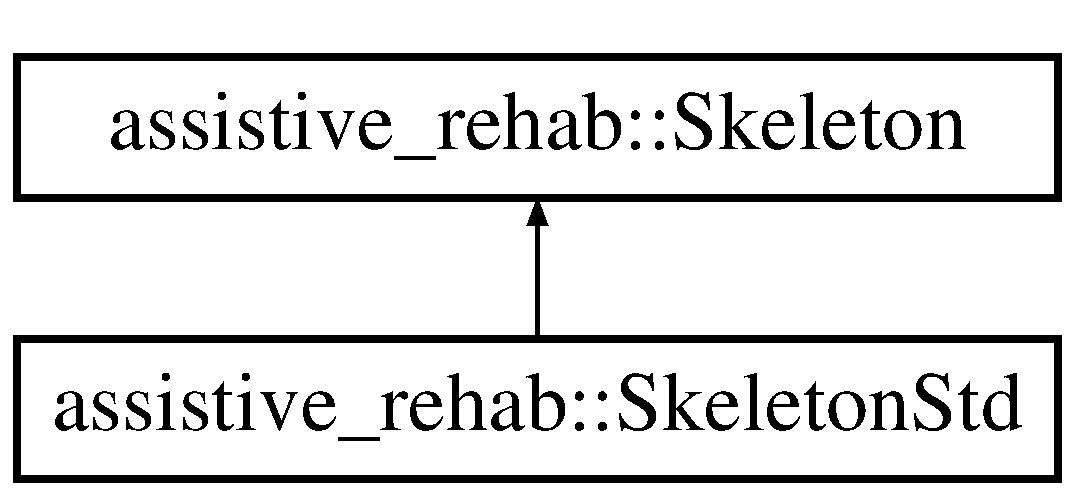
\includegraphics[height=2.000000cm]{classassistive__rehab_1_1SkeletonStd}
\end{center}
\end{figure}
\subsection*{Public Member Functions}
\begin{DoxyCompactItemize}
\item 
\mbox{\label{classassistive__rehab_1_1SkeletonStd_ae383ac2b515aa5774b010afc22856360}} 
\hyperlink{classassistive__rehab_1_1SkeletonStd_ae383ac2b515aa5774b010afc22856360}{Skeleton\+Std} ()
\begin{DoxyCompactList}\small\item\em Default constructor. \end{DoxyCompactList}\item 
bool \hyperlink{classassistive__rehab_1_1SkeletonStd_a5769bc6fd407118c866b57b869d672ca}{update\+\_\+planes} () override
\begin{DoxyCompactList}\small\item\em Update skeleton planes. \end{DoxyCompactList}\item 
const std\+::string \& \hyperlink{classassistive__rehab_1_1Skeleton_a4efc4844bd2b185f1080ee52ab69cb04}{get\+Type} () const
\begin{DoxyCompactList}\small\item\em Return a reference to the type of the skeleton. \end{DoxyCompactList}\item 
void \hyperlink{classassistive__rehab_1_1Skeleton_ae1c830e3d9a0ba692e5ae297caa52a82}{set\+Tag} (const std\+::string \&\hyperlink{classassistive__rehab_1_1Skeleton_a3d1ce5280300e012826948dc4383c2cb}{tag})
\begin{DoxyCompactList}\small\item\em Set the tag of the skeleton. \end{DoxyCompactList}\item 
const std\+::string \& \hyperlink{classassistive__rehab_1_1Skeleton_a185654045d5e43b3853cdb8fdd676da6}{get\+Tag} () const
\begin{DoxyCompactList}\small\item\em Return a reference to the tag of the skeleton. \end{DoxyCompactList}\item 
bool \hyperlink{classassistive__rehab_1_1Skeleton_a3486cbd7f59e75c1d9ef26cbc05bb72f}{set\+Transformation} (const yarp\+::sig\+::\+Matrix \&\hyperlink{classassistive__rehab_1_1Skeleton_a358a1c5eb23a562f8558ff8d43583ef7}{T})
\begin{DoxyCompactList}\small\item\em Set a new transformation matrix of the skeleton. \end{DoxyCompactList}\item 
const yarp\+::sig\+::\+Matrix \& \hyperlink{classassistive__rehab_1_1Skeleton_a2bdcc0d686a5a232aa2c07528cf2e647}{get\+Transformation} () const
\begin{DoxyCompactList}\small\item\em Retrieve the transformation matrix of the skeleton. \end{DoxyCompactList}\item 
bool \hyperlink{classassistive__rehab_1_1Skeleton_ab3bd697f48ea69cfdc5ff7574c19041f}{set\+Coronal} (const yarp\+::sig\+::\+Vector \&\hyperlink{classassistive__rehab_1_1Skeleton_ad042a7e60e6d72cc87b06c5fb0bdfae2}{coronal})
\begin{DoxyCompactList}\small\item\em Set a new coronal plane to the skeleton. \end{DoxyCompactList}\item 
bool \hyperlink{classassistive__rehab_1_1Skeleton_af92fdb0e3eb88a0b1dedd5038e2c6eb7}{set\+Sagittal} (const yarp\+::sig\+::\+Vector \&\hyperlink{classassistive__rehab_1_1Skeleton_a72d6ccb619619e77a17258b08496a972}{sagittal})
\begin{DoxyCompactList}\small\item\em Set a new sagittal plane to the skeleton. \end{DoxyCompactList}\item 
bool \hyperlink{classassistive__rehab_1_1Skeleton_a1aeba05a17363afc08c30397d17375df}{set\+Transverse} (const yarp\+::sig\+::\+Vector \&\hyperlink{classassistive__rehab_1_1Skeleton_ab8a9bf9297f520e8de801248e0b8d2dd}{transverse})
\begin{DoxyCompactList}\small\item\em Set a new transverse plane to the skeleton. \end{DoxyCompactList}\item 
yarp\+::sig\+::\+Vector \hyperlink{classassistive__rehab_1_1Skeleton_aa241a0ac93a9ead198f985073c8935eb}{get\+Coronal} () const
\begin{DoxyCompactList}\small\item\em Retrieve the coronal plane of the skeleton. \end{DoxyCompactList}\item 
yarp\+::sig\+::\+Vector \hyperlink{classassistive__rehab_1_1Skeleton_a83133fabc903ddd4e54edf59df977167}{get\+Sagittal} () const
\begin{DoxyCompactList}\small\item\em Retrieve the sagittal plane of the skeleton. \end{DoxyCompactList}\item 
yarp\+::sig\+::\+Vector \hyperlink{classassistive__rehab_1_1Skeleton_a35c3cdea575eb474a2cb8e0186011cff}{get\+Transverse} () const
\begin{DoxyCompactList}\small\item\em Retrieve the transverse plane of the skeleton. \end{DoxyCompactList}\item 
double \hyperlink{classassistive__rehab_1_1Skeleton_acda9030cd2ed3ad92697418a5e2cff7c}{get\+Max\+Path} () const
\begin{DoxyCompactList}\small\item\em Retrieve the skeleton\textquotesingle{}s maximum path. \end{DoxyCompactList}\item 
virtual yarp\+::os\+::\+Property \hyperlink{classassistive__rehab_1_1Skeleton_ad58ea53a165abc3f39a3c46594f0560f}{to\+Property} ()
\begin{DoxyCompactList}\small\item\em Export the skeleton structure as a property. \end{DoxyCompactList}\item 
virtual void \hyperlink{classassistive__rehab_1_1Skeleton_ac844f66503de87859833056dc33a835b}{from\+Property} (const yarp\+::os\+::\+Property \&prop)
\begin{DoxyCompactList}\small\item\em Import the skeleton structure from its properties. \end{DoxyCompactList}\item 
unsigned int \hyperlink{classassistive__rehab_1_1Skeleton_ac5e5b98f2c9178f6e0def5033e27922f}{get\+Num\+Key\+Points} () const
\begin{DoxyCompactList}\small\item\em Retrieve the number of keypoints of the skeleton. \end{DoxyCompactList}\item 
int \hyperlink{classassistive__rehab_1_1Skeleton_a954bfa99e0dad997ca6d93495246d3f1}{get\+Num\+From\+Key} (const std\+::string \&\hyperlink{classassistive__rehab_1_1Skeleton_a3d1ce5280300e012826948dc4383c2cb}{tag}) const
\begin{DoxyCompactList}\small\item\em Retrieve the index of the keypoint from its tag. \end{DoxyCompactList}\item 
const \hyperlink{classassistive__rehab_1_1KeyPoint}{Key\+Point} $\ast$ \hyperlink{classassistive__rehab_1_1Skeleton_a3ecc7418af653c88e40d41bb379b7271}{operator\mbox{[}$\,$\mbox{]}} (const std\+::string \&\hyperlink{classassistive__rehab_1_1Skeleton_a3d1ce5280300e012826948dc4383c2cb}{tag}) const
\begin{DoxyCompactList}\small\item\em Keypoint access. \end{DoxyCompactList}\item 
const \hyperlink{classassistive__rehab_1_1KeyPoint}{Key\+Point} $\ast$ \hyperlink{classassistive__rehab_1_1Skeleton_a0692ab89f16b0914b9ca9e0d4a07e52c}{operator\mbox{[}$\,$\mbox{]}} (const unsigned int i) const
\begin{DoxyCompactList}\small\item\em Keypoint access. \end{DoxyCompactList}\item 
\mbox{\label{classassistive__rehab_1_1Skeleton_a1ba2ba229331f7966ff1bce10c776d99}} 
virtual void \hyperlink{classassistive__rehab_1_1Skeleton_a1ba2ba229331f7966ff1bce10c776d99}{update} ()
\begin{DoxyCompactList}\small\item\em Update skeleton. \end{DoxyCompactList}\item 
virtual void \hyperlink{classassistive__rehab_1_1Skeleton_adbb387558eac21173b7c82cb43acd603}{update} (const std\+::vector$<$ yarp\+::sig\+::\+Vector $>$ \&ordered)
\begin{DoxyCompactList}\small\item\em Update skeleton from ordered list. \end{DoxyCompactList}\item 
virtual void \hyperlink{classassistive__rehab_1_1Skeleton_ab9642d6621d0a2b189c020f4d7695b14}{update} (const std\+::vector$<$ std\+::pair$<$ std\+::string, yarp\+::sig\+::\+Vector $>$$>$ \&unordered)
\begin{DoxyCompactList}\small\item\em Update skeleton from unordered list. \end{DoxyCompactList}\item 
virtual void \hyperlink{classassistive__rehab_1_1Skeleton_ae3346b2f363e1812fdc88e59d1f7bf7d}{update} (const yarp\+::os\+::\+Property \&prop)
\begin{DoxyCompactList}\small\item\em Update skeleton from properties. \end{DoxyCompactList}\item 
virtual void \hyperlink{classassistive__rehab_1_1Skeleton_a20d9eb5aecd6dccfa7e049bb932a6cef}{update\+\_\+withpixels} (const std\+::vector$<$ std\+::pair$<$ yarp\+::sig\+::\+Vector, yarp\+::sig\+::\+Vector $>$$>$ \&ordered)
\begin{DoxyCompactList}\small\item\em Update skeleton from ordered list. \end{DoxyCompactList}\item 
virtual void \hyperlink{classassistive__rehab_1_1Skeleton_a36e9dfd4910120025e40ccc3d03c0e01}{update\+\_\+withpixels} (const std\+::vector$<$ std\+::pair$<$ std\+::string, std\+::pair$<$ yarp\+::sig\+::\+Vector, yarp\+::sig\+::\+Vector $>$$>$$>$ \&unordered)
\begin{DoxyCompactList}\small\item\em Update skeleton from unordered list. \end{DoxyCompactList}\item 
virtual std\+::vector$<$ yarp\+::sig\+::\+Vector $>$ \hyperlink{classassistive__rehab_1_1Skeleton_a9c56f7f9e243ae2c4c3fef6dbb051dc2}{get\+\_\+ordered} () const
\begin{DoxyCompactList}\small\item\em Retrieve the ordered list of keypoints. \end{DoxyCompactList}\item 
virtual std\+::vector$<$ std\+::pair$<$ std\+::string, yarp\+::sig\+::\+Vector $>$ $>$ \hyperlink{classassistive__rehab_1_1Skeleton_a7b9f01b2b0f5450920335347c5861a2f}{get\+\_\+unordered} () const
\begin{DoxyCompactList}\small\item\em Retrieve the unordered list of keypoints. \end{DoxyCompactList}\item 
virtual std\+::vector$<$ std\+::pair$<$ yarp\+::sig\+::\+Vector, yarp\+::sig\+::\+Vector $>$ $>$ \hyperlink{classassistive__rehab_1_1Skeleton_a270506cde494cb4261c7892edb46ce53}{get\+\_\+ordered\+\_\+withpixels} () const
\begin{DoxyCompactList}\small\item\em Retrieve the ordered list of keypoints. \end{DoxyCompactList}\item 
virtual std\+::vector$<$ std\+::pair$<$ std\+::string, std\+::pair$<$ yarp\+::sig\+::\+Vector, yarp\+::sig\+::\+Vector $>$ $>$ $>$ \hyperlink{classassistive__rehab_1_1Skeleton_a513a3dc56d55a7b10b256378ae63c6c7}{get\+\_\+unordered\+\_\+withpixels} () const
\begin{DoxyCompactList}\small\item\em Retrieve the unordered list of keypoints. \end{DoxyCompactList}\item 
void \hyperlink{classassistive__rehab_1_1Skeleton_a7753cc8d2b43e27eaf7bf9ef640a99cb}{normalize} (const double n=1.\+0)
\begin{DoxyCompactList}\small\item\em Normalize skeleton in order to have unitary/desired distance among keypoints. \end{DoxyCompactList}\item 
void \hyperlink{classassistive__rehab_1_1Skeleton_a21fded128e2240e4dd507030b7386670}{scale} (const double s)
\begin{DoxyCompactList}\small\item\em Rescale skeleton. \end{DoxyCompactList}\item 
\mbox{\label{classassistive__rehab_1_1Skeleton_a58289ea0ba49220afac3e8d7128493b4}} 
void \hyperlink{classassistive__rehab_1_1Skeleton_a58289ea0ba49220afac3e8d7128493b4}{print} (std\+::ostream \&os=std\+::cout) const
\begin{DoxyCompactList}\small\item\em Print skeleton information. \end{DoxyCompactList}\end{DoxyCompactItemize}
\subsection*{Protected Member Functions}
\begin{DoxyCompactItemize}
\item 
\mbox{\label{classassistive__rehab_1_1Skeleton_ae448d21825bfd36eccb328d16fef995a}} 
yarp\+::os\+::\+Property {\bfseries helper\+\_\+toproperty} (\hyperlink{classassistive__rehab_1_1KeyPoint}{Key\+Point} $\ast$k) const
\item 
\mbox{\label{classassistive__rehab_1_1Skeleton_a8e8fcac9b911ce9eaa0a97b81bffb357}} 
void {\bfseries helper\+\_\+fromproperty} (yarp\+::os\+::\+Bottle $\ast$prop, \hyperlink{classassistive__rehab_1_1KeyPoint}{Key\+Point} $\ast$parent)
\item 
\mbox{\label{classassistive__rehab_1_1Skeleton_a8b1fa988e848ef1fc06439be8eaa19a4}} 
void {\bfseries helper\+\_\+updatefromproperty} (yarp\+::os\+::\+Bottle $\ast$prop)
\item 
\mbox{\label{classassistive__rehab_1_1Skeleton_a574ad07752a2a59ea765e10282998bb4}} 
void {\bfseries helper\+\_\+normalize} (\hyperlink{classassistive__rehab_1_1KeyPoint}{Key\+Point} $\ast$k, const std\+::vector$<$ yarp\+::sig\+::\+Vector $>$ \&helperpoints, const double n)
\item 
\mbox{\label{classassistive__rehab_1_1Skeleton_aefdf8624092fcc2b5458b0be108da01a}} 
void {\bfseries helper\+\_\+scale} (\hyperlink{classassistive__rehab_1_1KeyPoint}{Key\+Point} $\ast$k, const std\+::vector$<$ yarp\+::sig\+::\+Vector $>$ \&helperpoints, const double s)
\item 
\mbox{\label{classassistive__rehab_1_1Skeleton_a66ea19f4fbec2b654e394686180abf43}} 
double {\bfseries helper\+\_\+getmaxpath} (\hyperlink{classassistive__rehab_1_1KeyPoint}{Key\+Point} $\ast$k, std\+::vector$<$ bool $>$ \&visited) const
\end{DoxyCompactItemize}
\subsection*{Protected Attributes}
\begin{DoxyCompactItemize}
\item 
\mbox{\label{classassistive__rehab_1_1Skeleton_a679b826030f01f307d938e583f27d23b}} 
std\+::string \hyperlink{classassistive__rehab_1_1Skeleton_a679b826030f01f307d938e583f27d23b}{type}
\begin{DoxyCompactList}\small\item\em skeleton\textquotesingle{}s type (\char`\"{}assistive\+\_\+rehab\+::\+Skeleton\+Std\char`\"{}) \end{DoxyCompactList}\item 
\mbox{\label{classassistive__rehab_1_1Skeleton_a3d1ce5280300e012826948dc4383c2cb}} 
std\+::string \hyperlink{classassistive__rehab_1_1Skeleton_a3d1ce5280300e012826948dc4383c2cb}{tag}
\begin{DoxyCompactList}\small\item\em skeleton\textquotesingle{}s tag \end{DoxyCompactList}\item 
\mbox{\label{classassistive__rehab_1_1Skeleton_a5f61fbdd10430985cd6754e182226787}} 
std\+::vector$<$ \hyperlink{classassistive__rehab_1_1KeyPoint}{Key\+Point} $\ast$ $>$ \hyperlink{classassistive__rehab_1_1Skeleton_a5f61fbdd10430985cd6754e182226787}{keypoints}
\begin{DoxyCompactList}\small\item\em vector of pointer to \hyperlink{classassistive__rehab_1_1KeyPoint}{Key\+Point} \end{DoxyCompactList}\item 
\mbox{\label{classassistive__rehab_1_1Skeleton_ada4d4b327f1f71520e62e42db9d4c656}} 
std\+::unordered\+\_\+map$<$ std\+::string, \hyperlink{classassistive__rehab_1_1KeyPoint}{Key\+Point} $\ast$ $>$ \hyperlink{classassistive__rehab_1_1Skeleton_ada4d4b327f1f71520e62e42db9d4c656}{tag2key}
\begin{DoxyCompactList}\small\item\em map associating a tag to a pointer to a \hyperlink{classassistive__rehab_1_1KeyPoint}{Key\+Point} \end{DoxyCompactList}\item 
\mbox{\label{classassistive__rehab_1_1Skeleton_a4b1c3607cabb58053e4c367015e98e28}} 
std\+::unordered\+\_\+map$<$ \hyperlink{classassistive__rehab_1_1KeyPoint}{Key\+Point} $\ast$, unsigned int $>$ \hyperlink{classassistive__rehab_1_1Skeleton_a4b1c3607cabb58053e4c367015e98e28}{key2id}
\begin{DoxyCompactList}\small\item\em map associating a pointer to a \hyperlink{classassistive__rehab_1_1KeyPoint}{Key\+Point} to an index \end{DoxyCompactList}\item 
\mbox{\label{classassistive__rehab_1_1Skeleton_a358a1c5eb23a562f8558ff8d43583ef7}} 
yarp\+::sig\+::\+Matrix \hyperlink{classassistive__rehab_1_1Skeleton_a358a1c5eb23a562f8558ff8d43583ef7}{T}
\begin{DoxyCompactList}\small\item\em transformation matrix \end{DoxyCompactList}\item 
\mbox{\label{classassistive__rehab_1_1Skeleton_ad042a7e60e6d72cc87b06c5fb0bdfae2}} 
yarp\+::sig\+::\+Vector \hyperlink{classassistive__rehab_1_1Skeleton_ad042a7e60e6d72cc87b06c5fb0bdfae2}{coronal}
\begin{DoxyCompactList}\small\item\em vector containing the normal to the coronal plane \end{DoxyCompactList}\item 
\mbox{\label{classassistive__rehab_1_1Skeleton_a72d6ccb619619e77a17258b08496a972}} 
yarp\+::sig\+::\+Vector \hyperlink{classassistive__rehab_1_1Skeleton_a72d6ccb619619e77a17258b08496a972}{sagittal}
\begin{DoxyCompactList}\small\item\em vector containing the normal to the sagittal plane \end{DoxyCompactList}\item 
\mbox{\label{classassistive__rehab_1_1Skeleton_ab8a9bf9297f520e8de801248e0b8d2dd}} 
yarp\+::sig\+::\+Vector \hyperlink{classassistive__rehab_1_1Skeleton_ab8a9bf9297f520e8de801248e0b8d2dd}{transverse}
\begin{DoxyCompactList}\small\item\em vector containing the normal to the transverse plane \end{DoxyCompactList}\end{DoxyCompactItemize}


\subsection{Detailed Description}
Basic class for skeleton standard. 

Definition at line 528 of file skeleton.\+h.



\subsection{Member Function Documentation}
\mbox{\label{classassistive__rehab_1_1Skeleton_ac844f66503de87859833056dc33a835b}} 
\index{assistive\+\_\+rehab\+::\+Skeleton\+Std@{assistive\+\_\+rehab\+::\+Skeleton\+Std}!from\+Property@{from\+Property}}
\index{from\+Property@{from\+Property}!assistive\+\_\+rehab\+::\+Skeleton\+Std@{assistive\+\_\+rehab\+::\+Skeleton\+Std}}
\subsubsection{\texorpdfstring{from\+Property()}{fromProperty()}}
{\footnotesize\ttfamily void Skeleton\+::from\+Property (\begin{DoxyParamCaption}\item[{const yarp\+::os\+::\+Property \&}]{prop }\end{DoxyParamCaption})\hspace{0.3cm}{\ttfamily [virtual]}, {\ttfamily [inherited]}}



Import the skeleton structure from its properties. 


\begin{DoxyParams}{Parameters}
{\em prop} & Property object containing the properties of a skeleton.\\
\hline
\end{DoxyParams}
Available properties are\+:
\begin{DoxyItemize}
\item type\+: string containing skeleton\textquotesingle{}s type (\char`\"{}assistive\+\_\+rehab\+::\+Skeleton\+Std\char`\"{}).
\item tag\+: string containing skeleton\textquotesingle{}s tag.
\item transformation\+: 4 x 4 skeleton\textquotesingle{}s roto-\/translation matrix.
\item coronal\+: vector containing skeleton\textquotesingle{}s coronal plane.
\item sagittal\+: vector containing skeleton\textquotesingle{}s sagittal plane.
\item transverse\+: vector containing skeleton\textquotesingle{}s transverse plane.
\item skeleton\+: list containing keypoints with the following subproperties\+:
\begin{DoxyItemize}
\item tag\+: string containing keypoint\textquotesingle{}s tag.
\item status\+: string containing keypoint\textquotesingle{}s status (updated or stale).
\item position\+: vector containing keypoint\textquotesingle{}s camera coordinates x,y,z.
\item pixel\+: vector containing keypoint\textquotesingle{}s image coordinates u,v.
\item child\+: list containing keypoint\textquotesingle{}s child, specified as position, status, tag. 
\end{DoxyItemize}
\end{DoxyItemize}

Definition at line 400 of file skeleton.\+cpp.



Referenced by update\+\_\+planes().


\begin{DoxyCode}
401 \{
402     \textcolor{keywordflow}{for} (\textcolor{keyword}{auto} &k:keypoints)
403         \textcolor{keyword}{delete} k;
404 
405     keypoints.clear();
406     tag2key.clear();
407     key2id.clear();
408 
409     tag=prop.check(\textcolor{stringliteral}{"tag"},Value(\textcolor{stringliteral}{""})).asString();
410     \textcolor{keywordflow}{if} (prop.check(\textcolor{stringliteral}{"transformation"}))
411     \{
412         \textcolor{keywordflow}{if} (Bottle *b=prop.find(\textcolor{stringliteral}{"transformation"}).asList())
413             b->write(T);
414     \}
415     \textcolor{keywordflow}{else}
416         T=eye(4,4);
417 
418     coronal=sagittal=transverse=zeros(3);
419     \textcolor{keywordflow}{if} (prop.check(\textcolor{stringliteral}{"coronal"}))
420         \textcolor{keywordflow}{if} (Bottle *b=prop.find(\textcolor{stringliteral}{"coronal"}).asList())
421             b->write(coronal);
422     \textcolor{keywordflow}{if} (prop.check(\textcolor{stringliteral}{"sagittal"}))
423         \textcolor{keywordflow}{if} (Bottle *b=prop.find(\textcolor{stringliteral}{"sagittal"}).asList())
424             b->write(sagittal);
425     \textcolor{keywordflow}{if} (prop.check(\textcolor{stringliteral}{"transverse"}))
426         \textcolor{keywordflow}{if} (Bottle *b=prop.find(\textcolor{stringliteral}{"transverse"}).asList())
427             b->write(transverse);
428     helper\_fromproperty(prop.find(\textcolor{stringliteral}{"skeleton"}).asList(),\textcolor{keyword}{nullptr});
429 \}
\end{DoxyCode}
\mbox{\label{classassistive__rehab_1_1Skeleton_a9c56f7f9e243ae2c4c3fef6dbb051dc2}} 
\index{assistive\+\_\+rehab\+::\+Skeleton\+Std@{assistive\+\_\+rehab\+::\+Skeleton\+Std}!get\+\_\+ordered@{get\+\_\+ordered}}
\index{get\+\_\+ordered@{get\+\_\+ordered}!assistive\+\_\+rehab\+::\+Skeleton\+Std@{assistive\+\_\+rehab\+::\+Skeleton\+Std}}
\subsubsection{\texorpdfstring{get\+\_\+ordered()}{get\_ordered()}}
{\footnotesize\ttfamily vector$<$ Vector $>$ Skeleton\+::get\+\_\+ordered (\begin{DoxyParamCaption}{ }\end{DoxyParamCaption}) const\hspace{0.3cm}{\ttfamily [virtual]}, {\ttfamily [inherited]}}



Retrieve the ordered list of keypoints. 

\begin{DoxyReturn}{Returns}
vector containing the ordered list of keypoints, each specified as vector containing the x,y,z camera coordinates. 
\end{DoxyReturn}


Definition at line 581 of file skeleton.\+cpp.



References assistive\+\_\+rehab\+::\+Key\+Point\+::get\+Point().


\begin{DoxyCode}
582 \{
583     vector<Vector> ordered;
584     \textcolor{keywordflow}{for} (\textcolor{keyword}{auto} &k:keypoints)
585         ordered.push\_back(k->getPoint());
586     \textcolor{keywordflow}{return} ordered;
587 \}
\end{DoxyCode}
\mbox{\label{classassistive__rehab_1_1Skeleton_a270506cde494cb4261c7892edb46ce53}} 
\index{assistive\+\_\+rehab\+::\+Skeleton\+Std@{assistive\+\_\+rehab\+::\+Skeleton\+Std}!get\+\_\+ordered\+\_\+withpixels@{get\+\_\+ordered\+\_\+withpixels}}
\index{get\+\_\+ordered\+\_\+withpixels@{get\+\_\+ordered\+\_\+withpixels}!assistive\+\_\+rehab\+::\+Skeleton\+Std@{assistive\+\_\+rehab\+::\+Skeleton\+Std}}
\subsubsection{\texorpdfstring{get\+\_\+ordered\+\_\+withpixels()}{get\_ordered\_withpixels()}}
{\footnotesize\ttfamily vector$<$ pair$<$ Vector, Vector $>$ $>$ Skeleton\+::get\+\_\+ordered\+\_\+withpixels (\begin{DoxyParamCaption}{ }\end{DoxyParamCaption}) const\hspace{0.3cm}{\ttfamily [virtual]}, {\ttfamily [inherited]}}



Retrieve the ordered list of keypoints. 

\begin{DoxyReturn}{Returns}
vector containing the ordered list of keypoints, each specified as a pair of vectors with x,y,z and u,v coordinates. 
\end{DoxyReturn}


Definition at line 597 of file skeleton.\+cpp.



References assistive\+\_\+rehab\+::\+Key\+Point\+::get\+Pixel(), and assistive\+\_\+rehab\+::\+Key\+Point\+::get\+Point().


\begin{DoxyCode}
598 \{
599     vector<pair<Vector,Vector>> ordered;
600     \textcolor{keywordflow}{for} (\textcolor{keyword}{auto} &k:keypoints)
601         ordered.push\_back(make\_pair(k->getPoint(),k->getPixel()));
602     \textcolor{keywordflow}{return} ordered;
603 \}
\end{DoxyCode}
\mbox{\label{classassistive__rehab_1_1Skeleton_a7b9f01b2b0f5450920335347c5861a2f}} 
\index{assistive\+\_\+rehab\+::\+Skeleton\+Std@{assistive\+\_\+rehab\+::\+Skeleton\+Std}!get\+\_\+unordered@{get\+\_\+unordered}}
\index{get\+\_\+unordered@{get\+\_\+unordered}!assistive\+\_\+rehab\+::\+Skeleton\+Std@{assistive\+\_\+rehab\+::\+Skeleton\+Std}}
\subsubsection{\texorpdfstring{get\+\_\+unordered()}{get\_unordered()}}
{\footnotesize\ttfamily vector$<$ pair$<$ string, Vector $>$ $>$ Skeleton\+::get\+\_\+unordered (\begin{DoxyParamCaption}{ }\end{DoxyParamCaption}) const\hspace{0.3cm}{\ttfamily [virtual]}, {\ttfamily [inherited]}}



Retrieve the unordered list of keypoints. 

\begin{DoxyReturn}{Returns}
vector containing an unordered list of keypoints, each specified as pair which associates a string, containing the keypoint\textquotesingle{}s tag, and a vector, containing the x,y,z camera coordinates. 
\end{DoxyReturn}


Definition at line 589 of file skeleton.\+cpp.


\begin{DoxyCode}
590 \{
591     vector<pair<string,Vector>> unordered;
592     \textcolor{keywordflow}{for} (\textcolor{keyword}{auto} &it:tag2key)
593         unordered.push\_back(make\_pair(it.first,it.second->getPoint()));
594     \textcolor{keywordflow}{return} unordered;
595 \}
\end{DoxyCode}
\mbox{\label{classassistive__rehab_1_1Skeleton_a513a3dc56d55a7b10b256378ae63c6c7}} 
\index{assistive\+\_\+rehab\+::\+Skeleton\+Std@{assistive\+\_\+rehab\+::\+Skeleton\+Std}!get\+\_\+unordered\+\_\+withpixels@{get\+\_\+unordered\+\_\+withpixels}}
\index{get\+\_\+unordered\+\_\+withpixels@{get\+\_\+unordered\+\_\+withpixels}!assistive\+\_\+rehab\+::\+Skeleton\+Std@{assistive\+\_\+rehab\+::\+Skeleton\+Std}}
\subsubsection{\texorpdfstring{get\+\_\+unordered\+\_\+withpixels()}{get\_unordered\_withpixels()}}
{\footnotesize\ttfamily vector$<$ pair$<$ string, pair$<$ Vector, Vector $>$ $>$ $>$ Skeleton\+::get\+\_\+unordered\+\_\+withpixels (\begin{DoxyParamCaption}{ }\end{DoxyParamCaption}) const\hspace{0.3cm}{\ttfamily [virtual]}, {\ttfamily [inherited]}}



Retrieve the unordered list of keypoints. 

\begin{DoxyReturn}{Returns}
vector containing an unordered list of keypoints, each specified as pair that associates a string containing the keypoint\textquotesingle{}s tag to a pair of vectors of x,y,z and u,v coordinates. 
\end{DoxyReturn}


Definition at line 605 of file skeleton.\+cpp.


\begin{DoxyCode}
606 \{
607     vector<pair<string,pair<Vector,Vector>>> unordered;
608     \textcolor{keywordflow}{for} (\textcolor{keyword}{auto} &it:tag2key)
609         unordered.push\_back(make\_pair(it.first,make\_pair(it.second->getPoint(),it.second->getPixel())));
610     \textcolor{keywordflow}{return} unordered;
611 \}
\end{DoxyCode}
\mbox{\label{classassistive__rehab_1_1Skeleton_aa241a0ac93a9ead198f985073c8935eb}} 
\index{assistive\+\_\+rehab\+::\+Skeleton\+Std@{assistive\+\_\+rehab\+::\+Skeleton\+Std}!get\+Coronal@{get\+Coronal}}
\index{get\+Coronal@{get\+Coronal}!assistive\+\_\+rehab\+::\+Skeleton\+Std@{assistive\+\_\+rehab\+::\+Skeleton\+Std}}
\subsubsection{\texorpdfstring{get\+Coronal()}{getCoronal()}}
{\footnotesize\ttfamily Vector Skeleton\+::get\+Coronal (\begin{DoxyParamCaption}{ }\end{DoxyParamCaption}) const\hspace{0.3cm}{\ttfamily [inherited]}}



Retrieve the coronal plane of the skeleton. 

\begin{DoxyReturn}{Returns}
vector containing x,y,z coordinates of the normal to skeleton\textquotesingle{}s coronal plane. 
\end{DoxyReturn}


Definition at line 340 of file skeleton.\+cpp.


\begin{DoxyCode}
341 \{
342     \textcolor{keywordflow}{return} (T.submatrix(0,2,0,2)*coronal);
343 \}
\end{DoxyCode}
\mbox{\label{classassistive__rehab_1_1Skeleton_acda9030cd2ed3ad92697418a5e2cff7c}} 
\index{assistive\+\_\+rehab\+::\+Skeleton\+Std@{assistive\+\_\+rehab\+::\+Skeleton\+Std}!get\+Max\+Path@{get\+Max\+Path}}
\index{get\+Max\+Path@{get\+Max\+Path}!assistive\+\_\+rehab\+::\+Skeleton\+Std@{assistive\+\_\+rehab\+::\+Skeleton\+Std}}
\subsubsection{\texorpdfstring{get\+Max\+Path()}{getMaxPath()}}
{\footnotesize\ttfamily double Skeleton\+::get\+Max\+Path (\begin{DoxyParamCaption}{ }\end{DoxyParamCaption}) const\hspace{0.3cm}{\ttfamily [inherited]}}



Retrieve the skeleton\textquotesingle{}s maximum path. 

\begin{DoxyReturn}{Returns}
skeleton\textquotesingle{}s maximum path. 
\end{DoxyReturn}


Definition at line 355 of file skeleton.\+cpp.


\begin{DoxyCode}
356 \{
357     Vector paths(1,0.0);
358     \textcolor{keywordflow}{for} (\textcolor{keyword}{auto} &k:keypoints)
359     \{
360         vector<bool> visited(getNumKeyPoints(),\textcolor{keyword}{false});
361         paths.push\_back(helper\_getmaxpath(k,visited));
362     \}
363     \textcolor{keywordflow}{return} findMax(paths);
364 \}
\end{DoxyCode}
\mbox{\label{classassistive__rehab_1_1Skeleton_a954bfa99e0dad997ca6d93495246d3f1}} 
\index{assistive\+\_\+rehab\+::\+Skeleton\+Std@{assistive\+\_\+rehab\+::\+Skeleton\+Std}!get\+Num\+From\+Key@{get\+Num\+From\+Key}}
\index{get\+Num\+From\+Key@{get\+Num\+From\+Key}!assistive\+\_\+rehab\+::\+Skeleton\+Std@{assistive\+\_\+rehab\+::\+Skeleton\+Std}}
\subsubsection{\texorpdfstring{get\+Num\+From\+Key()}{getNumFromKey()}}
{\footnotesize\ttfamily int Skeleton\+::get\+Num\+From\+Key (\begin{DoxyParamCaption}\item[{const std\+::string \&}]{tag }\end{DoxyParamCaption}) const\hspace{0.3cm}{\ttfamily [inherited]}}



Retrieve the index of the keypoint from its tag. 


\begin{DoxyParams}{Parameters}
{\em tag} & string containing the keypoint\textquotesingle{}s tag. \\
\hline
\end{DoxyParams}
\begin{DoxyReturn}{Returns}
skeleton\textquotesingle{}s number of keypoints. 
\end{DoxyReturn}


Definition at line 431 of file skeleton.\+cpp.



References assistive\+\_\+rehab\+::\+Skeleton\+::operator\mbox{[}$\,$\mbox{]}().


\begin{DoxyCode}
432 \{
433     \textcolor{keyword}{auto} it1=tag2key.find(tag);
434     \textcolor{keywordflow}{if} (it1!=tag2key.end())
435     \{
436         \textcolor{keyword}{auto} it2=key2id.find(it1->second);
437         \textcolor{keywordflow}{if} (it2!=key2id.end())
438             \textcolor{keywordflow}{return} (\textcolor{keywordtype}{int})it2->second;
439     \}
440     \textcolor{keywordflow}{return} -1;
441 \}
\end{DoxyCode}
\mbox{\label{classassistive__rehab_1_1Skeleton_ac5e5b98f2c9178f6e0def5033e27922f}} 
\index{assistive\+\_\+rehab\+::\+Skeleton\+Std@{assistive\+\_\+rehab\+::\+Skeleton\+Std}!get\+Num\+Key\+Points@{get\+Num\+Key\+Points}}
\index{get\+Num\+Key\+Points@{get\+Num\+Key\+Points}!assistive\+\_\+rehab\+::\+Skeleton\+Std@{assistive\+\_\+rehab\+::\+Skeleton\+Std}}
\subsubsection{\texorpdfstring{get\+Num\+Key\+Points()}{getNumKeyPoints()}}
{\footnotesize\ttfamily unsigned int assistive\+\_\+rehab\+::\+Skeleton\+::get\+Num\+Key\+Points (\begin{DoxyParamCaption}{ }\end{DoxyParamCaption}) const\hspace{0.3cm}{\ttfamily [inline]}, {\ttfamily [inherited]}}



Retrieve the number of keypoints of the skeleton. 

\begin{DoxyReturn}{Returns}
skeleton\textquotesingle{}s number of keypoints. 
\end{DoxyReturn}


Definition at line 383 of file skeleton.\+h.


\begin{DoxyCode}
383 \{ \textcolor{keywordflow}{return} (\textcolor{keywordtype}{unsigned} \textcolor{keywordtype}{int})keypoints.size(); \}
\end{DoxyCode}
\mbox{\label{classassistive__rehab_1_1Skeleton_a83133fabc903ddd4e54edf59df977167}} 
\index{assistive\+\_\+rehab\+::\+Skeleton\+Std@{assistive\+\_\+rehab\+::\+Skeleton\+Std}!get\+Sagittal@{get\+Sagittal}}
\index{get\+Sagittal@{get\+Sagittal}!assistive\+\_\+rehab\+::\+Skeleton\+Std@{assistive\+\_\+rehab\+::\+Skeleton\+Std}}
\subsubsection{\texorpdfstring{get\+Sagittal()}{getSagittal()}}
{\footnotesize\ttfamily Vector Skeleton\+::get\+Sagittal (\begin{DoxyParamCaption}{ }\end{DoxyParamCaption}) const\hspace{0.3cm}{\ttfamily [inherited]}}



Retrieve the sagittal plane of the skeleton. 

\begin{DoxyReturn}{Returns}
vector containing the x,y,z coordinates of the normal skeleton\textquotesingle{}s sagittal plane. 
\end{DoxyReturn}


Definition at line 345 of file skeleton.\+cpp.


\begin{DoxyCode}
346 \{
347     \textcolor{keywordflow}{return} (T.submatrix(0,2,0,2)*sagittal);
348 \}
\end{DoxyCode}
\mbox{\label{classassistive__rehab_1_1Skeleton_a185654045d5e43b3853cdb8fdd676da6}} 
\index{assistive\+\_\+rehab\+::\+Skeleton\+Std@{assistive\+\_\+rehab\+::\+Skeleton\+Std}!get\+Tag@{get\+Tag}}
\index{get\+Tag@{get\+Tag}!assistive\+\_\+rehab\+::\+Skeleton\+Std@{assistive\+\_\+rehab\+::\+Skeleton\+Std}}
\subsubsection{\texorpdfstring{get\+Tag()}{getTag()}}
{\footnotesize\ttfamily const std\+::string\& assistive\+\_\+rehab\+::\+Skeleton\+::get\+Tag (\begin{DoxyParamCaption}{ }\end{DoxyParamCaption}) const\hspace{0.3cm}{\ttfamily [inline]}, {\ttfamily [inherited]}}



Return a reference to the tag of the skeleton. 

\begin{DoxyReturn}{Returns}
reference to a string containing the skeleton\textquotesingle{}s tag. 
\end{DoxyReturn}


Definition at line 278 of file skeleton.\+h.


\begin{DoxyCode}
278 \{ \textcolor{keywordflow}{return} tag; \}
\end{DoxyCode}
\mbox{\label{classassistive__rehab_1_1Skeleton_a2bdcc0d686a5a232aa2c07528cf2e647}} 
\index{assistive\+\_\+rehab\+::\+Skeleton\+Std@{assistive\+\_\+rehab\+::\+Skeleton\+Std}!get\+Transformation@{get\+Transformation}}
\index{get\+Transformation@{get\+Transformation}!assistive\+\_\+rehab\+::\+Skeleton\+Std@{assistive\+\_\+rehab\+::\+Skeleton\+Std}}
\subsubsection{\texorpdfstring{get\+Transformation()}{getTransformation()}}
{\footnotesize\ttfamily const yarp\+::sig\+::\+Matrix\& assistive\+\_\+rehab\+::\+Skeleton\+::get\+Transformation (\begin{DoxyParamCaption}{ }\end{DoxyParamCaption}) const\hspace{0.3cm}{\ttfamily [inline]}, {\ttfamily [inherited]}}



Retrieve the transformation matrix of the skeleton. 

\begin{DoxyReturn}{Returns}
reference to the skeleton\textquotesingle{}s transformation matrix. 
\end{DoxyReturn}
\begin{DoxyNote}{Note}
if the transformation matrix is the identity matrix, keypoints are defined with respect to the camera. 
\end{DoxyNote}


Definition at line 291 of file skeleton.\+h.


\begin{DoxyCode}
291 \{ \textcolor{keywordflow}{return} T; \}
\end{DoxyCode}
\mbox{\label{classassistive__rehab_1_1Skeleton_a35c3cdea575eb474a2cb8e0186011cff}} 
\index{assistive\+\_\+rehab\+::\+Skeleton\+Std@{assistive\+\_\+rehab\+::\+Skeleton\+Std}!get\+Transverse@{get\+Transverse}}
\index{get\+Transverse@{get\+Transverse}!assistive\+\_\+rehab\+::\+Skeleton\+Std@{assistive\+\_\+rehab\+::\+Skeleton\+Std}}
\subsubsection{\texorpdfstring{get\+Transverse()}{getTransverse()}}
{\footnotesize\ttfamily Vector Skeleton\+::get\+Transverse (\begin{DoxyParamCaption}{ }\end{DoxyParamCaption}) const\hspace{0.3cm}{\ttfamily [inherited]}}



Retrieve the transverse plane of the skeleton. 

\begin{DoxyReturn}{Returns}
vector containing the x,y,z coordinates of the normal skeleton\textquotesingle{}s sagittal plane. 
\end{DoxyReturn}


Definition at line 350 of file skeleton.\+cpp.


\begin{DoxyCode}
351 \{
352     \textcolor{keywordflow}{return} (T.submatrix(0,2,0,2)*transverse);
353 \}
\end{DoxyCode}
\mbox{\label{classassistive__rehab_1_1Skeleton_a4efc4844bd2b185f1080ee52ab69cb04}} 
\index{assistive\+\_\+rehab\+::\+Skeleton\+Std@{assistive\+\_\+rehab\+::\+Skeleton\+Std}!get\+Type@{get\+Type}}
\index{get\+Type@{get\+Type}!assistive\+\_\+rehab\+::\+Skeleton\+Std@{assistive\+\_\+rehab\+::\+Skeleton\+Std}}
\subsubsection{\texorpdfstring{get\+Type()}{getType()}}
{\footnotesize\ttfamily const std\+::string\& assistive\+\_\+rehab\+::\+Skeleton\+::get\+Type (\begin{DoxyParamCaption}{ }\end{DoxyParamCaption}) const\hspace{0.3cm}{\ttfamily [inline]}, {\ttfamily [inherited]}}



Return a reference to the type of the skeleton. 

\begin{DoxyReturn}{Returns}
reference to the skeleton\textquotesingle{}s type. 
\end{DoxyReturn}


Definition at line 266 of file skeleton.\+h.


\begin{DoxyCode}
266 \{ \textcolor{keywordflow}{return} type; \}
\end{DoxyCode}
\mbox{\label{classassistive__rehab_1_1Skeleton_a7753cc8d2b43e27eaf7bf9ef640a99cb}} 
\index{assistive\+\_\+rehab\+::\+Skeleton\+Std@{assistive\+\_\+rehab\+::\+Skeleton\+Std}!normalize@{normalize}}
\index{normalize@{normalize}!assistive\+\_\+rehab\+::\+Skeleton\+Std@{assistive\+\_\+rehab\+::\+Skeleton\+Std}}
\subsubsection{\texorpdfstring{normalize()}{normalize()}}
{\footnotesize\ttfamily void Skeleton\+::normalize (\begin{DoxyParamCaption}\item[{const double}]{n = {\ttfamily 1.0} }\end{DoxyParamCaption})\hspace{0.3cm}{\ttfamily [inherited]}}



Normalize skeleton in order to have unitary/desired distance among keypoints. 


\begin{DoxyParams}{Parameters}
{\em n} & double containing the normalization factor. \\
\hline
\end{DoxyParams}


Definition at line 613 of file skeleton.\+cpp.



References assistive\+\_\+rehab\+::\+Key\+Point\+::get\+Point().


\begin{DoxyCode}
614 \{
615     \textcolor{keywordflow}{if} (keypoints.size()>0)
616     \{
617         vector<Vector> helperpoints;
618         \textcolor{keywordflow}{for} (\textcolor{keyword}{auto} &k:keypoints)
619             helperpoints.push\_back(k->getPoint());
620         helper\_normalize(keypoints[0],helperpoints,n);
621     \}
622 \}
\end{DoxyCode}
\mbox{\label{classassistive__rehab_1_1Skeleton_a3ecc7418af653c88e40d41bb379b7271}} 
\index{assistive\+\_\+rehab\+::\+Skeleton\+Std@{assistive\+\_\+rehab\+::\+Skeleton\+Std}!operator\mbox{[}\mbox{]}@{operator[]}}
\index{operator\mbox{[}\mbox{]}@{operator[]}!assistive\+\_\+rehab\+::\+Skeleton\+Std@{assistive\+\_\+rehab\+::\+Skeleton\+Std}}
\subsubsection{\texorpdfstring{operator[]()}{operator[]()}\hspace{0.1cm}{\footnotesize\ttfamily [1/2]}}
{\footnotesize\ttfamily const \hyperlink{classassistive__rehab_1_1KeyPoint}{Key\+Point}$\ast$ assistive\+\_\+rehab\+::\+Skeleton\+::operator\mbox{[}$\,$\mbox{]} (\begin{DoxyParamCaption}\item[{const std\+::string \&}]{tag }\end{DoxyParamCaption}) const\hspace{0.3cm}{\ttfamily [inherited]}}



Keypoint access. 

Returns a pointer to the keypoint specified by its tag. 
\begin{DoxyParams}{Parameters}
{\em tag} & string containing the keypoint\textquotesingle{}s tag. \\
\hline
\end{DoxyParams}
\begin{DoxyReturn}{Returns}
a (const) pointer to the keypoint. 
\end{DoxyReturn}


Referenced by assistive\+\_\+rehab\+::\+Skeleton\+::get\+Num\+From\+Key().

\mbox{\label{classassistive__rehab_1_1Skeleton_a0692ab89f16b0914b9ca9e0d4a07e52c}} 
\index{assistive\+\_\+rehab\+::\+Skeleton\+Std@{assistive\+\_\+rehab\+::\+Skeleton\+Std}!operator\mbox{[}\mbox{]}@{operator[]}}
\index{operator\mbox{[}\mbox{]}@{operator[]}!assistive\+\_\+rehab\+::\+Skeleton\+Std@{assistive\+\_\+rehab\+::\+Skeleton\+Std}}
\subsubsection{\texorpdfstring{operator[]()}{operator[]()}\hspace{0.1cm}{\footnotesize\ttfamily [2/2]}}
{\footnotesize\ttfamily const \hyperlink{classassistive__rehab_1_1KeyPoint}{Key\+Point} $\ast$ Skeleton\+::operator\mbox{[}$\,$\mbox{]} (\begin{DoxyParamCaption}\item[{const unsigned int}]{i }\end{DoxyParamCaption}) const\hspace{0.3cm}{\ttfamily [inherited]}}



Keypoint access. 

Returns a pointer to the keypoint specified by its index. 
\begin{DoxyParams}{Parameters}
{\em i} & int containing the keypoint\textquotesingle{}s index. \\
\hline
\end{DoxyParams}
\begin{DoxyReturn}{Returns}
a (const) pointer to the keypoint. 
\end{DoxyReturn}


Definition at line 449 of file skeleton.\+cpp.


\begin{DoxyCode}
450 \{
451     \textcolor{keywordflow}{return} (i<keypoints.size())?keypoints[i]:\textcolor{keyword}{nullptr};
452 \}
\end{DoxyCode}
\mbox{\label{classassistive__rehab_1_1Skeleton_a21fded128e2240e4dd507030b7386670}} 
\index{assistive\+\_\+rehab\+::\+Skeleton\+Std@{assistive\+\_\+rehab\+::\+Skeleton\+Std}!scale@{scale}}
\index{scale@{scale}!assistive\+\_\+rehab\+::\+Skeleton\+Std@{assistive\+\_\+rehab\+::\+Skeleton\+Std}}
\subsubsection{\texorpdfstring{scale()}{scale()}}
{\footnotesize\ttfamily void Skeleton\+::scale (\begin{DoxyParamCaption}\item[{const double}]{s }\end{DoxyParamCaption})\hspace{0.3cm}{\ttfamily [inherited]}}



Rescale skeleton. 


\begin{DoxyParams}{Parameters}
{\em s} & double containing the scaling factor. \\
\hline
\end{DoxyParams}


Definition at line 624 of file skeleton.\+cpp.



References assistive\+\_\+rehab\+::\+Key\+Point\+::get\+Point().


\begin{DoxyCode}
625 \{
626     \textcolor{keywordflow}{if} (keypoints.size()>0)
627     \{
628         vector<Vector> helperpoints;
629         \textcolor{keywordflow}{for} (\textcolor{keyword}{auto} &k:keypoints)
630             helperpoints.push\_back(k->getPoint());
631         helper\_scale(keypoints[0],helperpoints,s);
632     \}
633 \}
\end{DoxyCode}
\mbox{\label{classassistive__rehab_1_1Skeleton_ab3bd697f48ea69cfdc5ff7574c19041f}} 
\index{assistive\+\_\+rehab\+::\+Skeleton\+Std@{assistive\+\_\+rehab\+::\+Skeleton\+Std}!set\+Coronal@{set\+Coronal}}
\index{set\+Coronal@{set\+Coronal}!assistive\+\_\+rehab\+::\+Skeleton\+Std@{assistive\+\_\+rehab\+::\+Skeleton\+Std}}
\subsubsection{\texorpdfstring{set\+Coronal()}{setCoronal()}}
{\footnotesize\ttfamily bool Skeleton\+::set\+Coronal (\begin{DoxyParamCaption}\item[{const yarp\+::sig\+::\+Vector \&}]{coronal }\end{DoxyParamCaption})\hspace{0.3cm}{\ttfamily [inherited]}}



Set a new coronal plane to the skeleton. 


\begin{DoxyParams}{Parameters}
{\em coronal} & vector containing the x,y,z coordinates of the normal to the desired plane. \\
\hline
\end{DoxyParams}


Definition at line 307 of file skeleton.\+cpp.


\begin{DoxyCode}
308 \{
309     \textcolor{keywordflow}{if} (coronal.length()>=3)
310     \{
311         this->coronal=coronal.subVector(0,2);
312         \textcolor{keywordflow}{return} \textcolor{keyword}{true};
313     \}
314     \textcolor{keywordflow}{else}
315         \textcolor{keywordflow}{return} \textcolor{keyword}{false};
316 \}
\end{DoxyCode}
\mbox{\label{classassistive__rehab_1_1Skeleton_af92fdb0e3eb88a0b1dedd5038e2c6eb7}} 
\index{assistive\+\_\+rehab\+::\+Skeleton\+Std@{assistive\+\_\+rehab\+::\+Skeleton\+Std}!set\+Sagittal@{set\+Sagittal}}
\index{set\+Sagittal@{set\+Sagittal}!assistive\+\_\+rehab\+::\+Skeleton\+Std@{assistive\+\_\+rehab\+::\+Skeleton\+Std}}
\subsubsection{\texorpdfstring{set\+Sagittal()}{setSagittal()}}
{\footnotesize\ttfamily bool Skeleton\+::set\+Sagittal (\begin{DoxyParamCaption}\item[{const yarp\+::sig\+::\+Vector \&}]{sagittal }\end{DoxyParamCaption})\hspace{0.3cm}{\ttfamily [inherited]}}



Set a new sagittal plane to the skeleton. 


\begin{DoxyParams}{Parameters}
{\em sagittal} & vector containing the x,y,z coordinates of the normal to the desired plane. \\
\hline
\end{DoxyParams}


Definition at line 318 of file skeleton.\+cpp.


\begin{DoxyCode}
319 \{
320     \textcolor{keywordflow}{if} (sagittal.length()>=3)
321     \{
322         this->sagittal=sagittal.subVector(0,2);
323         \textcolor{keywordflow}{return} \textcolor{keyword}{true};
324     \}
325     \textcolor{keywordflow}{else}
326         \textcolor{keywordflow}{return} \textcolor{keyword}{false};
327 \}
\end{DoxyCode}
\mbox{\label{classassistive__rehab_1_1Skeleton_ae1c830e3d9a0ba692e5ae297caa52a82}} 
\index{assistive\+\_\+rehab\+::\+Skeleton\+Std@{assistive\+\_\+rehab\+::\+Skeleton\+Std}!set\+Tag@{set\+Tag}}
\index{set\+Tag@{set\+Tag}!assistive\+\_\+rehab\+::\+Skeleton\+Std@{assistive\+\_\+rehab\+::\+Skeleton\+Std}}
\subsubsection{\texorpdfstring{set\+Tag()}{setTag()}}
{\footnotesize\ttfamily void assistive\+\_\+rehab\+::\+Skeleton\+::set\+Tag (\begin{DoxyParamCaption}\item[{const std\+::string \&}]{tag }\end{DoxyParamCaption})\hspace{0.3cm}{\ttfamily [inline]}, {\ttfamily [inherited]}}



Set the tag of the skeleton. 


\begin{DoxyParams}{Parameters}
{\em tag} & string containing the desired tag. \\
\hline
\end{DoxyParams}


Definition at line 272 of file skeleton.\+h.


\begin{DoxyCode}
272 \{ this->tag=tag; \}
\end{DoxyCode}
\mbox{\label{classassistive__rehab_1_1Skeleton_a3486cbd7f59e75c1d9ef26cbc05bb72f}} 
\index{assistive\+\_\+rehab\+::\+Skeleton\+Std@{assistive\+\_\+rehab\+::\+Skeleton\+Std}!set\+Transformation@{set\+Transformation}}
\index{set\+Transformation@{set\+Transformation}!assistive\+\_\+rehab\+::\+Skeleton\+Std@{assistive\+\_\+rehab\+::\+Skeleton\+Std}}
\subsubsection{\texorpdfstring{set\+Transformation()}{setTransformation()}}
{\footnotesize\ttfamily bool Skeleton\+::set\+Transformation (\begin{DoxyParamCaption}\item[{const yarp\+::sig\+::\+Matrix \&}]{T }\end{DoxyParamCaption})\hspace{0.3cm}{\ttfamily [inherited]}}



Set a new transformation matrix of the skeleton. 


\begin{DoxyParams}{Parameters}
{\em T} & matrix containing the desired transformation. \\
\hline
\end{DoxyParams}


Definition at line 296 of file skeleton.\+cpp.


\begin{DoxyCode}
297 \{
298     \textcolor{keywordflow}{if} ((T.rows()>=4) || (T.cols()>=4))
299     \{
300         this->T=T.submatrix(0,3,0,3);
301         \textcolor{keywordflow}{return} \textcolor{keyword}{true};
302     \}
303     \textcolor{keywordflow}{else}
304         \textcolor{keywordflow}{return} \textcolor{keyword}{false};
305 \}
\end{DoxyCode}
\mbox{\label{classassistive__rehab_1_1Skeleton_a1aeba05a17363afc08c30397d17375df}} 
\index{assistive\+\_\+rehab\+::\+Skeleton\+Std@{assistive\+\_\+rehab\+::\+Skeleton\+Std}!set\+Transverse@{set\+Transverse}}
\index{set\+Transverse@{set\+Transverse}!assistive\+\_\+rehab\+::\+Skeleton\+Std@{assistive\+\_\+rehab\+::\+Skeleton\+Std}}
\subsubsection{\texorpdfstring{set\+Transverse()}{setTransverse()}}
{\footnotesize\ttfamily bool Skeleton\+::set\+Transverse (\begin{DoxyParamCaption}\item[{const yarp\+::sig\+::\+Vector \&}]{transverse }\end{DoxyParamCaption})\hspace{0.3cm}{\ttfamily [inherited]}}



Set a new transverse plane to the skeleton. 


\begin{DoxyParams}{Parameters}
{\em transverse} & vector containing the x,y,z coordinates of the normal to the desired plane. \\
\hline
\end{DoxyParams}


Definition at line 329 of file skeleton.\+cpp.


\begin{DoxyCode}
330 \{
331     \textcolor{keywordflow}{if} (transverse.length()>=3)
332     \{
333         this->transverse=transverse.subVector(0,2);
334         \textcolor{keywordflow}{return} \textcolor{keyword}{true};
335     \}
336     \textcolor{keywordflow}{else}
337         \textcolor{keywordflow}{return} \textcolor{keyword}{false};
338 \}
\end{DoxyCode}
\mbox{\label{classassistive__rehab_1_1Skeleton_ad58ea53a165abc3f39a3c46594f0560f}} 
\index{assistive\+\_\+rehab\+::\+Skeleton\+Std@{assistive\+\_\+rehab\+::\+Skeleton\+Std}!to\+Property@{to\+Property}}
\index{to\+Property@{to\+Property}!assistive\+\_\+rehab\+::\+Skeleton\+Std@{assistive\+\_\+rehab\+::\+Skeleton\+Std}}
\subsubsection{\texorpdfstring{to\+Property()}{toProperty()}}
{\footnotesize\ttfamily Property Skeleton\+::to\+Property (\begin{DoxyParamCaption}{ }\end{DoxyParamCaption})\hspace{0.3cm}{\ttfamily [virtual]}, {\ttfamily [inherited]}}



Export the skeleton structure as a property. 

\begin{DoxyReturn}{Returns}
a Property object containing the properties of a skeleton.
\end{DoxyReturn}
Available properties are\+:
\begin{DoxyItemize}
\item type\+: string containing skeleton\textquotesingle{}s type (\char`\"{}assistive\+\_\+rehab\+::\+Skeleton\+Std\char`\"{}).
\item tag\+: string containing skeleton\textquotesingle{}s tag.
\item transformation\+: 4 x 4 skeleton\textquotesingle{}s roto-\/translation matrix.
\item coronal\+: vector containing skeleton\textquotesingle{}s coronal plane.
\item sagittal\+: vector containing skeleton\textquotesingle{}s sagittal plane.
\item transverse\+: vector containing skeleton\textquotesingle{}s transverse plane.
\item skeleton\+: list containing keypoints with the following subproperties\+:
\begin{DoxyItemize}
\item tag\+: string containing keypoint\textquotesingle{}s tag.
\item status\+: string containing keypoint\textquotesingle{}s status (updated or stale).
\item position\+: vector containing keypoint\textquotesingle{}s camera coordinates x,y,z.
\item pixel\+: vector containing keypoint\textquotesingle{}s image coordinates u,v.
\item child\+: list containing keypoint\textquotesingle{}s child, specified as position, status, tag. 
\end{DoxyItemize}
\end{DoxyItemize}

Definition at line 366 of file skeleton.\+cpp.


\begin{DoxyCode}
367 \{
368     Property prop;
369     prop.put(\textcolor{stringliteral}{"type"},type);
370     prop.put(\textcolor{stringliteral}{"tag"},tag);
371 
372     Bottle transformation;
373     transformation.addList().read(T);
374     prop.put(\textcolor{stringliteral}{"transformation"},transformation.get(0));
375 
376     Bottle plane;
377     plane.addList().read(coronal);
378     prop.put(\textcolor{stringliteral}{"coronal"},plane.get(0));
379 
380     plane.clear();
381     plane.addList().read(sagittal);
382     prop.put(\textcolor{stringliteral}{"sagittal"},plane.get(0));
383 
384     plane.clear();
385     plane.addList().read(transverse);
386     prop.put(\textcolor{stringliteral}{"transverse"},plane.get(0));
387 
388     Bottle skeleton;
389     Bottle &skeleton\_=skeleton.addList();
390     \textcolor{keywordflow}{if} (keypoints.size()>0)
391     \{
392         Property p=helper\_toproperty(keypoints[0]);
393         skeleton\_.addList().read(p);
394     \}
395     prop.put(\textcolor{stringliteral}{"skeleton"},skeleton.get(0));
396 
397     \textcolor{keywordflow}{return} prop;
398 \}
\end{DoxyCode}
\mbox{\label{classassistive__rehab_1_1Skeleton_adbb387558eac21173b7c82cb43acd603}} 
\index{assistive\+\_\+rehab\+::\+Skeleton\+Std@{assistive\+\_\+rehab\+::\+Skeleton\+Std}!update@{update}}
\index{update@{update}!assistive\+\_\+rehab\+::\+Skeleton\+Std@{assistive\+\_\+rehab\+::\+Skeleton\+Std}}
\subsubsection{\texorpdfstring{update()}{update()}\hspace{0.1cm}{\footnotesize\ttfamily [1/3]}}
{\footnotesize\ttfamily virtual void assistive\+\_\+rehab\+::\+Skeleton\+::update (\begin{DoxyParamCaption}\item[{const std\+::vector$<$ yarp\+::sig\+::\+Vector $>$ \&}]{ordered }\end{DoxyParamCaption})\hspace{0.3cm}{\ttfamily [virtual]}, {\ttfamily [inherited]}}



Update skeleton from ordered list. 


\begin{DoxyParams}{Parameters}
{\em ordered} & vector containing the ordered list of keypoints. The single keypoint is specified as vector containing the x,y,z coordinates. \\
\hline
\end{DoxyParams}
\mbox{\label{classassistive__rehab_1_1Skeleton_ab9642d6621d0a2b189c020f4d7695b14}} 
\index{assistive\+\_\+rehab\+::\+Skeleton\+Std@{assistive\+\_\+rehab\+::\+Skeleton\+Std}!update@{update}}
\index{update@{update}!assistive\+\_\+rehab\+::\+Skeleton\+Std@{assistive\+\_\+rehab\+::\+Skeleton\+Std}}
\subsubsection{\texorpdfstring{update()}{update()}\hspace{0.1cm}{\footnotesize\ttfamily [2/3]}}
{\footnotesize\ttfamily virtual void assistive\+\_\+rehab\+::\+Skeleton\+::update (\begin{DoxyParamCaption}\item[{const std\+::vector$<$ std\+::pair$<$ std\+::string, yarp\+::sig\+::\+Vector $>$$>$ \&}]{unordered }\end{DoxyParamCaption})\hspace{0.3cm}{\ttfamily [virtual]}, {\ttfamily [inherited]}}



Update skeleton from unordered list. 


\begin{DoxyParams}{Parameters}
{\em unordered} & vector containing an unordered list of keypoints. The single keypoint is specified as pair which associates a string, containing the keypoint\textquotesingle{}s tag, and a vector, containing the x,y,z coordinates. \\
\hline
\end{DoxyParams}
\mbox{\label{classassistive__rehab_1_1Skeleton_ae3346b2f363e1812fdc88e59d1f7bf7d}} 
\index{assistive\+\_\+rehab\+::\+Skeleton\+Std@{assistive\+\_\+rehab\+::\+Skeleton\+Std}!update@{update}}
\index{update@{update}!assistive\+\_\+rehab\+::\+Skeleton\+Std@{assistive\+\_\+rehab\+::\+Skeleton\+Std}}
\subsubsection{\texorpdfstring{update()}{update()}\hspace{0.1cm}{\footnotesize\ttfamily [3/3]}}
{\footnotesize\ttfamily virtual void assistive\+\_\+rehab\+::\+Skeleton\+::update (\begin{DoxyParamCaption}\item[{const yarp\+::os\+::\+Property \&}]{prop }\end{DoxyParamCaption})\hspace{0.3cm}{\ttfamily [virtual]}, {\ttfamily [inherited]}}



Update skeleton from properties. 


\begin{DoxyParams}{Parameters}
{\em prop} & a Property object containing skeleton information.\\
\hline
\end{DoxyParams}
Available properties are\+:
\begin{DoxyItemize}
\item type\+: string containing skeleton\textquotesingle{}s type (\char`\"{}assistive\+\_\+rehab\+::\+Skeleton\+Std\char`\"{}).
\item tag\+: string containing skeleton\textquotesingle{}s tag.
\item transformation\+: 4 x 4 skeleton\textquotesingle{}s roto-\/translation matrix.
\item coronal\+: vector containing skeleton\textquotesingle{}s coronal plane.
\item sagittal\+: vector containing skeleton\textquotesingle{}s sagittal plane.
\item transverse\+: vector containing skeleton\textquotesingle{}s transverse plane.
\item skeleton\+: list containing keypoints with the following subproperties\+:
\begin{DoxyItemize}
\item tag\+: string containing keypoint\textquotesingle{}s tag.
\item status\+: string containing keypoint\textquotesingle{}s status (updated or stale).
\item position\+: vector containing keypoint\textquotesingle{}s camera coordinates x,y,z.
\item pixel\+: vector containing keypoint\textquotesingle{}s image coordinates u,v.
\item child\+: list containing keypoint\textquotesingle{}s child, specified as position, status, tag. 
\end{DoxyItemize}
\end{DoxyItemize}\mbox{\label{classassistive__rehab_1_1SkeletonStd_a5769bc6fd407118c866b57b869d672ca}} 
\index{assistive\+\_\+rehab\+::\+Skeleton\+Std@{assistive\+\_\+rehab\+::\+Skeleton\+Std}!update\+\_\+planes@{update\+\_\+planes}}
\index{update\+\_\+planes@{update\+\_\+planes}!assistive\+\_\+rehab\+::\+Skeleton\+Std@{assistive\+\_\+rehab\+::\+Skeleton\+Std}}
\subsubsection{\texorpdfstring{update\+\_\+planes()}{update\_planes()}}
{\footnotesize\ttfamily bool Skeleton\+Std\+::update\+\_\+planes (\begin{DoxyParamCaption}{ }\end{DoxyParamCaption})\hspace{0.3cm}{\ttfamily [override]}, {\ttfamily [virtual]}}



Update skeleton planes. 

\begin{DoxyReturn}{Returns}
true/false on success/failure (failure occurs if not all planes are updated). 
\end{DoxyReturn}


Implements \hyperlink{classassistive__rehab_1_1Skeleton_af0ee2be195f804a9562cb184a2be0bad}{assistive\+\_\+rehab\+::\+Skeleton}.



Definition at line 767 of file skeleton.\+cpp.



References assistive\+\_\+rehab\+::\+Skeleton\+::from\+Property(), assistive\+\_\+rehab\+::\+Key\+Point\+::is\+Updated(), and assistive\+\_\+rehab\+::skeleton\+\_\+factory().


\begin{DoxyCode}
768 \{
769     \textcolor{keywordtype}{int} cnt=0;
770     \textcolor{keywordflow}{if} (tag2key[KeyPointTag::shoulder\_left]->isUpdated() &&
771         tag2key[KeyPointTag::shoulder\_right]->isUpdated())
772     \{
773         sagittal=tag2key[KeyPointTag::shoulder\_left]->getPoint()-
774                  tag2key[KeyPointTag::shoulder\_right]->getPoint();
775         \textcolor{keywordtype}{double} n=norm(sagittal);
776         \textcolor{keywordflow}{if} (n>0.0)
777             sagittal/=n;
778         cnt++;
779     \}
780 
781     \textcolor{keywordflow}{if} (tag2key[KeyPointTag::shoulder\_center]->isUpdated() &&
782         tag2key[KeyPointTag::hip\_center]->isUpdated())
783     \{
784         transverse=tag2key[KeyPointTag::shoulder\_center]->getPoint()-
785                    tag2key[KeyPointTag::hip\_center]->getPoint();
786         \textcolor{keywordtype}{double} n=norm(transverse);
787         \textcolor{keywordflow}{if} (n>0.0)
788             transverse/=n;
789         cnt++;
790     \}
791 
792     coronal=cross(sagittal,transverse);
793     \textcolor{keywordflow}{return} (cnt>=2);
794 \}
\end{DoxyCode}
\mbox{\label{classassistive__rehab_1_1Skeleton_a20d9eb5aecd6dccfa7e049bb932a6cef}} 
\index{assistive\+\_\+rehab\+::\+Skeleton\+Std@{assistive\+\_\+rehab\+::\+Skeleton\+Std}!update\+\_\+withpixels@{update\+\_\+withpixels}}
\index{update\+\_\+withpixels@{update\+\_\+withpixels}!assistive\+\_\+rehab\+::\+Skeleton\+Std@{assistive\+\_\+rehab\+::\+Skeleton\+Std}}
\subsubsection{\texorpdfstring{update\+\_\+withpixels()}{update\_withpixels()}\hspace{0.1cm}{\footnotesize\ttfamily [1/2]}}
{\footnotesize\ttfamily virtual void assistive\+\_\+rehab\+::\+Skeleton\+::update\+\_\+withpixels (\begin{DoxyParamCaption}\item[{const std\+::vector$<$ std\+::pair$<$ yarp\+::sig\+::\+Vector, yarp\+::sig\+::\+Vector $>$$>$ \&}]{ordered }\end{DoxyParamCaption})\hspace{0.3cm}{\ttfamily [virtual]}, {\ttfamily [inherited]}}



Update skeleton from ordered list. 


\begin{DoxyParams}{Parameters}
{\em ordered} & vector containing the ordered list of keypoints. The single keypoint is specified as a pair of a vector containing the x,y,z camera coordinates and a vector containing the u,v image coordinates. \\
\hline
\end{DoxyParams}


Referenced by assistive\+\_\+rehab\+::\+Skeleton\+::update().

\mbox{\label{classassistive__rehab_1_1Skeleton_a36e9dfd4910120025e40ccc3d03c0e01}} 
\index{assistive\+\_\+rehab\+::\+Skeleton\+Std@{assistive\+\_\+rehab\+::\+Skeleton\+Std}!update\+\_\+withpixels@{update\+\_\+withpixels}}
\index{update\+\_\+withpixels@{update\+\_\+withpixels}!assistive\+\_\+rehab\+::\+Skeleton\+Std@{assistive\+\_\+rehab\+::\+Skeleton\+Std}}
\subsubsection{\texorpdfstring{update\+\_\+withpixels()}{update\_withpixels()}\hspace{0.1cm}{\footnotesize\ttfamily [2/2]}}
{\footnotesize\ttfamily virtual void assistive\+\_\+rehab\+::\+Skeleton\+::update\+\_\+withpixels (\begin{DoxyParamCaption}\item[{const std\+::vector$<$ std\+::pair$<$ std\+::string, std\+::pair$<$ yarp\+::sig\+::\+Vector, yarp\+::sig\+::\+Vector $>$$>$$>$ \&}]{unordered }\end{DoxyParamCaption})\hspace{0.3cm}{\ttfamily [virtual]}, {\ttfamily [inherited]}}



Update skeleton from unordered list. 


\begin{DoxyParams}{Parameters}
{\em unordered} & vector containing an unordered list of keypoints. The single keypoint is specified as pair that associates a string containing the keypoint\textquotesingle{}s tag to a pair of vectors contianing x,y,z and u,v coordinates. \\
\hline
\end{DoxyParams}


The documentation for this class was generated from the following files\+:\begin{DoxyCompactItemize}
\item 
/home/vvasco/dev/robotology/assistive-\/rehab/lib/include/\+Assistive\+Rehab/skeleton.\+h\item 
/home/vvasco/dev/robotology/assistive-\/rehab/lib/src/\hyperlink{skeleton_8cpp}{skeleton.\+cpp}\end{DoxyCompactItemize}

\section{skeleton\+Viewer\+\_\+\+I\+DL Class Reference}
\label{classskeletonViewer__IDL}\index{skeleton\+Viewer\+\_\+\+I\+DL@{skeleton\+Viewer\+\_\+\+I\+DL}}


\hyperlink{classskeletonViewer__IDL}{skeleton\+Viewer\+\_\+\+I\+DL} I\+DL Interface to skeleton\+Viewer R\+PC services.  




{\ttfamily \#include $<$skeleton\+Viewer\+\_\+\+I\+D\+L.\+h$>$}



Inherits Wire.



Inherited by Viewer.

\subsection*{Public Member Functions}
\begin{DoxyCompactItemize}
\item 
virtual bool \hyperlink{classskeletonViewer__IDL_afdff1c47b3874a112c5fe601b2b9fac6}{set\+\_\+camera\+\_\+position} (const double x, const double y, const double z)
\begin{DoxyCompactList}\small\item\em Set the camera position in world coordinates. \end{DoxyCompactList}\item 
virtual bool \hyperlink{classskeletonViewer__IDL_a6b603079ea6fd21663de28091b9a1719}{set\+\_\+camera\+\_\+focalpoint} (const double x, const double y, const double z)
\begin{DoxyCompactList}\small\item\em Set the camera focal point in world coordinates. \end{DoxyCompactList}\item 
virtual bool \hyperlink{classskeletonViewer__IDL_addc168b73a8279fa6c146e4a7365cd77}{set\+\_\+camera\+\_\+viewup} (const double x, const double y, const double z)
\begin{DoxyCompactList}\small\item\em Set the camera view up direction in world coordinates. \end{DoxyCompactList}\item 
virtual bool \hyperlink{classskeletonViewer__IDL_ae893be656a21bfd75682fd4efb20a2d8}{create\+\_\+line} (const std\+::string \&name, const double x0, const double y0, const double z0, const double x1, const double y1, const double z1, const double r, const double g, const double b)
\begin{DoxyCompactList}\small\item\em Create a line. \end{DoxyCompactList}\item 
virtual bool \hyperlink{classskeletonViewer__IDL_a3a1f90f10689c4411e522d41d5d19908}{delete\+\_\+line} (const std\+::string \&name)
\begin{DoxyCompactList}\small\item\em Delete a line. \end{DoxyCompactList}\item 
\mbox{\label{classskeletonViewer__IDL_a970ce92704e75f8f8a4e663aace17436}} 
virtual std\+::vector$<$ std\+::string $>$ {\bfseries help} (const std\+::string \&function\+Name=\char`\"{}-\/-\/all\char`\"{})
\item 
\mbox{\label{classskeletonViewer__IDL_ae6e019ed8b536029c204defd60c7d63b}} 
bool {\bfseries read} (yarp\+::os\+::\+Connection\+Reader \&connection) override
\end{DoxyCompactItemize}


\subsection{Detailed Description}
\hyperlink{classskeletonViewer__IDL}{skeleton\+Viewer\+\_\+\+I\+DL} I\+DL Interface to skeleton\+Viewer R\+PC services. 

Definition at line 24 of file skeleton\+Viewer\+\_\+\+I\+D\+L.\+h.



\subsection{Member Function Documentation}
\mbox{\label{classskeletonViewer__IDL_ae893be656a21bfd75682fd4efb20a2d8}} 
\index{skeleton\+Viewer\+\_\+\+I\+DL@{skeleton\+Viewer\+\_\+\+I\+DL}!create\+\_\+line@{create\+\_\+line}}
\index{create\+\_\+line@{create\+\_\+line}!skeleton\+Viewer\+\_\+\+I\+DL@{skeleton\+Viewer\+\_\+\+I\+DL}}
\subsubsection{\texorpdfstring{create\+\_\+line()}{create\_line()}}
{\footnotesize\ttfamily virtual bool skeleton\+Viewer\+\_\+\+I\+D\+L\+::create\+\_\+line (\begin{DoxyParamCaption}\item[{const std\+::string \&}]{name,  }\item[{const double}]{x0,  }\item[{const double}]{y0,  }\item[{const double}]{z0,  }\item[{const double}]{x1,  }\item[{const double}]{y1,  }\item[{const double}]{z1,  }\item[{const double}]{r,  }\item[{const double}]{g,  }\item[{const double}]{b }\end{DoxyParamCaption})\hspace{0.3cm}{\ttfamily [virtual]}}



Create a line. 


\begin{DoxyParams}{Parameters}
{\em name} & is the name of the line. \\
\hline
{\em x0} & the x-\/coordinate of the line origin (meters). \\
\hline
{\em y0} & the y-\/coordinate of the line origin (meters). \\
\hline
{\em z0} & the z-\/coordinate of the line origin (meters). \\
\hline
{\em x1} & the x-\/coordinate of the line end (meters). \\
\hline
{\em y1} & the y-\/coordinate of the line end (meters). \\
\hline
{\em z1} & the z-\/coordinate of the line end (meters). \\
\hline
{\em r} & is the red channel of the line color \mbox{[}0,1\mbox{]}. \\
\hline
{\em g} & is the green channel of the line color \mbox{[}0,1\mbox{]}. \\
\hline
{\em b} & is the blue channel of the line color \mbox{[}0,1\mbox{]}. \\
\hline
\end{DoxyParams}
\begin{DoxyReturn}{Returns}
true/false on success/failure. 
\end{DoxyReturn}
\mbox{\label{classskeletonViewer__IDL_a3a1f90f10689c4411e522d41d5d19908}} 
\index{skeleton\+Viewer\+\_\+\+I\+DL@{skeleton\+Viewer\+\_\+\+I\+DL}!delete\+\_\+line@{delete\+\_\+line}}
\index{delete\+\_\+line@{delete\+\_\+line}!skeleton\+Viewer\+\_\+\+I\+DL@{skeleton\+Viewer\+\_\+\+I\+DL}}
\subsubsection{\texorpdfstring{delete\+\_\+line()}{delete\_line()}}
{\footnotesize\ttfamily virtual bool skeleton\+Viewer\+\_\+\+I\+D\+L\+::delete\+\_\+line (\begin{DoxyParamCaption}\item[{const std\+::string \&}]{name }\end{DoxyParamCaption})\hspace{0.3cm}{\ttfamily [virtual]}}



Delete a line. 


\begin{DoxyParams}{Parameters}
{\em name} & is the name of the line to delete. \\
\hline
\end{DoxyParams}
\begin{DoxyReturn}{Returns}
true/false on success/failure. 
\end{DoxyReturn}
\mbox{\label{classskeletonViewer__IDL_a6b603079ea6fd21663de28091b9a1719}} 
\index{skeleton\+Viewer\+\_\+\+I\+DL@{skeleton\+Viewer\+\_\+\+I\+DL}!set\+\_\+camera\+\_\+focalpoint@{set\+\_\+camera\+\_\+focalpoint}}
\index{set\+\_\+camera\+\_\+focalpoint@{set\+\_\+camera\+\_\+focalpoint}!skeleton\+Viewer\+\_\+\+I\+DL@{skeleton\+Viewer\+\_\+\+I\+DL}}
\subsubsection{\texorpdfstring{set\+\_\+camera\+\_\+focalpoint()}{set\_camera\_focalpoint()}}
{\footnotesize\ttfamily virtual bool skeleton\+Viewer\+\_\+\+I\+D\+L\+::set\+\_\+camera\+\_\+focalpoint (\begin{DoxyParamCaption}\item[{const double}]{x,  }\item[{const double}]{y,  }\item[{const double}]{z }\end{DoxyParamCaption})\hspace{0.3cm}{\ttfamily [virtual]}}



Set the camera focal point in world coordinates. 


\begin{DoxyParams}{Parameters}
{\em x} & is the x-\/coordinate (meters). \\
\hline
{\em y} & is the y-\/coordinate (meters). \\
\hline
{\em z} & is the z-\/coordinate (meters). \\
\hline
\end{DoxyParams}
\begin{DoxyReturn}{Returns}
true/false on success/failure. 
\end{DoxyReturn}
\mbox{\label{classskeletonViewer__IDL_afdff1c47b3874a112c5fe601b2b9fac6}} 
\index{skeleton\+Viewer\+\_\+\+I\+DL@{skeleton\+Viewer\+\_\+\+I\+DL}!set\+\_\+camera\+\_\+position@{set\+\_\+camera\+\_\+position}}
\index{set\+\_\+camera\+\_\+position@{set\+\_\+camera\+\_\+position}!skeleton\+Viewer\+\_\+\+I\+DL@{skeleton\+Viewer\+\_\+\+I\+DL}}
\subsubsection{\texorpdfstring{set\+\_\+camera\+\_\+position()}{set\_camera\_position()}}
{\footnotesize\ttfamily virtual bool skeleton\+Viewer\+\_\+\+I\+D\+L\+::set\+\_\+camera\+\_\+position (\begin{DoxyParamCaption}\item[{const double}]{x,  }\item[{const double}]{y,  }\item[{const double}]{z }\end{DoxyParamCaption})\hspace{0.3cm}{\ttfamily [virtual]}}



Set the camera position in world coordinates. 


\begin{DoxyParams}{Parameters}
{\em x} & is the x-\/coordinate (meters). \\
\hline
{\em y} & is the y-\/coordinate (meters). \\
\hline
{\em z} & is the z-\/coordinate (meters). \\
\hline
\end{DoxyParams}
\begin{DoxyReturn}{Returns}
true/false on success/failure. 
\end{DoxyReturn}
\mbox{\label{classskeletonViewer__IDL_addc168b73a8279fa6c146e4a7365cd77}} 
\index{skeleton\+Viewer\+\_\+\+I\+DL@{skeleton\+Viewer\+\_\+\+I\+DL}!set\+\_\+camera\+\_\+viewup@{set\+\_\+camera\+\_\+viewup}}
\index{set\+\_\+camera\+\_\+viewup@{set\+\_\+camera\+\_\+viewup}!skeleton\+Viewer\+\_\+\+I\+DL@{skeleton\+Viewer\+\_\+\+I\+DL}}
\subsubsection{\texorpdfstring{set\+\_\+camera\+\_\+viewup()}{set\_camera\_viewup()}}
{\footnotesize\ttfamily virtual bool skeleton\+Viewer\+\_\+\+I\+D\+L\+::set\+\_\+camera\+\_\+viewup (\begin{DoxyParamCaption}\item[{const double}]{x,  }\item[{const double}]{y,  }\item[{const double}]{z }\end{DoxyParamCaption})\hspace{0.3cm}{\ttfamily [virtual]}}



Set the camera view up direction in world coordinates. 


\begin{DoxyParams}{Parameters}
{\em x} & is the x-\/coordinate (meters). \\
\hline
{\em y} & is the y-\/coordinate (meters). \\
\hline
{\em z} & is the z-\/coordinate (meters). \\
\hline
\end{DoxyParams}
\begin{DoxyReturn}{Returns}
true/false on success/failure. 
\end{DoxyReturn}


The documentation for this class was generated from the following file\+:\begin{DoxyCompactItemize}
\item 
idl\+\_\+dox/skeleton\+Viewer\+\_\+\+I\+D\+L.\+h\end{DoxyCompactItemize}

\chapter{File Documentation}
\section{/home/vvasco/dev/robotology/assistive-\/rehab/lib/src/dtw.cpp File Reference}
\label{dtw_8cpp}\index{/home/vvasco/dev/robotology/assistive-\/rehab/lib/src/dtw.\+cpp@{/home/vvasco/dev/robotology/assistive-\/rehab/lib/src/dtw.\+cpp}}
{\ttfamily \#include $<$iostream$>$}\newline
{\ttfamily \#include $<$yarp/sig/all.\+h$>$}\newline
{\ttfamily \#include $<$yarp/math/\+Math.\+h$>$}\newline
{\ttfamily \#include \char`\"{}Assistive\+Rehab/dtw.\+h\char`\"{}}\newline


\subsection{Detailed Description}
\begin{DoxyAuthor}{Authors}
\+: Valentina Vasco \href{mailto:valentina.vasco@iit.it}{\tt valentina.\+vasco@iit.\+it} 
\end{DoxyAuthor}

\section{/home/vvasco/dev/robotology/assistive-\/rehab/lib/src/helpers.cpp File Reference}
\label{helpers_8cpp}\index{/home/vvasco/dev/robotology/assistive-\/rehab/lib/src/helpers.\+cpp@{/home/vvasco/dev/robotology/assistive-\/rehab/lib/src/helpers.\+cpp}}
{\ttfamily \#include $<$limits$>$}\newline
{\ttfamily \#include $<$utility$>$}\newline
{\ttfamily \#include $<$opencv2/opencv.\+hpp$>$}\newline
{\ttfamily \#include $<$yarp/cv/\+Cv.\+h$>$}\newline
{\ttfamily \#include \char`\"{}Assistive\+Rehab/helpers.\+h\char`\"{}}\newline


\subsection{Detailed Description}
\begin{DoxyAuthor}{Authors}
\+: Ugo Pattacini \href{mailto:ugo.pattacini@iit.it}{\tt ugo.\+pattacini@iit.\+it} 
\end{DoxyAuthor}

\section{/home/vvasco/dev/robotology/assistive-\/rehab/lib/src/skeleton.cpp File Reference}
\label{skeleton_8cpp}\index{/home/vvasco/dev/robotology/assistive-\/rehab/lib/src/skeleton.\+cpp@{/home/vvasco/dev/robotology/assistive-\/rehab/lib/src/skeleton.\+cpp}}
{\ttfamily \#include $<$algorithm$>$}\newline
{\ttfamily \#include $<$yarp/math/\+Math.\+h$>$}\newline
{\ttfamily \#include \char`\"{}Assistive\+Rehab/skeleton.\+h\char`\"{}}\newline


\subsection{Detailed Description}
\begin{DoxyAuthor}{Authors}
\+: Ugo Pattacini \href{mailto:ugo.pattacini@iit.it}{\tt ugo.\+pattacini@iit.\+it} 
\end{DoxyAuthor}

\section{/home/vvasco/dev/robotology/assistive-\/rehab/modules/motion\+Analyzer/include/\+Exercise.h File Reference}
\label{Exercise_8h}\index{/home/vvasco/dev/robotology/assistive-\/rehab/modules/motion\+Analyzer/include/\+Exercise.\+h@{/home/vvasco/dev/robotology/assistive-\/rehab/modules/motion\+Analyzer/include/\+Exercise.\+h}}
{\ttfamily \#include $<$Metric.\+h$>$}\newline
\subsection*{Variables}
\begin{DoxyCompactItemize}
\item 
\mbox{\label{Exercise_8h_ad3d299b4cbdcf9590a34383c9769552b}} 
const std\+::string {\bfseries Exercise\+Type\+::rehabilitation} =\char`\"{}rehabilitation\char`\"{}
\item 
\mbox{\label{Exercise_8h_a1b9417d7d699f4c9615ac6ca865c2b24}} 
const std\+::string {\bfseries Exercise\+Type\+::test} =\char`\"{}test\char`\"{}
\item 
\mbox{\label{Exercise_8h_a677cff5d00b858887bfc87459677f4c3}} 
const std\+::string {\bfseries Exercise\+Tag\+::abduction\+\_\+left} =\char`\"{}abduction\+\_\+left\char`\"{}
\item 
\mbox{\label{Exercise_8h_aa57cd043979311c1e1dfb6fe25c311e9}} 
const std\+::string {\bfseries Exercise\+Tag\+::internal\+\_\+rotation\+\_\+left} =\char`\"{}internal\+\_\+rotation\+\_\+left\char`\"{}
\item 
\mbox{\label{Exercise_8h_a85804e87dc5e4ce068563687f55eebe6}} 
const std\+::string {\bfseries Exercise\+Tag\+::external\+\_\+rotation\+\_\+left} =\char`\"{}external\+\_\+rotation\+\_\+left\char`\"{}
\item 
\mbox{\label{Exercise_8h_ae4590339042bcaf138b615ef43fd4ce0}} 
const std\+::string {\bfseries Exercise\+Tag\+::reaching\+\_\+left} =\char`\"{}reaching\+\_\+left\char`\"{}
\item 
\mbox{\label{Exercise_8h_a340ab8f95503666972bfff376c1f6627}} 
const std\+::string {\bfseries Exercise\+Tag\+::tug} =\char`\"{}tug\char`\"{}
\end{DoxyCompactItemize}


\subsection{Detailed Description}
\begin{DoxyAuthor}{Authors}
\+: Valentina Vasco \href{mailto:valentina.vasco@iit.it}{\tt valentina.\+vasco@iit.\+it} 
\end{DoxyAuthor}

\section{/home/vvasco/dev/robotology/assistive-\/rehab/modules/motion\+Analyzer/include/\+Manager.h File Reference}
\label{Manager_8h}\index{/home/vvasco/dev/robotology/assistive-\/rehab/modules/motion\+Analyzer/include/\+Manager.\+h@{/home/vvasco/dev/robotology/assistive-\/rehab/modules/motion\+Analyzer/include/\+Manager.\+h}}
{\ttfamily \#include $<$mutex$>$}\newline
{\ttfamily \#include $<$fstream$>$}\newline
{\ttfamily \#include $<$list$>$}\newline
{\ttfamily \#include $<$yarp/os/all.\+h$>$}\newline
{\ttfamily \#include $<$yarp/sig/\+Vector.\+h$>$}\newline
{\ttfamily \#include $<$yarp/sig/\+Matrix.\+h$>$}\newline
{\ttfamily \#include $<$Assistive\+Rehab/skeleton.\+h$>$}\newline
{\ttfamily \#include \char`\"{}Manager.\+h\char`\"{}}\newline
{\ttfamily \#include \char`\"{}Processor.\+h\char`\"{}}\newline
{\ttfamily \#include \char`\"{}Metric.\+h\char`\"{}}\newline
{\ttfamily \#include \char`\"{}Exercise.\+h\char`\"{}}\newline
{\ttfamily \#include \char`\"{}src/motion\+Analyzer\+\_\+\+I\+D\+L.\+h\char`\"{}}\newline
{\ttfamily \#include \char`\"{}matio.\+h\char`\"{}}\newline


\subsection{Detailed Description}
\begin{DoxyAuthor}{Authors}
\+: Valentina Vasco \href{mailto:valentina.vasco@iit.it}{\tt valentina.\+vasco@iit.\+it} 
\end{DoxyAuthor}

\section{/home/vvasco/dev/robotology/assistive-\/rehab/modules/motion\+Analyzer/include/\+Metric.h File Reference}
\label{Metric_8h}\index{/home/vvasco/dev/robotology/assistive-\/rehab/modules/motion\+Analyzer/include/\+Metric.\+h@{/home/vvasco/dev/robotology/assistive-\/rehab/modules/motion\+Analyzer/include/\+Metric.\+h}}
{\ttfamily \#include $<$iostream$>$}\newline
{\ttfamily \#include $<$map$>$}\newline
{\ttfamily \#include $<$yarp/os/all.\+h$>$}\newline
{\ttfamily \#include $<$yarp/sig/\+Vector.\+h$>$}\newline
{\ttfamily \#include $<$Assistive\+Rehab/skeleton.\+h$>$}\newline
\subsection*{Variables}
\begin{DoxyCompactItemize}
\item 
\mbox{\label{Metric_8h_a134a0ba35a0bfd473142dcba2fa0ac8f}} 
const std\+::string {\bfseries Metric\+Type\+::rom} =\char`\"{}R\+OM\char`\"{}
\item 
\mbox{\label{Metric_8h_ac4580e78dfaef7eb23d717bd230174e4}} 
const std\+::string {\bfseries Metric\+Type\+::end\+\_\+point} =\char`\"{}EP\char`\"{}
\item 
\mbox{\label{Metric_8h_a72bfe667eedeae0fa4a698a4450413d2}} 
const std\+::string {\bfseries Metric\+Type\+::step} =\char`\"{}step\char`\"{}
\end{DoxyCompactItemize}


\subsection{Detailed Description}
\begin{DoxyAuthor}{Authors}
\+: Valentina Vasco \href{mailto:valentina.vasco@iit.it}{\tt valentina.\+vasco@iit.\+it} 
\end{DoxyAuthor}

\section{/home/vvasco/dev/robotology/assistive-\/rehab/modules/motion\+Analyzer/include/\+Processor.h File Reference}
\label{Processor_8h}\index{/home/vvasco/dev/robotology/assistive-\/rehab/modules/motion\+Analyzer/include/\+Processor.\+h@{/home/vvasco/dev/robotology/assistive-\/rehab/modules/motion\+Analyzer/include/\+Processor.\+h}}
{\ttfamily \#include $<$iostream$>$}\newline
{\ttfamily \#include $<$map$>$}\newline
{\ttfamily \#include $<$cmath$>$}\newline
{\ttfamily \#include $<$fstream$>$}\newline
{\ttfamily \#include $<$yarp/sig/\+Matrix.\+h$>$}\newline
{\ttfamily \#include $<$yarp/math/\+Math.\+h$>$}\newline
{\ttfamily \#include $<$i\+Cub/ctrl/adapt\+Win\+Poly\+Estimator.\+h$>$}\newline
{\ttfamily \#include $<$i\+Cub/ctrl/filters.\+h$>$}\newline
{\ttfamily \#include $<$Assistive\+Rehab/skeleton.\+h$>$}\newline
{\ttfamily \#include \char`\"{}Metric.\+h\char`\"{}}\newline
\subsection*{Functions}
\begin{DoxyCompactItemize}
\item 
\mbox{\label{Processor_8h_a0ae4c67160d19584fcd102d4616a5bee}} 
Processor $\ast$ {\bfseries create\+Processor} (const std\+::string \&metric\+\_\+type, const Metric $\ast$metric\+\_\+)
\end{DoxyCompactItemize}


\subsection{Detailed Description}
\begin{DoxyAuthor}{Authors}
\+: Valentina Vasco \href{mailto:valentina.vasco@iit.it}{\tt valentina.\+vasco@iit.\+it} 
\end{DoxyAuthor}

\section{/home/vvasco/dev/robotology/assistive-\/rehab/modules/motion\+Analyzer/src/\+Exercise.cpp File Reference}
\label{Exercise_8cpp}\index{/home/vvasco/dev/robotology/assistive-\/rehab/modules/motion\+Analyzer/src/\+Exercise.\+cpp@{/home/vvasco/dev/robotology/assistive-\/rehab/modules/motion\+Analyzer/src/\+Exercise.\+cpp}}
{\ttfamily \#include \char`\"{}Exercise.\+h\char`\"{}}\newline


\subsection{Detailed Description}
\begin{DoxyAuthor}{Authors}
\+: Valentina Vasco \href{mailto:valentina.vasco@iit.it}{\tt valentina.\+vasco@iit.\+it} 
\end{DoxyAuthor}

\section{/home/vvasco/dev/robotology/assistive-\/rehab/modules/motion\+Analyzer/src/\+Manager.cpp File Reference}
\label{Manager_8cpp}\index{/home/vvasco/dev/robotology/assistive-\/rehab/modules/motion\+Analyzer/src/\+Manager.\+cpp@{/home/vvasco/dev/robotology/assistive-\/rehab/modules/motion\+Analyzer/src/\+Manager.\+cpp}}
{\ttfamily \#include $<$iostream$>$}\newline
{\ttfamily \#include $<$vector$>$}\newline
{\ttfamily \#include $<$list$>$}\newline
{\ttfamily \#include $<$iomanip$>$}\newline
{\ttfamily \#include $<$yarp/os/all.\+h$>$}\newline
{\ttfamily \#include $<$yarp/sig/\+Vector.\+h$>$}\newline
{\ttfamily \#include $<$yarp/sig/\+Matrix.\+h$>$}\newline
{\ttfamily \#include \char`\"{}Manager.\+h\char`\"{}}\newline
{\ttfamily \#include \char`\"{}Metric.\+h\char`\"{}}\newline
{\ttfamily \#include \char`\"{}Processor.\+h\char`\"{}}\newline
{\ttfamily \#include \char`\"{}src/motion\+Analyzer\+\_\+\+I\+D\+L.\+h\char`\"{}}\newline
{\ttfamily \#include \char`\"{}matio.\+h\char`\"{}}\newline


\subsection{Detailed Description}
\begin{DoxyAuthor}{Authors}
\+: Valentina Vasco \href{mailto:valentina.vasco@iit.it}{\tt valentina.\+vasco@iit.\+it} 
\end{DoxyAuthor}

\section{/home/vvasco/dev/robotology/assistive-\/rehab/modules/motion\+Analyzer/src/\+Metric.cpp File Reference}
\label{Metric_8cpp}\index{/home/vvasco/dev/robotology/assistive-\/rehab/modules/motion\+Analyzer/src/\+Metric.\+cpp@{/home/vvasco/dev/robotology/assistive-\/rehab/modules/motion\+Analyzer/src/\+Metric.\+cpp}}
{\ttfamily \#include \char`\"{}Metric.\+h\char`\"{}}\newline


\subsection{Detailed Description}
\begin{DoxyAuthor}{Authors}
\+: Valentina Vasco \href{mailto:valentina.vasco@iit.it}{\tt valentina.\+vasco@iit.\+it} 
\end{DoxyAuthor}

\section{/home/vvasco/dev/robotology/assistive-\/rehab/modules/motion\+Analyzer/src/\+Processor.cpp File Reference}
\label{Processor_8cpp}\index{/home/vvasco/dev/robotology/assistive-\/rehab/modules/motion\+Analyzer/src/\+Processor.\+cpp@{/home/vvasco/dev/robotology/assistive-\/rehab/modules/motion\+Analyzer/src/\+Processor.\+cpp}}
{\ttfamily \#include \char`\"{}Processor.\+h\char`\"{}}\newline
{\ttfamily \#include $<$iomanip$>$}\newline
\subsection*{Functions}
\begin{DoxyCompactItemize}
\item 
\mbox{\label{Processor_8cpp_a9f00bd3632d3c6070e667213c2d75aa6}} 
Processor $\ast$ {\bfseries create\+Processor} (const string \&metric\+\_\+type, const Metric $\ast$metric\+\_\+)
\item 
\mbox{\label{Processor_8cpp_a9ed8164d10bb492e02ff6bad278676ee}} 
void {\bfseries print} (const Matrix \&m)
\end{DoxyCompactItemize}


\subsection{Detailed Description}
\begin{DoxyAuthor}{Authors}
\+: Valentina Vasco \href{mailto:valentina.vasco@iit.it}{\tt valentina.\+vasco@iit.\+it} 
\end{DoxyAuthor}

\section{/home/vvasco/dev/robotology/assistive-\/rehab/modules/skeleton\+Retriever/src/nlp.cpp File Reference}
\label{nlp_8cpp}\index{/home/vvasco/dev/robotology/assistive-\/rehab/modules/skeleton\+Retriever/src/nlp.\+cpp@{/home/vvasco/dev/robotology/assistive-\/rehab/modules/skeleton\+Retriever/src/nlp.\+cpp}}
{\ttfamily \#include $<$algorithm$>$}\newline
{\ttfamily \#include $<$Ip\+T\+N\+L\+P.\+hpp$>$}\newline
{\ttfamily \#include $<$Ip\+Ipopt\+Application.\+hpp$>$}\newline
{\ttfamily \#include $<$yarp/math/\+Math.\+h$>$}\newline
{\ttfamily \#include \char`\"{}nlp.\+h\char`\"{}}\newline


\subsection{Detailed Description}
\begin{DoxyAuthor}{Authors}
\+: Ugo Pattacini \href{mailto:ugo.pattacini@iit.it}{\tt ugo.\+pattacini@iit.\+it} 
\end{DoxyAuthor}

\section{/home/vvasco/dev/robotology/assistive-\/rehab/modules/skeleton\+Retriever/src/nlp.h File Reference}
\label{nlp_8h}\index{/home/vvasco/dev/robotology/assistive-\/rehab/modules/skeleton\+Retriever/src/nlp.\+h@{/home/vvasco/dev/robotology/assistive-\/rehab/modules/skeleton\+Retriever/src/nlp.\+h}}
{\ttfamily \#include $<$vector$>$}\newline
{\ttfamily \#include $<$utility$>$}\newline
{\ttfamily \#include $<$yarp/sig/\+Vector.\+h$>$}\newline
{\ttfamily \#include \char`\"{}Assistive\+Rehab/skeleton.\+h\char`\"{}}\newline
{\ttfamily \#include \char`\"{}utils.\+h\char`\"{}}\newline


\subsection{Detailed Description}
\begin{DoxyAuthor}{Authors}
\+: Ugo Pattacini \href{mailto:ugo.pattacini@iit.it}{\tt ugo.\+pattacini@iit.\+it} 
\end{DoxyAuthor}

\section{/home/vvasco/dev/robotology/assistive-\/rehab/modules/skeleton\+Retriever/src/utils.h File Reference}
\label{utils_8h}\index{/home/vvasco/dev/robotology/assistive-\/rehab/modules/skeleton\+Retriever/src/utils.\+h@{/home/vvasco/dev/robotology/assistive-\/rehab/modules/skeleton\+Retriever/src/utils.\+h}}
{\ttfamily \#include $<$cmath$>$}\newline


\subsection{Detailed Description}
\begin{DoxyAuthor}{Authors}
\+: Ugo Pattacini \href{mailto:ugo.pattacini@iit.it}{\tt ugo.\+pattacini@iit.\+it} 
\end{DoxyAuthor}

%--- End generated contents ---

% Index
\backmatter
\newpage
\phantomsection
\clearemptydoublepage
\addcontentsline{toc}{chapter}{Index}
\printindex

\end{document}
